\documentclass[a4paper, 11pt, openright, titlepage, table, twoside, final]{book}

% \includeonly{chapters/sds/sds}

% ==========================================
% 				PACKAGES
% ==========================================

% *** text packages ***
% =====================
\usepackage[utf8]{inputenc} % for direct UTF-8 text
\usepackage[T1]{fontenc} % font encoding
\usepackage{fontspec} % control over fonts
\usepackage[hyphens]{url} % URL handling (must be before hyperref)
\usepackage[hidelinks, pdfusetitle, hyperfootnotes=false]{hyperref} % for hyper references
%\usepackage[anythingbreaks]{breakurl} % for line-wrapping URLs
\usepackage{fullpage}
\usepackage{multicol} % enable multi-columns text
\usepackage{multirow} % enable multi-rows text
%\usepackage[style=numeric,backend=biber]{biblatex}
\usepackage{lettrine} % for using drop-down letters
\usepackage{calligra} % caligraphy font (to apply, use \calligra)
\usepackage{emerald}
%\usepackage{draftwatermark} % put ``draft'' water mark on all pages
\usepackage[inline, shortlabels]{enumitem}
%\usepackage{enumerate} % for using enumerations
\usepackage{acro} % for acronyms
\usepackage[detect-all]{siunitx} % SI units, numbers
\sisetup{group-separator = {,}, group-minimum-digits=4, list-final-separator={, and }}
\usepackage{tipa} % enable usage of IPA symbols
%\usepackage{cite}
\usepackage[ruled, linesnumbered]{algorithm2e} % for algorithms
\usepackage{algpseudocode} % enable usage of psudo-code blocks
\usepackage{pifont} % for more symbols
\usepackage{amsmath} % for extended mathematical expressions
\usepackage{amssymb} % for more math symbols
\usepackage{mathtools} % for even more math symbols
\usepackage{mathptmx} % unify math-mode and normal text font
\usepackage{lingmacros} % for ``linguistic'' listing
\usepackage{fancyhdr} % for more control over header/footer desiging
\usepackage{sectsty} % more options for sections
\usepackage{etoolbox} % more control over the bibliography
\usepackage[dvipsnames]{xcolor} % extended colors set
\usepackage[capitalise, nameinlink, noabbrev]{cleveref} % cross-referencing
\usepackage{fancyvrb} % fancy verbatim

% *** L10n ***
% ------------
\usepackage[main=english, ngerman]{babel} % for better handling of text (e.g. line breaks)
\usepackage[autostyle]{csquotes} % quoating style

% *** graphic, layouts and visualization packages ***
% --------------------------------------------------
\usepackage[subfigure]{tocloft} % for more control over table of contents
\usepackage{listings} % for code highlighting
\usepackage{setspace} % for more control over spacing configurations
\usepackage{graphicx} % extended graphic capabilities
\usepackage{float} % more control over floats
\usepackage{newfloat} % enable defining new float environments
\usepackage{musicography} % music symbols
\usepackage{eso-pic} % for some special images layouts (e.g., for cover page)
%\usepackage{chngcntr} % control over coutner (e.g., for footnotes), only required for pre-2018 LaTeX 
\usepackage[cc]{titlepic} % for putting picture in cover page
\usepackage{subfigure} % subfigures
%\usepackage[singlelinecheck=off, justification=raggedright]{subcaption} % multiple captions
%\captionsetup{compatibility=false}
\usepackage{adjustbox}
\usepackage[graphicx]{realboxes}
\usepackage{rotating}
\usepackage{pdflscape} % for rotating pages (also in the pdf itself)
\usepackage[headsep=1cm,headheight=2cm]{geometry} % for changing page margins
\usepackage{hhline} % for more evolved designing of tables
\usepackage{wrapfig} % for wrapped figures and tables
\usepackage{qtree} % for syntactic trees
\usepackage{caption}
% \usepackage{tikz}
% \usetikzlibrary{decorations.pathmorphing}
% \usetikzlibrary{decorations.markings}
% \usetikzlibrary{arrows}

% *** table layout ***
% --------------------
\usepackage{tabularx}
\usepackage{tabulary}
\usepackage{booktabs} % more control over tables design
\usepackage{longtable} % for making multi-page tables
\usepackage{makecell}

% *** additional packages ***
% --------------------------------------------------
\usepackage{datetime} % for customized date formating 
\usepackage{titlesec} % for controlling title formatting
\usepackage{lmodern} % for avoiding font-shape and letter-size warnings
\usepackage[colorinlistoftodos]{todonotes} % for todo notes on PDF
%\usepackage[round]{natbib} % references design
%\usepackage{apacite} % APA-style citation, automatically sorted alphabetically

% ==========================================
% 				CONFIGURATIONS
% ==========================================

% for writing in Hebrew and German
%\usepackage{polyglossia} % for writing in multiple languages
%\setdefaultlanguage{english}
%\setotherlanguage{german}
%\setotherlanguage[numerals=hebrew]{hebrew}
%%\setotherlanguage[numerals=hebrew]{hebrew}
%\newfontfamily\hebrewfont[Script=Hebrew,Scale=1]{Times New Roman}
%%\usepackage{bidi} % needed, but should be loaded automatically once Hebrew is defined for use
%\newcommand{\hebrewtext}[1]{\begin{hebrew}\RL{#1}\end{hebrew}}

\counterwithout{footnote}{chapter} % cross-chapter continuous footnote numbering

% month-year date format definition
%---------------------------
\newdateformat{monthyeardate}{\monthname[\THEMONTH], \THEYEAR}

% font definitions
% ----------------
% (font information and examples on http://www.tug.dk/FontCatalogue/allfonts.html)
\input AnnSton.fd
\newcommand*\stonefont{\usefont{U}{AnnSton}{xl}{n}} % use \stonefone for stone-like capital blocks
\renewcommand\theadfont{\bfseries}

%\DeclareMathSizes{30}{20}{10}{8} % set font sizes of math environments

% \SetWatermarkScale{5.5} % scale the size of the ``draft'' watermark

\linespread{1.3} % line spreading in file
\setlength{\footnotesep}{0.5cm} % space between footnotes
\setlength{\skip\footins}{1cm} % space between text and footnotes
\urlstyle{same} % text style of url links

\crefformat{footnote}{#2\footnotemark[#1]#3} % format of footnote references
\creflabelformat{equation}{#2\textup{#1}#3} % don't put equation references in parentheses

\graphicspath{{figures/}} % global path for figures

% configuring list of equations for table of contents
\newcommand{\listequationsname}{List of Formulae and Algorithms}
\newlistof{myequations}{equ}{\listequationsname}
\newcommand{\eqname}[1]{%
	\refstepcounter{myequations}%
	\addcontentsline{equ}{myequations}%
	{\protect\numberline{\theequation}#1}\par}
\setlength{\cftmyequationsnumwidth}{2.5em} % width of equation number in List of Equations

% add space between chapters in list of equations
\makeatletter
\patchcmd{\@chapter}% <cmd>
  {\addtocontents}% <search>
  {\addtocontents{equ}{\protect\addvspace{10\p@}}
   \addtocontents}% <replace>
  {}{}% <success><failure>
\makeatother

\DeclareMathOperator*{\argmin}{\mathit{argmin}}
\DeclareMathOperator*{\argmax}{\mathit{argmax}}

% define snippet environments for music sheet samples
\DeclareFloatingEnvironment[
	fileext=snp, % save as a separate list. use `lof` to put in list of figures
	listname={List of Snippets},
	name=Snippet,
	placement=tbhp,
	within=none,
]{snippet}
\crefname{snippet}{\snippetname}{\snippetname s}

\newcommand{\tick}{\ding{51}}
\newcommand{\partick}{(\ding{51})}

% rotation configurations for tables
% ---------------------------------------
%\newcommand*\rot{\rotatebox{90}}
%\newcommand{\mcrot}[4]{\multicolumn{#1}{#2}{\rlap{\rotatebox{#3}{#4}~}}}

\numberwithin{equation}{section} % include section in equation numbering
\setcounter{secnumdepth}{5} % setting level of numbering
\setcounter{tocdepth}{2} % setting level of numbering for table of contents

% PDF file settings
% -----------------
\hypersetup {
    pdftitle={Eran Raveh -- Ph.D. Dissertation},
    pdfauthor={Eran Raveh},
    pdfsubject={Ph.D. Dissertation},
    pdfkeywords={PhD dissertation, human-computer interaction, speech synthesis, spoken dialog systems, phonetic convergence},
    bookmarksnumbered=true,
    bookmarksopen=true,
    bookmarksopenlevel=1,
%    breaklinks=true,
    colorlinks=false, % ** change to false for hardcopy printing **
    citecolor=blue, % the color of cite links
    urlcolor=blue, % color of url links
    linkcolor=blue, % color of other links
    pdfpagemode=UseNone % in case we want no panes to be opened
    pdfpagelayout=TwoPageRight % 2-pages view
    pdfstartview=FitH,  % fit page width
}

% define additional colors
% ------------------------
\definecolor{maroon}{rgb}{0.5,0,0}
\definecolor{darkgreen}{rgb}{0,0.5,0}
\definecolor{lightgray}{gray}{0.9}
\definecolor{base-green}{RGB}{0,205,102}
\definecolor{shadow-red}{RGB}{205,50,120}
\definecolor{post-blue}{RGB}{67,110,238}
\definecolor{model-orange}{RGB}{255,165,0}

% configurations of algorithm blocks
% ----------------------------------
\newcommand\mycommfont[1]{\footnotesize\ttfamily\textcolor{gray}{#1}}
\SetCommentSty{mycommfont}
\lstset {
	basicstyle=\ttfamily,
	numberstyle=\footnotesize,
	numbers=left,
	stepnumber=10,
	xleftmargin=1.5em,
	xrightmargin=1.5em,
	%	backgroundcolor=\color{gray!10},
	tabsize=2,
	rulecolor=\color{black!30},
	breaklines=true,
	breakatwhitespace=true,
	framextopmargin=2pt,
	framexbottommargin=2pt,
	inputencoding=utf8,
	literate={ä}{{\"a}}1 {ü}{{\"u}}1
}
\makeatletter
\newcommand{\algorithmcaption}[2][\footnotesize]{%
	\let\old@algocf@finish\@algocf@finish% Store algorithm finish macro
	\def\@algocf@finish{\old@algocf@finish% Update finish macro to insert "footnote"
		\leavevmode\rlap{\begin{minipage}{\linewidth}
				#1#2
		\end{minipage}}%
	}%
}
\makeatother

% configurations of XML blocks
% ----------------------------
\lstdefinelanguage{XML} {
    basicstyle=\ttfamily,
    morestring=[s]{"}{"},
    morecomment=[s]{?}{?},
    morecomment=[s]{!--}{--},
    commentstyle=\color{maroon},
    moredelim=[s][\color{black}]{>}{<},
    moredelim=[s][\color{blue}]{\ }{=},
    stringstyle=\color{red},
    identifierstyle=\color{darkgreen}
}

% set pages header and footers (partially moved to end of preface)
% ----------------------------
\pagestyle{empty}

% cusotmize title pages of parts and chapters
% -------------------------------------------
\titleformat{\part}[display]
	{\vspace{-2cm}\Huge\bfseries\centering\sc} % layout and style
	{\Roman{part}}{1.5cm} % numbering
	{\rule{\textwidth}{4pt}\newline} % add line above title
	[\rule{\textwidth}{4pt}] % add line below title
{\normalfont\huge\bfseries\filcenter}{\partname\ \thepart}{22pt}{\Huge}
\assignpagestyle{\part}{empty} % hide page number on part title pages
\assignpagestyle{\chapter}{empty} % hide page number on chapter title pages

% todo items commands
% -------------------
%\renewcommand{\todo}[1]{\todo[fancyline]##1}
\newcommand{\review}[1]{\todo[color=green]{#1}}
\newcommand{\fixme}[1]{\todo[color=red, fancyline]{#1}}
\newcommand{\putref}[1]{\todo[color=blue!40]{#1}}

% show sections and page numbers on todo list
%--------------------------------------------
\makeatletter
\def\myaddcontentsline#1#2#3{%
  \addtocontents{#1}{\protect\contentsline{#2}{#3}{Sec \thesection\ p.\ \thepage}{}}}
\renewcommand{\@todonotes@addElementToListOfTodos}{%
    \if@todonotes@colorinlistoftodos%
        \myaddcontentsline{tdo}{todo}{{%
            \colorbox{\@todonotes@currentbackgroundcolor}%
                {\textcolor{\@todonotes@currentbackgroundcolor}{o}}%
            \ \@todonotes@caption}}%
    \else%
        \myaddcontentsline{tdo}{todo}{{\@todonotes@caption}}%
    \fi}%
\newcommand*\mylistoftodos{%
  \begingroup
       \setbox\@tempboxa\hbox{Sec 99.99.99.99 p.\ 999}%
       \renewcommand*\@tocrmarg{\the\wd\@tempboxa}%
       \renewcommand*\@pnumwidth{\the\wd\@tempboxa}%
       \listoftodos%
  \endgroup
}
\makeatother

% acronym managment
% -----------------
\acsetup{only-used=false, list-name=List of Acronyms, page-style=plain, pages=all, list-style=description, list-heading=none} % list-heading=section*
\DeclareAcronym{ae}		{short=AE,		long=account executive,								long-plural=s, short-plural=s}
\DeclareAcronym{ai}		{short=AI,		long=artificial intelligence,						long-plural=s, short-plural=s}
\DeclareAcronym{ar}		{short=AR,		long=articulation rate,								long-plural=s, short-plural=s}
\DeclareAcronym{asp}	{short=ASP,		long=additional speech processing,  				long-plural=, short-plural=}
\DeclareAcronym{asr}	{short=ASR, 	long=automatic speech recognition, 					long-plural=, short-plural=}
\DeclareAcronym{b2b}	{short=B2B, 	long=business-to-business,							long-plural=, short-plural=}
\DeclareAcronym{bpm}	{short=BPM, 	long=beats per minute, 								long-plural=, short-plural=}
\DeclareAcronym{casa}	{short=CASA, 	long=Computers Are Social Actors, 					long-plural=, short-plural=}
\DeclareAcronym{cat}	{short=CAT, 	long=communication accommodation theory, 			long-plural=, short-plural=}
\DeclareAcronym{call}	{short=CALL, 	long=computer-assisted language learning, 			long-plural=, short-plural=}
\DeclareAcronym{capt}	{short=CAPT, 	long=computer-assisted pronunciation training, 		long-plural=, short-plural=}
\DeclareAcronym{c-ai}	{short=C-AI, 	long=conversational \acs*{ai},						long-plural=s, short-plural=s, list=conversational \acs*{ai}}
\DeclareAcronym{c-iq}	{short=C-IQ,	long=conversation intelligence, 					long-plural=, short-plural=, alt=CI, extra=a.k.a.\ conversation IQ}
\DeclareAcronym{cmc}	{short=CMC, 	long=computer-mediated communication, 				long-plural=s, short-plural=s}
\DeclareAcronym{cnc}	{short=C\&C, 	long=command and control, 							long-plural=, short-plural=}
\DeclareAcronym{cc}		{short=CC, 		long=cross-correlation,								long-plural=s, short-plural=s}
\DeclareAcronym{crm}	{short=CRM, 	long=customer relations management,					long-plural=, short-plural=s}
\DeclareAcronym{crqa}	{short=CRQA, 	long=cross-recurrence quantification analysis,		long-plural-form=cross-recurrence quantification analyses, short-plural=s}
%\DeclareAcronym{CRQA}	{short=CRQA, 	long=cross-recurrence quantification analysis,		long-plural-form=cross-recurrence quantification analyses, short-plural=s}
\DeclareAcronym{dds}	{short=DDS, 	long=device-directed speech, 						long-plural=es, short-plural=es}
\DeclareAcronym{did}	{short=DiD, 	long=difference-in-difference, 						long-plural-form=differences-in-difference, short-plural=s}
\DeclareAcronym{dl}		{short=DL,		long=deep learning,									long-plural=, short-plural=}
\DeclareAcronym{dm}		{short=DM,		long=dialogue manager,								long-plural=s, short-plural=s}
\DeclareAcronym{e2e}	{short=E2E,		long=end-to-end,									long-plural=, short-plural=}
\DeclareAcronym{f0}		{short=f$_0$,	long=fundamental frequency, 						long-plural=, short-plural=}
\DeclareAcronym{gp}		{short=GP,		long=Gaussian process,								long-plural=es, short-plural=es}
\DeclareAcronym{gui}	{short=GUI, 	long=graphical user interface, 						long-plural=s, short-plural=s}
\DeclareAcronym{hds}	{short=HDS, 	long=human-directed speech, 						long-plural=es, short-plural=es}
\DeclareAcronym{hci}	{short=HCI, 	long=human-computer interaction,					long-plural=s, short-plural=s}
\DeclareAcronym{hhi}	{short=HHI, 	long=human-human interaction,						long-plural=s, short-plural=s}
\DeclareAcronym{hhci}	{short=HHCI, 	long=human-\acl*{hci},								long-plural=s, short-plural=s, list=human-\acl*{hci}}
\DeclareAcronym{hmm}	{short=HMM, 	long=hidden Markov model, 							long-plural=s, short-plural=s}
\DeclareAcronym{ipa}	{short=IPA,		long=international phonetic alphabet, 				long-plural=, short-plural=}
\DeclareAcronym{its}	{short=ITS, 	long=intelligent tutoring system, 					long-plural=s, short-plural=s}
\DeclareAcronym{iqr}	{short=IQR, 	long=interquartile range,							long-plural=s, short-plural=s}
\DeclareAcronym{iva}	{short=IVA,		long=intelligent virtual agent, 					long-plural=s, short-plural=s}
\DeclareAcronym{knn}	{short=kNN,		long=k-nearest neighbors, 							long-plural=, short-plural=}
\DeclareAcronym{loess}	{short=LOESS, 	long=locally estimated scatterplot smoothing, 		long-plural=, short-plural=}
\DeclareAcronym{los}	{short=LoS, 	long=line of synchrony,								long-plural-form=lines of synchrony, short-plural=s}
\DeclareAcronym{ltas}	{short=LTAS, 	long=long-term average spectrum,					long-plural=s, short-plural=es}
\DeclareAcronym{mbrola}	{short=MBROLA, 	long=multi-band resynthesis overlap-add,			long-plural=, short-plural=}
\DeclareAcronym{mfcc}	{short=MFCC, 	long=mel-frequency cepstral coefficient,			long-plural=s, short-plural=s}
\DeclareAcronym{ml}		{short=ML, 		long=machine learning, 								long-plural=, short-plural=}
\DeclareAcronym{ngs}	{short=NGS, 	long=non-goal system, 								long-plural=s, short-plural=s}
\DeclareAcronym{nlg}	{short=NLG, 	long=natural language generation, 					long-plural=, short-plural=}
\DeclareAcronym{nlp}	{short=NLP, 	long=natural language processing, 					long-plural=, short-plural=}
\DeclareAcronym{nlu}	{short=NLU, 	long=natural language understanding, 				long-plural=, short-plural=}
\DeclareAcronym{pa}		{short=PA, 		long=personal assistant, 							long-plural=s, short-plural=s}
\DeclareAcronym{pca}	{short=PCA,		long=principal component analysis, 					long-plural-form=principal component analyses, short-plural=es}
\DeclareAcronym{paa}	{short=PAA,		long=piecewise aggregate approximation, 			long-plural=s, short-plural=s}
\DeclareAcronym{qt}		{short=QT,	 	long=quarter tone, long-plural=s, short-plural=s}
\DeclareAcronym{rmse}	{short=RMSE, 	long=root-mean-square error,						long-plural=s, short-plural=s}
\DeclareAcronym{roi}	{short=ROI, 	long=return on investment,							long-plural-form=return on investments, short-plural=s}
\DeclareAcronym{rr}		{short=RR,	 	long=recurrence rate,								long-plural=s, short-plural=s}
\DeclareAcronym{rqa}	{short=RQA,	 	long=recurrence quantification analysis,			long-plural-form=recurrence quantification analyses, short-plural=s}
\DeclareAcronym{sd}		{short=sd, 		long=standard deviation, 							long-plural=s, short-plural=s}
\DeclareAcronym{sdr}	{short=SDR, 	long=sales development representative,				long-plural=s, short-plural=s}
\DeclareAcronym{sampa}	{short=SAMPA, 	long=speech assessment methods phonetic alphabet, 	long-plural=, short-plural=}
\DeclareAcronym{sds}	{short=SDS, 	long=spoken dialogue system, 						long-plural=s, short-plural=s}
\DeclareAcronym{s2s}	{short=seq2seq,	long=sequence-to-sequence,				 			long-plural=, short-plural=}
\DeclareAcronym{sax}	{short=SAX,		long=symbolic aggregate approximation,				long-plural=s, short-plural=s}
\DeclareAcronym{smo}	{short=SMO, 	long=sequential minimization optimization, 			long-plural=, short-plural=}
\DeclareAcronym{svm}	{short=SVM, 	long=support vector machine, 						long-plural=s, short-plural=s}
\DeclareAcronym{tama}	{short=TAMA, 	long=time-aligned moving average, 					long-plural=s, short-plural=s}
\DeclareAcronym{tds}	{short=TDS, 	long=task-driven system,							long-plural=s, short-plural=s}
\DeclareAcronym{tts}	{short=TTS, 	long=text-to-speech,								long-plural=, short-plural=}
\DeclareAcronym{va}		{short=VA, 		long=voice assistant, 								long-plural=s, short-plural=s}
\DeclareAcronym{vacc}	{short=VACC, 	long=Voice Assistant Conversation Corpus, 			long-plural=, short-plural=}
\DeclareAcronym{vh}		{short=VH, 		long=virtual human, 								long-plural=s, short-plural=s}

% bibliography congifuration
% --------------------------
\usepackage[	
	natbib=true,
	style=authoryear-comp,
	sorting=ynt, % sort in-text citations by year (increasing order)
	hyperref=true,
	backend=biber,
	maxbibnames=99,
	giveninits=true,
	uniquename=false, % init
	uniquelist=false,
	maxcitenames=2,
	mincitenames=1,
	parentracker=true,
	url=true,
	doi=true,
	isbn=true,
	eprint=true,
	backref=true,]
	{biblatex}
\addbibresource{dissertation.bib}

% add a background picture on the cover page
% --------------------------------------------
\newcommand \AlCentroPagina [1]{
    \AddToShipoutPicture *{\AtPageCenter {
            \makebox (0,0){\includegraphics
                [width=0.95\paperwidth]{#1}}}}}

% Cover Page
% ----------
\title{\vspace{-3.2cm} \texttt{Ph.D. Dissertation}\\ \rule{\linewidth}{0.5mm}\\
    \textsc{\Huge Integrating Phonetic Convergence Capabilities into Spoken Dialogue Systems
        \\\rule{\linewidth}{0.5mm}\\[0.5cm]}} \author{\LARGE
    \textbf{Eran Raveh}\\[1cm]
    \Large Universit\"at des Saarlandes\\
    \\[1cm] \Large \textit{Submitted in partial fulfillment}\\
    \Large \textit{of the requirements for the degree of}\\[0.5cm]
    \Large \textit{\textbf{Doctor of Philosophy in}}\\
    \Large \textit{\textbf{Computational Linguistics}}\\
    [1cm] \Large Supervisor: Dr.\ Ingmar Steiner\\[2cm]}
%\date{\today} % normal date
\date{\monthyeardate\today}
%\titlepic{\includegraphics[scale=0.7]{Figures/logo_ekut.png}}
\AlCentroPagina{uds_logo_trans.png}

%\includeonly{chapters/preface}

\begin{document}

\maketitle

\pagenumbering{Roman} % use roman page numbering for preface

% *** Dedication ***
% ==================
\mbox{} % force creation of a page so that there is something to create a new page from
\newpage
\vspace*{4cm}
\begin{flushright}
        \textit{\large To my family\\and all who taught and supported me}
\end{flushright}
\newpage

% *** Acknowledgments ***
% =======================
\begin{center}
    {\calligra \fontsize{40}{50}\selectfont \textbf{Acknowledgments}}\\[1.7cm]
    \Large
	First and foremost, I would like to thank \textbf{Dr.\ Ingmar Steiner} -- for believing in me and giving me this non-trivial chance; for guiding me through the less known aspects of research work; and for teaching and demonstrating high standards of work ethic and the means to achieve it.\\[0.8cm]
	
	Many thanks to \textbf{ Prof.\ Dr.\ Bernd Möbius}, for accompanying me through the convoluted paths of academia, and giving his support all the way to the finish line.\\[0.8cm]
	
	I would like to express my appreciation to \textbf{Prof.\ Dr.-Ing.\ Sebastian Möller} for his help and feedback that were always quick, precise, and friendly.\\[0.8cm]
	
	To \textbf{Iona Gessinger}, who walked this path together with me from start to finish.
	We made it!\\[2cm]
	
	\vspace*{2cm}
	
	Big thanks to \textbf{Dr.\ Alexander Hewer} and \textbf{Dr.\ Sébastien Le Maguer} for their punctilious feedback and invaluable proofreading.\\[0.8cm]
	
	My sincere thanks and gratitude to \textbf{Prof.\ Dr.\ Christopher Culy} for believing in my capabilities early on and helping me to pursue further opportunities, and for caring about me and my work also after our period working together.\\[0.8cm]
	
	I would like to thank \textbf{Dr.\ Peter Cahill} and \textbf{Dr.-Ing. Christian Dittmar} for exposing me to the vast world of speech processing and giving me the opportunities to be part of their work and learn from their extensive knowledge and experience.\\[0.8cm]
	
	To \textbf{Prof.\ Dr.\ Detmar Meurers}, who introduced me to the field of computational linguistics in a fascinating and supportive manner.\\[0.8cm]
	
	Finally, to all fellow Ph.D.\ students, fellow event organizers, colleagues, collaborators, and interesting people I met in conference and workshops around the world.
	It would not have been the same without you.\\[0.8cm]
\end{center}
\newpage

% *** Foreword ***
% ===============
%{\calligra \Huge \textit{Foreword}}
%\clearpage        

% *** Disclaimer ***
% ==================
\mbox{}
\newpage
\begin{multicols}{2}
    \vspace*{\textheight}
    \columnbreak
    \vspace*{3cm}
   	\selectlanguage{ngerman}
	    \Large{\textit{Hiermit versichere ich, dass ich die vorgelegte Arbeit selbstst{\"a}ndig und nur mit den angegebenen Quellen und Hilfsmitteln einschließlich des WWW und anderer elektronischer Quellen angefertigt habe.
        Alle Stellen der Arbeit, die ich anderen Werken dem Wortlaut oder dem Sinne nach entnommen habe, sind kenntlich gemacht.}}
    \selectlanguage{english}
    \vspace{0.55cm}
    \begin{flushright}
%       {\stonefont Eran Raveh}
		{Eran Raveh}
    \end{flushright}
\end{multicols}
\clearpage

\pagestyle{fancyplain}
\fancyhead{} % no header (for now)
\renewcommand{\headrulewidth}{0pt} % supress header line
\cfoot{} % reset current footer (e.g., default page number)
\fancyfoot[LO,RE]{\thepage} % set footer on all pages

% *** Abstract ***
% ================
\begin{center}
	\textit{\textbf{\Huge Summary}}\\[1cm]
\end{center}
\input{chapters/abstract.txt}
\clearpage

% *** Abstrakt (Deutsch) ***
% ================
\begin{center}
	\textit{\textbf{\Huge Zusammenfassung (Deutsch)}}\\[1cm]
\end{center}
	\selectlanguage{ngerman}
	\input{chapters/zusammenfassung.txt}
	\selectlanguage{english}
\cleardoublepage

% table of contents
%------------------
\renewcommand{\contentsname}{\hfill\bfseries\Huge Table of Contents\hfill}
\renewcommand{\cftaftertoctitle}{\hfill}
\setlength\cftaftertoctitleskip{60pt} % space between TOC and its title
%\thispagestyle{empty}
% put the word ``page'' above page number column
{\addtocontents{toc}{~\hfill\textbf{Page}\par}
    {\large{} \tableofcontents \normalsize{}}}

% list of tables
\newpage
\addcontentsline{toc}{chapter}{\listtablename}
\listoftables

% list of figures
\newpage
\addcontentsline{toc}{chapter}{\listfigurename}
\listoffigures

% list of formulae
\newpage
\addcontentsline{toc}{chapter}{List of Formulae and Algorithms}
\vspace*{-3cm}
\listofmyequations

% notation
\newpage
{\Large \textbf{Notation}}\\[.3cm]
\addcontentsline{toc}{chapter}{Notation}
\begin{tabularx}{\linewidth}{l@{\quad}X}
	$p(x \mid y,\ z)$ & conditional probability of $x$ given the context ${y, z}$\\
	$\vec{r}$ & vector $r$ \\
	$\mathcal{A}^{m \times n}$ & matrix $A$ with dimension $m$ over $n$ \\
	$\mathcal{A}^{\mathbb{R} \times \mathbb{R}}$ & matrix $A$ describing a 2-dimensional space of real numbers \\
	$\mathcal{G}: \mathbb{Q}^{n \times m} \longrightarrow \mathbb{Q}^{m}$ & a function $\mathcal{G}$ that maps a $n \times m$ rational numbers matrix to a $m$-dimensional vector of rational numbers.\\
	$\mathcal{N}$ 	&	normal (Gaussian) distribution \\
	$X \sim \mathcal{N}(\mu,\,\sigma^{2})$	&	random variable $X$ has a normal distribution with mean $\mu$ and variance $\sigma^{2}$ \\
	$\int_{i}^{j}f(x)$ & integral over the function $f(x)$ between the points $i$ and $j$, representing the conceptual area under the curve of the function.\\
	$k\left( \theta, x, x' \right)$ & covariance function (kernel) $k$ between all possible input pairs using hyperparameter vector $\theta$. Can be shorted-noted as $\mathcal{K}$. $x$ and $x'$ are two data vectors. \\
	$\Sigma(\vec{x})$	&	covariance matrix (e.g., of a \acl{gp}) given by $\Sigma_{i,j} = k(x_i, x_j)$, where k is a positive definite kernel function \\
	$p\left( f \left( \vec{x} \right) \right) \sim \mathcal{GP}\left( m(\vec{x}), \Sigma(\vec{x}) \right)$	&	probability of values of function $f$ over vector $x$ is specified by a Gaussian process with mean function $m$ and covariance function $K$ \\
	$f(X)$	&	a vector of function values, whose $i$th element is given by $f(x_i)$ \\
	$x_*$	&	a not-yet-observed outcome value; similarly, $f_*$ collectively denotes all non-observed outcome values of a function, and $\Sigma_*$ the covariance values of non-observed values \\
	$\lVert \mathbf{p - q} \rVert_d$ & the Euclidean distance between points $p$ and $q$ in a $d$-dimensional space\\
	$\vcenter{\hbox{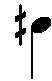
\includegraphics[height=15pt]{qt_c-cih}}}$	& a note raised by one \acl{qt}\\
	$\vcenter{\hbox{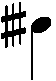
\includegraphics[height=15pt]{qt_c-cisih}}}$	& a note raised by three \aclp{qt}\\
\end{tabularx}

% list of acronyms
\newpage
\acbarrier % don't consider page numbers of abbreviations mentioned till here (to avoid non-content page numbers)
\vspace*{-2cm}
{\Huge \textbf{List of Acronyms}}\\[.3cm]
\addcontentsline{toc}{chapter}{List of Acronyms}
\begin{multicols}{2}
	\printacronyms
\end{multicols}

% set pages header and footers (moved from preamble because only need headers from here on (and better be after all lists etc.))
%-----------------------------
\clearpage % start new layout from next page
\pagestyle{fancy} % reset layout
\renewcommand{\headrulewidth}{0.4pt} % revive header line
\renewcommand{\chaptermark}[1]{\markboth{Chapter~\thechapter~--~#1}{}} % customize chapter header
\renewcommand{\sectionmark}[1]{\markright{\thesection\quad#1}} % customize subsection header
%\fancyhead{} % reset header
\fancyhead[LO]{\leftmark} % set right header on odd pages
\fancyhead[RE]{\rightmark} % set leftheader on odd pages

\addtocounter{page}{1} % reset page counter after preface
\pagenumbering{arabic} % switch to arabic page numbers

% Parts and Chapters
% ------------------

\part{Background}
\label{part:background}

\chapter{Introduction}
\label{chap:introduction}

\lettrine{I}{ntroduction} chapter -- motivation and goals plus outline

\pagebreak

\section{Motivation and goals}
\label{sec:motivation_and_goals}

People tend to adopt certain behavioral patterns from one another while interacting.
These may range from simple physical postures to language usage and even emotional reactions.
The overarching term for this phenomenon is \emph{accommodation} and it is commonly occurring in \acl{hhi}.
As explained by \acl{cat} from the 1970s, accommodation often has a social motive and it is used, even if unconsciously, to identify oneself with certain addressees or to trigger greater likability among a social group \citep{Giles2007CAT}.
It is theorized that the intrinsic motivation for this mechanism is a decrease (or an increase) of the social distance between interlocutors and the improvement of the interaction's overall efficiency \citep{Gallois2015CAT}.
Various empirical experiments have found accommodation effects in a variety of modalities, like facial expressions \citep{Kinsbourne2009embodied}, eye gaze \citep{Leong2017speaker}, lexical choices \citep{Brennan1996lexical}, and more.
Changes in speech, and especially low-level phonetic ones, are sometimes more subtle and harder to spot, e.g., than a mimic of body posture or the repeated use of a specific word.
Nevertheless, accommodation effects have been found in speech-related features, like speech rate \citep{Levitan2011measuring, Local2007phonetic} and pitch contour \citep{Babel2012role}.

The automatic utilization of accommodation strategies by speakers makes it an integral part of human communication.
However, in recent years, the everyday usage of voice-activated devices has been consistently increasing.
This kind of interaction introduces new challenges and coerces humans to adjust their verbal communication to cope with the limited capabilities of computer-based interlocutors.
While similar accommodation effects have also been found in \acl{hci} in different experimental settings \citep[e.g.,][]{Bell2003prosodic, Levitan2013entrainment, Parent2010lexical}, these were only remarkably limited on the non-human side.
\todo{change this sentence to be clear that the humans accommodated, but the computer side was very limited at best}
Such one-sided adaptation is incongruous with the mutual, dynamic exchanges occurring in \acl{hhi}.
Expanding the effect to computer interlocutors to simulate the aforementioned conversational dynamics still poses a challenge.
This challenge comprises both technical and modeling facets.
The former deals with the ability of a system to detect phonetic changes in the human's speech and to manipulate the corresponding features in its output speech in real-time, while the latter refers to determining the relationship between a user's realizations and the way they influence the system's productions.
Direct control over synthesized speech is challenging due to the limitations of current \acl{tts} synthesis methods, which almost exclusively use a trained model that cannot be modified on-the-fly.
\todo{probably need to improve this statement}
Even if such capabilities are achieved, accommodation models are required for establishing the way the system responds to users' speech variations.
This involves some design decisions.
For example, should the system try to simulate behaviors observed in \aclp{hhi} or simply follow the user's lead?
Should the system initiate changes or only react to user variation?
Could the course of the interaction be influenced by the way the system adapts towards the user?
All these decisions are part of defining the dynamics between the human and computer interlocutors and may change depending on the specific application.

Integration of accommodation capabilities can be especially beneficial for \aclp{sds}, as they are typically the core of verbal \acl{hci}.
Like improvements in other aspects of \aclp{sds}, vocal accommodation capabilities will contribute to their enhancement toward more human-like conversational behavior \citep{Weise2017towards}.
Considering the assumptions of \acl{cat}, interacting with a system that simulates behaviors familiar from \acl{hhi} should ease the process for the user and ultimately make it more efficient and fluent.
Furthermore, with the usage growth of voice-activated devices like \aclp{pa}, accommodative speech would offer additional degrees of personalization for users.
For instance, the speech of a \acl{pa} owned by one user might differ from that of another and could change when encountering a new user -- therefore reflecting the adjustments performed by humans.
Furthermore, studying accommodation in \acl{hci} shed light on the way humans perceive non-human interlocutors in social contexts and whether they want to communicate with them in a similar manner as with other humans.
\citet{Benus2018prosodic} show that a computer-based interlocutor gained more trust from human companions when it exhibited some level of vocal accommodation.

This work investigates the building blocks on the way to achieving vocal accommodation in \acl{hci}.
These include experiments for collecting evidence of accommodative behaviors in \acl{hhi} and \acl{hci}, approaches for modeling these behaviors in a computer-compatible fashion, methods for integrating accommodation models into real-time \acl{tts} synthesis, and implementation of a \acl{sds} that support vocal accommodation.
Previous work has addressed these concepts, mostly independently of each other.
\citet{Levitan2016implementing} introduce an approach for integrating prosodic-acoustic convergence into a conversational avatar, but without considering different types of accommodative behaviors.
Similarly, \citet{Bevnuvs2014social} examines social aspects of entrainment in spoken interactions, but does not demonstrate how those can be harnessed to measure them and develop models.
Obviously, the scope of each study cannot possibly cover all topics.
However, in addition to the depth of each of these concepts, the connections between them for introducing a complete solution should be considered as well.
For example, the manner in which the experimental findings are converted into a model defines the flexibility and degree of variation of the system.
It is therefore important to jointly address both the theoretical and technical facets of the topic, as they can benefit each other.
On the one hand, the technical capability to manipulate speech needs a modeled knowledge about the possible (and plausible) changes that might occur; and on the other hand, accumulating empirical data without showing how it models the phenomenon in question makes it highly challenging to demonstrate the essence of the captured evidence.

Offering such a comprehensive overview of this multidisciplinary theme and presenting the individual topics in a wider context were the primary inspirations for this work.
A further motivation was to suggest a more structural approach to accommodation description in computers, namely a hierarchy of accommodation levels.
Each level builds on the previous one and progressively increases the complexity and variability of the accommodative behavior, from direct mirroring of users' productions to independent responses
To that end, empirical data is required for observing a range of behaviors, and appropriate computational means need to be utilized to prevent too simple or unnecessarily complex behaviors.
This distinguishment between different types of behavior has received little to no attention so far and can help to better define the desired behavior of a system, based on user's expectation and the target application.
Lastly, an emphasis is put on the temporal aspect of conversation -- and by extension, of accommodation effects -- throughout the work, which is often neglected in studies, but provides important insights on the interactions' dynamics.

\section{Outline}
\label{outline} % intentionally doesn't have prefix sec: 

This work lies at the intersection of two communication phenomena, viz.\ \emph{phonetic accommodation} and \emph{\acl{hci}}.
Both of these topics play a role when talking with any kind of \emph{\acl{sds}}.
The challenges in combining them stem from the complexity and variability of accommodation processes and the absence of this inherent human capability in computers.
The core parts are structured to reflect the journey from theoretical ideas and empirical experiments, through modeling, and ultimately implementation of potential applications.

\Cref{part:background} introduces the main topics related to this intertwinement of research areas.
\Cref{chap:phonetic_convergence} provides an overview of the theoretical, social, and linguistic aspects of accommodation in general, and in spoken language in particular.
This includes types of mutual variation throughout a conversation and measurement of accommodation in \acl{hci}.
A survey of the ways humans interact with machines is presented in \cref{chap:spoken_dialogue_systems}.
The properties and challenges of verbal interaction with computers are discussed as well.
This chapter also introduces \aclp{sds}, along with their typical architecture and examples of common modern applications of them.
Finally, a suggested roadmap for integrating accommodation capabilities into \aclp{sds} is explained, together with terminology for differentiating some levels of accommodation in computers.

The main contributions are subsequently divided into three parts: Experiments, Modeling, and Application.
A series of empirical accommodation experiments are described in \cref{part:experiments}, each in a different social context and constellation of interlocutors.
\Cref{chap:conv_analysis} shows vocal accommodation effects and their utilization in real-world \emph{\acl{hhi}}.
Examining these effects in such conversations helps to determine the gaps between the analysis of conversations in the wild and lab setting.
Due to the length of these conversations, analyses of both dynamic changes over time and more general classification of speaker type are possible.
\Cref{chap:shadowing_in_sung_music_and_human_computer_interaction} presents shadowing tasks combining both \emph{\acl{hhi}} and \emph{\acl{hci}} contexts.
These tasks were carried out in closely controlled experimental settings for direct comparison between the two contexts.
Further evidence of accommodation in a different context is explored in a study of vocal accommodation in \emph{singing}.
Lastly, a multiparty \emph{\acl{hhci}} study is outlined in \cref{chap:speech_variations_in_hhci}.
This more evolved mix of speakers sheds light on accommodation effects influenced by the addressee of the specific utterance or by the presence of another human interlocutor.

\Cref{part:modeling} comprises two approaches for modeling accommodation to be used in a \acl{sds}.
A computational model composed of empirically-motivated parameters is introduced in \cref{chap:computational_model}.
This model aims to provide a descriptive way to depict accommodation and craft desired behaviors.
The approach taken in \cref{chap:statistical_model} is statistical in nature.
It identifies different speaker tendencies, even if those cannot be explicitly be broken into specific properties.
Nevertheless, these can be used for defining a target behavior for a system.
The use of these two approaches in conjunction is also discussed.

\Cref{part:application} contains implementations of components required for responsive \aclp{sds}.
The technical details of a module linking between the speech input and output of a system are described in \cref{chap:convergence_module_for_sdss}.
This includes an additional module for handling accommodation-related processes, like detecting variable sounds and running the model, and a brief survey of real-time, on-demand manipulation of synthesized speech, which enables the required control over a system's output needed for realizing accommodation effects.
Together with the modeling information and the techniques from \cref{part:modeling}, these components are utilized in the system introduced in \cref{chap:web-based_responsive_spoken_dialogue_system}.
The extended architecture, usage possibilities, and graphical visualizations of this system are demonstrated via a use-case display.

\label{outline_end}

\pagebreak

\section{Related own publications}
\label{sec:related_own_publications}

\begin{longtable}{m{.35\linewidth}m{.6\linewidth}}
	\toprule
	{\large \bfseries \Cref{chap:shadowing_in_sung_music_and_human_computer_interaction} --\newline\newline \nameref{chap:shadowing_in_sung_music_and_human_computer_interaction}} &
	\fullcite{Raveh2020SpeechProsody}\newline\newline
	\fullcite{Raveh2017ESSV}\\
	%
	\midrule
	%
	{\large \bfseries \Cref{chap:speech_variations_in_hhci} --\newline\newline \nameref{chap:speech_variations_in_hhci}} &
	\fullcite{Raveh2019InterspeechAlexa}\newline\newline
	\fullcite{Raveh2019ESSV}\\
	%
	\midrule
	%
	{\large \bfseries \Cref{chap:computational_model} --\newline\newline \nameref{chap:computational_model}} &
	\fullcite{Raveh2017Interspeech}\newline\newline
	\fullcite{Raveh2019PundP}\\
	%
	\midrule
	%
	{\large \bfseries \Cref{chap:convergence_module_for_sdss} --\newline\newline \nameref{chap:convergence_module_for_sdss}} &
	\fullcite{Raveh2017SemDial}\newline\newline
	\fullcite{Raveh2017PundP}\\
	%
	\midrule
	%
	{\large \bfseries \Cref{chap:web-based_responsive_spoken_dialogue_system} --\newline\newline \nameref{chap:web-based_responsive_spoken_dialogue_system}} &
	\fullcite{Raveh2018Specom}\newline\newline
	\fullcite{Raveh2021ICASSP}\\
	\bottomrule	
\end{longtable}
\chapter{Phonetic Accommodation}
\label{chap:phonetic_convergence}

\lettrine{I}{n} this chapter, the concept of accommodation is introduced.
Types of linguistic changes and they way similar terms are used in this work are explained as well.
Finally, a survey of works on phonetic convergence in \acl{hci} lays the ground to the novel work presented in this work.

\pagebreak

\section{\Acl{cat}}
\label{sec:communication_accommodation_theory}

Communication is a fundamental part of life.
In addition to offering a means to exchange information and express emotions and desires, it also exhibits salient social category memberships
Human communication is a complex concept concealing many facets and sub-processes within it.
This Complexity stems from two main aspects:
First, each individual is unique and communicates differently -- in general as well as in specific interactions -- based on inherent traits, emotional state, personal preferences, situational circumstances, and more.
Moreover, an interlocutor may belong to a certain group or represent one (e.g., a social group or an organization), which may also influence the nature of the exchange.
Secondly, some forms of communication, in particular face-to-face, harness combinations of modalities.
This results in a large amount of data one needs to process in real-time to obtain maximal efficiency.
Furthermore, despite common social conventions, not every person perceives and processes this information the same way, which requires all interlocutors to be attentive as they how they comprehend the others and are being understood by them.
Therefore, each exchange is unique and shaped by various personal and environmental factors (more in  \cref{subsec:dialogue_is_hard}).
To cope with such highly variable dynamics, people must have some way to know -- whether unconsciously, intuitively, or deliberately -- how to adjust their communicative behavior.

\Acf{cat} is a theoretical framework of communication introduced by \citet{Giles1973mobility, Giles1991CAT, Giles2007CAT}, which aims to explain the personal and social motivations in verbal and non-verbal human communication.
A core motivation in \ac{cat} is \emph{social distance}.
To reduce social distance, a speaker may converge to the conversation partner(s), whereas divergence would lead to an increase in social distance.
When and how social distance should be altered depends on the social class of the speakers, their formal role and personal goals in the interaction, etc.
Particularly, these changes occur with respect to how the other conversation partners speak, from overall psychological, social, and linguistic behaviors to specific features (like those in \cref{sec:linguistic_accommodation}).
For example, different communication styles would probably be utilized when speaking to a childhood friend, a colleague, or a company's executive.
In each of these situations, the speakers would likely use different language registers (e.g., slang words and politeness) in an attempt to fit into the social groups or become socially closer.
Another example is the use of \enquote{elder language} when talking to old people (e.g., talking more slowly, extended use of hand gestures, etc.), to make it easier for them to understand the speaker.
Such adjustments can be, to some extent, conscious, but often occur automatically.
Ideally, both speakers find their comfort zone during the conversation.
However, there exist the notion of over-accommodation, which is usually a result of a very conscious speaker that intentionally exploits this phenomenon.
If realized by a conversation partner, this might be perceived as pretentious or fake behavior and even mockery.
Similarly, accommodation can serve a speaker with audience design when talking to a larger group of people.
The adjustments may be reflected simultaneously in different modalities, like hand gestures, body posture, facial expression, eye gaze, lexical choices, and speech.
This work concentrates on linguistic aspects and speech in particular.
Detailed examples of linguistic accommodation are described in \cref{sec:linguistic_accommodation}.
While \ac{cat} advocates these changes, it is worth mentioning that there are other further frameworks that explain them as well.
For instance, the Interactive Alignment Model \citep{Pickering2004behavioral, Pickering2013integrated} offers a model where adjustments in communicative behavior are described as \emph{alignment} as opposed to \emph{accommodation}, hinting that the process is rather one-sided and uni-directional (see \cref{tab:variation_types}).
Despite this difference and others, all these frameworks describe a process where the similarity between interlocutors increases or decreases with respect to certain features over the course of their communication.
\Cref{subsec:variation_types} sheds more light on the difference between the different terms used to describe this process and how they are used in the literature.

\subsection{Variation types -- terminology}
\label{subsec:variation_types}

The term \enquote{convergence} is a central notion in this work.
This term's definition in this work is different from its meaning in other fields, like \ac{ml}.
Moreover, numerous terms are used in the literature synonymously to describe the same phenomena, although there are often subtle differences or emphases on specific angles of it.
Disambiguate these various terms should help to avoid confusion and allow a more fine-grained description of such processes.
The core meaning of convergence is explained here in detail, followed by a list of related terms and explanations about their use in the literature.

The verb \textit{to converge} is defined in Cambridge Dictionary\footnote{\url{http://dictionary.cambridge.org/dictionary/english/converge}} as moving toward, or merging into, the same point (e.g., roads).
A more non-materialistic definition is provided as well: \enquote{If ideas and opinions converge, they gradually become similar}.
Another, somewhat more general, definition to the noun \textit{convergence} is given in Merriam-Webster dictionary\footnote{\url{https://www.merriam-webster.com/dictionary/convergence}}: \enquote{the act of converging and especially moving toward union or uniformity}.
As all these definitions suggest, the core idea of this concept is two (or more) entities that change (potentially in different degrees) toward some physical or abstract point and ultimately meet.
In some time-dependent cases, like spoken interactions, this point can be expected to be within the range of the entities (the speakers).
Furthermore, in such cases, there might not be enough time for them to meet, but to become closer, more similar, to one another nonetheless.
This matches the definition of \emph{phonetic convergence} proposed by \citet{Pardo2006phonetic}: \enquote{[\ldots] increase in segmental and suprasegmental similarities between two speakers}.
This also resembles the definition suggested by \citet{Xia2014prosodic}: \enquote{[\ldots] behaviors become more similar over time}, with \enquote{behaviors} referring to different modalities of communications in conversation, e.g., facial expressions, gestures, lexical choices, etc.
Other terms are sometimes used to describe similar processes or different aspects, and it is important to make the distinction between them.
Note that some of the terms are used interchangeably, as synonyms, or as hypernyms and hyponyms in other works.

The list presented here aims to unequivocally distinguish these terms and grant them useful relations to offer a meaningful common terminology, at the very least within the scope of this work and hopefully in the community of this research area in general.
\cref{tab:variation_types} summarizes the comparison of the terms' characteristics.

\begin{table}[t]
	\centering
	\caption[Comparison of variation types]
		{Comparison of variation types properties.
		[explain each column]
		A \partick  sign indicates that the property is fulfilled to some extent, or that it may be potentially implied or assumed in some cases.
		The \enquote*{*} signs mark the terms most widely used in the literature.}
	\label{tab:variation_types}
	\begin{tabularx}{\linewidth}{Xcccc}
		\toprule
								& mutuality & directionality & intention/awareness & defined target\\
		\midrule
		accommodation*			&	\partick	&				&				&				\\
		\rowcolor{lightgray}
		convergence*			&	\partick	&	\tick		&	\partick	&				\\
		mimicry					&	\partick	&	\tick		&	\partick	&	\partick	\\
		\rowcolor{lightgray}
		proximity				&	\tick		&				&				&				\\		
		synchrony				&	\tick		&	\partick	&				&				\\
		\rowcolor{lightgray}
		mirroring				&	\tick		&	\tick		&				&	\tick		\\
		coordination			&	\tick		&	\partick	&	\tick		&	\partick	\\
		\rowcolor{lightgray}
		assimilation			&				&	\tick		&	\partick	&	\partick	\\
		adaptation*				&				&	\partick	&	\tick		&	\tick		\\
		\rowcolor{lightgray}
		chameleon eff.			&				&	\tick		&				&	\partick	\\
		priming					&				&	\tick		&				&	\tick		\\
		\rowcolor{lightgray}
		entrainment*			&				&	\tick		&	\partick	&	\partick	\\
		alignment				&				&	\tick		&	\partick	&	\tick		\\
		\rowcolor{lightgray}
		imitation				&				&	\tick		&	\tick		&	\tick		\\
%		int.sp. influence		&						&	\tick		&	\partick				&	\partick			\\
		\bottomrule
	\end{tabularx}
	\todo[inline]{any other properties to have in table for more fine-grained distinction?}
\end{table}

\begin{description}
	\item[accommodation] -- is often used in the literature as an overarching term derived from its meaning in \ac{cat} and includes any dynamic mutual changes during an interaction.
	Specifically, it includes both convergence and divergence, but also other forms of change caused by influences of other interlocutors.
	An important aspect of any accommodative effect is that it is a result of external input.
	Therefore, \acp{sds} with accommodative capabilities are described as \emph{responsive} in \cref{subsec:accommodation_levels} (and see example in~\cref{fig:validation_sensitivity}).
	
	\item[convergence] -- As explained above, convergence means an increase in similarity between the speakers (see illustration in Figure 1 in \citet{Levitan2011measuring}).
	Each speaker can account for a different \enquote{amount} of the convergence, based on the speaker's tendency to converge in the specific interaction and in general.
	There may be great individual differences in this tendency, as shown in the experiments in \cref{part:experiments}.
	This tendency is referred to as the speaker's \emph{sensitivity} to external changes in \cref{sec:parameters}.
	Convergence can result in the speakers' production values \enquote{meet} somewhere in the middle (as in \cref{fig:accommodation_types}) or closer to one of them, depending on the social dynamics in the interaction.
	
	Similarly, \textbf{divergence} is the reversed effect, i.e., when a decrease in the similarity between the speakers occurs.
	Divergence is generally less common in \ac{hhi}, but may occur in competitive, as opposed to collaborative, scenarios, or when a speaker, intentionally or not, thrives to deliberately be distinguished from the other.
	
	\item[entrainment] -- is presented by \citet{Brennan1996lexical} as the (potentially aware) influence of an interlocutor on another, e.g., imposing lexical units in an interaction, with emphasis on the one-sided nature of the process.
	This means that one of the interlocutors established the use of an aforementioned term which created a bias by the conversation partner to employ it as well.
	The change is sometimes seen as categorical (similar to \textit{priming}), which is a key difference from the definition of convergence here.
	This is especially relevant in \ac{hci}, as it is much easier for a computer, due to the vocabulary problem \citep{Furnas1987vocabulary}, to establish such uses.
	\citet{Lopes2013automated} describe entrainment as imposed by a human speaker, where a computer-based interlocutor follows the lexical choices of the user.
	This term is sometimes also used as a static measure of changes in an interaction (cf.\ \cref{subsec:limitations_of_did}), as in \citet{Levitan2013entrainment}.
	Conversely, \emph{convergence} refers here to the potentially mutual dynamic measure, the difference being comparing discrete timestamps in the interaction (for example, between two halves of a session, as done by \citet{Xia2014prosodic}) versus changes occurring gradually over its entire length.
	In addition to all the above, entrainment is often synonymous with convergence or accommodation in more technical fields.
	
	\item[synchrony] -- refers to an ongoing process where the interlocutors are changing their behavior similarly, i.e., synchronously.
	Importantly, this applies to the relative change in each speaker, but not to any absolute values.
	That is, the distance is generally maintained while the individual ranges may differ (see Figure 1 in \citet{Levitan2011measuring}).
	When one of the speakers is leading the synchrony, it becomes \emph{lagged}, as shown in \cref{fig:accommodation_types}.
	Lagged phenomena are often identified, and their leader determined, using some correlation measure, like Peasrson's coefficient in \citet{Edlund2009pause, Xia2014prosodic}.
	A deeper analysis of such an accommodation effect is presented in \cref{sec:analysis_hhi}.
	
	\item[adaptation] -- refers to the process of making intentional changes that suit certain conditions or situations.
	As such, this term stresses the ambition of these aware modifications in vocal behavior made by an interlocutor to be more similar to another, known and defined, target exhibited by another speaker.
	\citet{Kang2010emergence, Hwang2015phonetic} both examine the phonetic adaptation process that occurs gradually when encountering a new sound environment, to which speakers want or are expected to adapt.
	In these cases, the changes are also likely to be maintained outside the scope of a specific interaction.
	Adaptation is also used to describe the technical capability -- or more often the lack of one -- in a machine to match its speech production (typically to a user talking with the system).
	This fits the definition of adaptation being intentional and having a well-defined target to adapt towards.
	However, this is still a very limited feature due to the state of \ac{tts} technologies.
	The challenges and integration of such capabilities into \acp{sds} are discussed in \cref{sec:adaptive_spoken_dialogue_systems,chap:convergence_module_for_sdss}.
	
	\item[priming] -- is similar to entrainment, but usually works on a larger scope -- in terms of both time and degree of change.
	It is typically used in the context of psycholinguistics.
	As opposed to entrainment, e.g., on the lexical level, priming can influence not just the use of one specific term, but a whole semantic field.
	For example, it was shown in experiments by \citet{Meyer1971facilitation, Schvaneveldt1973retrieval} that people respond faster to words from a specific semantic field after being exposed to other words from it over a long timespan.
	% (i.e., different words that are semantically related).
	In more general terms, priming changes the likelihood of a person to use specific behavior, typically on some semantic or syntactic level.
	The temporal scope is different as well.
	Priming can have an effect in a longer-term than a single interaction, ranging from multiple interactions across several hours, days, and up to years.
	Therefore, this term is often used when talking about language change in children \citep[see, e.g., ][]{Huttenlocher2004syntactic, Wansink2012would}.
	Like entrainment, priming also typically describe a categorical change, as opposed to gradual change on a scale (see \textit{entrainment} and cf.\ \citet{Reitter2006computational, Pace2013concept}).
	
	\item[assimilation] -- implies a one-sided process, where one side changes in a certain way to match the other.
	It is typically used to describe an accommodative process with the motivation to associate oneself with a social group by adopting its vocal characteristics.
	Therefore, assimilation is seen as a change that occurs as a result of a specific situation or context, e.g., public speeches, as shown by \citet{Ohala1990phonetics} in \cref{subsec:sound_change}.
	Similarly, in phonology, this term is used to describe a sound that changes to become similar to another sound with respect to a certain feature \citep[see examples in][pp.~89-98]{Hall2011phonologie}.
	%	e.g., when voiceness of a sound changes to match this of the sound adjacent to it.
	%	Note that assimilation is only one of the phonological processes (others would be dissimilation, epenthesis, elision, and more), but since it's the once describing two things becoming more similar to each other, it is the one that might be used in this context.
	
	\item[alignment] -- is a term used in the Interactive Alignment Model \citep{Pickering2004behavioral}, which describes an increase in similarity between speakers.
	It describes a process similar to assimilation, but with certain motivations and behind it.
	While in assimilation the change is measured with respect to a social group or speech style, alignment refers to general changes without such a specific target.
	Specifically, it is claimed to contribute to the overall ease and success of conversations by the interlocutors to behave similarly on different linguistic levels \citep{Garrod2009joint}.  
	
	\item[mirroring] -- the potentially unaware cognitive effort to produce an output that follows some input.
	A.k.a.\ \enquote{mirrored equivalence} \citep{Messum2015creating, Messum2007mirroring}, this process differs from imitation by the lack of aim toward a well-defined target, but rather an internal representation of the similarity between the speakers.
	This may lead to a less planned and sometimes automatic effect of becoming closer to an interlocutor, where the specifications of the change do not necessarily match the input target.
	Less commonly, this term also refers to an effect opposite to synchrony, where the directions of the respective changes are reversed instead of similar (as if a mirror was put between them).
	Additionally, mirroring may also refer to an effect similar to mimicry, but with greater emphasis on speech learning and acquisition \citep[e.g.,][]{Yoshikawa2003constructivist}.
	
	\item[mimicry] -- is the tendency to behave, or speak, broadly like someone else.
	The emphasis here is on the \emph{general} inclination, which hints it can be done unintentionally, or, alternatively, be deliberate, but without the goal to perfectly match the target (as opposed to imitation).
	% inspired by https://www.voices.com/blog/mimicry_vs_imitation/
	\citet{Gueguen2009mimicry} demonstrate how mimicry can earn the mimicker more favorable judgment in social interactions.
	This is explained by mimicking creating a greater feeling of affiliation and rapport in communication, or with the more positive evaluation of the mimicked person due to an enhanced familiarity established by the mimicker.
	\citet{Parrill2006seeing} show just how natural mimicry is in \ac{hhi} in an experiment where participants' behavior was affected merely by watching mimicking takes place in another conversation.
%	reference, mention \textit{Chameleon effect}\ldots
	
	\item[imitation] -- similar to mimicry, but is done intentionally and with the goal to match as closely as possible to a target.
	In addition, emphasizes the speaker's intent to completely match the auditory input \citep[cf.][]{Gueguen2009mimicry}.
	% inspired by https://www.voices.com/blog/mimicry_vs_imitation/
	The attempt to \emph{deliberately} repeat and \emph{accurately} replicate another speaker's productions distinguishes imitation from mirroring and mimicry.
	
	\item[chameleon effect] -- is a more general account of mimicry, but with complete non-conscious adoption of an interlocutor's behavior \citep{Chartrand1999chameleon}.
	It is a social psychology term typically associated with a comprehensive change in multiple modalities and in the overall mannerisms.
	\citet{Gueguen2009mimicry} focus on the social aspects of this effect and how it can change social judgment and attitude toward the speaker.
	Both authors describe it as "monkey see, monkey do", which emphasizes the automatic nature of it.
	Moreover, they state that it is a learning mechanism for children and for humans in general before the development of unified languages \citet[][p.\ 256]{Gueguen2009mimicry}.
	
	\item[proximity] -- describes general closeness between interlocutors (as illustrated in Figure 1 in \citet{Levitan2011measuring}).
	This does not imply specific distance thresholds or absolute value ranges.
	Furthermore, this is a rather passive, potentially merely circumstantial, situation, which does not involve a vocal target or an aspiration to match it.
	The proximity at a specific point in time (typically around the start of a conversation) can be used as a reference point for other measures.
	
	\item[coordination] -- implies cooperation -- either seeming or real -- between the interlocutors, i.e., that there is a common goal to achieve.
	Increase or decrease of communication features is in this case a side of effect of this coordination.
	This provides another point of view on the process, namely not to examine the speakers' collaboration based on common changes, but looking at the changes knowing they are collaborating.
	
%	\item[inter-speaker influence] -- a general term to describe a change by a human interlocutor caused by another.
\end{description}

\section{Linguistic accommodation}
\label{sec:linguistic_accommodation}

Accommodation occurs on various linguistic levels in \ac{hhi}.
Relative salient changes may occur on the lexical level when one interlocutor shifts his lexical choices to match those of another.
This is more likely to happen when a lexical entity has multiple commonly used alternatives, like synonyms or different names.
\citet{Jucks2008lexical} show how healthcare experts try to match their wording to patients in written inquiries.
In another experiment, \citet{Friedberg2012lexical} found increasing lexical similarity over the course of spoken discussion among students groups with better performances.
\citet{Racz2020morphological} even extended the analysis to morphological forms, suggesting that morphological convergence occurs and creates generalizations in memory in real-time.
over these instances.
Other examples of lexical convergence have also been found in \ac{hci} when looking for information \citep{Lopes2013lexical} and when playing \citep{Bergqvist2020nontrivial} (and see \cref{subsec:previous_work}).
In all these experiments, it was shown that lexical convergence had a positive effect on the performance of the speakers.

The focus in this work is on accommodation occurring in speech-related features, i.e., \emph{vocal accommodation}.
A core difference between lexical and vocal accommodation is the mechanism for defining two instances as the same.
For example, the word \enquote{window} is written the same way regardless of who writes it (this is especially true if the word typed), which makes it easy to associate tokens with the same type.
However, vocal features are strongly dependent on the speaker.
The signal representing a word would be different depending on the speaker's physiological properties (like vocal tract size), natural speaking rate, voice intensity, intonations, and many more.
Moreover, it is very unlikely that even the same speaker would pronounce the same word in the same manner.
This is especially true in conversation taking place in different settings and environments, but also for two successive utterances in the same conversation.
Additionally, the relative differences, e.g., in vowel quality or speaking rate, also differ from one person to another, which entails that more evidence might be needed for a perceivable target for accommodation to emerge.
An exception to these differences could be categorical phonetic differences, where each category may be perceived as a separate entity (similarly to the lexical case), making it easier to define the target (and see \cref{subsec:target_features_HCIConv,subsec:speech_manipulation}).
This great variety in spoken language makes the accommodation process somewhat more complex, as the targets might not always be well-defined and static.
%(comparing with a lexical entity that would always be recognized as the same).

Vocal accommodation has been found in both segmental \citep{Pardo2010conversational, Smith2007prosodic} and suprasegmental \citep{Walker2015repeat, Shockley2004imitation} phonetic features and
both in conversational \citep{Pardo2006phonetic, Lewandowski2012talent, Weise2018looking} and non-conversational \citep{Babel2014novelty, Shockley2004imitation} scenarios.
There is evidence for it being both an internal mechanism \citep{Pickering2004behavioral} and socially motivated \citep{Kim2011phonetic, Giles1991CAT, Babel2010dialect}.
For instance, phonetic convergence \citep{Giles1973mobility} or divergence \citep{Bourhis1977distinctiveness} is triggered by decreasing or increasing social distance between interlocutors, respectively.
\Citet{Baumann2020how} even shows that feedback given by conversation partners can influence the convergence process.
As demonstrated by \citet{Pardo2013measuring}, vocal accommodation can occur with respect to numerous phonetic features.
\citet{Aubanel2020speaking} found that speakers accurately and consistently converge to each other's pitch (\ac{f0}) in scripted read-aloud dyadic conversation on a turn-by-turn basis.
This shows the ability to track changing \ac{f0} both in perception and production.
The study conducted in \citet{Babel2012role} supports the importance of \ac{f0} in convergence effects by showing that filtering out the \ac{f0} frequencies in the signals the participants hear leads to reduced convergence.
\citet{Schweitzer2017visibility} show that convergence effects are stronger when conversation partners can speak but not see each other, and divergence occurs more when they can also see each other while talking.
Moreover, the effects were stronger depending on the degree of likability between them.
This shows that accommodation can be influenced by other, not necessarily linguistic factors of the conversation.
According to \citet{Lehnert2020relationship}, language skill level and greater \ac{f0} expressiveness also influence the degree of convergence.
Accommodation effects were also found in intensity.
In an experiment where participants heard an interviewer in different levels of vocal intensity, \citet{Natale1975convergence} shows that their intensity was generally changed accordingly.
In a second experiment, the degree of intensity convergence could be predicted by a social desirability test, which stands in line with the finding of \ac{f0} accommodation.
A third studied feature is speaking rate (and sometimes \acf{ar}).
In an exemplar-theoretic view in mind, \citet{Schweitzer2016exemplar} investigated how syllable frequency influences the degree of change.
Evidently, stronger effects were found in more frequent syllables, which supports this view.
Relatedly, \citet{Edlund2009pause, Xiao2015analyzing, Cohen2017converging} introduce ways to measure temporal prosodic changes, like pauses, in conversation, which affect the speaking rate.
\citet{Levitan2011measuring, Local2007phonetic} found convergence effects in all these three features (and others) in collaborative games and every-day scenarios.
Such a wide variety of evidence suggests that, even in the vocal modality alone, accommodation is reflected in various ways in \acp{hhi}.
These features are investigated in this work in both \ac{hhi} (\cref{chap:conv_analysis}) and \ac{hci} (\cref{chap:speech_variations_in_hhci}) contexts.
In addition to these, other factors and phonetic features were investigated for accommodation, such as voice quality \citep{Borrie2017conversational}, voice onset time \citep{Nielsen2011specificity}, and other timing-related phenomena \citep{Putman1984conception}, second language proficiency \citep{Law2020convergence}, interlocutors' sex \citep{Levitan2012acoustic, Bailly2014assessing}, perceived attractiveness \citep{Michalsky2017pitch}, word frequency \citep{Nenkova2008high}, and more.
Further methods and ways to measure accommodation in \ac{hhi} can be found in \citet{Lewandowski2019phonetic, DeLooze2014investigating}.

\subsection{Long-term and short-term sound changes}
\label{subsec:sound_change}

All the sound changes discussed in this work are short-term changes occurring over the timespan of a single, even if long, interaction (e.g., \cref{chap:conv_analysis}) or a series of following interactions (e.g., \cref{chap:speech_variations_in_hhci}).
Similarly, the models and applications in \crefrange{chap:computational_model}{chap:web-based_responsive_spoken_dialogue_system} are also designed to handle accommodation-related changes within the scope of time-limited interactions.
However, sound change may occur continuously over long periods of time -- even years or decades.
While short-term accommodative changes can be ascribed to local social influences of specific interlocutors (see \cref{sec:communication_accommodation_theory}), long-term changes may stem from larger cultural influences and independent evolution of the person's speech.
In both cases, the change's source can be both the speaker and the listener \citep[][pp.~176-187]{Ohala1989sound} and is typically caused by confusion or correction \citep{Ohala1993phonetics}.
The latter is more relevant, for instance, for short-term assimilation, as demonstrated in \citet{Ohala1990phonetics}.
The former, however, is more dominant in long-term changes and cross-language influences, e.g., when sounds in one language are replaced by similar sounds in another when loaning words.
This is also related to mutual influences of speakers in the evolution of a language, or the way different speaking styles can be created within a language to mark cultural, regional, and social differences.
These reasons and others are explained from the phonetic point of view in \citet{Sweet1874history}.

Such long-term changes can also occur in the speech of a single person.
\citet{Harrington2007evidence} examined vowel changes in the Queen's pronunciation in her annual Christmas messages from 1952 to 2002.
Some gradual changes were, indeed, found, but could not be ascribed to age or varying speech style.
The author, therefore, considered it an independent, long-term sound change of an individual.
Contrarily, in the pronunciations around the 1980s assimilation was found towards accents associated with younger people of lower classes \citep{Harrington2000does, Harrington2000monophthongal}.
This suggests a, potentially aware, audience design from the Queen's side \citep{Bell1984language}.
Such use of communication falls under the social motivation of \ac{cat}, although the interactions were one-sided.
In this example, the changes were not a result of interactions over a long period of time.
However, this may happen as well between people who speak often to each other for many years.
This is relevant for \acp{hci} that are designed to last a very long time, like \acp{pa} or social companion (see \cref{sec:types_of_sdss}).
Therefore, in such systems, accommodation effects should be taken into account as well, but the modeling approach could take advantage of the fact that there is a much longer timespan for the changes to unfold.
This can be used, for example, for accumulating more evidence before deciding on the appropriate change from the system side (cf.\ exemplar approach in \cref{chap:computational_model} and floor-change approach in \cref{chap:statistical_model}).

\subsection{Measuring accommodation} % Limitations of \acl{did} measures
\label{subsec:limitations_of_did}

Conversations are complex processes that require some expertise and some quantitative analysis to detect and isolate specific patterns in them.
All the more so, since effects may have long, non-linear relations.
A behavior is a complex collection of conducts of a person (and any organism, system, or artificial entity), particularly those towards a certain environment.
The realization of one's behavior over the course of a conversation can communicate information regarding one's state and goals, especially with this deviates from the individual's expected behavior.
The behavior leads to reactions to environmental input and can be modified due to reinforcements from the environment or self-directed motives.
These modifications can occur over time quickly or slowly, consciously or unconsciously, and to a greater or lesser extends, which makes them dynamic and thus cannot be defined discretely.
All the above is true also for vocal behaviors, which are expressed in spoken interactions.
Specifically, vocal accommodation reflects dynamic changes during a conversation that can be affected by the external speech input of other interlocutors.
It can therefore be beneficial to \textbf{move away from value comparisons in favor of behavior descriptors} to depict an interaction.
This is done by analyzing spoken interactions as entire events with a continuous temporal dimension as opposed to a comparison between some discrete points in time.
Examining the whole conversation can help, for example, to determine who was leading the changes or when more accommodation occurred.
In this work, such analyses were utilized in \cref{chap:conv_analysis} to determine the leading speaker in each conversation and in \cref{chap:speech_variations_in_hhci} to expose the ongoing changes in the human speaker's productions.

The way speakers accommodate to each other is very unlikely to be linear from beginning to end and can change throughout the conversation.
Therefore, comparing the differences between two discrete, distant points in time might miss or oversimplify some dynamics that occurred between them.
Moreover, comparisons like that must inherently take the view of one speaker instead of looking at the conversation as a complete entity.
Quantitative analyses often leave accommodation hidden or overly-simplified if analyzing a conversation on a turn-by-turn basis or by splitting it arbitrarily into two or more parts (often equally-long, non-overlapping time intervals) and directly comparing them using raw values as in \citet{Heldner2010pitch, Rahimi2018weighting, Ibrahim2019fundamental}.
\citet[][p.~15]{DeLooze2014investigating} points out that in these cases it is assumed that accommodation is a strictly local phenomenon where a speaker's utterance is linked exclusively to the other interlocutor's immediate preceding utterance.
Such analyses result in a linear, static representation of the conversation's evolution, from which generalized conclusions are hard to draw.
They might even be inaccurate or misleading, especially when both speakers change their output over time, as demonstrated by \citet{CohenPriva2019limitations}.
That work refers specifically to \ac{did} measurements, where pairs of two discrete points in time are compared to measure accommodation between speakers using the following distance formula\footnote{Note that this way of measuring \ac{did} is commutative and therefore doesn't measure the changes from the view of a specific speaker \citep[unlike,~e.g.,][p.~3]{CohenPriva2019limitations}.}
%
\begin{equation}
	\label{eq:did}
	DiD_{\vec{i},\vec{s}} \coloneqq \sqrt{(\vec{i}_{t + 1}^n - \vec{s}_{t + 1}^n)^2 + (\vec{i}_t^n - \vec{s}_t^n)^2} \equiv \lVert \vec{i} - \vec{s} \rVert_n.
\end{equation}
\eqname{\Acl{did} measure (simplified)}
\noindent
%
\cref{fig:accommodation_types} shows the interaction between two speakers' productions in a hypothetical conversation.
By merely looking at the plot, it is clear that the two speakers do not sustain the same behavior throughout the conversation.
For example, between marks A and B the orange speaker's values go remarkably downwards (though not linearly), while the green speaker remains roughly stable -- i.e., \emph{divergence} (although this can also be seen as an independent change).
Subsequently, the distance is generally maintained between B and C.
Between C and D \emph{convergence} occurs \textbf{in both speakers}.
Lastly, lagged \emph{synchrony} can be observed between marks D and E.
If compared directly, the lagging might make the value changes look somewhat random.
However, looking at the entire segment, it's clear that the change is similar and is led by the green speaker.
None of these mutual behaviors can be captured by a \ac{did}-based approach.
For instance, comparing the beginning (mark A) and end (mark E) of the conversation would lead to the conclusion that there was no change in the values (illustrated by the corresponding dashed lines).
Similarly, splitting the conversation into two halves (A to D and D to E) would make it look like the changes were symmetrical, missing the obviously different behaviors of the speakers in these two halves.
Additionally, the directionality of the convergence between marks C and D will be missed by simple \ac{did} distance measures, which might give the impression that the changed rooted from only one of the speakers.
This could be satisfactory when it can be assumed that such changes can only occur in one speaker, like when talking with some computer-based interlocutor like a \ac{pa} (\cref{sec:convergence_to_natural_and_synthetic_stimuli,sec:vacc}, but not when both speakers' productions may be flexible, like in \ac{hhi} (\cref{sec:analysis_hhi}) or ultimately adaptive \acl{sds} (\cref{sec:adaptive_spoken_dialogue_systems}).
This limitation can be compensated to some extent by examining the \emph{relative} occurring changes \emph{gradually} (\cref{fig:condition_convergence_comparison,subsec:temporal_analysis}).

%Methods used in time series analysis are utilized in this paper to detect and model long-term relations within a conversation.
%This approach offers different types of analyses and emphasizes the temporal aspect of spoken interactions.
%The first is \ac{crqa}, which is proportionate to the conversation's length.
%It measures the \emph{mutual} similarity changes of the speakers throughout the entire conversation in term of recurrence.
%Additionally, it tells when the recurrence segments sustained for longer periods and which speaker led them.
%\cref{sec:capturing_patterns_in_time_series} explains how this method is used to differentiate the dataset introduced in \cref{sec:dataset_and_feature_extraction} to define different profiles.
%Another method is neural autoencoder (\cref{subsec:dim_reduction}), which can learn non-linear representations in a latent space.
%This technique is good for creating generalized models based on many conversations and speakers.
%By using \ac{vae}, these models become generative and can therefore be used for producing varying speech output of a system fitting to its chosen profile or combination of profiles.
%Finally, \acp{gp} add stochastic Gaussian variability to the yielded output based on the function distribution derived from the models.
%Variations of the base behavior are produced that way.
%This is demonstrated in \cref{subsec:generation_gp_kriging}.

%As discussed in \cref{subsec:conversation-level_accommodation_behavior}, \ac{did} and sequential methods for measuring vocal changes (e.g., accommodation) rely on the chronological, turn-by-turn order of the interaction and their scope is limited to detect local phenomena only.
%Non-linear methods, contrarily, are not dependent on the chronological order of the interaction's turn and can therefore find long-term, more distant relations between the speakers with respect to the target feature.
%For instance, that an accommodation process (or generally closer values) occurred at some point in the beginning and continued at a later time, or that there was a periodic pattern of convergence and divergence throughout the interaction.
%Such phenomena point to more general, conversation-level properties that do not rely on the unfolding chronological order of the turns.
%This is especially useful for long interaction, where various patterns occur a more general view may be insightful (see example in \cref{fig:accommodation_types}).
%
%We take here a different view on the structure of the conversation, namely referring to it as a set of \emph{time series}.
%Time series is a sequence of chronologically ordered values sampled from some data stream along equal time intervals.
%Due to the way the dataset presented in \cref{sec:dataset_and_feature_extraction} is analyzed, the extracted features can be treated as couples of \emph{time series}, one for each speaker in each conversation.
%\todo{examples of where speech is treated as TS (ASR?)}
%Because of the nature of these features (and perhaps any spontaneous, interactive linguistic feature), the resulted time series can be assumed to be non-seasonal and non-stationary.
%\todo{might want to remove this sentence to not commit to this type of data}
%This view on the data enables a new assortment of analysis methods, from which \acf{crqa} and \acf{gp} are demonstrated here (\cref{subsec:crqa,subsec:generation_gp_kriging}).
%
%This recognition as time series opens new methodological possibilities for examining the evolution of these features and their realizations by different speakers in an interaction over time.
%Such methods include, among others, autocorrelation for examining serial dependency and forecasting for transferring information about the time series across time.
%Non-linear analysis methods for time series include, for example, noise reduction and non-linear prediction.
%We utilize here another method that uses phase-space embedding, which describes temporal evolution of trajectories of a dynamic system by projecting their embedding onto some common space.

\begin{figure}[t]
	\centering
	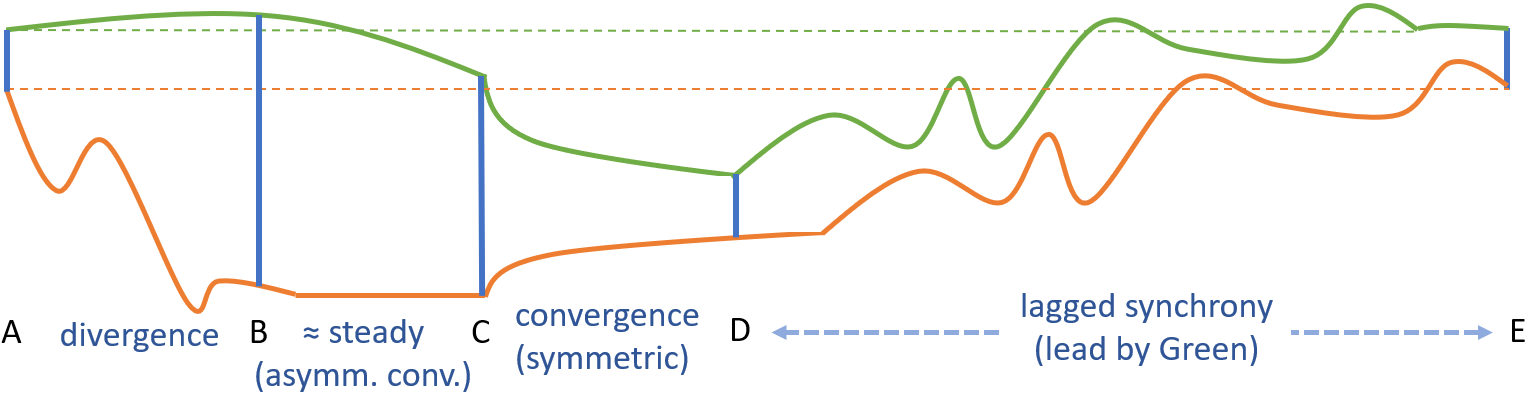
\includegraphics[width=\linewidth]{accommodation_types}
	\caption[Different accommodation types in a conversation]
		{The evolution of a feature's values produced by two speakers represented by the green and orange solid lines.
		The dashed lines connect the corresponding initial and final values of each speaker.
		The letters A to E mark timestamps with behavioral changes.
		Each caption describes the behavior between the two corresponding marks.}
	\label{fig:accommodation_types}
\end{figure}

\section{Vocal accommodation in human-computer interaction}
\label{sec:phonetic_convergence_in_hci}

%\subsection{What is an interaction?}
%\label{subsec:what_is_an_interaction}

\subsection{Verbal interaction with computers}
\label{subsec:verbal_interaction}

A \acf{hhi} is a mutual or reciprocal relationship between two (or more) interlocutors within a defined timespan.
This is also true for interaction with machines, though the beneficial side is typically the human speaker(s) while the machine is used to achieve the humans' goal.
In more modern applications, and especially when \ac{ai} is involved, the computer might also be programmed to \enquote{benefit} from the interaction, e.g., by acquiring information for future interactions or being able to finish a task more efficiently.
One type of interaction is a \emph{conversation}, where the communication is language-based.
This difference is more prominent in \ac{hci}, since there are ways to interact with machines without using written or spoken words, like using touchscreens, a computer mouse, or hand gestures. This can be compared to non-verbal -- neither written nor spoken -- human communication, but purely non-verbal communication occurs more often with machines than with people.
The main reason for that is probably since machines are not, yet, capable of using language as freely and verbosely as humans.
The terms \enquote{interaction} and \enquote{conversation} are often used interchangeably in this work, since the interactions in question are spoken conversations.
Nevertheless, interactions refer to a more general concept of communication that might involve other components than speech and conversations focus on the language components of the communication.
% spoken interaction -- Although the linguistic content might remain the same, adds complexity due to variety or speech and the technological challenge of generating inteligble speech output.

Interestingly, humans almost always need to compromise on the way they interact with computers or learn new interfaces (like those mentioned above) even for performing simple tasks.
Even in the case of spoken communication, which develops early on in humans, compromises need to be made as to how to speak to the computer so that it understands that user's intention.
For any of the system types mentioned in \cref{sec:types_of_sdss}, users need to learn how to modify their speech so that they can properly use the systems (be it the speech style of wording), instead of the system being able to adapt to the user.
With the advance of speech technology, this gap is shrinking, but there is still a way to go before computers will be able to understand and produce spoken language well enough so that people can speak to computers as they speak to other human beings.
The topics of this work capitalize on this evolution, to see whether \ac{hhi} phenomena like vocal accommodation are transferred to \ac{hci} as talking to computers becomes easier and more common.
More generally, the question rises whether \ac{cat} holds for \ac{hci} as well.
This is supported, for example, by the \ac{casa} paradigm \citep{Nass1994computers, Nass2000machines},
\todo{other places where CASA can be mentioned? definitely in General Discussion}
which argues that humans apply similar social behaviors when interacting with computers because they ascribe human characteristics to them.
As a starting point, domain-specific systems with alternate turn-taking are easier for computers, as they take away a lot of the complexity of spoken language and reduce it to individual utterances that can be mapped to actions the system supports.
For example, a \ac{sds} for ordering train tickets will probably follow a very specific protocol and react only to a specific input, as opposed, for example, for a general-purpose system that could talk with the user about a planned trip and help booking tickets as part of a longer, general-purpose conversation (see \cref{tab:sds_types}).

\subsection{Previous work}
\label{subsec:previous_work}

\todo{better title for this section?}

\Cref{sec:linguistic_accommodation} discusses vocal accommodation in \ac{hhi}, but this phenomenon has been studied in \ac{hci} as well.
A key difference between the two settings is the lack of naturalness on the computer's side. 
Since accommodation is often ascribed to mutual social aspects (as explained by \ac{cat} in \cref{sec:communication_accommodation_theory}), this introduces a limitation in the amount of accommodation that may occur.
Two main approaches are used to overcome this limitation in experiments:
Simulating a computer's output in a wizard-of-Oz setting and integrating some accommodation capabilities into a \ac{sds}.
Wizard-of-Oz experiments have the advantage that the output of the computer-based interlocutor can be directly controlled by the experimenter, usually using pre-defined utterances.
This grants precision and control over the experiment, which makes it a very suitable approach for research.
However, preparing the experimenter's control interface and the utterances might be time-consuming, e.g., if they need to be recorded or manually manipulated in a certain way.
Another disadvantage is the disability to deviate from a pre-defined script covered by the prepared utterances, limiting the variety of interactions the simulated system can support.
\Acp{sds} that support at least some level of accommodation or real-time manipulation save the time and effort of creating stimuli prior to the experiment.
Though the quality of the output and the time required to generate it might be affected, this setting better represents real-world \ac{hci} and can typically better react to varying paths the experiment is going (depending on its domain constraints).
As with real-world systems, it requires a lot of time to develop these capabilities, which often makes this option impractical in research.
\Cref{sec:adaptive_spoken_dialogue_systems} discusses further facets and possible solutions for integrating accommodation capabilities into \acp{sds}.

Using these two methods, various experiments have been conducted to measure accommodation in \ac{hci}.
%Various studies have investigated entrainment and priming in \acp{sds}, aiming to better understand \ac{hci} dynamics and improve task-completion rates.
\citet{Bergqvist2020nontrivial, Lopes2011primes}, for example, focused on dynamic entrainment and adaptation on the lexical level and found that users adapt to a system's terminology that differs from theirs.
This also led to improved performance in the given tasks.
\citet{Parent2010lexical} examined the correlation between lexical choices and word frequency using the \emph{Let's Go}~\ac{sds} \citep{Raux2005letsgo} and found that users adapt more to words that occur more often.
While these studies addressed the changes in experimental, scripted scenarios, the theoretical foundations for studying these changes in spontaneous dialogue exist as well \citep{Brennan1996lexical}.
\citet{Gasic2013policy, Levin2000stochastic} provide examples of online adaptation for dialogue policies and strategies.
Noticeably, while all of the studies mentioned above examine various facets of dialogues, none of those are related to the auditory aspects of speech -- the primary modality used to interact with \acp{sds}.
\citet{Benus2018prosodic} found relationships between the level of users' trust toward an avatar and the degree of the system's vocal entrainment or disentrainment.
Similarly, \citet[][pp.~142-144]{Levitan2014acoustic} shows relationships between prosodic entrainment and how much participants liked the avatar they were interacting with.
\citet{Bell2003prosodic} found that users' speech rate can be manipulated using a human-simulated \ac{sds}.
Similar results were found when intensity changes in children's interaction with synthesized output were examined \citep{Coulston2002amplitude}.
All these experiments focus on \ac{hci}, while those in \cref{sec:linguistic_accommodation} concentrate on \ac{hhi}.
However, accommodation in \ac{hhi} and \ac{hci} has not been directly compared within the same interaction, as done in \cref{chap:speech_variations_in_hhci}.
Furthermore, mainly suprasegmental characteristics have been studied for accommodation in \ac{hci}, mostly due to technical limitations (see \cref{sec:adaptive_spoken_dialogue_systems} for details).
A wizard-of-Oz experiment with a focus on \emph{segmental} features is described in \cref{chap:shadowing_experiment_with_natural_and_synthetic_voices}.
\chapter{Spoken Dialogue Systems}
\label{chap:spoken_dialogue_systems}

\lettrine{T}{his} chapter gives an overview on the \aclp{sds}, including common architectures, different system types, and implementation techniques.
The concept of adaptive \aclp{sds}, which is a core idea in this work, is introduced as well, along with the challenges involved and examples of possible adaptation strategies on different levels.

\pagebreak

%\section{What is a spoken dialogue system?}
%\label{sec:what_is_a_sds}
%\todo[inline]{here talk about what is a dialogue, a spoken dialogue, turn, when an interaction becomes a dialogue (is every interaction with a machine is a dialogue system?), etc. can really use the introductions given by Olga in the SDS seminar}

\noindent
\Acfp{sds} offer a wide range of services and are used in various forms every day both for commercial and personal purposes.
The main difference between them and many other ways to communicate with computers is the use of speech -- and mostly speech alone -- for interaction.
This offers benefits to the users, like begin able to perform tasks while keeping their hands free, contrary to systems that require textual input from a keyboard or haptic touch on a screen.
We are witnessing an ever-growing presence of voice-activated devices, like speech-activated cars, hands-free medical assistants, and \acp{its}.
These devices support more and more functionalities in a way that is more comfortable and intuitive for users.
It can be expected that in the near future such devices will be used not only by individuals, but also in more social contexts, including interactions where multiple humans are involved.
This makes the understanding and improvement of social skills in \acp{sds} all the more important.

The common architecture of \acp{sds} is explained in \cref{sec:architecture_sds}, along with details about each component and free tools for building them.
\Cref{sec:types_of_sdss} gives an overview of an application that uses a \ac{sds} to communicate with users.
A roadmap toward \acp{sds} with vocal accommodation capabilities as well as the challenges involved are discussed in \cref{sec:adaptive_spoken_dialogue_systems}.
Such capabilities would improve the personalization and overall experience of the interaction.

\section{Architecture of \aclp{sds}}
\label{sec:architecture_sds}

As shown in \cref{fig:sds_architecture}, the architecture is symmetric in terms of input and output types.
Each cycle starts and ends with speech signals, generated first by the user, and then by the system (a more sophisticated system can also take the initiative).
The content of the utterance, usually referred to as \emph{intent}, is then extracted to determine its objective.
Similarly, the system's speech output is based on generated content that captures some intent.
The \enquote{brain} at the core of the cycle decides what intent is most suitable for the user's input.
This may be done purely by learning from provided dialogue examples, with the help of external information or databases, based on hand-crafted rules, or some combination of those.
This simplified flow assumes that the user and the system take turns alternately, one at a time.
However, one interlocutor may of course needs multiple consecutive turns to convey the message due to length or no response from the other.
Although each component is a whole research area by itself, there are numerous open-source implementations that help to quickly build a basic \ac{e2e} system and focus on a specific one.
Brief overviews of these \ac{nlp} tasks are given in \crefrange{subsec:automatic_speech_recognition}{subsec:text-to-speech_synthesis}.
Note that this is a basic typical architecture and each component may be extended or modified.
Specifically, this architecture changes substantially in fully neural-based systems.
However, even in that case, the general flow (and by extension the training data) remain the same.
%
\begin{figure}[t]
	\centering
	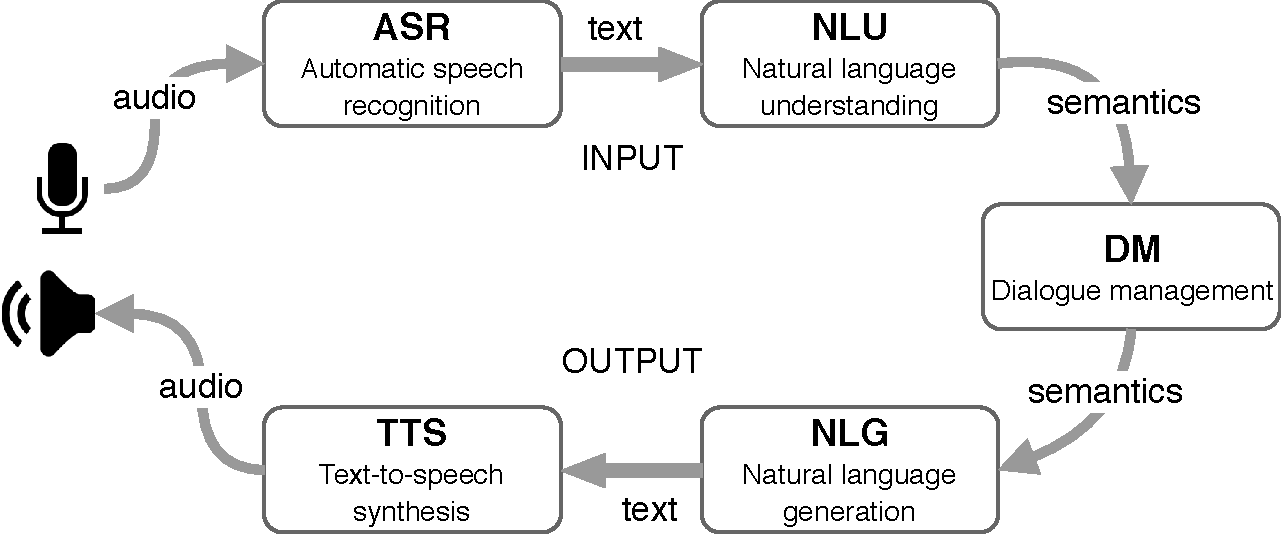
\includegraphics[width=\linewidth]{sds_architecture}
	\caption[Architecture of a spoken dialogue system]
	{A typical architecture of a spoken dialogue system.
	The interaction lifecycle is symmetric, and for each analysis input step there is a corresponding generation output step.
	The exchange usually starts with a user spoken utterance and ends with the system's spoken response.}
	\label{fig:sds_architecture}
\end{figure}

\subsection{\Acl{asr}}
\label{subsec:automatic_speech_recognition}

An essential condition for verbal communication is to be able to hear what the interlocutor says and process it into words.
For computer, this is done using \acf{asr}, which transfers the audio signals produced by the user's articulators into some machine-readable form that can subsequently be fed to the \ac{nlu} component.
This step is crucial for vocal accommodation, as it the only component that accesses the audio signal.
However, \acp{sds} predominantly merely use it to extract the said words and discard it afterwards.
As a result, they know \emph{what} was said by the user (subjected to the quality of the \ac{asr}) but not \emph{how} it was said.
For any kind of responsive behavior, this component must be extended to provide some additional information about the input speech.

\subsubsection{Tools}
\label{subsubsec:tools_asr}

Kaldi \citep{Povey2011kaldi} and CMU Sphinx \citep{Lamere2003sphinx} are free-to-use \ac{asr} engines that offer various functionalities, including training a model on a custom dataset.
For the purpose of vocal accommodation, one benefit of using such modifiable toolkits is the ability to access the phoneme times.
This is crucial for detecting and tracking certain phonetic features, and segmental ones in particular (see \cref{chap:convergence_module_for_sdss} for utilization of this).

\subsection{\Acl{nlu}}
\label{subsec:natural_language_understanding}

After getting the words spoken by the user, the system needs to infer an intention from them, i.e., what the user wants to achieve in this turn.
This is the role of the \acf{nlu} component.
An intention can be as simple as asking the \ac{sds} to perform a task (e.g., to turn on the radio in a voice-activated car).
such requests are mostly recognizable by pre-defined keywords the system can look for in the transcribed input text.
Other requests, like inquiring information about a place or booking a flight, require the system to be able to withdraw -- and properly formulate -- information from some source.
Such tasks require further information (e.g., flight origin and destination, date, price range, etc.) to be completed, or, if said information not provided by the user, additional turns where the system asks for the missing bits.
This process is called slot-filling.
\putref{need example reference for slot filling?}
More complex reactions, and especially in the case of chatbots, demands deeper semantic analysis, as the intention might not be explicitly articulated and in some cases, such a defined intention may not even exist.

%\subsubsection{Tools}
%\label{subsubsec:tools_nlu}

\subsection{\Acl{dm}}
\label{subsec:dialogue_management}

After completing processing the user's input, a decision must be made by the \ac{sds} as to how to react.
This is done by the \acf{dm}, which is the central component of a \ac{sds}.
The \ac{dm} is typically divided into \emph{belief tracker} and \emph{policy} modules.
The former accumulates information regarding the user's wish based on current and previous turns, while the latter is responsible for determining the most appropriate response to that intention.
If any additional data is required for satisfying the user's needs, e.g., some information from the web or a database, the retrieval will be done by the \ac{dm}.
The same goes for specific domain knowledge, which can be made available to the system as part of its implementation.
Deciding on the best action can be achieved using a deterministic rule system for a small number of simple cases (a \ac{cnc} system, for example), but need more sophisticated models for more involved situations.
One commonly used technique is reinforcement learning, which is suitable for making selecting an action based on a given state (the \enquote{environment}).
All these conditions determine how flexible and elaborate the system is, and specifically how large is the domain -- or domains -- it can handle.

\putref{references for rule-based system, RL-based system (Milica?), and adapting DM (add sentence about that at the end)}

\todo[inline]{if it helps, can add a graph like the one from Milica's slide: breadth vs.\ depth of domain in SDS (variety vs.\ complexity). replicate the graph Milica showed in her talk (x-axis is breadth and y-axis depth, with some examples along combinations of the axes.}

%\subsubsection{Tools}
%\label{subsubsec:tools_dm}

\subsection{\Acl{nlg}}
\label{subsec:natural_language_generation}

After deciding on the most appropriate response to the user, the system needs to convey it in a human-understandable manner, namely words.
The process is reversed to \ac{nlg}, i.e., generating text based on a certain intent.
Depending on the user's input intent, the system may respond with simple acknowledgment statements, repetition and information approval, or completely newly formed full sentences.
Additional challenges of this task often root from things that could be reduced or ignored in \ac{nlu}, but must be precise in \ac{nlg}.
For example, using wrong verb conjugations and tenses will cause the system's response to sound ungrammatical or ill-formed in some cases, but could even convey a different message.
therefore, depending on the language, the \ac{nlg} component should there be aware to the user's gender, the number of users speaking to it, the nature of the user's intent and how it may be carried out, and more (in multimodal systems, these would influence other modalities, like gaze, as well).

%\subsubsection{Tools}
%\label{subsubsec:tools_nlg}

\subsection{\Acl{tts} synthesis}
\label{subsec:text-to-speech_synthesis}

The last step in the flow is converting the text provided by the \ac{nlg} component to speech signal and play it to the user.
This is done using a \acf{tts} module, which takes orthographic forms of words and outputs a voice that utters them.
Unlike some older methods, nowadays voices are learned from recorded human speech, by selecting and concatenating small units of it.
Linguistic analyses are performed to translate the orthographic forms to sound sequences, insert stresses and pauses, etc.
Additional properties, like the contour and duration, are typically determined in inference time.
Newer methods are mostly neural-based and can generate audio frames directly from text \citep{Shen2018natural}.
All these methods have the limitation of not being able to control the generation process directly, especially not on the segmental level.
This makes it hard to apply detected changes in the user's speech, which is a major barrier on the way to integrate accommodation capabilities into \acp{sds}.
Nevertheless, there are examples of \acp{sds} that can adapt on various levels, including specific modifications in speech (see \cref{sec:adaptive_spoken_dialogue_systems}).

\subsubsection{Tools}
\label{subsubsec:tools_tts}

Free \ac{tts} engines for training voices include Festival \citep{Black1997festival}, espeak \citep{Duddington2012espeak}, and MaryTTS \citep{Schroder2011open}.
In addition to being used as \ac{e2e} \ac{tts} pipelines, these systems can also provide intermediate analysis outputs like phonetic transcriptions.

\section{Types of \aclp{sds}}
\label{sec:types_of_sdss}

By and large, \acp{sds} can be divided into two main categories, which determine the communication style and behavior of the system: task-oriented systems \citep[e.g.,][]{Wen2016network, Zhao2016towards} and chatbots systems \citep[e.g.,][]{Vinyals2015neural, Li2016deep}.
\Cref{tab:sds_types} compares these two main categories.
Vocal accommodation is relevant for both these system categories, but in different ways.
Task-oriented systems may need to accommodate faster and potentially introduce changes on every turn, leading to sharper, possibly unpleasant changes.
It might also be required to reset the system's speech for each interaction if it's used by more than one user or for different purposes.
Chatbots, on the other hand, might be able to exploit the fact that they are usually involved in longer conversations, giving them more time to learn the user's speech.
This could lead to a slower, smoother, and probably less apparent process, which should gradually improve the personalization of the system.
Another category is voice-activated \ac{cnc} systems, which are arguably not \acp{sds} per se, since they only rarely engage in conversation  or trigger a multi-turn dialogue.
Therefore, such systems do not leave any room for accommodation to occur.
Nevertheless, \ac{cnc} systems are considered a simple kind of task-oriented \ac{sds} in this work, as ultimately they are designed to achieve a specific task, even if a dialogue is not necessarily required for that.
Indeed, task-oriented systems like \acp{pa} often offer \ac{cnc} commands as well.
\Acp{sds} can be utilized in various ways and be embedded in different types of systems.
\Crefrange{subsec:personal_assistants}{subsec:virtual_humans} survey some of the main system types with a \ac{sds} at their core.
%
\begin{table}[tb]
	\centering
	\caption[Types of \aclp{sds}: Task-oriented vs.\ Chatbots]{A comparison of some characteristics in task-oriented \acp{sds} and chatbots.}
	\label{tab:sds_types}
	\begin{tabularx}{\linewidth}{>{\bfseries}lp{.38\linewidth}p{.37\linewidth}}
		\toprule
		\vspace{.3cm}
							& \multicolumn{1}{c}{{\large \textbf{Task-oriented}}} & \multicolumn{1}{c}{{\large \textbf{Chatbots}}} \\
		\vspace{.2cm}
		Goal				& Help the user achieve a specific, pre-defined goal
							& Converse as naturally and continuously as possible \\
		\vspace{.2cm}
		Applications		& \Aclp{pa}, \ac{cnc} systems, in-car voice-activated systems, reservations, etc.
							& Free-form \acl{c-ai} applications: chitchat bots, social robots, etc. \\
		\vspace{.2cm}
		Domain				& Domain-specific and/or multi-domain
							& Domain-free or robust within-domain \\
		\vspace{.2cm}
		Modeling			& Statistical models and/or handcrafted rules
							& Typically \ac{s2s} models with no-go filters \\
		\vspace{.2cm}
		Evaluation			& Task completion rate and completion time, number of turns (+ subjective criteria)
							& Chat length, relevant replies ratio, user engagement, general user satisfaction \\
		\bottomrule
	\end{tabularx}
\end{table}
%
\subsection{\Aclp{pa}}
\label{subsec:personal_assistants}

A \acl{pa} (\acs{pa}; frequently also \emph{intelligent \acl{pa}} or \emph{virtual \acl{pa}}\footnote{The term \emph{virtual assistant} is widely used as well. However, it is avoided here, since it also refers to a different kind of occupation (\url{https://www.investopedia.com/terms/v/virtual-assistant.asp}).}) is a software-based program (sometimes embedded into a dedicated device (see \cref{subsec:smart_speakers}) that in some way fills the role of a human-being personal assistant.
More often than not this includes mainly straightforward tasks the latter can perform, like managing schedules and tasks, but the support for more complex tasks is rapidly increasing and nowadays may also include in-context question answering, smart online shopping, and more.
An advantage of \acp{pa} is their simple operation, which is almost exclusively voice-based, making them accessible to the general public.
Commercial voiced-based \acp{pa} include Amazon Alexa, Apple Siri, Google Assistant, Microsoft Cortana, and many other, less famous ones.

Besides making the operation of such voice-activated systems simple and user-friendly, \acp{pa} also aim to let users interact with them in a familiar, natural manner.
One property of natural interactions is the tendency to accommodate to the specific situation and interlocutors to make the interactions more fluent and efficient \citep{Gallois2015CAT}.
Linguistic accommodation is one aspect of this phenomenon, and it is found in various \ac{hhi} experiments \citep[e.g.,][]{Pardo2017phonetic,Schweitzer2017social}.
\Cref{chap:speech_variations_in_hhci} presents a study of vocal accommodation in multiparty interactions with a \ac{pa}.

In recent years, the market for commercial \acp{pa} has grown rapidly.
For example, Microsoft Cortana had 133 million active users in 2016 \citep{Osborne2016why} and Echo Dot was Amazon's best-selling product between 2016 and 2018 \citep{Dickey2017echo}.
Furthermore, \SI{72}{\percent} of people who own a smart speaker say they often use their devices as part of their daily routine \citep{Kleinberg2018ways}.

\subsection{Smart speakers}
\label{subsec:smart_speakers}

Smart speakers (or \emph{intelligent speakers}) are small loudspeakers typically used by one to several users in a common household or working environment.
The speakers themselves merely offer audio transmission with some basic, hands-free operation.
The \enquote{smart} portion comes from the software installed on it, which is usually some variety of a \ac{pa} (see \cref{subsec:personal_assistants}).
Mainstream smart speakers device series (and the \ac{pa} powering them) include Amazon Echo (Alexa), Apple HomePod (Siri), Google Home (Google Assistant), and Microsoft Invoke (Cortana).
Newer devices, called \emph{smart displays}, can also be operated via a touchscreen.
Their easy operation and the convenience they offer make smart speakers very popular with steadily increasing user base, with some estimations of more than 150 million units sold in the United States alone by the beginning of 2020\footnote{\url{https://marketingland.com/more-than-200-million-smart-speakers-have-been-sold-why-arent-they-a-marketing-channel-276012}} and a rapidly increasing usage in other countries\footnote{\url{https://www.emarketer.com/content/global-smart-speaker-users-2019}}.

\subsection{Chatbots}
\label{subsec:chatbots}

Chatbots (a.k.a.\ \emph{chatterbots} and \emph{chitchat bots}) are conversational agents that do not aim to accomplish a specific in-domain task, but to create a human-like communication with the user in lieu of a real human interlocutor.
This makes the scope and evaluation of a chatbot more complex, as the definition of the end-goal is not as well-defined (and cf.\ \cref{tab:sds_types}).
Due to their nature, chatbots can be utilized in a variety of ways, and are usually embedded in social robots, virtual agents, or smart speakers that offer one as a separate functionality.

An early example of a program considered a chatbot with a defined purpose is ELIZA \citep{Weizenbaum1966eliza}, which tried to imitate the role of a therapist in a therapeutic session.
While ELIZA's functionality can, for the most part, be reduced to simple word matching, it was revolutionary for the time and open the way to more sophisticated methods.
Nowadays, chatbots are used for improving experience and service in online customer support and instant messaging apps.
Nowadays, chatbots have already been used in various domains, such as education \citep{Benotti2014engaging, Kerly2007bringing}, elderly care \citep{Iio2020twin}, cultural heritage \citep{Pilato2005expert}, healthcare \citep{Kowatsch2017text}, software development \citep{Lebeuf2017software}, and others \citep{Shawar2007chatbots}.

\subsection{Embodied agents and social robots}
\label{subsec:embodied_agents}

Embodied agents (sometimes also \emph{interface agents}) are communicative systems with some visual form.
Though the embodiment may be graphical only (see \cref{subsec:virtual_humans}, this term usually refers to systems that interact and communicate with the environment through some physical shape.
For social robots, this shape is normally human-like and may include a full-body representation (like the NAO robot \citep{Singh2016nao}) or only a face (like Furhat \citep{AlMoubayed2012furhat}).
Social robots gather information in different modalities, like eye gaze and hand gestures, and may even generate some limited behavior in these modalities, but ultimately their primary means of communication is almost always speech.
Accommodation towards embodied interlocutors is especially interesting, as it is closest to face-to-face \ac{hhi}.
Vocal accommodation has been found in human-robot interaction, e.g., by \citet{Ibrahim2019fundamental}.

\todo[inline]{would it bring any added value to put an image of interaction with NAO and/or Furhat?}

\subsection{Virtual humans and avatars}
\label{subsec:virtual_humans}

Though commonly used interchangeably in the literature, \acp{vh} and avatars refer to two similar yet distinct concepts.
On-screen representations of an interlocutor (sometimes of the user) are largely referred to as \emph{avatars}.
Those can be static images associated with specific speakers,\putref{put Michelle's Interspeech 2020 paper as an example if accepted} but nowadays normally include at least some basic facial expressions and animations.
In addition, avatars are also used sometimes as a general term for any virtual, graphically rendered interlocutor (including a \ac{vh}).
\Acp{vh}, on the other hand, are fully depicted humanoids that aim to portray a real human being as closely as possible.
This typically entails characters with full bodies, but partial figures are used as well, depending on the application.
Similar to agents with a physical embodiment (\cref{subsec:embodied_agents}), these conversational agents are capable  of multimodal communication.
They can be used in various interactive activities, like language assessment \citep{Peterson2005learning} and therapy \citep{Devault2014simsensei}.
Experiments have shown vocal accommodation effects in interactions with \acp{vh} with respect to features like speech rate and \ac{f0} \citep{Gijssels2016speech, Staum2010virtually}.

\section{Accommodative spoken dialogue systems}
\label{sec:adaptive_spoken_dialogue_systems}

Dynamically changing the voice is a capability currently ascribed almost exclusively to humans and exist only sparsely and simplistically in computer-based systems.
A voice-activated device always talks the same way, regardless of how the user speaks to it, the environment and setting in which the interaction takes place, the goal and role of the device, etc.
This capability, which comes naturally to humans in social interactions, involves several steps of (partially unaware) decisions, which together form the overall effect of becoming behaviorally more or less similar to an interlocutor, as explained in \cref{sec:communication_accommodation_theory}.
These include both situational and knowledge-related facets like how it is expected to behave in certain situations and which vocal changes fit those, as well as the physiological ability to apply these matches.
Humans can perform all of these steps as one conduct.
For computers, however, these steps must be broken down and \emph{explained}, as they lack such common social background knowledge and the intuition as for how to match their voice to the situation.
Several attempts to integrate this capability into \acp{sds} are presented below, followed by a description of a roadmap toward such a system and an introduction of relevant terminology to describe these different steps and ways to achieve accommodative vocal behavior in machines.
The parallelisms to the human perspective are highlighted along the way to help to understand the motivations and goals.

\todo[inline]{here take 2-3 systems (from Chapter 1 and/or 3) and explain a bit in detail how they implemented the accommodation capabilities. specifically, emphasize the limitations and hint how the work here is doing more}

%Studying convergence in speech in an \ac{hci} context is made possible with more natural synthesis technology, which gives more fine-grained control over parameters of the system's spoken output.

% A technical overview of the development of adaptive \acp{sds} is given by \citet{Levitan2016implementing}, where speech rate and intensity are entrained by the system.

\subsection{Roadmap and challenges}
\label{subsec:roadmap_and_challenges}

\subsubsection{Dialogue is hard}
\label{subsubsec:dialogue_is_hard}

\citep{Turing1950computing}\ldots

\subsubsection{Suggested roadmap}
\label{subsubsec:suggested roadmap}

The lack of accommodative speech in computer-based systems roots from what is more often than not natural and even automatic for humans, namely realizing how and how much to change their vocal behavior, the physiological means to express those differences, and the ability to combine the two into a coherent production in an interaction.
\Cref{fig:roadmap_adaptive_sds} shows an overview of a (simplified) roadmap to integrating adaptive capabilities into a \ac{sds}.
In addition to the expected functionalities of a standard \ac{sds}, three main elements are required:
For one thing, knowledge about the nature and properties of accommodative behaviors in humans is required.
This includes both empiric experimental data and integrable models.
% 1-2 sentence that at the moment there are many ways to measure accommodation and existing models are limited (reference? or at least point to terminology part)
Furthermore, the technical capability to control the speech output on demand is essential for introducing flexibility in the system's base voice.
This also includes a mechanism for accumulating phonetic evidence from the user's input relevant for the feature representations used for the accommodation process.
As these manipulations must be applied in real-time, re-training the \ac{tts} model to capture every change is not only insufficient, but not practical as well.
This means that the manipulations are done on top of the existing \ac{tts} model, either by modifying the outputted waveform directly or by training a model that can take specific changes in feature description into consideration.
\putref{if chapter about those methods comes to life, refer to them}
To link between the modeled theoretical knowledge and the audio processing engineering implementations, an additional component must be introduced in the system.
The role of this component is to feed the system's flexible voice parameters result from the models to express vocal changes, which are ultimately conveyed to the user.
This emphasizes the notion of the \ac{nlg} module decides \emph{what} the system says while the \ac{tts} module determines \emph{how} it will say it.
This is further explained and illustrated in \cref{chap:convergence_module_for_sdss,fig:adaptation_module_architecture}.

This work addresses each of those facets.
\putref{when parts are more final, briefly refer to them here}
These aspects make the task of integrating flexible vocal characteristics into \acp{sds} an involved task, each with its own challenges that requires a profound work to investigate.
%
\begin{figure}[t]
	\centering
	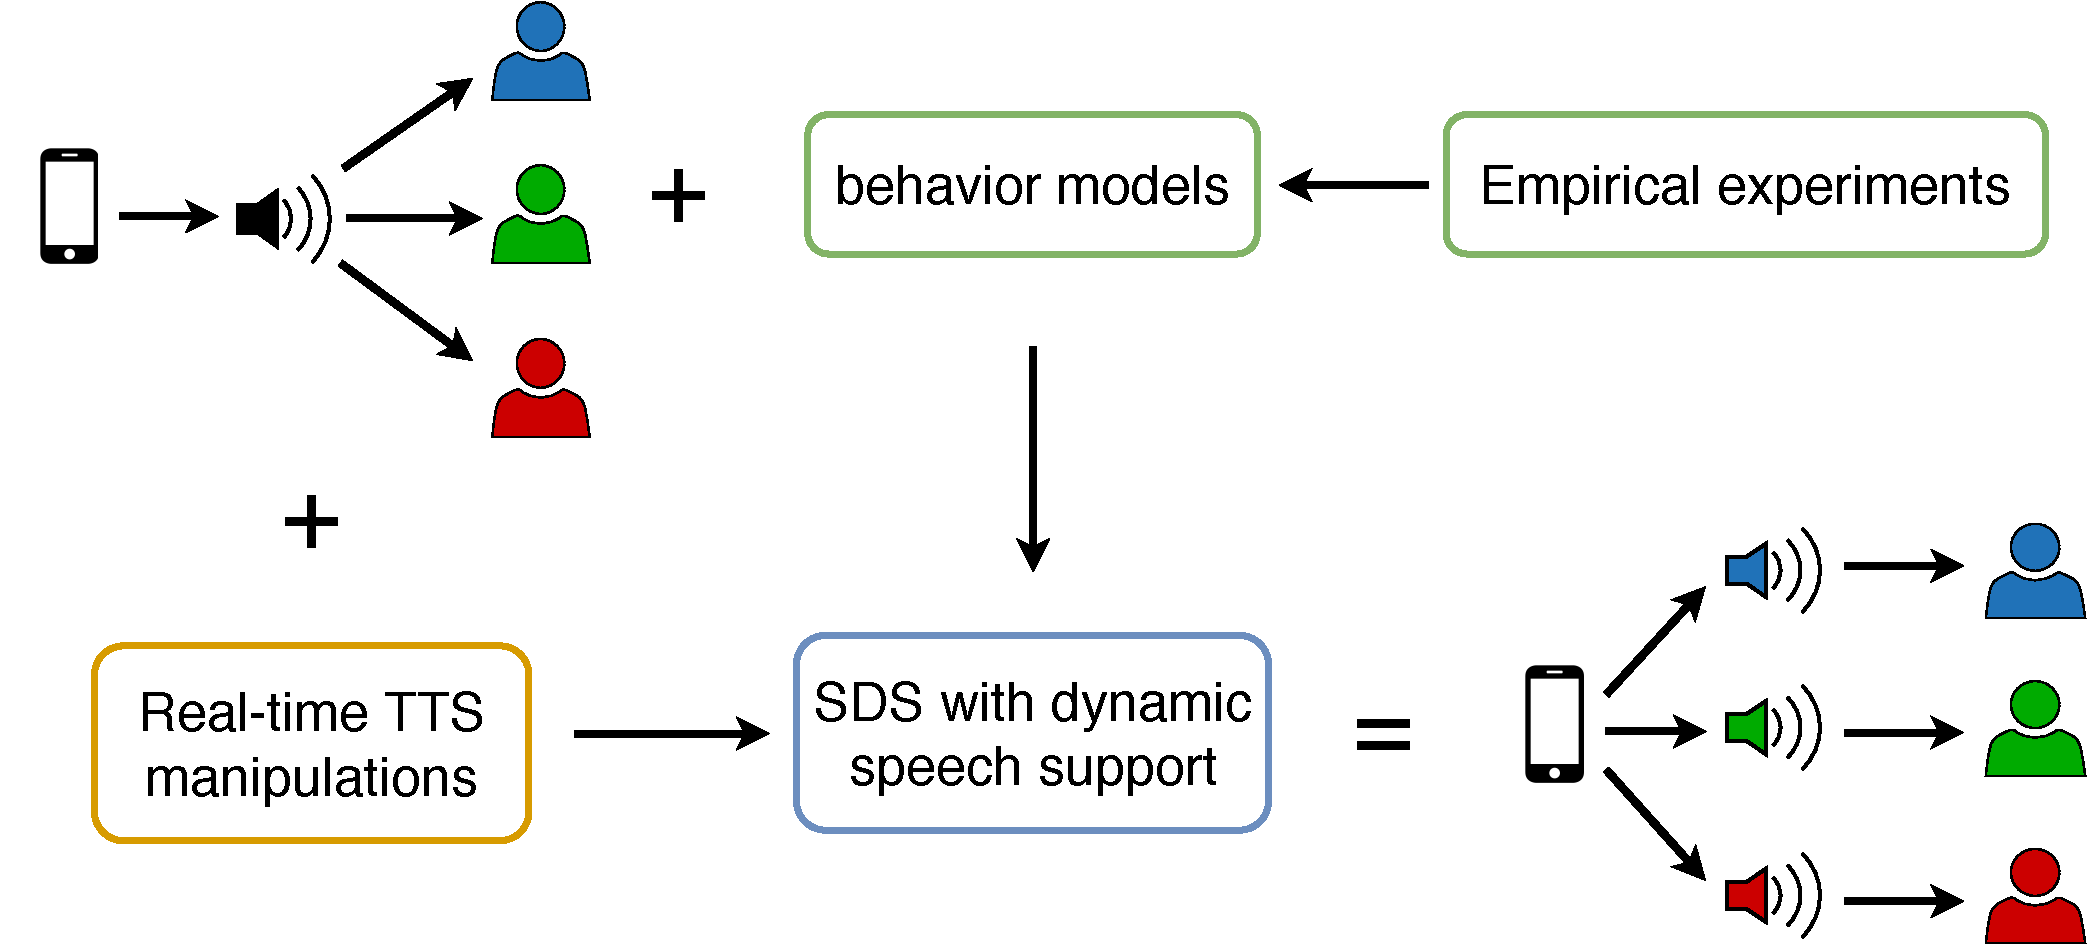
\includegraphics[width=\linewidth]{roadmap_adaptive_sds}
	\caption[Roadmap to phonetically adaptive \acl{sds}]
		{A suggested roadmap from static outputs (top left) to personalized outputs (bottom right) in \acp{sds} (and see \cref{fig:output_not_adapted,fig:output_adapted}).
		The green, orange, and blue blocks stand for the modeling, manipulation, and integration components described in the text, respectively.
		The \enquote*{+} signs represent direct addition to a static system and the arrows go from components required as a feed to others.}
	\label{fig:roadmap_adaptive_sds}
\end{figure}
%
For a \ac{sds} to accommodate with its speech, it would not only need to support dynamic, on-demand changes of its \ac{tts} component's output, but would also need its \ac{asr} component to be able to identify and track specific features in the user's speech to update its representation of those features.
Completing the cycle, these representations can then be used as additional input for the \ac{tts} components to determine how those would influence the system's speech output.
This process is individual for each speaker (see \cref{fig:static_vs_adaptive_speech_output}) and may occur over long periods of time or multiple interactions, depending on the desired degree and characteristics of accommodation.
Furthermore, this process may involve other components of the \ac{sds} as well (cf.\ \cref{fig:sds_architecture}).
For instance, the Dialogue Manager might consider changes in the user's speech when making decisions, e.g., based on apparent mood and calmness.
The \ac{nlg} component could make alterations to its output to better fit the vocal changes of the system and the user's dynamic state, such as shortening sentences and omit additional information if phonetic indicators of hurry or urgency (like those shown by \citet{Edworthy2003acoustic}) are detected in the speech input.

\subsection{Terminology -- accommodation levels}
\label{subsec:accommodation_levels}

In addition to all the above, another design choice for accommodative \acp{sds}, which is not explicitly required in human speech, concerns the overall \emph{level of accommodation} the system introduces.
This determines the fundamental behavior and form of variation in the system's speech, regardless of specific phonetic features, utterance contents, etc.
The variation levels (or properties) described below can potentially be combined in different ways to achieve the desired system behavior.
They are, at least to some extent, analogous to aforementioned processes conducted by humans in social interactions, with the key difference that humans don't need to defined and think about them separately, if at all.
The utilization of these levels is demonstrated in the context of phonetic accommodation, which is one case of dynamic change of speech \citep[as in][to name a few]{Weise2019individual, Schweitzer2016exemplar, Bevnuvs2014social}.
\Cref{chap:web-based_responsive_spoken_dialogue_system} further discusses and demonstrates the integration of such properties into a \ac{sds}.

Different terms are used in the literature to describe systems that can change their output.
This often leads to inconsistencies and mix-ups in terminology.
Definitions of five core properties of accommodative \ac{tts} that should, once accomplished, grant a more dynamic appearance, along with their suggested use and potential fusion with one another, are suggested below.
These terms seek to distinguish between the different capabilities that can be integrated into \acp{sds} and the way they relate to humans’ behaviors and each other.
%
\begin{description}
	\item[Adaptive] -- the vocal behavior evolves between and/or during interactions.\\
	This property refers to the system's use of any mean to \emph{dynamically} change it speech-related behavior, regardless of the source of influence, the goal or direction, or specific realizations.
%	Here, adapting means shifting the overall behaviors by updating a subset of the other properties.
	That means, for example, modifying the base behavior, extending the variability, or reflecting the system's changes earlier.
	This can happen between interactions or within a single, usually longer, interaction.
	The former could be more useful for \ac{cnc} systems or goal-oriented \acp{sds} that are used by many users, while the latter is more suitable for social systems like chatbots and \acp{pa} (see \cref{sec:types_of_sdss}).
	Ultimately, this is a means for the system to improve its performance and accessibility based on previous interactions.
	However, for some applications, like a \ac{capt} system, for example, it would be better to \enquote{reset} their behavior between each use to offer a better experience.

	\item[Flexible] -- on-demand speech manipulation \emph{without rebuilding the voice}.\\
	This property refers to the \emph{technical capability} to alter the system's speech output on request, which is achieved either via modifications in the voice's representation and parameters or by manipulating the outputted waveform directly using signal processing methods.
	Note that this does not entail the way this capability is used, and especially not that it is applied automatically.
	Moreover, as mentioned above, the technical capability to control the voice alone is not enough to create an accommodative behavior.
	This would also require additional data to be transferred to the \ac{tts} component to determine what manipulation to perform.
	For that end, the modeling steps can be built on top of this technical ground.
	It is important to note that this property compensates for the inherent ability in humans to control their voice at will, and therefore does not directly represent any specific element of humans' speech behavior like the other properties.
	
	\item[Responsive] -- changes are influenced by some \emph{external} speech input.\\
	A responsive system can, for instance, detect some target features in the user's speech input and, after comparing them to the system's representation of these features, guide the \ac{tts} on how to update them (typically, to make them more similar to the user's input).
	This requires a computational model that performs these steps (cf.\ \cref{chap:computational_model}).
	Yet this model would not have an independently defined behavior and it could only directly become more similar (or dissimilar) to the user in some fashion.
	Such models can be designed to imitate the user's immediate output from previous turns (like in \citet{Levitan2016implementing}) or to gradually match it based on some parameters like sensitivity and interaction's history (as demonstrated in \citet{Raveh2017Interspeech}).
	This property represents the idea that humans change their speech (and behavior in general) when interacting with other people, which is a key aspect of the \ac{cat} \citep[][and see \cref{sec:communication_accommodation_theory}]{Giles1991CAT}.
	
	\item[Characterized (Profiled)] -- the system's voice has its own base behavior.\\
	Giving a \enquote{character} (or a \emph{profile}) to a voice means that it has a specified base behavior, which might include general properties of accommodation.
	This can also be seen as a \emph{role} the system plays in a conversation, e.g., if built based on a certain \ac{hhi} scenario \citep{Silber-Varod2018prosodic}.
	In that case, the system would try to stick to some pre-defined model, which contains the required information to fulfill said role.
	A system might also have several profiles to switch between based on the settings and goals of the interaction.
	In the context of accommodation, that would include, for example, the degree of accommodation, its timing, or how strongly the system will try to influence the user's speech.
	This property represents the fact that a human being has a certain -- however complex -- personality.
	More specifically, a vocal identity, which will be expressed in spoken interactions.
	This idea is the basis for the simulations presented \cref{chap:statistical_model}, where each generative model can be seen as a core behavior.
	
	\item[Variable] -- variations on top of the base behavior are yielded.\\
	Some variations can be introduced based on the base profile.
	These are relatively minor differences that deviate from the voice's characteristics or enhance them in some way.
	From a system's point of view, the main purpose of such variations is to make the output style non-deterministic and therefore less repetitive and predictable.
	From the human point of view, this coincides with the difficulty to reproduce identical utterances in exactly the same way every time.
	Moreover, people, though having their own individual personality, would speak differently based on various factors outside a conversation like their mood, the environmental conditions, time constraints, etc.
	This property comes, therefore, to grant some smaller-scale dynamics to the voice, in particular when its base behavior is deterministic.
	\Cref{chap:statistical_model} explains in details an approach to achieve such variational behaviors with examples provided in \cref{sec:clustering_and_incremental_generation,tab:generated_symbol_sequences}.
\end{description}
%

% ----------
% REVIEW: Only mention in case some statistical model is include in the thesis that deals with that (a time-series one or variational autoencoder). in that case briefly say what it means and refer to the relevant chapter

%This work concentrates on facets concerning the properties \emph{characterized} and \emph{variable}, which have been given little attention in \ac{sds} research.
%Together, these two properties results in a flexible, non-deterministic output derived from a defined core behavior (that might itself vary).
%Added to the responsive output creates a system that changes with respect to the user according to its own base behavior and probabilistic variations.
%The balance between the influences from the user input and the system's profile can be defined as well, similarly to the bias utilized in speech adaptation, in the form of \putref{reference to this method)}
%\todo{sentence about balance might be unnecessary}
% ----------

\subsection{Systems with accommodation capabilities}
\label{subsec:systems_with_accommodation_capabilities}

\citet{Levitan2016implementing} % the system that (linearly?) entraining. read the deatils again and then say how this differs from the architecture in this paper. also, find references there for more such systems.

\section{Evaluating spoken dialogue systems}
\label{sec:evaluation_of_sdss}

\todo[inline]{decide whether a section about evaluation is necessary}

\ldots Therefore, evaluation of \acp{sds} depends on the purpose of the systems, which can be divided into two types, namely \textit{\aclp{tds}} and \textit{\aclp{ngs}}.

\subsection{Task-driven Systems}
\label{subsec:task-driven_systems}
[doesn't really evaluate the \ac{sds}, but it's ability to predict what task should be performed]
[typically part of a bigger system (which has a set of tasks it can perform (e.g. personal assistant))]

\subsection{Non-goal Systems}
\label{subsec:non-goal_systems}

A \acf{ngs} is a \ac{sds} that does not necessarily aim to complete a specific task (unlike \acp{tds}).
Its purpose is, then, more general and there might not even be a defined purpose for it.
Chatbots (see \cref{subsec:chatbots}) are a good a example for a \ac{sds} that typically isn't used for accomplishing a practical task like getting information or operating a device.
Instead, they are used as a long-term social companion (be it at home or as part of a mobile device) and even merely for entertainment. \todo{references for both examples}
Since such systems don't help to achieve a defined goal, it is not possible to evaluate their performance based on how well (or whether at all) this goal task was carried out.
There is a need therefore for another, more long-term and interaction-oriented method rather than a task-oriented method.
On the one hand, from the \ac{hci} point of view, the advantage of such methods is that they evaluate the dialogue capabilities of the system and not merely it's ability to map speech patterns or keywords to a set pre-defined actions.
On the other hand, however, the problem in such methods is that it is much harder to define metrics when the goal of the interaction is not completely defined.
There are two approaches to solve this issue:
The first is defining the 


\part{Experiments}
\label{part:experiments}

\chapter{Vocal Accommodation in Real-World Sales Calls}
\label{chap:conv_analysis}

\lettrine{H}{uman}-human interaction is an essential part of sales representatives' everyday work.
Controlling their communication skills is key for their deal to be successful.
The role of vocal accommodation in measuring and improving said skills is presented here as part of the greater concept of \acl{c-iq}.
Non-linear analyses methods are used to examine mutual influences in a collection of real-world high-stake sales calls.

\pagebreak

\section{Speech alignment for conversation intelligence}
\label{sec:conversation_intelligence}

Sales leaders have always been impelled to be able to reason why some of their representatives -- henceforth \emph{reps} or \emph{\acp{ae}} -- consistently attain, or even exceed, their goals while others do not \citep[see overview in][]{Kovac2017its}.
Yet, sales executives rely on data that is inherently flawed, as it is based on reports from sources like \ac{crm} systems.
Such systems only contain \enquote{dry} details regarding the stage the deals are in along with high-level numeric data and some, often subjective, estimations regarding the next steps.
That leaves the executives in the dark about the happenings at the front lines and the small-scale, day-to-day conducts and modi operandi that are decisive for the success of the \acp{ae}.
As a result, the reasons for losing or winning a deal often remain a riddle, making sales seem like an art based on anecdotes rather than a scientifically explainable practice \citep{Yohn2016best, Martin2017six}.
In his seminal book, \citet{Gladwell2006tipping} writes that \textquote[p.\ 83]{Part of what it means to have a persuasive personality is that you can draw others into your own rhythms and dictate the terms of the interaction}.
Supporting that, \citet{Orlob2018nine} found that star reps\footnote{Sales representative whose performances (and specifically their closed-deals rate) are often refer to as \emph{star reps}.The specific criteria are typically include a wide range of behavioral and business metrics, but those are decided internally per company and do not have an absolute definition.} are able to make prospects increase their speaking rate to match theirs, bringing the two sides closer with respect to this phonetic feature.
However, the scientific analysis is far from the everyday work, and such phenomena are passed on as general tips and are never taught or explained in detail to the \acp{ae}.
\Ac{c-iq} systems aim to bridge over this gap and connect the scientific side of sales to the field, to help reps improve their performance using measured, interpretable methods they can learn from.

Here, the focus is on another phonetic feature, namely \ac{f0}.
This feature can be interpreted and explained by people with little or no phonetic training, like \acp{ae}.
Furthermore, it can be easily controlled by speakers, making it a tangible tool for the \acp{ae} to exploit to improve their performance, as opposed to, e.g., more complex, acoustic features like \acp{mfcc} or changes in the \ac{ltas} that are often used in phonetic accommodation studies \citep{Levitan2011measuring, Borrie2019syncing}.
For this, a large-scale corpus of real-world conversations was used, which takes the examination of phonetic accommodation out of the controlled, supervised experimental laboratory environment.
The conversations in this corpus are therefore mostly flexible and structured-free than experiments in laboratory setting (like those in \cref{chap:shadowing_experiment_with_natural_and_synthetic_voices}), as there are no instructions or defined tasks to perform.
By extension, they are also more authentic and spontaneous, since the interlocutors are driven solely by their own behavior and motivation to succeed and are not given a temporary role to fill as part of an experiment.
\Ac{crqa} \citep{Zbilut1998detecting}, a bivariate correlation technique, is used for the analysis.
This method finds instances where coordinates of two time series occur close to each other within a certain radius in some phase-space continuum.
Since \ac{crqa} can evaluate the degree to which the similarity of two time series changes over time, and can also determine the leading relationship between them, it is highly suitable and informative for analyzing phonetic accommodation between two speakers.
A comprehensive overview of this method is presented by \citet{Wallot2018analyzing}, and the way it is used here is explained in \cref{sec:crqa}.
The contributions of this study are therefore both in methodology of measuring accommodation and its practical application in a real-world purpose.

\subsection{\Acl{c-iq}}
\label{subsec:conversation_intelligence}

There are influences on the way we communicate and structure to how conversations unfold.
These can be analyzed and interpreted to uncover conversation-level trends, which may differ from the linear, turn-by-turn changes.
\Acf{c-iq} is a relatively newly coined term and a field of research that flourished due to advancements in neuroscience, communication science, and \ac{ml}.
It complements other types of human intelligence (e.g., \emph{emotional intelligence}, and c.f.\ \emph{Theory of Multiple Intelligences} \citep{Gardner1983frames, Davis2011theory}) as the ensemble of aspects conversations are handled \textbf{beyond the surface words and shared information}.
\citet{Glaser2016conversational} explains and demonstrates how \ac{c-iq} can be learned and improved, with emphasis on the ability to gain trust and maintain more successful and healthy communication with others.
\todo{add 1-2 key ideas from the book?}
Although \ac{c-iq} comprises many further aspects beyond the scope of this work, the overarching idea of improvable communication between people by changing one's communication behavior is highly relevant in the context of vocal accommodation, which is seldom used for such analyses.

Narrowing down this broad idea, \citet{SilberVarod2018human} discusses the way individual conversations can be \emph{managed}.
This includes both the structure and evolution of a conversation over time and the dynamics of the interlocutors' roles in it.
Noticeably, it concludes that some speech-related phenomena in conversations tend to be more complex and unpredictable than how it might seem from their surface form.
One of those phenomena is phonetic entrainment.
Such works dealing with managing spoken interactions become even more relevant with the growing interest in intelligent conversational systems for civilian purposes as well \citep{Mehr2017artificial}.
Recently, the importance of \ac{c-iq} has pervaded the enterprise sector and created new businesses.
Specifically, the utilization of computer-based customer services \citep{Gnewuch2017towards} and conversation intelligence services for inside sales calls to train representatives and improve performance \citep{Orlob2017winning,Orlob2017separates}).
It was found, for example, that distinguished sales reps let the prospects talk more and keep certain parts of the calls shorter than others.

\subsection{Inside sales}
\label{subsec:inside_sales}

In recent years, many companies have adopted the concept of \emph{inside sales}, where \ac{b2b} sales are done using web-based conferencing solutions, as opposed to face-to-face meetings with the clients.
Recent technological advancements allow automatic recording and transcription of inside sales calls, aggregating large-scale datasets.
These datasets include the audio of the calls and sometimes annotations such as the call success or the rating of the \ac{ae}.
Inside sales deals have a typical process:
First, a \ac{sdr} reaches out to a potential client (the \emph{prospect}) who has expressed interest in the company's product.
This creates a \emph{lead}.
Subsequently, the \ac{sdr} shares basic details about the product and how it can help the prospect.
Finally, if the \ac{sdr} has managed to elicit initial interest, the lead turns into an \emph{opportunity}, and a demo call with a sales representative is scheduled.
Such demo calls are often done using a web conferencing tool, such as Zoom\footnote{\url{https://zoom.us}} or GoToMeeting\footnote{\url{https://www.gotomeeting.com}}, which allows both sides to share their webcams and screens.
Such a dataset is analyzed in this work (see \cref{sec:dataset_calls}).
Since these calls were made as a first step after the prospect expressed interest in the company's product, it can be assumed that the behavior and verbal skills of the \ac{ae} will have a larger weight in the success of the call than in calls that may fail due to lack of interesting in the product from the prospect's side.

\subsection{Speaker roles and influences}
\label{subsec:speaker_roles_and_influences}

Although \ac{c-iq} doesn't traditionally use accommodation measures for evaluation as mentioned above, there has been some attempts to use the former for the latter's benefit.
\citet{Glaser2016conversational} explains how important it is that speakers in a business conversation are aligned on the turn level.
Lack of of alignment can result in a skeptic and even resisting behavior that will worsen the quality and success change of the call (cf.\ Table 2 in \citet{Glaser2014conversational}).
At the very least, this demonstrates how important it is, as a whole, for interlocutors to be attentive not only to the contents but also to the way the communication is conveyed during a conversation (and in sales call, for the sales rep in particular).
\citet{SilberVarod2018human} shows how vocal convergence is related to power relations aspects in \ac{c-iq} analyses.
Specifically, speaker \enquote{dominancy} is sometimes hard to spot on the surface but becomes more clear when examining the vocal relations between the speakers.
Analyses like this improve the the understanding of vocal behaviors in \ac{hhi}.
Furthermore, \citet{Abrego2011effects} discusses how judgment of speaker's role in a conversation influences on phonetic aspects of production.
The idea of speakers' behavioral modifications due to their role and perception of the other interlocutor is a key concept for the presented study.

\section[\Acl{crqa}]{\Acl{crqa} for measuring accommodation}
\label{sec:crqa}

Depending on the circumstances, \ac{hhi} may involve different communication modalities, such as facial expression, hand gestures, eye gaze, and more.
The analyses here concentrate on the phonetic level, as it is the primary modality used for conveying information in sales calls, even if video or screen sharing are available as well.
It has been shown in various studies based on \ac{cat} \citep[][and cf.\ \cref{sec:communication_accommodation_theory}]{Giles1991CAT, Gallois2015CAT} that humans naturally tend to change their speech behavior within a conversation based on the speech they hear from another human speaker \citep[see, e.g.][]{Bailly2010speech, Babel2014novelty}.
Such mutual adjustment in \ac{hhi} also increases the success of the conversation \citep{Pickering2004behavioral} and affects the social distance between speakers \citep{Schweitzer2017social}.
Accordingly, effects of the same nature have been found in sales calls as well, as presented in \cref{subsec:speaker_roles_and_influences}.

Linear methods for measuring accommodation rely on the chronological, turn-by-turn order of the interaction.
These methods are limited to detection of local phenomena evolving gradually across adjacent turns.
See \cref{subsec:limitations_of_did,fig:accommodation_types} for more details about the limitations of using \ac{did} for measuring accommodation.
Non-linear methods, on the other hand, are not dependent on the chronological order of the interaction's turn and can therefore find long-term, more distant relations between the speakers with respect to a defined target feature.
For instance, that an accommodation process (or generally closer values) occurred at some point in the beginning and continued at a later time, or that there was a periodic pattern of convergence and divergence throughout the interaction.
Such phenomena point to more general, conversation-level properties that do not rely on the chronological unfolding order of the turns.
This is especially useful for long interaction, like sales calls tend to be, where a more general view may be insightful.
The conversations in the large-scale corpus used here (see \cref{sec:dataset_calls}) have an inherent structure and are considerably longer than in typical experimental setups.
This encourages the use of \ac{crqa} to quantify the accommodation over the course of whole conversations to detect long-term relations and accommodation structures, instead of comparing two halves of the conversation or neighboring turns, as often done \citep{Levitan2013entrainment,Rahimi2018weighting}.
Such analyses overlook the serial temporal nature of such \acp{hhi}, which falls under the definition of a \emph{time series}.
This open a new variety of non-linear methods that can enhance accommodation analysis
Non-linear analysis methods for time series include, among others, noise reduction and non-linear prediction, e.g., for finance and natural phenomena.
The method utilized here uses phase-space embedding, which describes temporal evolution of trajectories of a dynamic system by projecting their embedding onto some common space.

\subsection{Capturing different behaviors with \acs{crqa}}
\label{subsec:capturing_behaviors}

In this study, the target features are either evaluated when detected or sampled in defined intervals using a dedicated system for accommodation analysis \citep[][and see details in \cref{sec:dataset_calls}]{Raveh2018Specom}.
Furthermore, these values are extracted in chronological order, and thus produce sequences of discrete-time data, which makes them suitable for time series-based analysis.
Due to the nature of these features (and perhaps any spontaneous, interactive linguistic feature), the resulted time series can be assumed to be non-seasonal and non-stationary.
%\todo{make sure that saying that doesn't invalidates the use of CRQA}
This recognition as time series opens new methodological possibilities for examining the evolution of these features and their realizations by different speakers in an interaction over time.
Such methods include, for example, autocorrelation for examining serial dependency and forecasting for transferring information about the time series across time.
These methods can extend upon others in analyzing accommodation, with the advantage of offering more dynamic approach rather than the sequential methods usually used.

One such analysis method is \acf{crqa}, which provides insights on the time series across an entire time span (here, a conversation).
This is done by comparing delayed instances of the phase-space trajectories of time series.
This allows finding more general patterns in the time series characteristics and how they interact.
It is especially suitable for studying accommodation and related phenomena, as it detect times in which the time series (i.e., the speakers' productions) are more similar.
Moreover, it can mathematically show which of the time series led the alignment or whether the changes were done in synchrony (see overview of these processes in \cref{subsec:variation_types}).
Is has already been used in \ac{hhi} research.
For instance, for analyzing and predicting differences in scenarios with disagreement and deceptive behavior \citep{Duran2017conversing}.
Similar method was used to measure conversational entrainment for assessing speech pathology \citep{Borrie2019syncing}, finding that sessions in which periods of synchronization were established were rated as more successful by therapists.
This is a good example of a cooperative interaction with a common goal where accommodation unconsciously contributes this its success.
In sum, \ac{crqa} can be used to objectively quantify and describe accommodation between speakers dynamically across entire conversations.
\Cref{subsec:recurrence_detection,subsec:parameters_crqa} explain the technicalities of \ac{crqa}, how its output can be interpreted, and how it is used in the studies presented here.

\begin{figure}[H]
	\centering
	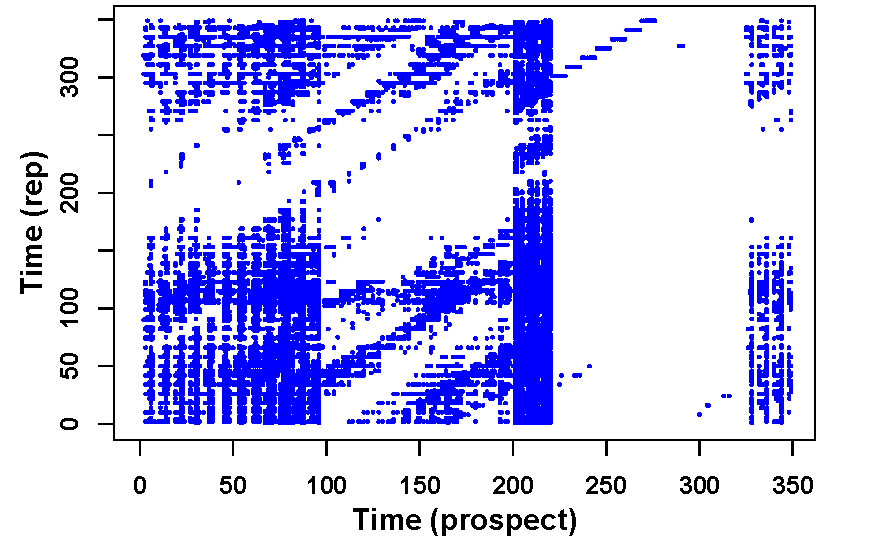
\includegraphics[width=\linewidth]{crqa_plot_115993376241473405}
	\caption[\acs{crqa} analysis of pitch in a sales call]
		{A recurrence plot generated for one of the analyzed conversations.
		The y-axis marks the conversation timeline, in time stamp, of the \ac{ae}, and the x-axis of the prospect.
		Each blue dot represents a co-visitation of a similar state.
		Blue dots forming an diagonal line indicate sustained recurrence between the two speakers (see description of NRLINE in \cref{subsec:output_values} for details).
		Note that the time stamps on the axes are not the slices, but the embedded call time.
		For example, the diagonal structures between time stamps 100 and 200 of the x-axis show such lasting recurrence.
		Diagonal lines above the \acl{los} (\acs{los}; the central diagonal line) indicate that the speaker on the y-axis leads the x-axis, and vice versa for lines below the \ac{los}.
		The blank area between time stamps 220 and 330 of the x-axis point to a portion of the call where the speakers were more distant from each other.}
	\label{fig:crqa_plot}
	\todo[inline]{make the plot square, to make it clearer that the times have the same length}
\end{figure}

\subsection{Recurrence detection}
\label{subsec:recurrence_detection}

\Ac{rqa} is a non-linear analysis method that quantifies the number and duration of recurrences withing a dynamical system presented by its state-space trajectory, which is typically the realization of a sampled time series.
It was introduced by \citet{Zbilut1992embeddings} and later extended by \citet{Webber2005recurrence, Marwan2002cross}.
A \emph{recurrence} (also, \emph{re-visitation}) is a time in which the trajectory returns to a state (or a similar-enough state, as explained below) it has visited before.
Recurrence can therefore be defined as the binary function

\begin{equation}
	\label{eq:recurrence}
	R_{i,j} =
	\begin{cases}
		1,	&	\text{if} \quad \lVert \vec{x}(i)-\vec{x}(j) \rVert_d \leq \varepsilon \\
		0,	&	\text{otherwise} \\
	\end{cases},
\end{equation}
%
where $i$ and $j$ are x-axis and y-axis coordinates in a recurrence plot (see \cref{fig:crqa_plot}), respectively, $d$ are the embedding dimensions, and $\varepsilon$ defines the threshold distance below which two cross-trajectory points are considered similar (see explanation about the \emph{radius} parameter in \cref{subsec:parameters_crqa}).
In a recurrence plot, the points $R_{i,j}$ are colored equal if their value is 1 or stay white otherwise.
\Ac{crqa} is an extension of \ac{rqa} analyzing recurrence quantification between two different time series rather than a single one time series with itself.
As such, \ac{crqa} is a quantification technique for non-linear dynamical systems that describes when and to what extent concurrences (or \emph{co-visitations}) can be found in a system consists of two time series.
These quantification techniques are based on \emph{recurrence plots} that for each moment $i$ in time show the times at which a phase space trajectory visits roughly the same area in the phase space as at time $i$.
Ultimately, a recurrence plot is a graph of $\vec{x}(i) \approx \vec{x}(j)$, showing $i$ on the x-axis and $j$ on the y-axis, where $\vec{x}$ is a phase space trajectory (see example in \cref{fig:crqa_plot}).
\todo[inline]{maybe take one of the RPs from the website and add the LoS (and other diagonals) to it to provide more detailed visualization?}
Each colored point in the plot represents a time where the time series were close to each other based on the definition in \cref{eq:recurrence}.
The main diagonal of the plot is called the \acf{los}.
A high number of recurrences along this line indicates synchrony between the time series.
However, diagonal recurrence lines can be formed above and below the \ac{los}.
Such diagonals, especially longer ones, represent delayed (lagged) synchrony between the time series and can be used as an assessment of similarity between the processes.
In the context of accommodation, these diagonals imply an accommodative change led by one of the interlocutors.
If the diagonal stretches above the \ac{los}, the speaker plotted on the x-axis leads the accommodation, and vice versa.
The closer the diagonal is from the \ac{los}, the quicker the process occurred, i.e., the led speaker aligned his behavior to the leading speaker after a shorter time.
Due to its ability to detect these similarities non-linearly, \ac{crqa} can be utilized to measure accommodation in the scope of entire conversations rather than taking only neighboring turns into account \citep[cf.][]{Levitan2013entrainment}.

\subsection{Parameter tuning}
\label{subsec:parameters_crqa}

\Ac{crqa} uses three parameters:

\begin{enumerate}
	\item \textbf{Delay} -- estimates the temporal shift required to make the two time series maximally aligned.
	It is measured by the same time unit as the time series, in the presented studies, a slice (see \cref{subsec:results_hhi}).
	
	\item \textbf{Embedding dimensions} -- are the number of dimensions into which the data points are embedded.
	These dimensions are delayed copies of the original time series $S(t)$ created by adding a lag $k$ to them.
	Typically, multiple lags are considered, which create the dimensions of embedding $S(t + nk)$.
	
	\item \textbf{Radius} -- determines the margin within which two data points are considered a recurrent instance.
	Distances between the data points are measured in the embedded space defined by embedding dimensions, using the same unit used for measuring the values of the time series.
\end{enumerate}
%
These parameters are a crucial key aspect in \ac{crqa} and how they are set is decisive for its outcome.
However, although some best-practice guidelines, like those suggested by \citet{Coco2014crqa-r}, exist, there is nevertheless no standard way for optimizing these parameters, especially due to the fact that they depend on the nature and characteristics of the data.
A method similar to the one presented by \citet{Marwan2007recurrence} was utilized in the analysis presented here.
The delay parameter was determined by finding the lag that minimizes the average mutual information between the two time series, which is determined by
%
% from https://www.frontiersin.org/articles/10.3389/fpsyg.2018.01679/full
\begin{equation}
	\label{eq:average_mutual_information}
	I\left( x(t), x(t + \tau) \right) = \sum_{i,j} p_{ij} (\tau) \log \left( \frac{p_{ij} \left( \tau \right)}{p_i p_j} \right).
\end{equation}
\eqname{Average mutual information (AMI)}
%
This provides a delay that is not too short to miss the different distributions, but also not too long to lose the dependency between the time series.
The lag with the \emph{lowest} average mutual information was selected, regardless of when the values started to level off.
Subsequently, the number of embedding dimensions was obtained using false nearest neighbors \citep{Kennel1992determining}.
This algorithm determines the minimum embedding dimension necessary to reconstruct the state space of a dynamical system with time delay embedding \citep{Abarbanel1993local}.
A neighborhood diameter equal to the standard deviation of the time series was used, and a limit of 20 embedding dimensions (which was never reached) was set.
\Cref{fig:ami,fig:false_nn} show examples of mutual information and false nearest neighbors optimizations.
%
\begin{figure}[H]
	\centering
	\begin{minipage}{.45\linewidth}
		\centering
		\includegraphics[width=\linewidth]{ami}
		\caption
		[Average mutual information of time series as function of lag]
		{The average mutual information of the time series values as a function of the lags considered.
			The x-axis shows the considered lags and the y-axis the mutual information index (AMI) in bits.}
		\label{fig:ami}
	\end{minipage}%
	\hfill
	\begin{minipage}{.45\linewidth}
		\centering
		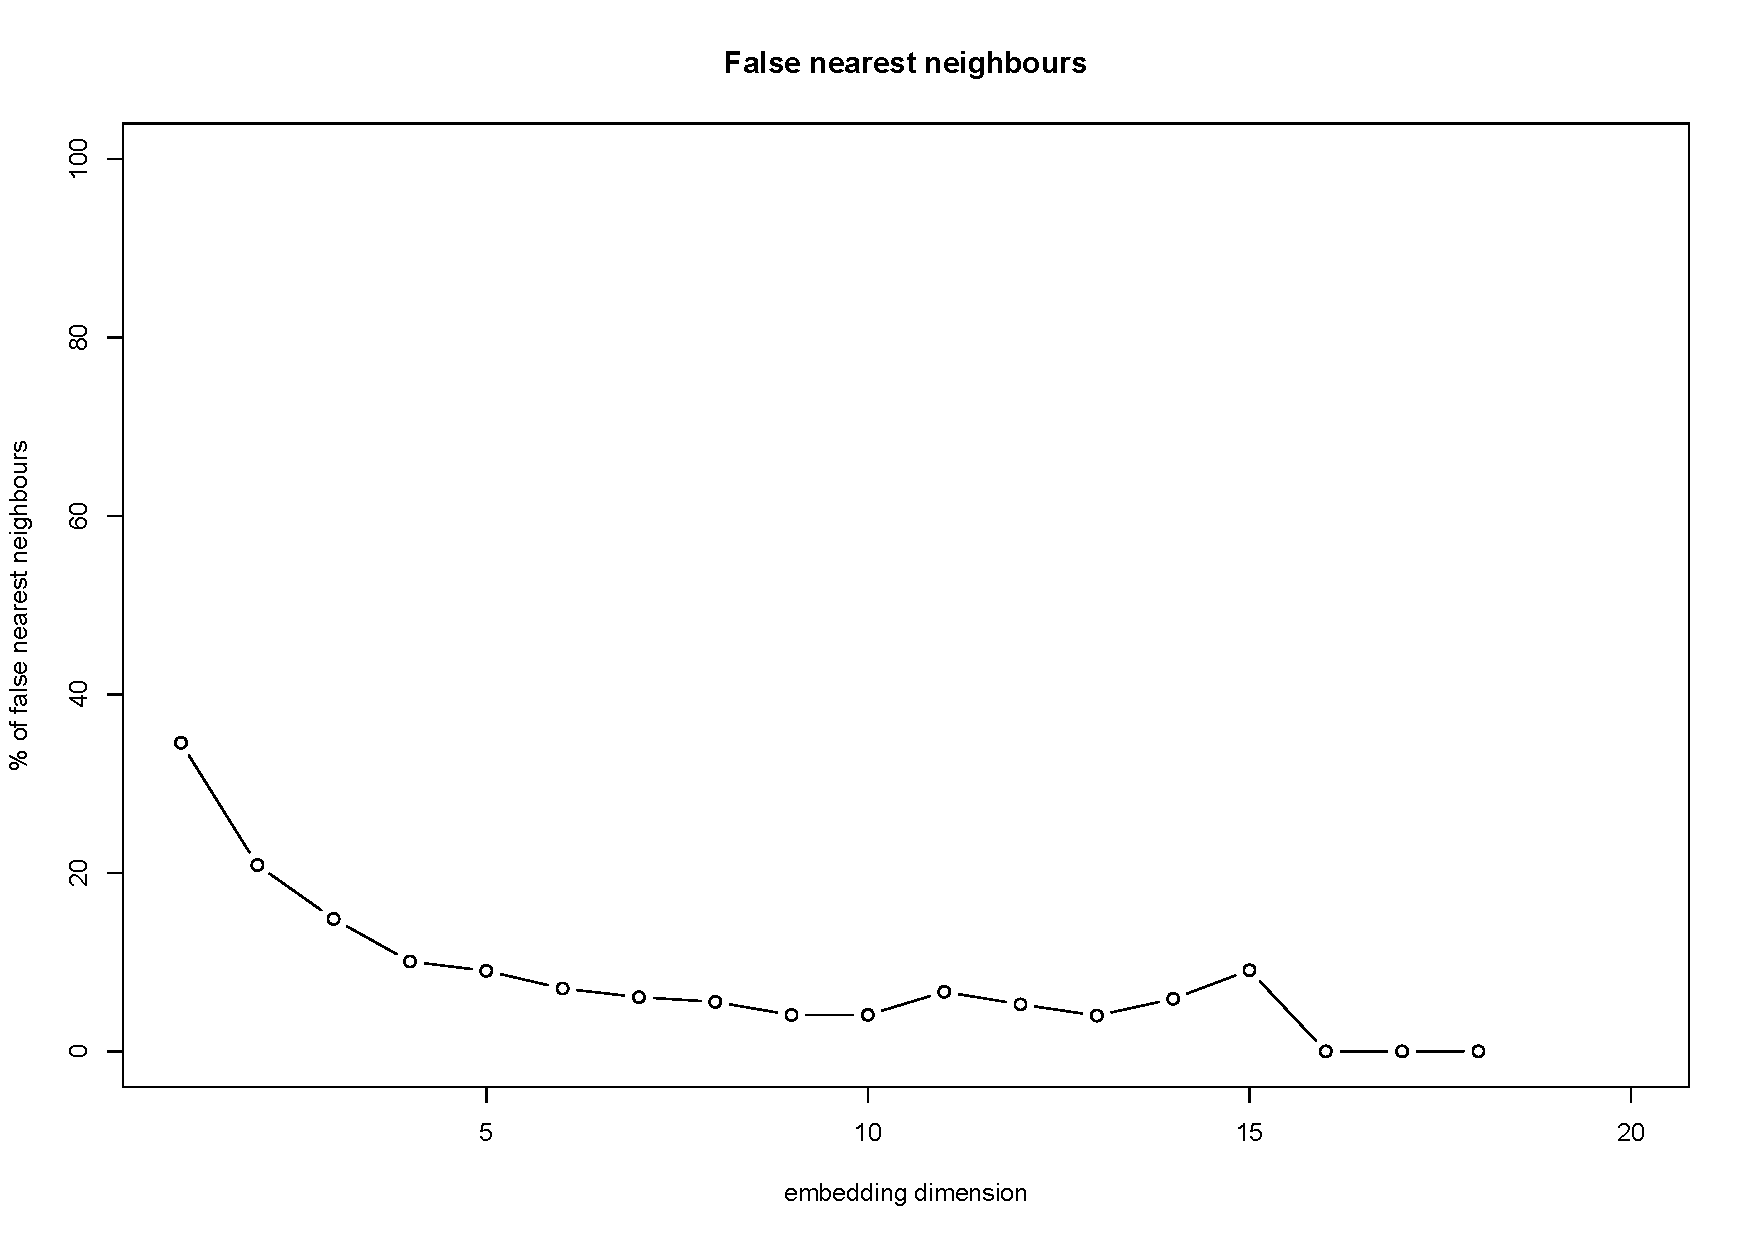
\includegraphics[width=\linewidth]{false_NN}
		\caption
		[Embedded dimensions optimization]
		{False nearest neighbours percentage as a function of the number of embedded dimensions.
			The x-axis show the considered numbers of embedded dimensions and the y-axis the percentage of false nearest neighbours.}
		\label{fig:false_nn}
	\end{minipage}	
\end{figure}
%
Following that, the radius was calculated in two steps (see \cref{alg:radius_opt}).
First, the goal \ac{rr} and a list of potential radii were initialized.
Here, the goal \ac{rr} was set to \SI{10}{\percent}, which is relatively high (e.g., compared to \SIrange{2}{5}{\percent} in \citet{Coco2014crqa-r}).
Setting the goal \ac{rr} to a higher value results in a stricter optimization that will reward closer recurrences.
The potential radii were generated by evenly spreading 20 candidates from 0 to the maximum value that occurs in the time series.
Then, each radius, along with the already optimized delay and embedding dimensions, was used to perform a \ac{crqa}.
A stricter policy was introduced in this step as well, as only lines longer than \SI{1}{\percent} of the time series' entire length were counted, as opposed to the typical setup that considers lines of any length.
With an average length of \SI{37.5}{minutes}, this means that lines longer than 11 time units, compared to the a typical setup with the minimal length of two time units (e.g., as done in \citet{Borrie2019syncing}).
This ensured that only long-term recurrences were taken into account, and shorter, possibly more random effects, were filtered out.
% note: calculated by multiplying 37.5 minutes * 60 to get seconds, then divide by 2 since each time unit (slice) was 2 seconds and again divide by 100 to get one percent of it.
Finally, the candidate radius that results in the smallest absolute distance from the goal \ac{rr} was chosen to perform the \ac{crqa}.
The radius optimization is described in \cref{alg:radius_opt}.
The optimization processes of all three parameters were done separately for each interaction.
%
\begin{algorithm}[t]
	\addtocounter{myequations}{1}
	\setcounter{myequations}{13}
	\caption{\acs{crqa} radius optimization}
	\label{alg:radius_opt}
	\algorithmcaption
		{\emph{The higher $n$ is (\cref{line:num_cand}), the higher the chance of a \ac{rr} close to the defined \emph{desired RR}.Also note that since \ac{rr} represents percentage of values in the recurrence plot, 100 is its highest possible value.
		Therefore, and since the radii in $R$ are traversed in increasing order, the search stops if this value is achieved(\cref{line:break_at_rr_100}).
		As explained in the text, in the presented studies $n = 20$ and $desiredRR = 10$ (see \citet{Coco2014crqa-r}).}}
	\DontPrintSemicolon
	\SetKwInOut{Input}{Inputs}
	\SetKwInOut{Output}{Output}
	
	\Input{\underline{$desiredRR$} -- the desired approximated \ac{rr} value\newline
		\underline{$optDelay$} -- the optimized delay\newline
		\underline{$optEmbedim$} -- the optimized embedded dimensions\newline
		\underline{$TS$} -- all values from both time series}
	\Output{radius producing \ac{rr} value closest to the defined desired \ac{rr}\newline}
	
	$n \gets$ number of radius candidates \label{line:num_cand}\;
	$R \gets \{r_i, \ldots, r_n\} : r_1 = 0, r_n = \max(TS)$\;
	$\forall r \in R : \lvert r_i - r_{i-1} \rvert = \lvert r_{i+1} - r_i \rvert$ \tcp*{evenly spread candidates}
	
	$candR \gets \varnothing$\;
	\ForEach{$r \in R$}{
		$currRR = crqa(ts_1, ts_2, optDelay, optEmbedim, \ldots\footnotemark).RR$ \tcp*{RR with candidate}
		$candR = candR \cup currRR$\;
		\uIf{$currRR = 100$}
		{\emph{break} \label{line:break_at_rr_100} \tcp*{\ac{rr} cannot be higher than 100}
		}
	}
	$optRadius = \displaystyle\argmin_{r \in R}(\lvert candR_r - desiredRR \rvert)$\;
\end{algorithm}
\eqname{Radius optimization algorithm for \acs{crqa}}
\footnotetext{As calculated by the \ac{crqa} package for R \citep{Coco2014crqa-r} with the additional arguments (unlisted in the algorithm itself) \emph{rescale=0, normalize=0, minvertline=length(ts1) / 100, mindiagline=length(ts1) / 100,} and \emph{tw=0}.}
%\todo{make sure algorithm block is on same page with its footnote and that the foot note is not cut into the next page}

\section{Dataset and feature extraction}
\label{sec:dataset_calls}

A collection of real-world calls with similar characteristics to those described in \cref{subsec:inside_sales} was used in this study.
These calls were all made by trained sales representatives and were aimed at high-stakes deals\footnote{In this case, around US\$100,000 each, as opposed to occasional mass calls to random people for selling small products where the losses are very small in comparison.
The reps in the calls collected here are aware of the deal scales and know that their performances are evaluated, pushing them to do their best in every single call.}.
To obtain a somewhat more homogeneous collection of conversations, calls of a single sales company (but multiple customer companies, see below) were selected.
Another constraint is that the collection comprises only calls from an early stage of the sales opportunity that is also the first encounter between the participating \ac{ae} and the prospect.
Therefore, behavior patterns that are not related to the history between the two interlocutors or the content of previous conversations between them can be identified.
Thus, these calls typically include a description by the prospects of their business' history, challenges and plans, followed by a demo by the sales person.
It is important to note that although every \ac{ae} prepares for such calls as part of the daily work, they are still spontaneous and in no way scripted.
%In some cases the prospect have already talked to an \ac{sdr} and/or communicated by email with the sales person.
%However, to the best of our knowledge, this is the first voice call with the prospect.
The calls in this collection were conducted using the Zoom platform, and were recorded automatically -- without any intervention from either side -- by Gong.io's system, which provides conversation intelligence services to said company.
Participants were notified of the recording, in compliance with all relevant laws and rights.
The calls were transcribed and diarized using an internal \ac{asr} system.

A single \ac{ae} and a single prospect participated in each call.
In total, 708 calls were used for analyses, each with a different customer company, with a total length of \SI{442}{hours} (mean 37.5 $\pm$15 minutes).
Furthermore, only calls longer than 15 minutes were selected, as shorter calls are often unsuccessful connection attempts or brief updates that are not representative for the desired conversation structure.
Call recording started immediately following the first greet from the prospect's side, and stopped when the meeting owner terminated it.
This eliminates segments during which one party is waiting for the other to join, and keeps only segments where both parties are present.
The 26 \acp{ae} (12 female) who participated in the calls formed 87 unique interlocutor pairs with different prospects.
Each prospect only ever spoke with one \ac{ae}.
The speakers on both sides were native speakers of American English.
For the purpose of this study, a call is defined as successful when a follow-up call under a more advanced stage is initiated or when an advancement in the opportunity is marked within one month.
These criteria follow common conventions of measuring call success\footnote{The benchmarks for successful deals are much more elaborate in practice and usually consider an entire selling process that comprises a series of calls.
However, many of those criteria are not relevant or cannot be enforced in the scope of this study.}.
This results in 51 calls (\SI{7.2}{\percent}) being defined as successful, which is within the industry standard ratio for this kind of calls.
Failed calls lasted on average 37 $\pm$15 minutes and successful calls 42 $\pm$16.5 minutes.
A two-sample Wilcoxon test \citep{Wilcoxon1945individual} between failed and successful call durations yielded a p-value of 0.04 with confidence level of \SI{95}{\percent}, confirming their differentiable distributions.
It goes without saying that the labels of both criteria are noisy, as sales opportunities might be lost because of parameters more related to the fit between the offered product and the prospect's needs, the available budget of the prospect, the presence of competitors, legal issues that tamper the deal etc.
To minimize such cases, calls done by personnel that are not sales people in the customer companies were filtered out.
%Following that, we hypothesized that successful sales calls would show more distinct speech patterns and vocal accommodation behaviors than unsuccessful calls.

As a preparation for the feature extraction and to increase temporal resolution, the audio signals were split into two-second slices (see motivation and further details in \cref{sec:analysis_hhci}).
Such fine-grained extraction makes the use of \ac{crqa} more elaborate, as it has more data points to consider (see \cref{sec:crqa}).
Splitting the turns also creates equal, consecutive, and more comparable time units for an interaction without introducing artificial boundaries by dividing it into a predefined number of parts.
The slicing was done per turn, so that a slice contains only the speech of a single speaker.
Any remainder of a turn got a slice of its own.
When a speaker is not speaking (e.g., during the turn of the other interlocutor), it is assumed that the last produced value is maintained until the speech is renewed and a new value can be measured.
This way, no discontinuities are created and the same number of data points is extracted for both speakers, which creates a better temporal representation of the conversation.
Feature extraction was done sequentially for all the conversations using Praat \citep{Boersma2001praat} scripts that extracted the \ac{f0} value from the middle of each slice and then post-processed the output to acquire cleaner measures.
Afterwards, the list of measures were turned into two equally long time series.
First, the values for each speaker were separated into two list.
Subsequently, missing values, e.g., due to non-speech slice, were replaced by the most recent valid value of their respective speaker, as motivated above.
Finally, if there were missing values at the beginning of a list, the first valid value of the that list was used, under the assumption that the first utterance represents the immediate time prior to it.
The resulting two lists had the same number of values representing the same timestamps along a single conversation, and were used for the \ac{crqa}.
Note that this process was performed individually for each conversation, regardless of whether one or more of the speakers participated in other conversations in the datatset.

\section{Analysis}
\label{sec:analysis_hhi}

Time series-based analysis methods like \ac{crqa} can be used in many ways.
The specific calculations used in this study are introduced below, followed by the results they yielded for the collection of sales calls and their interpretation.

\subsection{\Acs{crqa} output values}
\label{subsec:output_values}

Various measures can be computed based on a recurrence plot\footnote{See \citet{Marwan2007recurrence} and summary with additional measures in \url{http://www.recurrence-plot.tk/rqa.php}.}.
Some measurements deal with the \ac{los} and other diagonals across the plot while others consider vertical and horizontal lines.
Below are the definitions of some \ac{crqa} measurements used in this work.
For simplicity, it is assumed that the time series lengths are equal, so that $N_i=N_j=N$.

\begin{description}
	\item[\Acf{rr}] -- The percentage of recurrent points in the plot, i.e., the percentage of similar values between the two time series out of all the values.
	This corresponds to the correlation sum and defined as
	%
	\begin{equation}
		\label{eq:rr}
		RR = \frac{1}{N^2} \sum_{i=1}^{N_i} \sum_{j=1}^{N_j} R_{i,j}.
	\end{equation}
	\eqname{-- 4.4.5 CRQA-based measures: RR, DET, L, maxL, and ENTR}
	%
	This number generally corresponds to the overall colored area in the recurrence plot.
	The lengths of the time series ($N_i$ and $N_j$) are often -- but not necessarily -- equal
	
	\item[Determinism (DET)] -- The percentage of recurrences forming diagonal lines in the recurrence plot given a minimal length threshold $l_{\min}$.
	%
	\begin{equation}
		\label{eq:det}
		DET = \frac{\sum_{l=l_{\min}}^{N} l P(l)}{\sum_{l=1}^N l P(l)},
	\end{equation}
	%
	where $l$ is the length of a line and $P(l)$ is the histogram of the lengths $l$ of the diagonal lines.
	Note that $l=1$ refers to lines of length 1, i.e., a single recurrence point.	
	Similarly, $l=2$ are lines spanning over two time stamps (shortest length possible).
	This length is very forgiving in the case of accommodation, for such short lines can be formed arbitrarily and do not necessarily point to a meaningful accommodation process.
	Therefore, in the experiments presented here $l_{\min}$ was set to $\frac{N}{100}$, as in \cref{subsec:parameters_crqa}.
	
	Another measure, Laminarity (LAM), can be calculated the same way, but for the vertical lines in the plot.
	In that case, a $v_{\min}$ would be defined and $P(v)$ would provide the histogram of vertical line lengths.
	
	\item[Number of lines (NRLINE)] -- The total number of lines $N_l$ formed in the recurrence plot.
	In the context of accommodation, this is the number of accommodation \enquote{instances} between the two speakers lasting at least $l_{\min}$ time units.
	Also referred to as \emph{sustained recurrence} by \citet{Borrie2019syncing}, defined as the amount of alignment between conversational partners, where higher sustained recurrence values indicate higher amounts of sustained accommodation.
	As explained in the description of the measure \emph{DET}, only lines of length $\frac{N}{100}$ and longer were taken into account in the studies presented here to exclude \enquote{arbitrarily formed} diagonals.
	
	\item[Average length (L)] -- the average length of the diagonal lines, i.e., the average total accommodation time between the speakers.
	Higher value indicates longer average individual accommodation periods during the interaction.
	This is calculated by
	%
	\begin{equation}
		\label{eq:l}
		L = \frac{\sum_{l=l_{\min}}^N l P(l)}{\sum_{l=l_{\min}}^N P(l)}.
	\end{equation}
	%
	The average length of vertical lines, called trapping time (TT), is achieved in a similar way when using the same formula for the vertical line length and the histogram of vertical line lengths.
	
	\item[Maximal length (maxL)] -- The longest diagonal line in the plot, excluding the main diagonal.	
	This is the longest, uninterrupted time span over which accommodation between the speakers lasted.
	Higher value indicates a longer time span.
	The unit of this measure is the same as the axes of the plot (here, a representation of the conversation's turns).
	It is determined by
	%
	\begin{equation}
		\label{eq:maxl}
		L_{max} = \max_{l} (\{l_i; \ i=1, \ldots, N_l\}).
	\end{equation}
	%
	In a similar manner, the longest vertical line can be determined by traversing the vertical lines.
	
	\item[Entropy (ENTR)] -- The Shannon entropy of the probability distribution of the diagonal line lengths longer than the minimum length $l_{\min}$.
	Describes the variability of the amount of accommodation between the two speakers across the whole interaction.
	Higher value indicates more varied length of accommodation periods across the interaction.
	Shannon's entropy formula provides the value:
	%
	\begin{equation}
		\label{eq:entr}
		ENTR = -\sum_{l=l_{min}}^{N} p(l) \ln p(l),
	\end{equation}
	%
	where $p(l)$ is the probability of length $l$ from the lengths probability distribution.
	\item[Normalized entropy (rENTR)] -- The entropy value normalized by the number of lines formed in the recurrent plot.
	This measure helps understanding how the speakers vary across multiple calls with different characteristics.
\end{description}
%

\subsection{Results}
\label{subsec:results_hhi}

Since multiple variables are compared here, the Bonferroni correction \citep{Bonferroni1936teoria} was applied, so that the overall error rate across all variables is \num{0.05}.
Therefore, for a single comparison to be significant, it must be lower than $\alpha = 0.007$.
The non-parametric two-sample Wilcoxon test \citep{Wilcoxon1945individual} was used to determine the significance levels.
\cref{tab:crqa_results} shows a summary of means and p-values of the CRQA outputs for failed and successful calls.
The \ac{rr} mean value is about 10 in both groups, which proves to be a suitable goal for optimizing the parameters (see \cref{subsec:parameters_crqa}).
Significant differences between failed and successful calls were found for the values DET, NRLINE, and rENTR.
The first two, along with their higher means for the failed calls, indicate more time-synchronized convergence in the failed calls.
The latter is harder to interpret, especially due to the similar means for successful and failed calls.
It therefore seems that the behavior in both cases is evenly predicted -- but differently -- across calls.
One possible factor influencing these behaviors is related to the interlocutor leading the convergence effect, rather than the fact that it occurs at all.
The significant difference in the NRLINE measure stands in line with the findings in \citet{Borrie2019syncing}, supporting it as evidence for sustaining convergence in this study as well.
The same measures for measures were performed based on the leading speaker in each conversation (bottom part of the table), but no significant differences were found for this criterion.

\begin{table}[t]
	\caption{P-values of the two-sample Wilcoxon test comparing the \ac{crqa} output values based on call success/fail and leading speaker along with their respective mean values.
	See \cref{subsec:output_values} for details about each measure.
	Significant values based on the adjusted p-value threshold are set in bold.}
	\label{tab:crqa_results}
	\begin{tabularx}{\linewidth}{X
								 S
								 S[table-comparator=true, table-space-text-pre={$\ll$}]
								 S[table-comparator=true, table-space-text-pre={$\ll$}]
								 S
								 S
								 S
								 S}
		\toprule
						& {\thead{\acs{rr}}}	& {\thead{DET}} 		& {\thead{NRLINE}}		& {\thead{maxL}} 	& {\thead{L}} 	& {\thead{ENTR}} 	& {\thead{rENTR}} 	\\
		\midrule
		p (deal)		& 0.9					& \bfseries $\ll$0.001	& \bfseries $\ll$0.001	& 0.7 				& 0.07			& 0.1				& \bfseries 0.0058 	\\
		mean success	& 10.1					& 2.2					& 84.0					& 31.3 				& 17.8			& 1.4				& 0.8				\\
		mean fail		& 10.0					& 5.9					& 174.0					& 32.9 				& 15.3			& 1.5				& 0.8				\\
		\rule{0pt}{4ex}\\
		p (lead)		& 0.7					& 0.1					& 0.05					& 0.18				& 0.9			& 0.07				& 0.55				\\
		mean \acsp{ae}	& 10.0					& 6.1					& 186.7					& 35.2				& 15.2			& 1.5				& 0.8				\\
		mean prospects	& 10.1					& 5.4					& 154.4					& 31.2				& 15.7			& 1.4				& 0.8				\\
		\bottomrule	
	\end{tabularx}
\end{table}

To shed more light on the lead role in a conversation, \acl{cc} was used to determine which interlocutor leads the change in behavior.
As shown in \cref{fig:crqa_plot}, \ac{crqa} reports at which points in time the speakers were more inclined to be closer to each other.
As an extension, \acl{cc} finds the degree to which two time series are synchronized at different points in time.
For each such point, called \emph{lag}, the \acl{cc} function evaluates the correlation between the time series.
By iterating over a set of time points, the shift needed to make the time series maximally correlated can be found.
If this lag is positive, the first time series needs to be shifted forward to achieve maximal correlation, and vice versa.
In the context of convergence, \acl{cc} calculates the direction of the shift, which indicates the speaker leading the change.
The \acl{cc} function was not limited to a specific range of shifts, so that all possible lags were examined.
The lag associated with the maximal correlation, and only it, was used to determine the leader.
Since the calls in the collections used here have a typical structure, it is also interesting to see at which point of the conversation the maximal correlation occurs.
\cref{fig:barplot_conv_leaders} shows the time, in percent, in which the maximal correlation occurred for \acp{ae} and prospects in successful and failed calls.
The difference between the lag position distribution of reps and prospects is significant ($p = 0.0065$ with $\alpha = 0.05$).
However, the differences between successful and failed calls within the leading speakers are not significant.
It is also evident that when the reps were leading, they consistently did so at an early stage of the conversation, all the more so in successful calls, whereas the prospects' lead varied much more and generally happens at a much later time.
%
\begin{figure}[H]
	\centering
	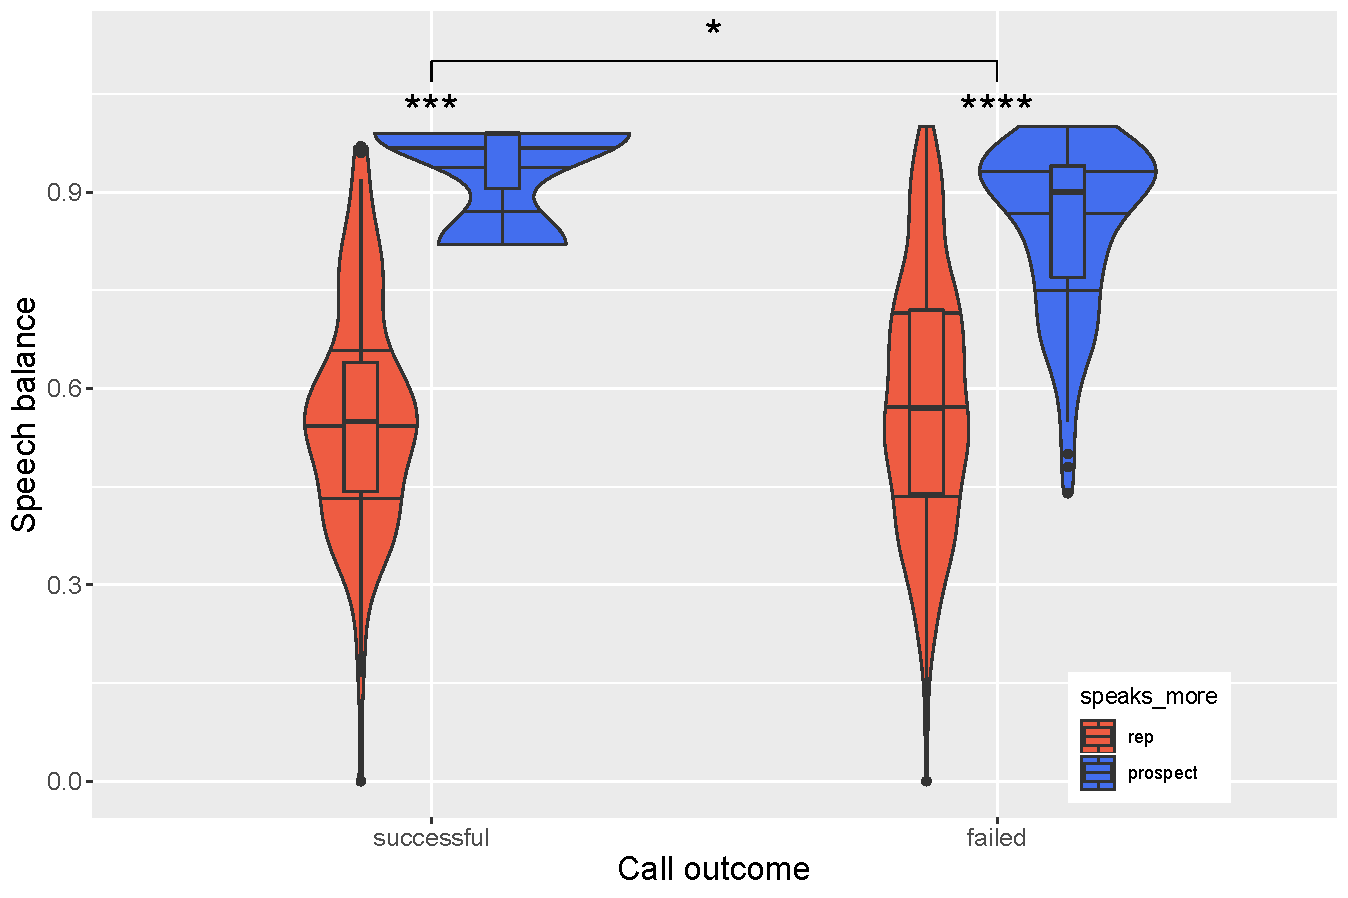
\includegraphics[width=\linewidth]{speech-balance_success_violin}
	\caption[Distribution of speech balance in successful and failed calls]
		{Comparison of speech balance distribution in successful and failed calls, sub-grouped by the speaker who spoke in total in individual calls (sales rep or prospect).
		The width of the shapes represent the probability density.
		The inner boxes show the central quartiles of the data with the median (excluding outliers) is marked by the thick horizontal line in it.
		The additional horizontal lines mark the \SI{25}{\percent}, \SI{50}{\percent}, and \SI{75}{\percent} quartiles of the data (including outliers).
		The asterisks stand the significance levels of the comparisons between the main groups (successful vs.\ failed) in the center and for the subgroups below it (* $p < 0.05$, *** $p < 0.001$, **** $p < 0.0001$)}.
	\label{fig:speech-balance_success_violin}
	\todo[inline]{could be easier to read if the inner boxplots had white fill and the quartile lines would be different color or a bit thicker}
\end{figure}
%
Another known conversational element in sales calls is the talk time each of the speakers get.
\Acp{ae} are trained to let the prospects speak as much as possible.
This is known to give them better feeling during the call, and also give the reps more information and opportunities to understand what their customers want to talk about.
All in all, this is good practice for keeping the \emph{speech balance}, i.e., the ratio between the total amounts of time in which speaker talked during the call.
Beside speech balance, the frequency and timing of speaker switching also sheds light on the dynamics of the speakers' vocal behaviors.
While each speaker should get sufficient amount of time to talk, it is also important to take and give the floor to the other interlocutor.
Long monologues can make the listener lose concentration or lack of expression, which damages the interaction.
Therefore, the \emph{interactivity} of the speakers is important as well.
While speech balance informs about the overall amount of time each speaker talked, interactivity complements this by informing how often a speaker gave the floor to the conversation partner.
Despite not being a concrete phonetic features, these two speech-related properties do fit into the overall notion of vocal accommodation nonetheless.
An analysis of these two additional conversation-level properties is performed here.
Speech balance was measured by
%
\begin{equation}
	\label{eq:speech_balance}
	speech\_balance = 
	1 - \left| \frac{\displaystyle \sum_{\forall S \in S_A} dur(S) - 
						\sum_{\forall S \in S_B} dur(S)}
					{\displaystyle \sum_{\forall S \in S_A \cup S_B} dur(S)}
		\right|,
\end{equation}
\eqname{Speech balance in conversation}
\noindent
%
where $S_A$ and $S_B$ are the slices in which speaker $A$ and $B$ speak, respectively and the function $dur$ returns the duration of a slice or set of slides.
The yielded value between 0 and 1 measures the percentage of balance in term of speech times, with 1 standing for \enquote{perfect balance}, i.e., equal talking times for both speakers.
As mentioned above, overall speech balance only reveals part of the whole picture.
Another part of it is the interactivity in the conversation, which is here defined as
%
%\begin{equation}
%	\label{eq:interactivity}
%	interactivity = 
%	,
%\end{equation}
%\eqname{Interactivity in conversation}
%\noindent
%
the percentage of slices, in which speaker change occurred after a consecutive slice sequence longer than some threshold (here, 1) without such change.
Sequences below this threshold can be generally ascribed to backchanneling, which does not indicate speaker change.
Interactivity and speech balance were measure for a superset of the dataset presented in \cref{sec:dataset_calls}.
\cref{fig:speech-balance_success_violin} shows the speech balance scores of successful and failed calls.
On the one hand, it is clear that lower the balance the more likely it is that reps had more floor time.
The recommendation to avoid imbalance is reflected by the significant difference between balance distribution in successful and failed calls.
On the other hand, prospects are only likely to talk more when the balance score is high, even more so in successful conversations.
This evident by the highly significant differences in both sub-groups.
No significant influences of interactivity on call outcome were found, and only a weak correlation between speech balance and interactivity was found. % r=0.2
%
\begin{figure}[H]
	\centering
	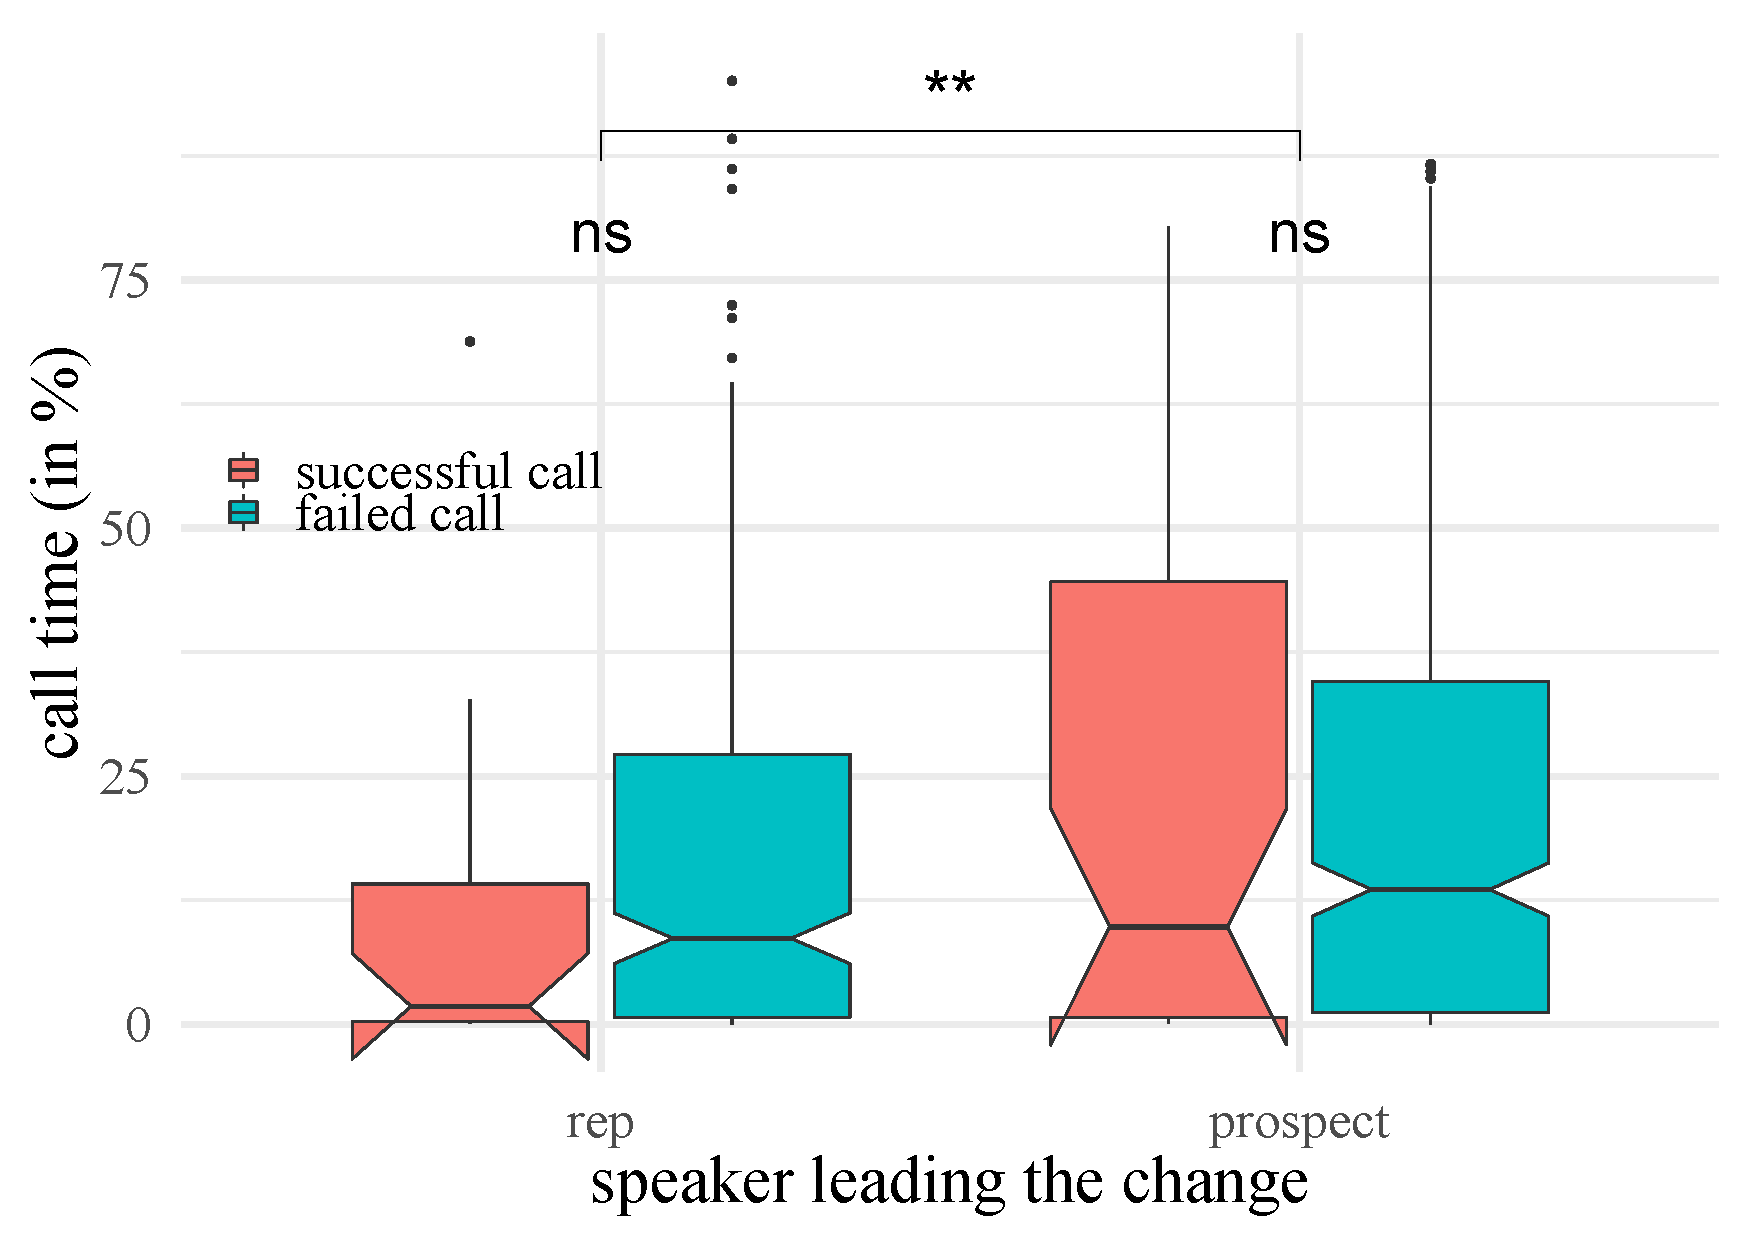
\includegraphics[width=\linewidth]{boxplot_ccf}
	\caption[Comparison between sales reps' and prospects' maximal \acl{cc} point in conversation for successful and failed calls.]
		{Comparison between the time of the call in which the maximal \acl{cc} occurs.
		The x-axis groups the calls based on the speaker, and the fill color further separates the calls to successful and failed ones.
		The y-axis points to the time in the call, in which the maximal correlation was detected.
		The horizontal lines within the boxes represent the median,
		the notches stand for the \SI{95}{\percent} confident level of the median, the area inside the boxes include the \acf{iqr} of values, the vertical lines outside the boxes show the value within the third quartile + 1.5$\protect\cdot$\ac{iqr}, and the isolated dots are the outliers.
		The significance level based on a Wilcoxon test comparing the two groups and their subgroups is given above the boxes.}
	\label{fig:barplot_conv_leaders}
	%	\todo[inline]{use logarithmic y-scale?}
\end{figure}
%

\section{Discussion}
\label{sec:discussion_hhi}

The results of the study show two sides of \ac{crqa} with respect to call success and role detection.
On the one hand, successful and failed calls could be distinguished by three of the \ac{crqa} output values.
Although based on \ac{hhi} studies it might be hypothesized that recurrence is more likely to occur in successful calls, the means of two of the three values suggest the opposite.
Yet, this stands in line with some studies from sales research that show more \enquote{desperate} behavior from the rep side when a call seems to fail.
This includes unconsciously showing assimilation towards the prospect, and over-emphasizing the deal's \ac{roi}, with the hope that it will convince the prospect to buy \citep{Orlob2018roi}.
However, these often achieve the opposite effect and are therefore discouraged in the sales industry.
Another possible explanation is that reps give up their own lead in the call (see below) when a call is on the verge of failing, and instead let the prospects lead, either as a natural tendency or to give them a better feeling.
This, too, is a known effect in sales business.
On the other hand, utilizing \acl{cc} lags (i.e., how the recurrence needs to shift for the speakers to be maximally aligned) was useful for differentiating between the leader in the calls.
When \acp{ae} lead, they tend to do so at an earlier stage than prospects, especially in successful calls.
This, together with the \ac{crqa} results shown in \cref{subsec:results_hhi}, suggests that \acp{ae} do not necessarily always lead the conversation, but know when to exploit this technique, consciously or not, to improve their stance in calls.

Though beyond the scope of this work, three further investigation directions on this topic are suggested here:
First, deepening the aspect of the relationship between the \acp{ae} and the prospects by examining the mutual changes not only within single calls, but over the course of an entire deal spanning over several meetings.
This could shed light on long-term changes and connect changes to the success of the deal.
Secondly, distinguishing between different \acp{ae} to find behaviors of sub-groups or identifying star reps.
For example, sales persons with higher ratings might be revealed to better exploit accommodation and trigger different behavior on the prospect side to increase their chance of closing a deal.
Lastly, different methods could be applied to predict the success of a call.
Specifically, machine learning methods that are good at capturing serial changes, such as recurrent neural networks, can be used to train such prediction models.
All of these direction can also be combined with more features to uncover more consistent accommodation patterns.

% Conclusion
%We have presented a study that examines phonetic accommodation in real-world sales calls.
%The focus was on mutual proximity of \acl{f0} between sales persons and prospects to find both how close they are to each other in general across the call, and how quickly changes in proximity occur and by whom they are initiated.
%This was done by \acf{crqa} and \aclp{cc}, which together provide various measures regarding recurrence between the speakers and who leads the other in terms of \acl{f0} changes.
%A corpus of 708 calls was used for the analyses, which makes it possible to find more global, consistent effects that are not influenced by the design of a specific experimental setting.
%The results show significant differences in some of the values between successful and failed calls, and significant differences between the leading behavior of sales persons and prospects.
%These findings encourage further investigations, like looking for other predictors of successful calls and examining the influence of additional features and factors on the success of calls.

\chapter{Shadowing Experiments with Natural and Synthetic Voices}
\label{chap:shadowing_experiment_with_natural_and_synthetic_voices}

\lettrine{A} series of experiments is described in this chapter.
Some of them were designed to determine human behavior in \acl{hhi} and \ac{hci} as a mean of modeling interactions, and others examined the change in reactions of subjects to different adaptation strategies of implemented system as a subjective evaluation method.

\pagebreak

\section{Shadowing paradigm}
\label{sec:shadowing_paradigm}

\todo[inline]{general explanation what experimental setting is (with references)}
\todo[inline]{why is it good for accommodation experiments.}
\todo[inline]{explain different between online and offline shadowing (better terms?)}
\todo[inline]{briefly say that both experiments here are offline shadowing}

\section{Alignment in novel and familiar sung music}
\label{sec:alignment_in_novel_and_familiar_sung_music}

\todo[inline]{motivation to do this experiment. relation and differences to linguistic accommodation}

\subsection{Experimental design}
\label{subsec:design_music}

\subsubsection{Target features}
\label{subsubsec:target_features_music}

\subsubsection{Stimuli and participants}
\label{subsubsection:stimuli_participants_music}

\subsubsection{Procedure}
\label{subsubsec:procedure_music}

\subsection{Analyses and results}
\label{subsec:results_music}

\section{Convergence to natural and synthetic stimuli}
\label{sec:convergence_to_natural_and_synthetic_stimuli}

something\ldots

As always in accommodation studies, \SI{100}{\percent} would mean complete convergence to every stimulus, which cannot be reasonably expected.

\subsection{Experimental design}
\label{subsec:design_HCIConv}

Phonetic convergence is often examined in the scope of shadowing experiments, in which the participants are asked to repeat utterances spoken by an interlocutor \citep[e.g.,][]{Pardo2017phonetic, Dias2016visibilivty, Walker2015repeat, Shockley2004imitation}.
This is typically done with single words as targets.
The experiment showcasing our system in \cref{sec:showcase} uses whole sentences as stimuli, in which the target features are embedded, making it a semi-conversational \ac{hci} setting.

\subsubsection{Target features}
\label{subsec:target_features_HCIConv}

\todo{little intro}

Although these feature may pass as light dialectical markers \citep{Mitterer2013regional}, they do not carry any difference in meaning, and are generally ascribed to personal preference of speaking style.

\begin{enumerate}    
	\item \textbf{\textipa{[\c{c}]} vs.\ \textipa{[k]} at a word-final $\langle$-\textit{ig}$\rangle$} syllable
	
	These variations of the phoneme \textipa{[\c{c}]} are both common native speakers of German.
	Using one variation or the other does not change the meaning of the word, or any other property of it.
	Although it can be generally said that \textipa{[\c{c}]} is more used in the south and \textipa{[k]} in the north of Germany, they do not mark a specific dialect or socio-economic status.
	This \enquote{neutrality} makes this feature a good candidate, since change in pronunciation should not occur due to the liking of one dialect or the other, or as an attempt to match a certain social status.
	It is noteworthy that the \textipa{[\c{c}]} variation is considered to be more standard, but still, both of the variations are accepted and people typically do not even notice which variation they and their interlocutors are using.
	In this experiment, we treat this feature as bi-categorical in nature.
	The very few instances of other fricatives (such as \textipa{[S]} and \textipa{[J]}) were counted as \textipa{[\c{c}]} as well, making the distinction practically between fricative and plosive realization.
	Here are two examples of sentences with this features that were used as material for the experiment's stimuli (for the full list of stimulus materials, see \autoref{app:shadow_experiment_stimul}):
	
	\begin{enumerate}[label=\arabic{enumi}\alph*), ref=\arabic{enumi}\alph*.)]
		\item 
		\begin{tabulary}{\linewidth}{LLL}
			Der & köni\textbf{\underline{g}} & hält eine Rede.\\
			\textit{The} & \textit{king} & \textit{spoke}.\\
		\end{tabulary}
		\item
		\begin{tabulary}{\linewidth}{LLLLL}
			Ich & bin & süchti\textbf{\underline{g}} & nach & Schokolade.\\
			\textit{I} & \textit{am} & \textit{addicted} & \textit{to} & \textit{chocolate}.\\
		\end{tabulary}
	\end{enumerate}
	
	\item \textbf{\textipa{[e:]} vs.\ \textipa{[E:]} realization of the mid-word grapheme \enquote{ä}}
	
	These two phonemes represent the two extremes of this feature's realization.
	However, vowel quality, as opposed to the \textipa{[\c{c}]} vs.\ \textipa{[k]} feature, it is not categorical (fricative vs.\ plosive), but rather gradual.
	That means that the actual realization can be anywhere between these two extremes.
	Despite the gradual nature of vowel quality, native speakers still perceive this feature as categorical (either \textipa{[e]} or \textipa{[E]}, cf.\ \citet{Kuhl2004early, Kuhl1991human}).
	\review{are these references relevant? is this really magnet effect?}
	In this experiment, we treat this feature as categorical in the first phase (see \cref{subsubsec:procedure_hci}), but measure it as gradual for analysis purposes (see \cref{subsec:results_hci}).
	This allows the detection of non-categorical changes over time, which are important for characterizing the convergence process.
	The \textipa{[E]} variation is in general more typical for the southern federal states of Germany, while \textipa{[e]} is more common in the north.
	As in the case of the \textipa{[\c{c}]} vs.\ \textipa{[k]} feature, the use of one realization or the other (or any in-between them) does not make any difference in meaning.
	Here are two examples of sentences with this features that were used as material for the experiment's stimuli (for the full list of stimulus materials, see \autoref{app:shadow_experiment_stimul}):
	
	\begin{enumerate}[label=\arabic{enumi}\alph*), ref=\arabic{enumi}\alph*.)]
		\item 
		\begin{tabulary}{\linewidth}{LLLLL}
			War & das & Ger\textbf{\underline{ä}}t & sehr & teuer?\\
			\textit{was} & \textit{the} & \textit{device} & \textit{very} & \textit{expensive}?\\
		\end{tabulary}
		\item
		\begin{tabulary}{\linewidth}{LLLLLL}
			Ich & mag & die & Qualit\textbf{\underline{ä}}t & deiner & Tasche.\\
			\textit{I} & \textit{like} & \textit{the} & \textit{quality} & \textit{of your} & \textit{bag}.\\
		\end{tabulary}
	\end{enumerate}
	
	\item \textbf{\textipa{[@n]} vs.\ \textipa{[\s{n}]} at a word final $\langle$-\textit{en}$\rangle$ syllable}
	Unlike the two previous features, this feature does not, typically, show variation in -- all the more so in spontaneous speech, which is more relevant in the context of \acp{sds}.
	While the \textipa{[@n]} variation may occur when one wants to emphasize the word/syllable or when speaking more clearly, e.g., with children or when in a noisy environment, the \textipa{[\s{n}]} variation is by a large margin the more dominant one.
	It is rare to hear consistent production of a \textipa{[@n]} in an ending-syllable $\langle$-en$\rangle$.
	This is true across-dialects and regions, and it is ascribed to the phonological rule \textit{schwa elision} that occurs in the German language, as follows \citep[adapted from][pp.~142--143]{Benware1986phonetics}:
	%
	\begin{equation}
		\text{\textipa{@n}}\longrightarrow \varnothing \text{\textipa{\s{n}}} \diagup
		%	\left[\text{$-$son}\right] \ \_\_ \ \{\text{\#}, \left[\text{+const}\right]\} .
		\text{+consonantal} \ \_\_ \ \ \text{\#} .
		\label{eq:elision_rule}
	\end{equation}
	\eqname{Phonological process: Schwa elision in German}
	%	
	Here are two examples of sentences with this features that were used as material for the experiment's stimuli (for the full list of stimulus materials, see \autoref{app:shadow_experiment_stimul}):
	
	\begin{enumerate}[label=\arabic{enumi}\alph*), ref=\arabic{enumi}\alph*.)]
		\item 
		\begin{tabulary}{\linewidth}{LLLLL}
			Wir & besuch\textbf{\underline{en}} & euch & bald & wieder.\\
			\textit{We} & \textit{will visit} & \textit{you} & \textit{soon} & \textit{again}.\\
		\end{tabulary}
		\item
		\begin{tabulary}{\linewidth}{LLLLLL}
			Sind & die & Küch\textbf{\underline{en}} & immer & so & groß?\\
			\textit{Are} & \textit{the} & \textit{kitchens} & \textit{always} & \textit{so} & \textit{big}?\\
		\end{tabulary}
	\end{enumerate}
\end{enumerate}



\todo{say that there were some filler whose purpose was to check the they can pronounce these sounds at all}

\todo{also talk a bit the differences between the nature of the features, i.e. categorical vs. gradual, vs. mostly perceptual + gradual length + realization of length of next nasal}

\subsubsection{Stimuli and participants}
\label{subsubsection:stimuli_participant_hci}

\todo{what was the age of the participants? how many males and females?}
\todo{mention how many stimuli in total, how many fillers, how many for each feature etc.}

\subsubsection{Procedure}
\label{subsubsec:procedure_hci}

\todo{probably better to put the more graphical version, but the existing one file size is too big}
\begin{figure}[!t]
	\centering
	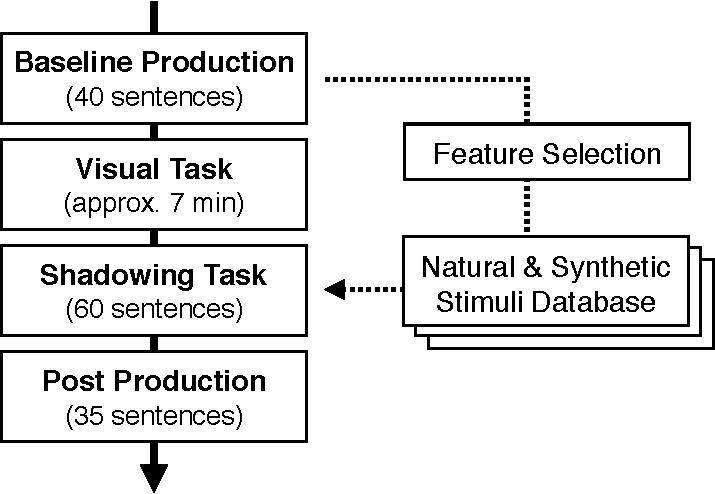
\includegraphics[width=\linewidth]{flow_experiment}
	\caption[\acs{hci} convergence experiment workflow]{Workflow of the experiment, showing its four phases. The stimuli presented in the shadowing task are selected based on feature realization in the baseline production.}
	\label{fig:HCIConvFlow}
\end{figure}

The experiment was carried out in a sound-proof booth located inside a recording studio.
Seeing that the experiment dealt with the way people change their way of speaking based on speech of others, conversation with participants was generally kept as minimal as possible.
It goes without saying, however, that it was not realistic to try and control for any kind of conversation the participants might have had during the day prior to the experiment.

%%%%%%%%%%%%
% text taken originally from System chapter

The experiment consists of three phases: \emph{baseline} production, \emph{shadowing} task, and \emph{post} production (see \cref{fig:HCIConvFlow}).
In the \emph{baseline} phase, the participants were asked to read out the stimuli from a monitor.
The participant's most frequent variant in this phase is configured into the system.
Then, in the \emph{shadowing} task, the participants produced the stimuli sequentially, each after listening to another voice (either natural or synthetic, both male and female) producing the opposite category of the relevant target feature.
Based on the production in this phase, the participant's tendency, pace, and degree of convergence were analyzed.
Finally, in the \emph{post} phase, the participant once again read out the stimuli from a screen.
The purpose of this phase was to examine whether any convergence remained in effect even in the absence of non-preferred input.
%%%%%%%%%%%%%%%%%%%

In the first phase of the experiment, the base natural production of the participants was observed.
No instructions whatsoever were given regarding how they should speak.
An overview of the workflow in presented in~\autoref{fig:HCIConvFlow}.
The participants were to read 40 sentences from a monitor.
\review{explain fillers etc.}
The sentences were all in grammatical German and relatively short (5-7 words), with some being declarative and some interrogative.
No signal was introduced to tell the participants to start reading (aside from the sentence to appear on the monitor after a blank \enquote{pause} screen), and the average pausing time between uttering two sentences was
\todo{insert time}
milliseconds.
Utterances of sentences containing a target feature were examined on-the-fly, and the way they were produced by the participant was marked.

The second phase was a short pause, about seven minutes long.
Its purpose was to let the mental representation of the production to fade, so that the base production will not influence as much on the productions in the following parts.
To boost this process, the participants played a game with strong visual aspects and with non-verbal sounds only.
Conversing with the participant was avoided as much possible as possible in order to prevent from other verbal input to influence their mental representations.
The participants' performance in the game was not recorded and did not influence the next parts in any way.

The third phase

The fourth and final phase

A Java-based program with \ac{gui} was developed exclusively for this experiment.
Its functionality was tailored for the setup and the phases described above.
This includes test sentences for setting up output volumes (participant's headset, experimenters' speaker, etc.), auto shuffling the stimuli into a balanced list, convenient way of choosing the correct stimuli from the database (correct set plus considering the participant's pronunciation preferences), logging the times and stimulus order, playing and replaying stimuli, and more.
\todo[inline]{screenshot of the program or at least a more detailed description (semi-randomization etc.)}

\subsection{Analyses and results}
\label{subsec:results_hci}

\begin{figure}[!t]
	\centering
	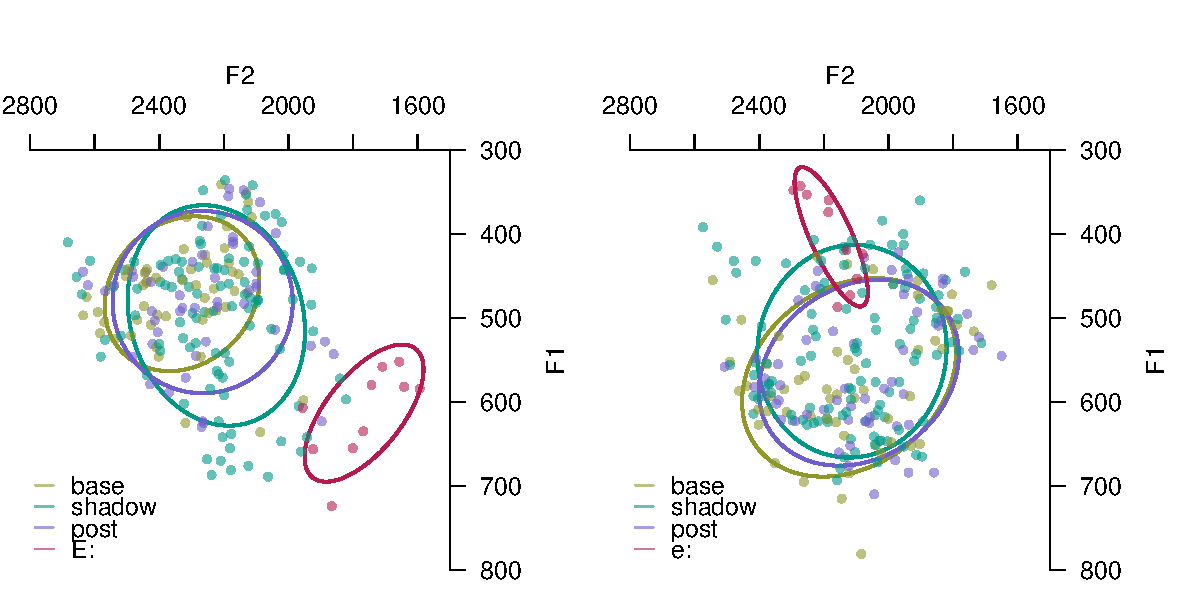
\includegraphics[width=\textwidth]{formant-plot}
	\caption[short caption]{long caption}
	\label{fig:HCIConvFormants}
\end{figure}

\fixme{how to put schwa and ic-ik next to each other?}

\begin{figure}[!t]
	\centering
	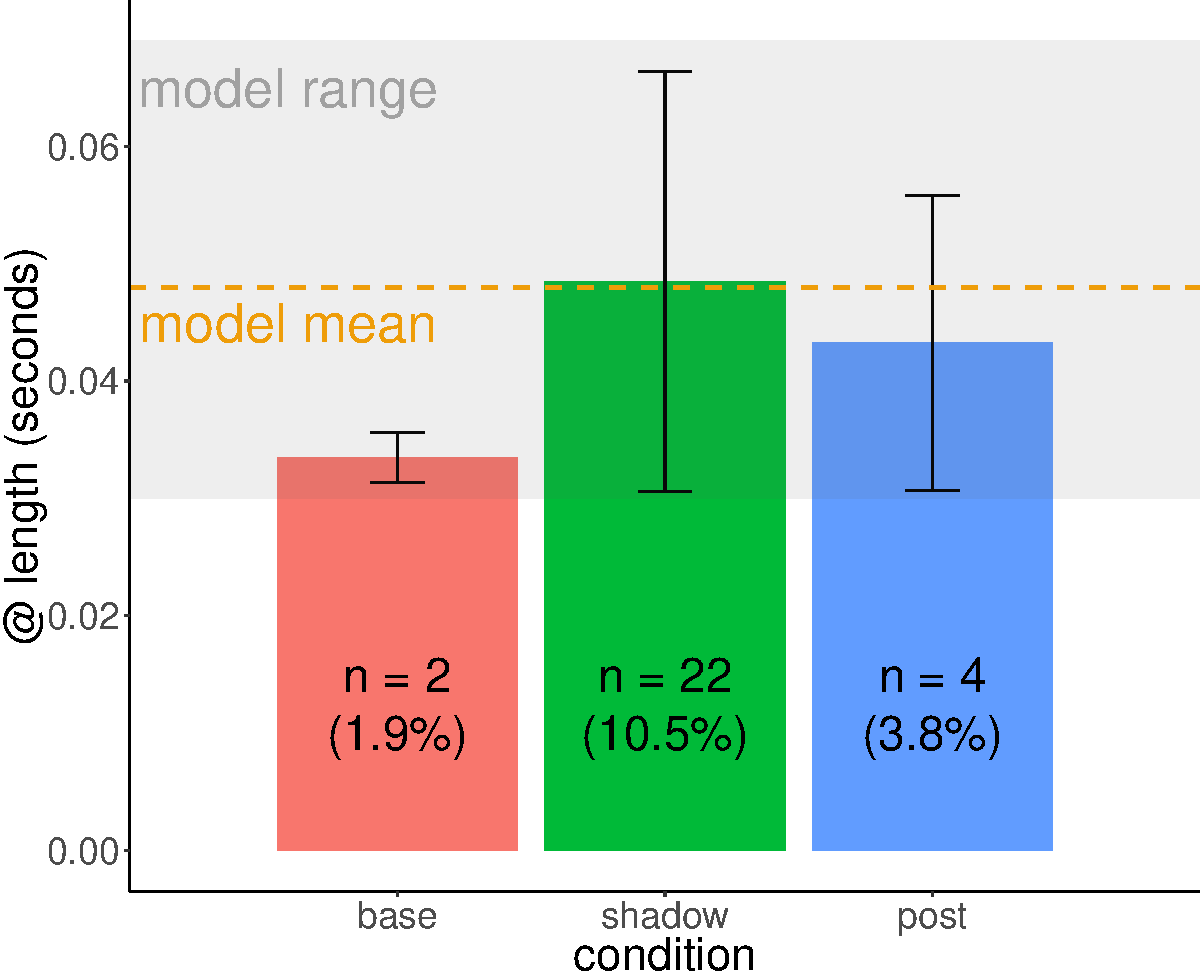
\includegraphics[width=0.5\textwidth]{schwa-plot}
	\caption[short caption]{long caption}
	\label{fig:HCIConvSchwaPlot}
\end{figure}

\begin{figure}[!t]
	\centering
	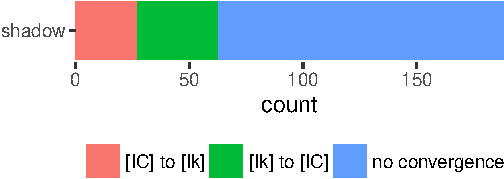
\includegraphics[width=0.5\textwidth]{ich_ik-plot}
	\caption[short caption]{long caption2}
	\label{fig:HCIConvIcIkPlot}
\end{figure}

\subsection{Generation of the synthetic stimuli}
\label{subsec:generation_stimuli_hci}

After finding some convergence effect to the natural stimuli, the next step is to test whether the same convergence effect is present also occurs when presenting synthetic stimuli to the participants.
For that, synthetic (i.e.\ computer generated) stimuli need to be created.
There are multiple methods to synthesize speech:
formant synthesis \citep[e.g.][]{Burkhardt2000verification}, unit selection \citep{Hunt1996unit,Black2003unit}), diphone synthesis \citep{Dutoit1996mbrola}, and probabilistic (e.g., using \acp{hmm} as described in \citet{Zen2005overview} and in \citet{Zen2009statistical}), to name some.

Seeing that the experiment in question examines convergence in specific segment-level phonetic features, it is preferable to fix other speech characteristics like intonation and stress, in order to prevent from those to influence the perception of the sentences by the listeners.
To achieve that, the f$_0$ contours and segment durations of the natural stimuli were imposed on the synthetic stimuli.
These values were extracted from the annotations of the natural stimuli (see \citet{Gessinger2016PundP}):
The segment durations were directly taken from the annotations, and the f$_0$ contours were acquired by first interpolating the contour of the natural stimuli, and then record the f$_0$ value at the beginning and at the middle of each segment.
These two values per segment were used in the synthesis.
It goes without saying, however, that the generated contours were not \emph{completely} identical to those of the corresponding natural stimuli, but no substantial differences in overall sentence intonation or stress were introduced.

\section{Conclusion}
\label{sec:conclusion_shadowing}
\chapter{Accommodation in Multiparty Interaction with An Agent}
\label{chap:speech_variations_in_hhci}

\lettrine{M}{ore} dynamic vocal behaviors can be established in interaction with more than two speakers.
This is not only due to additional possible connections between interlocutors, but also because of additional factors that might influence them as well, like the order of speech or the role of each speaker.
A \acl{hhci} study is presented in this chapter, where the effects of different aspects and conditions on vocal accommodation are investigated.

\pagebreak

\section{Speech variations in human-human-computer interaction}
\label{sec:accommodation_in_multiparty_interaction_with_an_agent}

Nowadays, we are witnessing in our everyday lives an ever-growing presence of devices with spoken interaction capabilities, like \acp{pa}, speech-activated cars, hands-free medical assistants, and \acp{its}, to name a few.
As argued in \cref{subsec:personal_assistants}, the use of \acp{pa} is rapidly increasing, as more every-day tasks can be achieved using them.
The question arises, therefore, whether different speech patterns and characteristics emerge in such \ac{hci} than in \ac{hhi}; and if yes, which.
One way of measuring such changes is in terms of linguistic similarity between the interlocutors.
It has been demonstrated that humans may change their speech behavior when interacting with computer-based systems.
In various \ac{hci} experiments, participants have been shown to speak differently to computers in general, and also change their speech during the interaction (see \citet{Branigan2010linguistic}, for examples).
The vast majority of experimental work done in the field of vocal accommodation deals with the smallest possible social interactions, namely dyadic conversations.
Those can be dyads of two human speakers, forming \ac{hhi}, or a human and some computer-based agent, which results in \ac{hci}.
Vocal accommodation in these types of interactions is explored in \cref{chap:shadowing_experiment_with_natural_and_synthetic_voices,chap:conv_analysis}.
However, social interactions may also be multiparty, consisting of three or more participants.
this is true for both \ac{hhi} and \ac{hci}, but also for interactions with mixed human and computer-based interlocutors.
The last can occur in various situations, like a person consulting a \ac{va} regarding availability in a weekly schedule while setting an appointment with a colleague or two friends ordering tickets from a voice-activated machine.
Such mixed multiparty interactions already take place in our every-day lives.
Their popularity -- and sometimes necessity -- increase alongside the rise in use of \ac{c-ai} devices, such as \acp{va}, voice-activated cars, social robots, etc.
It is important, therefore, to investigate whether convergence, divergence, and other effects (see \cref{subsec:variation_types}) can be found not only in \aclp{hci}, but in \acp{hhci} as well.
Various \ac{hci} experiments have shown that participants speak differently to computers in general, and also change their speech behavior during the interaction, e.g., by \citet{Branigan2010linguistic} and \citet{Levitan2016implementing}.
And yet, no previous work in the field performed a direct comparison between different human-directed and computer-directed speech couplings within a multiparty interaction.
If any direct comparison is done in empirical \ac{hci} experiments, it typically focuses on computer-based interlocutors only and emphasizes the influences of different system configurations on the interaction \citep[e.g.,][]{Levitan2016implementing}.
Moreover, only the influence of the system's speech output on the user speech is examined, but not the influence of other human interlocutors.

Empirical work on multiparty \ac{hci} includes experiment where participants interact with different types of agents, like social robots \citep[as in][]{Foster2012two,Ibrahim2019fundamental} and human avatars in immersive virtual worlds \citep[e.g.,][]{Traum2002embodied}.
Even in dyadic form, spoken interactions are a hard task for computers.
All the more so, when more than one other interlocutors are involved.
Measuring accommodation becomes more complex with multiple interlocutors involved, as discussed in \citet{Rahimi2019acoustic}.
There are many technical challenges on the way to realistic, real-time interactions with computers, including -- but not limited to -- center-of-attention detection, active speaker detection, turn taking, understanding private and shared knowledge, and of course correct speech production and understanding.
Interactions with machines are challenging for humans, too, since the former do not behave and react the same way (and usually speed) as humans.
An example of such a social activity, which is easy for humans to learn but still far from being accomplished by social robots, along with ways to cope with it, are described in \citet{Jonel2018Farmi}.
The type and severity of those problems depend also on the type of computer-based agent.
For instance, embodied agents at least have some basic way to convey non-verbal information, whereas voice-only systems like \acp{va} do not.
On the one hand, this gives a wider range of expressions to embodied systems, but requires more communication channels to implement on the other hand.
See \cref{sec:types_of_sdss} for more information about the different types of computer-based agents.

This chapter presents a study that examines interaction-level vocal accommodation in a \acf{hhci} scenario, focusing on distributional and temporal analyses of three phonetic features (see \cref{sec:analysis_hhci})
In this paradigm, two human speakers interact with an agent to complete tasks with a common goal.
More details about the dataset and the tasks are in \cref{sec:vacc}.
Investigating such a scenario contributes to the understanding of both the role of an agent in interactions with multiple humans and the role of one human interlocutor on the other.
These two aspects are examined in the two \emph{components} of the study:
The \emph{addressee} component focuses on the differences between the participants' addressed interlocutor within a conversation \citep[][see]{Raveh2019ESSV}, and the \emph{crowd} component spotlights the influence of an additional human interlocutor on the participants' speech toward the agent \citep[see][]{Raveh2019InterspeechAlexa}.
The question tackled by the second component is whether and to what extent speaking to a second human interlocutor in addition to Alexa influences the accommodation in interaction with a \ac{va}.
More generally, it investigates whether users speak differently towards a computer-based system when another human participates in the interactions.
The performed analyses in \cref{sec:analysis_hhci} are based on the participants' \emph{speech directions}, i.e., \acf{hds} and \acf{dds}, as illustrated in \cref{fig:condition_comparison_addressee,fig:condition_comparison_crowd}.
The comparisons were made based on the tasks performed by participants using the \ac{va} in both components, alternately interacting with the \ac{va} alone or with a confederate.
\todo{need more motivation for the two components?}

\section[The voice assistant conversation corpus]{Dataset} % \acl{vacc} doesn't work for some reason
\label{sec:vacc}

The \acf{vacc}\footnote{\url{http://www.iikt.ovgu.de/iesk/en/Research+Groups/MDS/Research/VACC-p-4624.html}}, introduced in \citet{Siegert2018VACC}, was utilized to examine these differences.
This corpus is suitable as it comprises both \acp{hci} and \acp{hhci} (\emph{solo} and \emph{confederate} conditions) with a 2\textsuperscript{nd} generation Amazon Echo Dot device with the skills and a female voice of the \acf{va} Alexa.
Other studies, like \citet{Shriberg2013addressee,vanTurnhout2005identifying}, used similar corpora to study automatic addressee detection.
The present work does not set detection and classification as a goal, but rather aims to provide insights and measures that might be useful for such tasks.
In the \ac{vacc}, the confederate was only present in the room only during tasks in the confederate condition and always sat at the same location.
To simulate the spatial situation of a multi-party interaction with a \ac{va}, the participant and the male confederate sat in similar distance from the device that was situated on a table, roughly forming an equilateral triangle shape in a living room-like environment (see Figure 2 in \citet{Siegert2018VACC}).
The participant had led the interactions, and the confederate never initiated the interaction.
Moreover, the confederate interacted only with the participant and never with Alexa.

%Two high-quality neckband microphones (Sennheiser HSP 2-EW-3) were used to capture the voices of the participant and the confederate speaker.
%Additionally a high-quality shotgun microphone (Sennheiser ME 66) captured the overall acoustics and the output of Amazon's Alexa.

In both conditions, two interactions took place, one for each task of the performed tasks:
The participant's goal in the calendar task is to find available time slots for several appointments with the confederate.
The participant's pre-defined calendar is stored on the device and is accessible only by inquiring Alexa.
In the solo condition, the participants got written information about the confederate's availability, whereas, in the confederate condition, the confederate could be asked directly about it, resulting in \acp{hhi} along side the \acp{hci}.
\cref{fig:conditions_comparison} illustrates the relations in each condition.
The goal of the quiz task is to answer trivia questions, e.g., \enquote{When was Albert Einstein born?}
Since Alexa was not always able to immediately provide a full answer to all the questions, the required information could be gathered incrementally in multiple steps.
Here, the participant solved the quiz alone in the solo condition or teamed up with the confederate so the two could discuss the question-asking strategy in the confederate conditions.
The quiz task is generally less formal than the calendar task.
%
\begin{figure}[t]
	\centering
	\subfigure[Solo condition]
	{\raisebox{1.85cm}{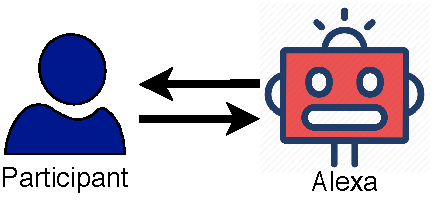
\includegraphics[width=0.45\textwidth]{condition_solo}}
	\label{fig:condition_solo}}
	\hfill
	\subfigure[Confederate condition]
	{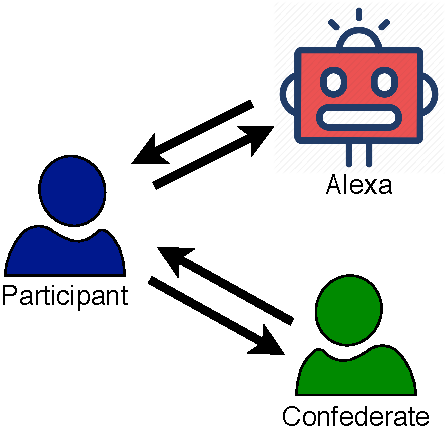
\includegraphics[width=0.45\textwidth]{condition_confederate}
	\label{fig:condition_confederate}}
	\caption[Solo and confederate conditions in \acs{hhci} setting]
		{Illustration of solo and confederate conditions.
		A black arrow represents direction of speech from speaker to addressee.
		Note that the confederate (in green) never talks or addressed by Alexa, but only the participant (blue).}
	\label{fig:conditions_comparison}
\end{figure}
%
The calendar task is designed so that the way to its solution is relatively straightforward:
Query the device for possible times till a match is found.
This requires interacting mostly -- if not only -- with the computer-based interlocutor.
Indeed, this task typically elicited interactions, in which the participant interacted with the confederate or the device in discretely separate turn blocks in the confederate conditions.
\ac{dds} blocks were, unsurprisingly, longer, as the confederate was only needed when additional information about the task was required.
The way to solve the quiz task is more flexible, because the strategy as to which questions to ask Alexa can be determined by the participant, including the amount and frequency of the confederate's intervention in the confederate conditions.
Indeed, this led to a more dynamic alteration between \ac{hds} and \ac{dds} in this task.

The dataset contains recordings of 27 (14 female) German native speakers in the age range of 20 to 32 years (mean 24 $\pm$3.3).
Each participant performed the quiz and calendar tasks in both solo and confederate conditions, for a total of 108 interactions (2 tasks $\times$ 2 conditions $\times$ 27 participants).
%An interaction was finished either by completing the task or by stopping it prematurely in case no further progress could be made, to avoid participant frustration.
%The latter, however, happened only a few times.
These interactions consist of approximately \num{13500} utterances, which were manually transcribed and annotated (speaker, speech times, addressee, etc.) and stretch over total recording time of \SI{17}{\hour} \SI{7}{\minute} (\SI{31}{\minute} average interaction length).
The permutations of the tasks, conditions, and their order were balanced.

%\begin{figure}[!h]
%	\begin{center}
%		\fbox{\parbox{6cm}{
%		This is a figure with a caption.}}
%		\includegraphics[scale=0.5]{image1.eps} 
%		\includegraphics[width=0.75\linewidth]{figures/IMG_4798.jpg}
%		\caption{A snapshot of the data collection setup. The confederate speaker (left side) and the participant (right side) are sitting around a table, where the voice assistant (Amazon Alexa Echo Dot) is located.}
%		\label{fig:wohnzimmer}
%	\end{center}
%\end{figure}


%The recordings were stored in WAV format with \SI{44.1}{\kilo\hertz} sample rate and 16 bit resolution.
%The recordings were manually separated into utterances, which were additionally annotated with its speaker, context, and textual transcription.
%The speaker of each utterance could be the participant, Alexa, or the confederate.
%The context marked the type of interaction of the utterance, which include \ac{hds}, \ac{dds}, cross-talk, off-talk, laughter, and more.
%To deal with clearer data, only \ac{hds} and \ac{dds} contexts were used for analysis in this paper.
%The transcription was obtained using the Google Cloud Speech API automatic speech recognition service.
%\cref{tab:dataset_charact} summarizes the dataset characteristics.

%\begin{table}[t]
%	% \captionsetup{format=plain,justification=raggedleft,width=.4\textwidth,hangindent=0pt,skip=500pt}
%	\centering
%	\caption{\ac{vacc} dataset characteristics}
%	\label{tab:dataset_charact}
%	\begin{tabular}{L{3cm}L{3cm}}
%		\toprule
%	     Participants 				& 27														\\
%	     Sex 						& Male 13 / Female 14 										\\
%	     Total Recorded Data 		& \SI{17}{\hour} \SI{7}{\minute}							\\
%	     Experiment Duration 		& Mean: 31 min 												\\
%		  Age (years)				& Mean 24 (Std: 3.32)										\\	% Min: 20; Max: 32  \\
%	     Language 					& German													\\
%	     Annotation 				& Transcription, Addressee, Laughter, Cross-Talk, Off-Talk	\\ 
%	     Supplementary self-reports & Evaluation of interaction, AttrakDiff, Speaking style, Experiences in interacting with voice assistants\\
%		\bottomrule
%	\end{tabular}
%\end{table}

\begin{figure}[t]
	\centering
	\subfigure[\acs{hds} in confederate condition]
	{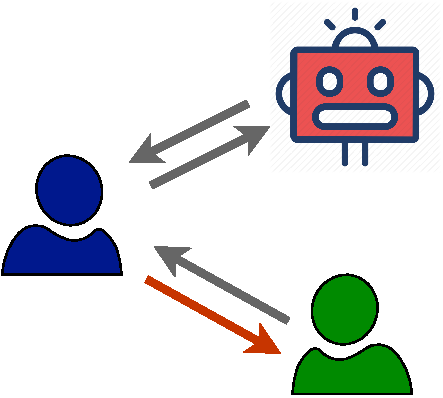
\includegraphics[width=0.45\textwidth]{condition_confederate_marked_hhi}
	\label{fig:condition_confederate_marked_hhi}}
	\hfill
	\subfigure[\acs{dds} in confederate condition]
	{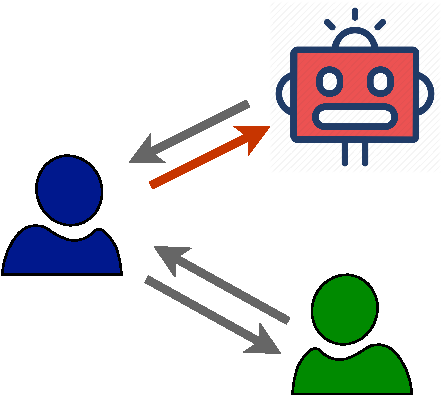
\includegraphics[width=0.45\textwidth]{condition_confederate_marked_hci}
	\label{fig:condition_confederate_marked_hci}}
	\caption[\acs{hds} and \acs{dds} compared in confederate condition]
		{Illustration of the compared speech directions in the \emph{addressee component}.
		The orange arrows mark the compared speech directions.}
	\label{fig:condition_comparison_addressee}
\end{figure}

\begin{figure}[t]
	\centering
	\subfigure[\acs{dds} in solo condition]
	{\raisebox{1.6cm}{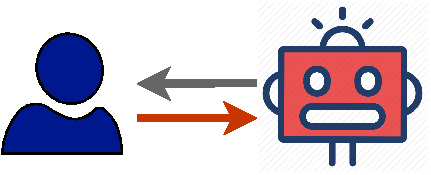
\includegraphics[width=0.45\textwidth]{condition_solo_marked}}
	\label{fig:condition_solo_marked}}
	\hfill
	\subfigure[\acs{dds} in confederate condition]
	{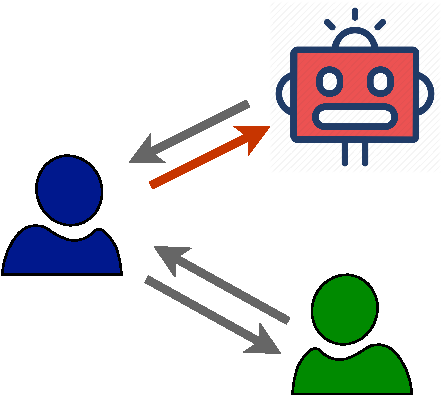
\includegraphics[width=0.45\textwidth]{condition_confederate_marked_hci}
	\label{fig:condition_confederate_marked_hci_crowd}}
	\caption[\acs{dds} compared in solo and confederate conditions]
		{Illustration of the compared speech directions in the \emph{crowd component}.
		The orange arrows mark the compared speech directions.}
	\label{fig:condition_comparison_crowd}
\end{figure}

\subsection{Annotations}
\label{subsec:annotations_hhci}

Each utterance in an interaction was annotated with its speaker, context, and textual transcription.
The speaker of each utterance could be the participant, Alexa, or the confederate.
Cross-talk was rare, as the participants typically waited till the confederate or Alexa finished talking (exception occurred when they tried to interrupt Alexa mid-utterance when the response was undoubtedly wrong or irrelevant due to recognition error).
The context marks the utterance's interaction type, like \ac{hds}, \ac{dds}, cross-talk, off-talk, laughter, and more.
To deal with clearer data, only \ac{hds} and \ac{dds} contexts were used for analysis, which, together, constitute over \SI{90}{\percent} of the overall recording time.
The transcriptions were obtained using the Google Cloud Speech API automatic speech recognition service and were subsequently manually verified and corrected.
Utterances' start and end times were directly derived from the timestamps of these annotations.

\section{Analysis}
\label{sec:analysis_hhci}

A suitable subset of the entire dataset (see \cref{sec:vacc}) was used for the analysis of each factor (see \cref{sec:accommodation_in_multiparty_interaction_with_an_agent}).
Only the 54 interactions from the confederate conditions were used for the addressee component, as the alternation between \ac{hds} and \ac{dds} within an interaction was examined.
For the crowd component, all 108 interactions were taken, because the comparison required executions of the tasks performed in both solo and confederate conditions.
Interactions of all 27 participants were included in both subsets.
Despite the different sizes of the subsets, the number of comparisons was the same for both factors, since the addressee component used two both speech directions of the participants in each interaction (54 $\times$ 2 = 108) and the crowd component used only one speech direction but from both conditions (54 $\times$ 1 + 54 $\times$ 1 = 108).
These subsets were analyzed based on the audio signals and the annotations described in \cref{subsec:annotations_hhci}.
The speaker annotations were used to determine to which of the three speakers the measured values should be ascribed.
The text transcriptions were only used to verify the correct audio segments were analyzed.
Comparisons were made between the speech directions in the same interaction, i.e., within a single task.

To increase temporal resolution, the audio signals were cut into two-seconds \emph{slices}.
A single slice always contained audio from a turn of a single speaker.
Any remainder shorter than \si{2} seconds got a slice of its own.
For example, a turn of \SI{5.2}{\second} in length was sliced into three slices of \SI{2}{\second}, \SI{2}{\second}, and \SI{1.2}{\second}.
This way, each slice contained speech of a single interlocutor.
Splitting the turn also creates equal, consecutive, and more comparable time units for an interaction without introducing artificial boundaries by dividing it into a pre-defined number of parts \citep[as in][]{Silber-Varod2018prosodic}.
This is especially important for the temporal analysis (\cref{subsec:temporal_analysis}).
Slice lengths of 0.5, 1, 5, and 10 seconds were experimented with as well.
However, those were found too short to capture changes in \ac{ar}, which is dependent on the size of this window, or two long to for a comparable and uniform temporal resolution.
Two seconds was found to be a good compromise based on these criteria.
%
The following phonetic features were targeted: 
%
\begin{description}%[wide=0pt, leftmargin=0.5\parindent, nosep]
	\item[\Acf{f0}] -- mean pitch measured within a slice with hop size of \SI{100}{\milli\second} and a defined range between \SIlist{60;350}{\hertz}.
	\citet{Gregory1993Voice} found that this feature is used to produce social similitude and cohesiveness in dyadic interviews.
	\citet{Babel2012role} found convergence effects in this feature in an auditory naming task and \citet{Bulatov2009effect} found similar effects in a shadowing task.
	
	\item[Intensity] -- mean intensity measured within a slice with hop size of \SI{100}{\milli\second}.
	This feature showed significant entrainment effect in game scenarios in \ac{hhi} experiments described in \citet{Levitan2011measuring}.
	Accommodation effects in this feature were also found by \citet{Natale1975convergence}.
	
	\item[\Acf{ar}] -- the ratio of the number of syllables to phonation time within a slice, as described in \citet{DeJong2009arcitulcationrate}.
	\citet{Schweitzer2013convergence} examined this feature in the context of phonetic convergence, but no effect was found on turn-level and interaction-level analyses.
\end{description}
%
All features were measured individually in each slice automatically using Praat \citep{Boersma2001praat} scripts.

\section{Results}
\label{sec:results_hhci}

Two analyses were carried out: distributional and temporal.
The first looks at global differences on the interaction level of the participant's and the computer-based interlocutor's productions between solo and confederate conditions.
It also examines whether the order in which the tasks were performed had any influence on the changes (see \cref{tab:signif_conditions,fig:signif_cases_ordered}).
The second examines time-based, continuous changes in the proximity between the participant's and the device's productions with an emphasis on the context factor (\ac{dds} or \ac{hds}), and provides additional insights for the factors \emph{sex}, \emph{task}, and \emph{order} (\cref{fig:condition_convergence_comparison,fig:alluvial}).

\subsection{Distributional analysis}
\label{subsec:distributional_analysis}

As a first measure of speech characteristics, the means, medians, and \aclp{sd} of the selected features in the participants' speech in each of the interactions were calculated in \ac{hds} and \ac{dds}.
The absolute values reflected in the means and medians can shed light on the overall range of values used with each of the two interlocutors, due to, for example, their gender (Alexa was always set with a female voice and the confederate was always male) or assumed comprehension capabilities of humans and computers.
The variability in the \aclp{sd} reflects of each interlocutor may indicate a different production behavior.
\todo[inline]{is it meaningful to have a table with these lists/values?}
Each target feature was measured and listed chronologically throughout the interaction.
These lists were divided into four distributions based on speaker and context:
the participant talking to the confederate, the participant talking to Alexa, the confederate talking to the participant, and Alexa talking to the participant (cf.\ four speech directions in \cref{fig:condition_confederate}).
The contrast between \ac{hds} and \ac{dds} is observable within the participant's speech only, which was active in both contexts.
The significance level of the difference between these two distributions was measured using a two-sample t-test with $\alpha=0.05$.

\Cref{fig:hds_dds_dist_signif,fig:hds_dds_dist_nonsignif} show examples of the distributions of a participant's \ac{f0} in \ac{hds} and \ac{dds} contexts.
Since Alexa always used a female voice and the confederate was always male, there is a natural gap between their \ac{f0}.
This gap leaves room for convergence to occur, i.e., change in the participants' production -- either temporarily or fixedly -- in the direction one of the other interlocutors.
As \cref{tab:results_hhci_addressee} shows, in \SI{74}{\percent} of the cases out of the 54 analyzed interactions the difference of the participant's \ac{f0} between \ac{hds} and \ac{dds} was significant.
Out of those, in \SI{85}{\percent} of the cases \ac{dds}'s distribution mass contained higher values than \ac{hds}'s, which indicates assimilation towards Alexa.
%
\begin{figure}[t]
	\centering
	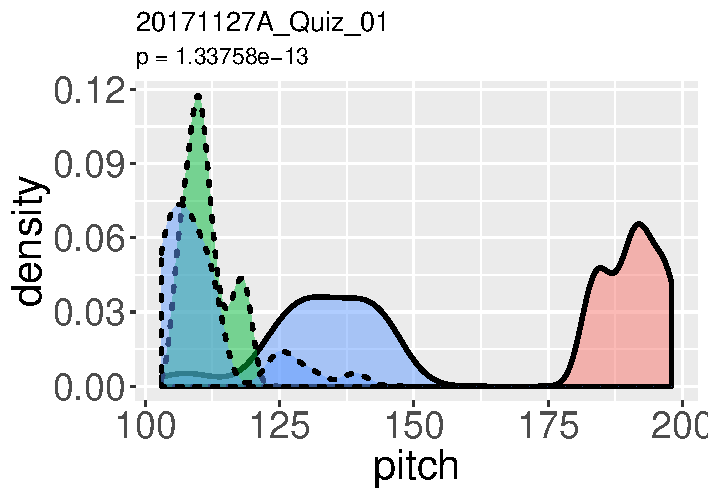
\includegraphics[width=\linewidth]{20171127A_Quiz_01_pitch_dist}
	\caption[An interaction with significant \acs{hds} and \acs{dds} \acs{f0} distributions difference]
		{An example of \ac{hds} and \ac{dds} distributions with a \emph{significant} difference (p-value~$\ll$~0.0001 with $\alpha=0.05$) extracted from the \ac{f0} measures in the quiz task of participant 20171127A.
		The colors represent distributions of Alexa (red), the confederate (green), and the participant (blue).
		The line style differentiates between \ac{hds} context (dashed line) and \ac{dds} context (solid line).}
	\label{fig:hds_dds_dist_signif}
	\todo[inline]{change p value notation in figure to <<}
\end{figure}
%
\begin{figure}
	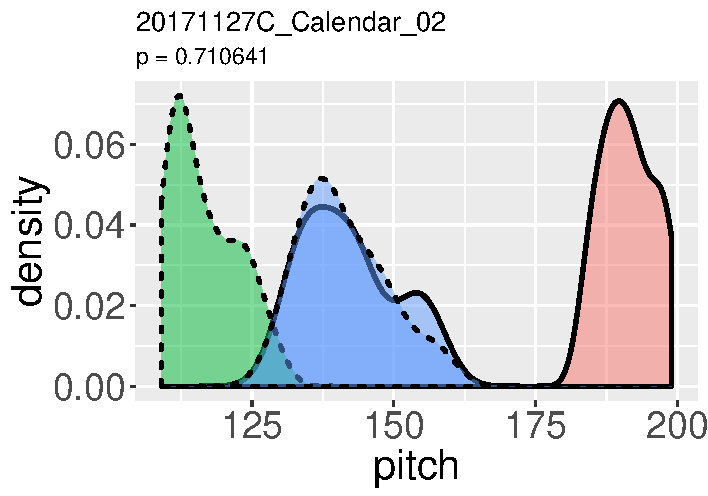
\includegraphics[width=\linewidth]{20171127C_Calendar_02_pitch_dist}
	\caption[An interaction with insignificant \acs{hds} and \acs{dds} \acs{f0} distributions difference]
		{An example of \ac{hds} and \ac{dds} distributions with a \emph{insignificant} difference (p-value~=~0.71 with $\alpha=0.05$) extracted from the \ac{f0} measures of participant 20171127C in the calendar task.
		The colors represent distributions of Alexa (red), the confederate (green), and the participant (blue).
		The line style differentiates between \ac{hds} context (dashed line) and \ac{dds} context (solid line).}
	\label{fig:hds_dds_dist_nonsignif}
	\todo[inline]{change p value notation in figure to <<}
\end{figure}
%
%\cref{fig:hds_dds_violin_intensity_comparison} shows examples of the distributions of the participant's intensity in \ac{hds} and \ac{dds} contexts.
Unlike in the case of \ac{f0}, absolute measured values of intensity may not be as meaningful due to the device's and the confederate's location relative to the participant's microphone, was used for the different analyses
This means that the absolute values of the participant's intensity in \ac{hds} and \ac{dds} can be compared directly, but only indirectly with Alexa's and the confederate's.
Therefore, the differences in \cref{fig:hds_dds_dist_signif,fig:hds_dds_dist_nonsignif} can be compared within a context, but the values should only be compared within the participant's speech (in blue).
In \SI{89}{\percent} of the cases the difference of the participant's intensity between \ac{hds} and \ac{dds} was significant.
Generally speaking, participants tended to speak to Alexa with a louder voice than to the confederate.
%
\begin{figure}[t]
	\centering
	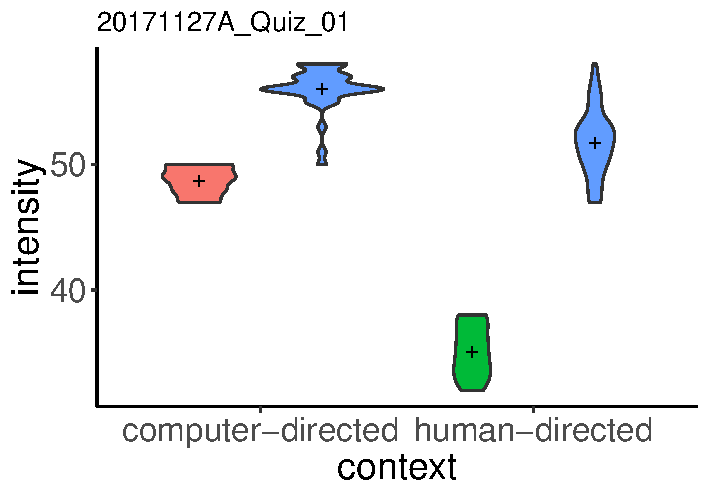
\includegraphics[width=\linewidth]{20171127A_Quiz_01_intensity_violin}
	\caption[An interaction with significant \acs{hds} and \acs{dds} intensity distributions difference]
		{An example of \ac{hds} and \ac{dds} distributions with a \emph{significant} difference (p-value~$\ll$~0.0001, $\alpha=0.05$) extracted from the intensity measures of participant 20171127A in the quiz task.
		A non-significant example is presented in \cref{fig:hds_dds_violin_nonsignif}.
		The colors represent distributions of Alexa (red), the confederate (green), and the participant (blue).
		The width of the box represents the frequency of the values and the \enquote*{+} sign marks their respective means.}
	\label{fig:hds_dds_violin_signif}
	\todo[inline]{legend and units for y-axis}
	\todo[inline]{explain in text that comparison is only relative between two blue components}
\end{figure}
%
\begin{figure}
	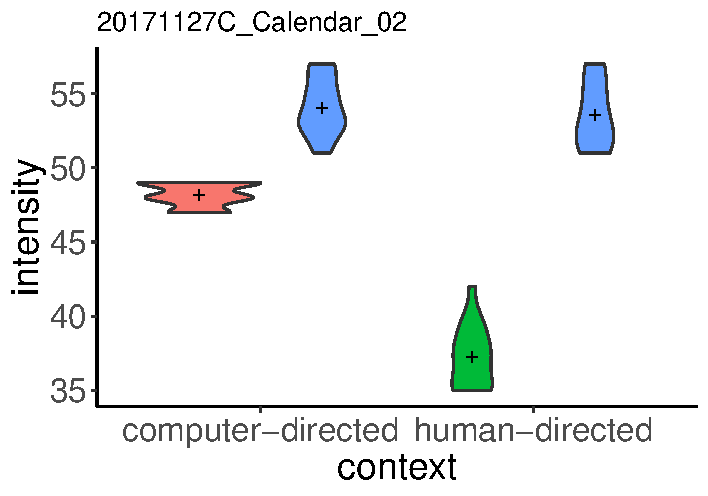
\includegraphics[width=\linewidth]{20171127C_Calendar_02_intensity_violin}
	\caption[An interaction with insignificant \acs{hds} and \acs{dds} intensity distributions difference]
		{An example of \ac{hds} and \ac{dds} distributions with a \emph{insignificant} difference (p-value~=~0.55, $\alpha=0.05$) extracted from the intensity measures of participant 20171127C in the calendar task.
		A significant example is presented in \cref{fig:hds_dds_violin_signif}.
		The colors represent distributions of Alexa (red), the confederate (green), and the participant (blue).
		The width of the box represents the frequency of the values and the \enquote*{+} sign marks their respective means.}
	\label{fig:hds_dds_violin_nonsignif}
	\todo[inline]{legend and units for y-axis}
	\todo[inline]{explain in text that comparison is only relative between two blue components}
\end{figure}
%
The differences between \ac{ar} distributions in \ac{hds} and \ac{dds} were calculated as well.
In \SI{13}{\percent} of the cases out of the 54 analyzed interactions the difference of means of the participant's \ac{hds} and \ac{dds} \ac{ar} distributions was significant.
This shows that the participants largely spoke with the confederate at the same speed as the device.
It was found that the articulation rate was lower in some specific cases where the participant tried to improve intelligibility, specifically when the system's output indicated that it could not understand the participant's previous utterance.
%While such utterance-level changes are interesting and may point to a temporary change in behavior, a more detailed analysis is outside the scope of this study, which concentrates on interaction-level behavior.
%
\begin{table}[t]
	\centering
	\caption[Percentage of significantly different interaction pairs in addressee component]
	{Percentage of interaction pairs with significant differences with respect to each target feature with all the interactions together and separated by order tasks.}
	\label{tab:signif_conditions}
	\sisetup{table-format=3.0}
	\begin{tabularx}{\linewidth}{XSSS}
		\toprule
		\thead[l]{feature} & {\thead{any order}} & {\thead{solo first}}	& {\thead{confederate first}}\\
		\midrule
		\acs{f0}	& 67	& 72	& 60 \\
		intensity 	& 67	& 76	& 56 \\
		\acs{ar}	& 30	& 31	& 28 \\
		\bottomrule	
	\end{tabularx}
\end{table}
%
\begin{figure}[t]
	\centering
	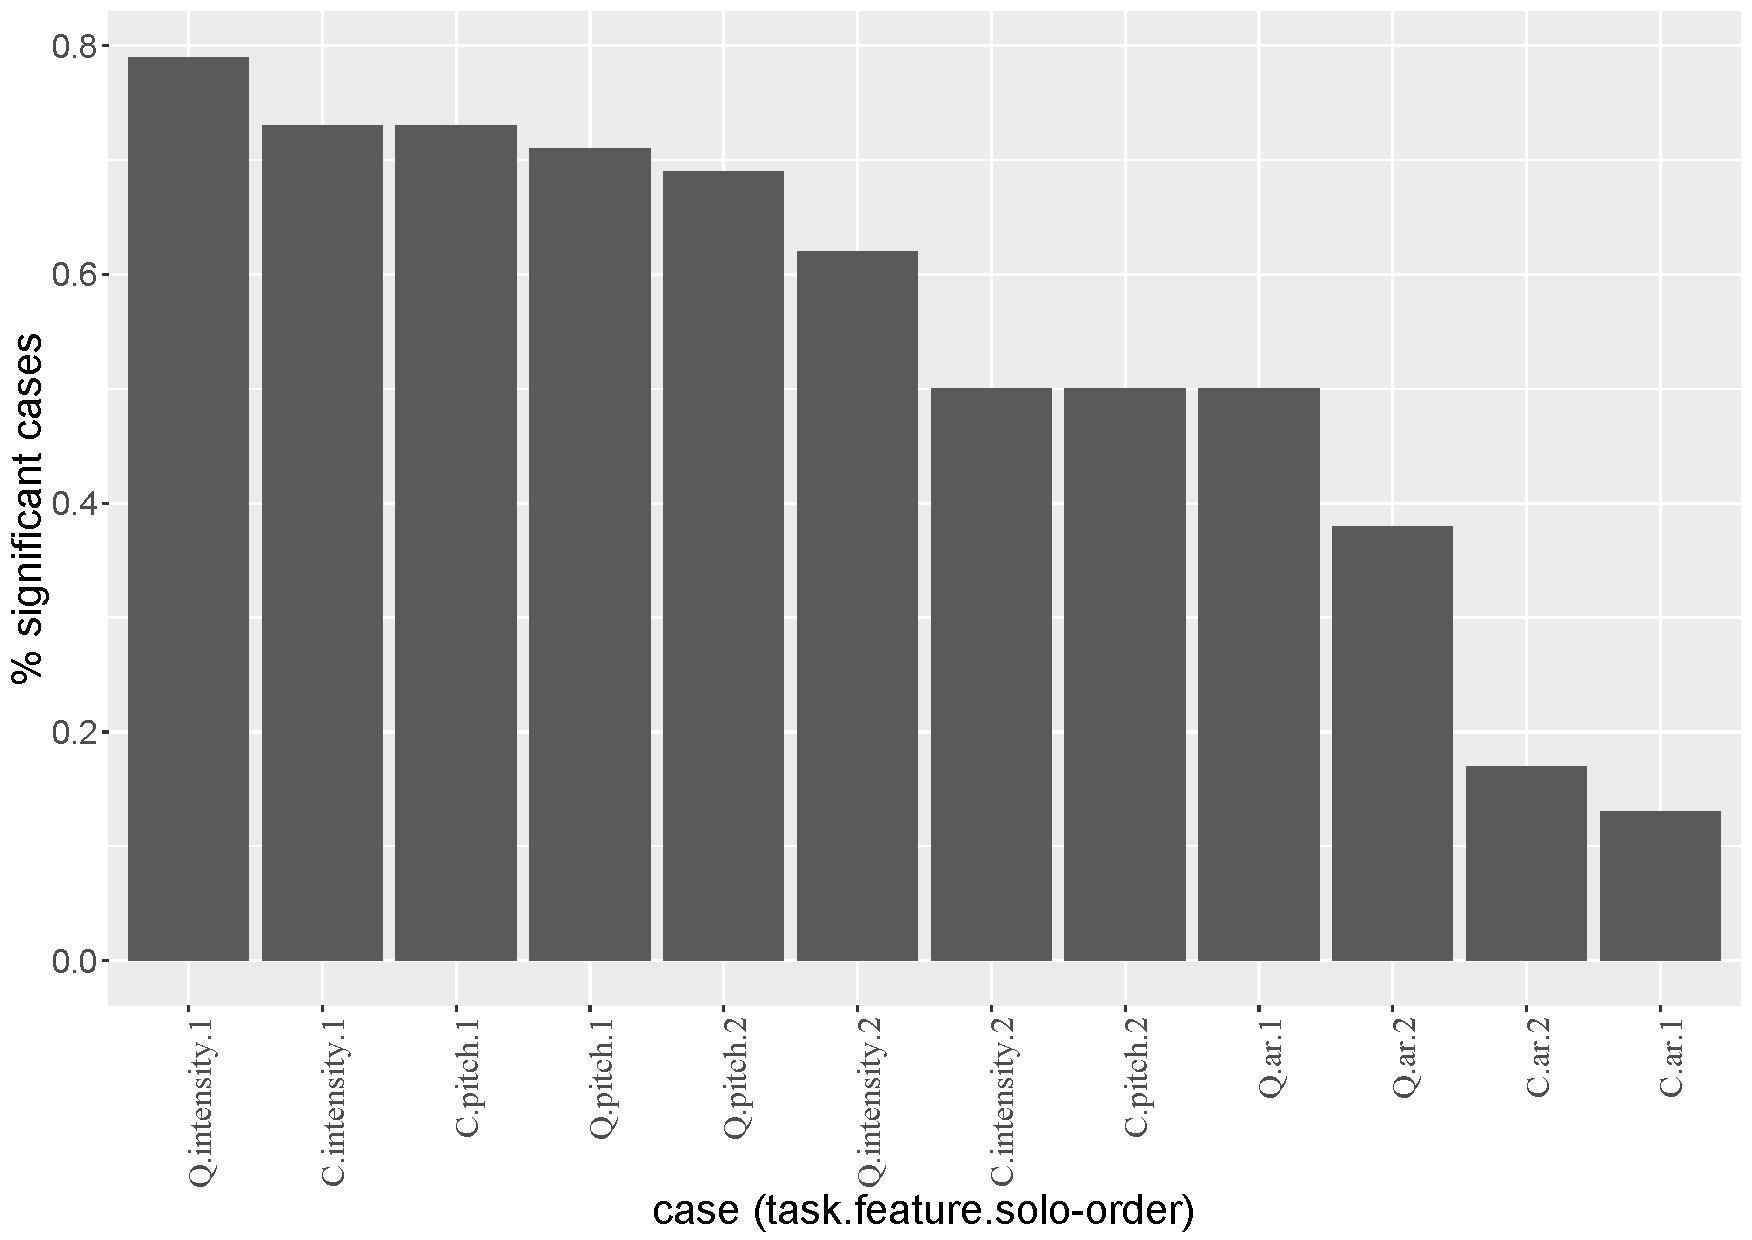
\includegraphics[width=\linewidth]{barplot_signif_cases}
	\caption[Per-case comparison of significant distributional differences in the crowd component]
		{Percentage of instances with a significant difference between solo and confederate conditions in each case.
		A case is a combination of the factors \emph{task}, \emph{feature}, and \emph{order}.
		For example, the case \emph{Q.intensity.2} contains the comparisons of intensity in interactions of the quiz task where solo condition was performed second (and the confederate condition first).}
	\label{fig:signif_cases_ordered}
\end{figure}
%
\begin{figure*}[t]
	\centering
	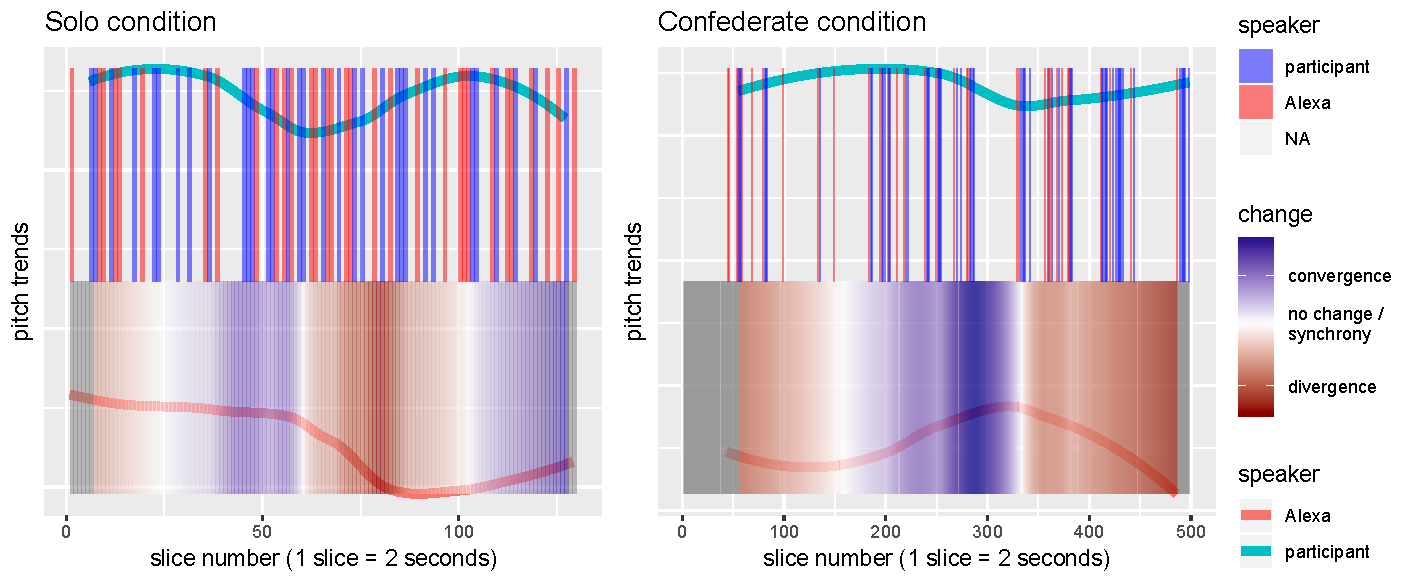
\includegraphics[width=\linewidth]{20171127B_Quiz_pitch}
	\caption[Temporal comparison of accommodation in solo and confederate conditions]
		{A comparison between the behavior of the \ac{f0} feature in solo condition (left) and confederate condition (right).
		The lines represent the \ac{loess} smoothing trend lines of the participant (blue) and Alexa (red).
		Omitted turns, e.g., turns of the confederate and turned removed as explained in \cref{sec:method} are not colored (gray).
		The vertical bars in the upper half represent the turns of the participant (blue) and Alexa (red).
		The color-scaled vertical bars at the bottom half are the convergence/divergence level of the participant over time as calculated in \cref{eq:accommodation}.
		Blue areas represent convergence while red areas represent divergence.
		The darker the color, the greater the effect, with white color pointing to points of no change (or synchrony, in segments with both trends moving the same way).}
	\label{fig:condition_convergence_comparison}
\end{figure*}
%

The distributional analysis examines the differences between the participant and Alexa's speech in solo and confederate conditions in terms of the general behavior of the participants with respect to the target features.
This general behavior is determined by the set of values of the target features produced by the participants in each condition.
Since this analysis checks whether the participants behave differently as a whole towards the non-human speaker, the temporal order of the values is not considered.
To detect these differences, the distribution of their respective values in the solo and confederate conditions in each interaction pair were compared.
This was done by using the two-sample Wilcoxon test \citep{Wilcoxon1945individual}, with $\alpha = 0.05$ with the null hypothesis that similar distributions of the target feature were used in both conditions.
A significant result of the test means that the participant produced the respective feature differently when interacting with Alexa alone compared to when the confederate participated as well.
\cref{tab:signif_conditions} shows the percentage of interaction pairs, in which the null hypothesis was rejected, i.e., that the feature was utilized differently by the participant in each condition.
Since chronologically, by design, one of the conditions needed to precede the other, the percentages were also calculated separately for the cases where tasks were performed first in the solo condition (and then in the confederate condition), and vice versa.
This separation shows whether interacting first with Alexa alone, without any human input, influenced the vocal behavior of the participants.
As there were no breaks between the interactions, the only factors for change were the order of the conditions and the involvement of another human speaker.
Indeed, the percentages of significant differences when interacting first only with Alexa were higher by \SI{12}{\percent}, \SI{20}{\percent}, and \SI{3}{\percent} for \ac{f0}, intensity, and \ac{ar}, respectively.
\cref{fig:signif_cases_ordered} further breaks down the differences between interaction pairs and introduces the factor of the performed task.
In line with the tendency shown in \cref{tab:signif_conditions}, the features \ac{f0} and intensity have the highest percentages of significant cases, regardless of the performed task, and the tasks performed first show higher percentages of different distributions.
In the lower percentages, it is the task, rather than the target feature, that shows differences between the cases.
And last, for \ac{ar}, with the lowest percentages, there is a clear difference between the quiz and the calendar tasks.
All in all, the \emph{task} factor was a good indicator only for the feature with the lowest difference percentage and the \emph{order} factor was more informative for the features with higher percentages.
To sum up, these results show significant differences in the majority of the cases for two of the three features for both the addressee and crowd components.
These outcomes provide a look into further aspects of \ac{hds} and \ac{dds} and speech-related features in conversation analysis, which may help studies in topics like addressee detection or  multiparty \ac{hci}.

\subsection{Temporal analysis}
\label{subsec:temporal_analysis}

Looking at the distribution differences of the selected features in \ac{hds} and \ac{dds} sheds light on the general speech behavior tendencies.
However, this analysis leaves out an important aspect of spoken interactions, namely the time dimension.
While the interaction-level distributions measures show the overall range and frequency of the values, temporal analysis adds the information as to how they changed over time.
Adding the time dimension gives an overview of the interaction's structure and reveals fine-grained information regarding its characteristics, such as turn lengths, turn switching, pauses, the density of a speaker's utterances, accommodation effects, and more.
For example, \cref{fig:hds_dds_time_pitch} shows a case where the absolute \ac{f0} values are roughly the same in \ac{hds} and \ac{dds}, around \SI{150}{\hertz}, but the behavior of the participant is different.
In the \ac{dds} context, the participant generally keeps a stable distance from Alexa's voice, whereas in the \ac{hds} context the \ac{f0} values are closer to the confederate.
In both contexts, the participant's \ac{f0} starts around \SI{150}{\hertz}, but in \ac{hds} the minimum \ac{f0} is only slightly below this initial value, whereas in \ac{dds} it drops as far as \SI{25}{\hertz} lower.
A similar example of the intensity feature is shown in \cref{fig:hds_dds_time_intensity}.
Unlike the previous example, here the absolute values steadily differ by about \SI{5}{\decibel}, but the overall change is similar.
That is, in both cases the intensity rises from the beginning to around a quarter of the interaction's duration, and then decreases again until the end (in \ac{hds} more quickly than in \ac{dds}) down to approximately the same value as at the beginning.

Since \cref{fig:hds_dds_time_comparisons} shows two examples of the quiz task performed by two different participants, it is possible to compare the structure of these interactions as well.
As described in \cref{sec:vacc}, the quiz task in the confederate condition is designed so that the two human speakers need to find an effective way to solve the questions using Alexa.
After improving their strategy, the lead should ultimately be taken by the participant, who interacts with Alexa to solve the questions as quickly and correctly as possible.
In both examples, the interaction starts with relatively short turns and rapid context changes.
This might be ascribed to the fact that the participant is still trying to figure out the best way to interact with Alexa and the confederate.
Then, sometime after the middle of the interaction, there is a larger block of \ac{dds}, followed by some more turns of \ac{hds}, possibly discusses with the confederate about ways to solve the last questions.
Finally, the interactions end with a shorter block of \ac{dds}, in which the participants finish these last questions of the quiz.
This structure was found to be the typical flow of the quiz task across participants.
%
\begin{figure}[t]
	\centering
	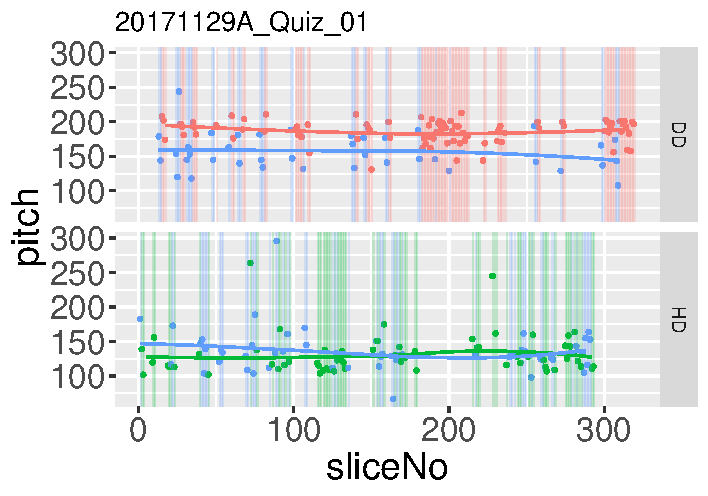
\includegraphics[width=\linewidth]{20171129A_Quiz_01_pitch_time}
	\caption[Comparison of temporal \acs{f0} trends of \acs{hds} and \acs{dds}]
		{The changes of intensity over time in \ac{dds} (upper part) and \ac{hds} (lower part).
		The timespans on the x-axis are represented by turn slices, as explained in \cref{sec:analysis_hhci}, and the y-axis shows the value of the feature.
		A slice's background color indicates the speaker in this slice and the circle with the same color, the measured value of the feature in it.
		Alexa's voice is shown in red, the confederate in green, and the participant in blue.
		The lines are smoothed values calculated by LOESS \citep{Cleveland1988locally}.
		In \ac{dds}, the speaker starts a bit above \SI{150}{\hertz} and ends slightly beneath it, generally maintaining the distance from the device's values.
		In \ac{hds}, the contour starts around the same value as in \ac{dds}, but gradually goes down towards the confederate and then up again, staying in the same range of values as the human speaker.
		This shows a different behavior with similar values.}
	\label{fig:hds_dds_time_pitch}
\end{figure}
%
\begin{figure}[t]
	\centering
	{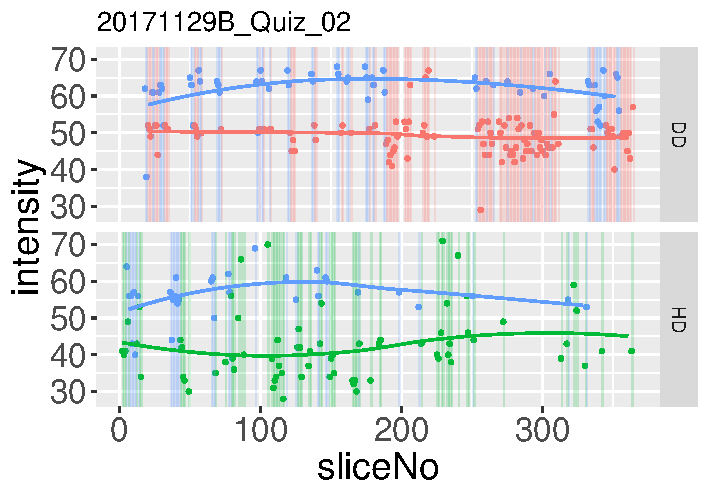
\includegraphics[width=\linewidth]{20171129B_Quiz_02_intensity_time}
	\label{fig:hds_dds_time_intensity}}
	\caption[Comparison of temporal intensity trends of \acs{hds} and \acs{dds}]
		{The changes of intensity over time in \ac{dds} (upper part) and \ac{hds} (lower part).
		The timespans on the x-axis are represented by turn slices, as explained in \cref{sec:analysis_hhci}, and the y-axis shows the value of the feature.
		A slice's background color indicates the speaker in this slice and the circle with the same color, the measured value of the feature in it.
		Alexa's voice is shown in red, the confederate in green, and the participant in blue.
		The lines are smoothed values calculated by LOESS \citep{Cleveland1988locally}.}
		In both \ac{hds} and \ac{dds} contexts, there are a rise and a fall around the same time in the participant's values.
		However, the absolute values differ.
		This shows a similar overall behavior with different values.
	\label{fig:hds_dds_time_comparisons}
\end{figure}
%
\begin{table}[t]
	\centering
	\caption[Percentage of significantly different interaction pairs in crowd component]
		{Summary of results. The percentage of interactions in which the difference of distribution means was significant for each feature, and their mean and \acf{sd}.}
	\label{tab:results_hhci_addressee}
	\begin{tabularx}{\linewidth}{XSSS}
		\toprule
		& \acs{f0} 						& {intensity}				& \acs{ar}									\\
		signif. diff.					& \SI{74}{\percent}			& \SI{89}{\percent}		& \SI{13}{\percent} \\
		\acs{hds} mean (\acs{sd}) 		& 10.5\,\si{\hertz}			& 2.95\,\si{\decibel}	& 0.627				\\
		\acs{dds} mean (\acs{sd}) 		& 10 \,\si{\hertz}		& 2.61\,\si{\decibel}	& 0.634				\\
		\bottomrule	
	\end{tabularx}
\end{table}
%	
Another way to look at accommodation in an interaction is in the temporal dimension.
In this analysis, the same raw measured values were used to examine changes that occur over time.
That is, unlike the analysis presented in \cref{subsec:distributional_analysis}, here the order of the values (i.e., their change over time) plays a major role, and effects may be found in specific time windows.
To perform such an analysis over the entire interaction, two additional computation steps are required.
First, each point in time must have a corresponding value for each feature produced by all speakers.
This was achieved by smoothing the measured value using \ac{loess} \citep{Cleveland1988locally}, a non-parametric regression method that deterministically fits a function to a localized subset of the data.
The fitting was done for each speaker separately over all slices of \ac{hds}/\ac{dds} with measured values of the features.
This results in a predicted value for each slice of the conversation.
\cref{fig:condition_convergence_comparison} shows an example of these smoothed measures of one participant and Alexa for the \ac{f0} feature.
The lower part of the figure shows the accommodation changes of the participant during the interaction (blue for convergence and red for divergence), and the upper part shows the turn-taking events.
The confederate condition has fewer turn events, as the analysis concentrates on the participant and Alexa, and the confederate turns are not shown.
Secondly, the relationship between a feature's values in each slice needs to be determined to describe their temporal changes.
Since we are interested in accommodative behavior, a measure for the relative change between slices was used.
It calculates the participant's contribution to the overall change in proximity between the participant and Alexa.
Alexa's contribution is considered to be a static effect, as it is not directly changing based on the user's speech input, and is therefore not taken into account.
The change tendency between two slices is calculated by
%
\begin{equation}
	\label{eq:change}
	change_t = -\Delta_{t, t-1} \mid S_{part} - S_{Alexa} \mid,
\end{equation}
\eqname{Smoothed change tendency of two interlocutors}\noindent
%
where the index $t$ refers to the current slice and $S_{part}$ and $S_{Alexa}$ are the smoothed values of the participant and Alexa, respectively.
The minus sign at the front flips the value so that increased proximity (convergence) is represented by positive values and distancing (divergence) by negative values (see \cref{fig:condition_convergence_comparison}).
Subsequently, the participant's contribution toward the accommodation is calculated by
%
\begin{equation}
	\label{eq:accommodation}
	accomm(participant)_t = change_t - \Delta_{t, t-1} S_{Alexa}.
\end{equation}
\eqname{Speaker's own contribution to mutual accommodation}\noindent
%
The sum of the proximity changes of each target produced by all participants in every sex-task-condition-order combination was calculated, resulting in a single value that represents the overall change.
A value greater than zero means that more convergence was observed, and a negative value points to more divergence.
There were only two instances where this value was exactly zero, both for the \ac{ar} feature.
These instances were treated as cases of divergence, for their divergence spans were longer.
Using this approach, only a few interactions had no feature convergence in them, and several had all three features showing convergence.
However, a stricter approach was applied, where a feature was considered as converging only if its overall accommodation value was higher than one standard deviation from its mean.
Based on that, all interactions were categorized by the number of features that showed more convergence in them.
\Cref{fig:alluvial} summarizes the categorization for each factor individually.
Each line represents a single interaction.
The strata labels through which each line passes, indicate the group it belongs to with respect to each factor.
The number of features that showed more convergence than divergence overall is marked by the color of the line.
Some tendencies emerge from this categorization:
first, in \SI{35}{\percent} of the interactions, there was at least one feature that showed convergence, but in none of them did all three features do so.
In seven interactions, two features showed convergence, twice by males and five times by females.
In total, males converged in \SI{5}{\percent} of all measurements and females in \SI{7}{\percent}.
Furthermore, of all the instances of converged features, \SI{58}{\percent} occurred in the solo condition, compared to \SI{42}{\percent} in the confederate condition.
However, no difference between the calendar and quiz tasks was found, with \SI{49}{\percent} and \SI{51}{\percent} of the cases, respectively.
The same holds for the comparison between the two orders in which the tasks could be performed.
These results support the addition of the confederate to the interaction as the factor for less convergence.
%
\begin{figure}[t]
	\centering
	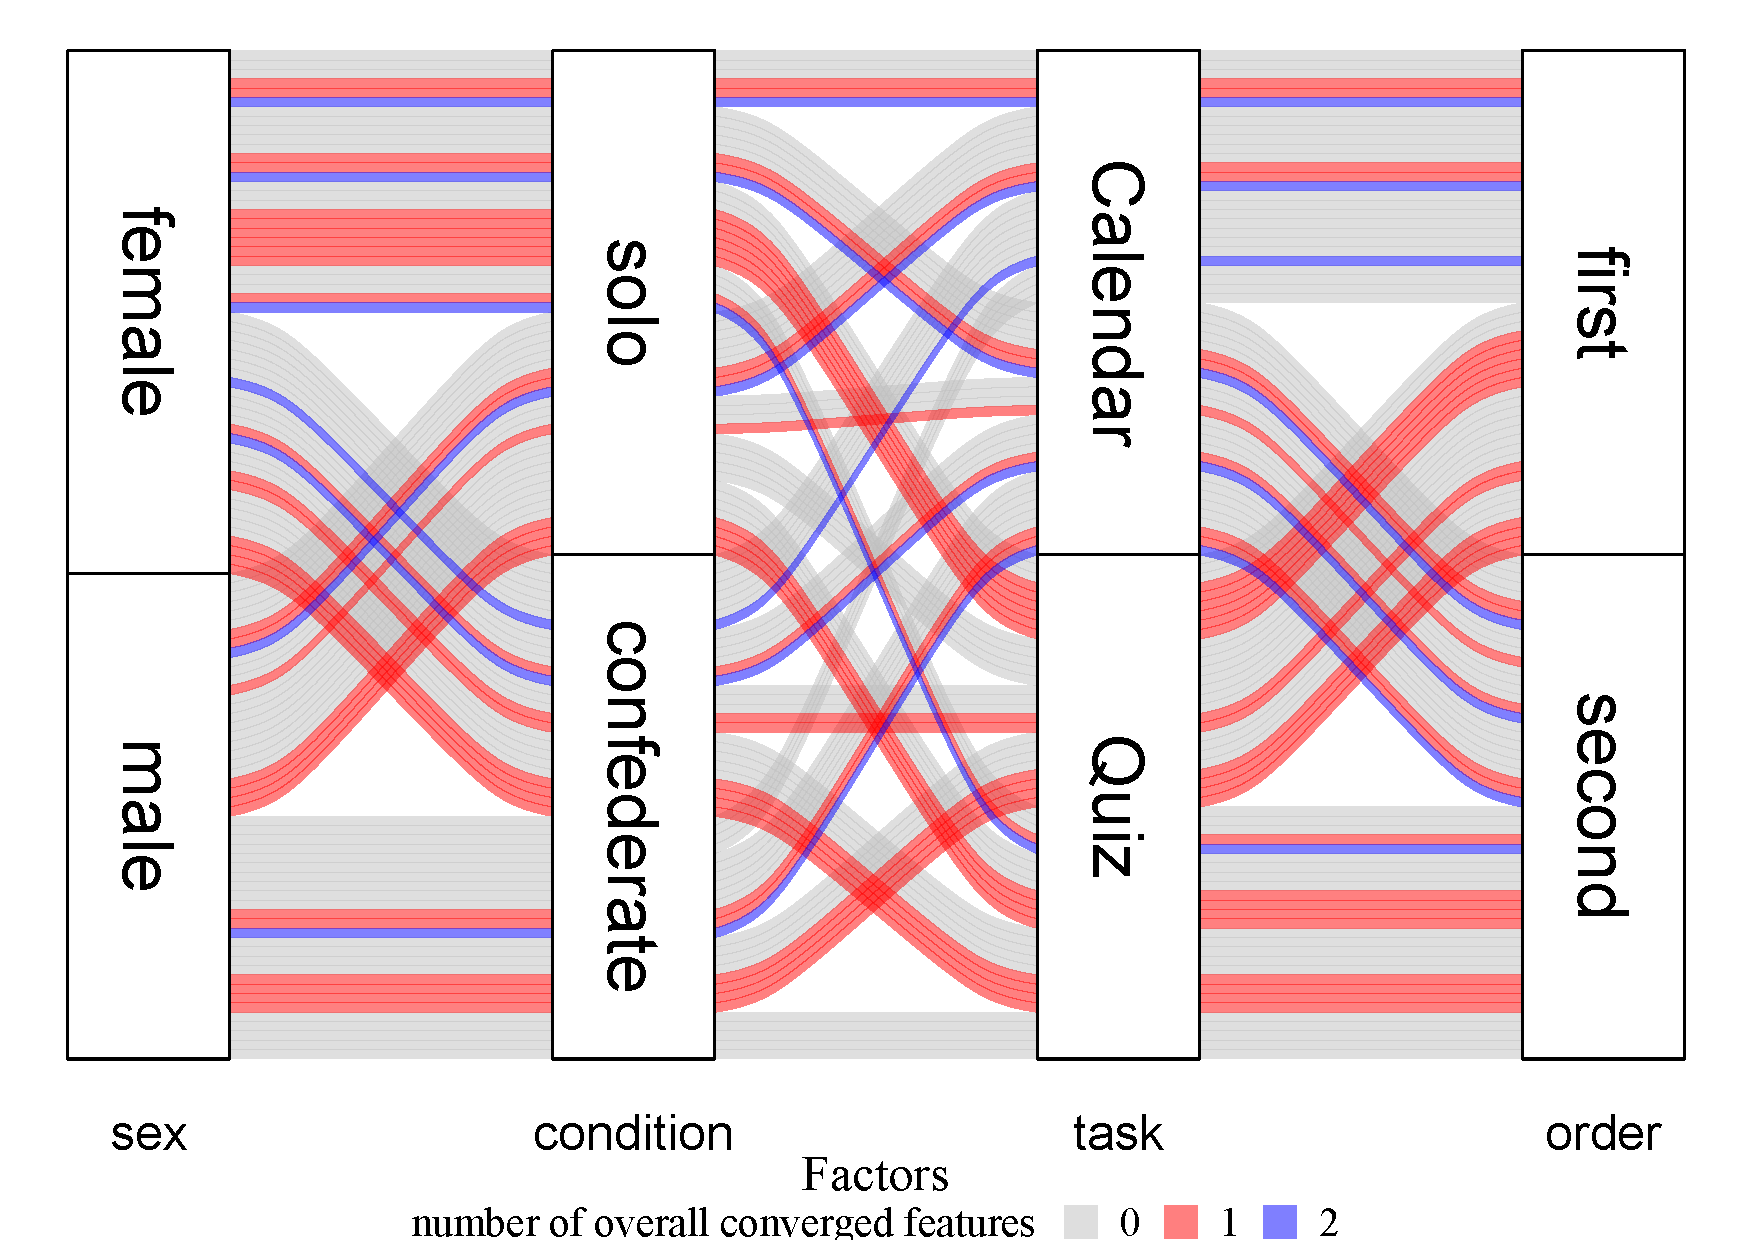
\includegraphics[width=\linewidth]{alluvial_4factors_numConv_strict}
	\caption[Number of significantly different behaviors per factor]
		{Overview of the relation between the factors \emph{sex}, \emph{condition}, \emph{task}, and \emph{order} and the number of features that showed more convergence in total across the interactions.
		Each line represents one interaction.
		The \emph{sex} stratus refers to the sex of the participant, and the \emph{order} stratus to the position of an interaction in the order in which the task-condition combination was performed.
		The color of a line stands for the number of target features that showed overall convergence in this interaction, from none (zero features, in gray), through one (red), and up to two (blue).
		%		and up to all three features (green).
		For example, a blue line going through the strata sequence female $\rightarrow$ solo $\rightarrow$ quiz $\rightarrow$ first represents an interaction with a female participant performing the quiz task in solo condition first, where the participant converged in two out of the three target features.}
	\label{fig:alluvial}
\end{figure}
%
\section{Discussion}
\label{sec:discussion}

\emph{Addressee} and \emph{crowd} components examined different aspects of a simulated real-world use case, in which a human user talks alternately with a computer-based interlocutor and another human interlocutor.
\cref{sec:accommodation_in_multiparty_interaction_with_an_agent} introduces this modern-day means of communication and where it occurs.
Distributional and temporal accommodation analyses were performed for these components to provide interaction-level and time-sensitive insights.
Results for the three target vocal features, \ac{f0}, intensity, and \ac{ar}, are presented in \cref{sec:results_hhci}.

On the component level, the first two features show a greater degree of difference in both components, and the latter, a smaller one.
Furthermore the changes are even larger in the crowd component, in which a human interlocutor is involved, than in the addressee component.
This indicates that \ac{f0} and intensity are generally more prone to variation than \ac{ar}, and hints that human interlocutors trigger these variations more.
There might be two reasons for this difference.
First, computer-based agents, including Amazon Alexa, do not change their speech output in any way, regardless of the user's input and variation in it.
As a social, dynamic, mutual process, accommodation is more likely to be stronger if both interlocutors contribute to the overall effect.
In this experiment, the process can only be mutual in \ac{hds}, where accommodation may occur naturally (cf.\ \cref{sec:communication_accommodation_theory}).
Secondly, due to this natural, spontaneous nature of accommodation in \ac{hhi}, the participants probably automatically spoke differently, more dynamically, in \ac{hds}, since the expectation for similar variation and dynamics is inherently expected from a human interlocutor.
Finally, \acp{va} (and voice-activated devices as a whole) are, in most cases, still not performing well enough for people to speak to them as fluently and dynamically as with other humans.
This has technical reasons, but the result is a different consciousness while talking to machines.
For example, users are more likely to articulate whole sentences, typically without reformulating, when requested to repeat their utterance by the device, whereas human interlocutors are capable of requesting and conveying corrections for shorter segments of utterances using intonation and other means.
Furthermore, although generally more seldom vary, users tend to reduce their \ac{ar} when repeating their utterances to the device, or when trying to be more clear.
This resembles the way people talk to children when they want to be more clear.
However, due to the way \ac{asr} systems are trained, more often than not this achieves the opposite result.
This reduced speaking rate phenomenon is discussed further below.

Regarding the individual features, one possible explanation for the different \ac{f0} distributions is the natural difference in male and female \ac{f0} (Alexa used a female voice while the confederate was always male), which leaves room for accommodation for participants of both sexes.
In that case, the results shown here point to the fact that the participants generally treated Alexa as a human interlocutor with regards to \ac{f0} behavior, as opposed to, for example, matching only the human interlocutor and talking to the computer-based interlocutor using the same, somewhat monotonous \ac{f0}.
A similar effect was found for intensity.
Since the device and the confederate were spaced approximately at the same distance from the participants, there was no apparent reason for the participants to speak more loudly with either interlocutor.
Therefore, an explanation of the tendency to speak more loudly to the device may come from the intuition that a computer-based system has a harder time understanding human speech and therefore needs a clearer signal.
This stands in line with the interpretation presented above that humans sometimes treat voice-activated devices as humans who need a hyper-articulated signal, e.g., toddlers or language learners\footnote{In a sense, this analogy is correct, as the devices -- or rather their \ac{asr} components -- indeed learn to process speech signals.
Despite that, this process is not identical to the way babies learn this, and therefore such projection on the speech style does not help the device improving its understanding of the user.
The technical and psychological differences and consequences of that are beyond the scope of this chapter.}.
Another explanation may be the illusion that Alexa feels more distant than the human interlocutor because she is not an embodied agent \citep[cf.][and see \cref{sec:types_of_sdss} for further details]{Staum2010virtually, Gijssels2016speech}.
Keeping in mind that an interaction aims to be as efficient as possible using minimum effort, it seems like changing these features helped the participants -- or at least felt like they did -- to interact more efficiently with the device.
Regardless of whether this roots from the unconscious attempt to treat the device like a human interlocutor or the fact that accommodation occurs, even if to a lesser extent, even when not mutual, the effect still takes place.
This is, however, not the case with \ac{ar}, which shows a lower percentage of significant differences.
This indicates that \ac{ar} does not tend to vary as much as \ac{f0} and intensity, which stands in line with other studies, like \citet{Schweitzer2013convergence}.
Slower, more carefully articulated speech, occurs less often in regular speech than louder speech or higher pitch.
Such enhanced articulation not only takes longer to produce, but also requires more effort, making it a less preferred way to communicate, unless necessary.
In this somewhat formal, experimental setting, participants are likely to speak more slowly than usual, and the motivation to complete the task in a short time does not encourage them to speak even more slowly.
This supports the hypothesis that extra slow speech would only be used when necessary, e.g., when a repetition is required due to a misunderstanding of an utterance, as discussed above.
Even in that case, the overall \ac{ar} tends to increase afterwards, to make the interaction more fluent again.
These local, short-term variations may suggest that changes in \ac{ar} are done more consciously than in other phonetic features.

The results presented in \cref{tab:results_hhci_addressee,tab:signif_conditions} show that for all three features
\begin{enumerate*}[(a)]
	\item the distributions differed more when the participants first interacted with the device alone, and
	\item more convergence was aggregated in the task that was performed first.
\end{enumerate*}
Furthermore, the factors \emph{sex} and \emph{task} indicated that female participants showed less convergence than male participants, but the task performed did not play any role in increasing the amount of convergence.
The first speech input a participant encounters may cause a priming effect that, together with the natural tendency to converge to an interlocutor, results in a greater change in interactions that occur first.
However, the interchangeability of input (here, both \ac{hhi} and \ac{hci}) seems to hinder the ability of the participants to converge to Alexa.
One explanation for this may be that it is more natural for humans to accommodate to other humans, so once another human is involved, the accommodation towards the computer interlocutor is neglected.
Another possible explanation is that due to the multiple interlocutors, the participants do not have a steady target towards which to accommodate, which leads to a weakened convergence effect.
This is confirmed by the higher rate of convergence in the solo condition compared to the confederate condition.
Since \ac{hci} still lacks the mutuality of a comprehensive accommodation effect, the question arises whether these tendencies would be stronger in interactions with a single human versus interactions with two different human speakers simultaneously.
The higher number of convergence instances by female participants may be ascribed to the \ac{va} using a voice of the same sex and could be further investigated by using a \ac{va} with a male voice.
Temporal analysis showed higher degrees of alignment towards Alexa in the solo condition.
This could be explained as a reaction to a more stable vocal target (especially since Alexa generally doesn't change her voice much) than when speaking to two entities alternately.
From the collaborative point of view, this may also be due to the fact that the participants wanted to create better collaboration relations to improve effectiveness.
This is a natural, even automatic, process that occurs in \ac{hhi}, but of course does not affect, as for today, computer-based interlocutors.
In general it was clear that accommodative effects and tendencies were present in both conditions, which is reassuring for future multiparty \ac{hci} accommodation research.
Two main open questions remain concerning the temporal aspect of interactions.
The first has do to with analysis on the speech \emph{signal level}, where the changes in measures over time can capture phenomena like convergence or divergence.
In a more comprehensive analysis in this direction, more detailed patterns may emerge.
Such an analysis can concentrate on one context or on comparing patterns in both \ac{hds} and \ac{dds}.
Additionally, more features can be measured to reveal more details regarding speech behavior.
The second may highlight behavioral patterns of the conversation on the \emph{turn levels}.
This can include a closer examination of the interaction structure as a whole, the dynamics of turn changes, pauses and repetitions, etc.
Such an analysis can be performed on interactions in solo and confederate condition to inspect whether humans deal with the same task performed with a computer alone differently than when another human is involved.

\part{Modeling}
\label{part:modeling}

\chapter[Computational Model]{Computational Model}
\label{chap:computational_model}

\lettrine{F}{or} a computer to express accommodative speech, a machine-understandable description of the process is required.
This chapter introduces a model of the way accommodation occurs in human speech, represented as a pipeline.
Its steps' order and logic are motivated by observed empirical data and aim to resemble the process that occurs in humans.
The parameters used in the pipeline to shape vocal behaviors are explained as well.

\pagebreak

\section{From \acs{hhi} to \acs{hci}}
\label{sec:from_hhi_to_hci}

The experiments presented in \cref{part:experiments} show humans' accommodation behaviors in different \ac{hhi} and \ac{hci} settings.
Complementary to that, \cref{subsec:accommodation_levels} discusses ways to represent the various levels of accommodative behaviors in computers.
Since behavioral changes, as explained by \ac{cat} (see \cref{sec:communication_accommodation_theory}), happen naturally and often unconsciously in \ac{hhi}, it is not trivial to transfer them to computers, as they need defined rules and numeric representation to process.
Numeric values can be achieved by applying some measuring technique appropriate for each feature, like formant values for vowel quality or frequency for \ac{f0}.
Rules for different behaviors, however, cannot be directly constructed, due to the intuitive nature of this inherent phenomenon, but can instead be inferred from observed \ac{hhi} data.
For example, the results of the study described in \cref{chap:shadowing_in_sung_music_and_human_computer_interaction} reveal a high degree of variation across participants (\cref{subsec:results_hci}).
While this is expected, further examination of these variations uncovers some general properties that can be taken as a basis for characterizing the different changes.
The link between the measured raw values and systematic rules should be a machine-applicable equivalence of the accommodation process in humans.
Such parallelisms would need to model, for instance, the way humans percept the accommodation-prone sounds, how they interact with previous instances and the current internal state of the sound in question, and the cognitive process of the phonetic changes.
Therefore, such a model should include the perception of the phonetic features, representation of the state change of each feature in memory, and the realization of the changes during a conversation.
Since these steps are, dependent on each other, the computational model presented here is depicted as a pipeline, where each of its steps stands for one of the sub-actions mentioned above.

\section{Pipeline representation}
\label{sec:pipeline_representation}

As accommodation happens automatically and seamlessly in human interlocutors' cognition, it is hard to say what are the exact steps this process comprises.
Some key properties stand out when examining many occurrences in different interactions.
The pipeline presented here aims to capture these properties and offer a defined process of describing the changes.
The advantages of representing this process as a pipeline (as opposed to, e.g., a one-step, end-to-end conversion) is that each facet of the process can be interpreted and controlled separately (ass demonstrated in \cref{subsec:computational_model,fig:adaptation_module_pipeline}).
This enables combining and experimenting with different methods and implementations for each step while maintaining their independence of each other.
The ability to substitute a single step's logic without influencing ther others grants the freedom to experiment with different methods without losing the core principles of the accommodation process.
For example, the calculation method in the \textit{update} step can be changed or even replaced by a statistical model (as the one in \cref{chap:statistical_model}).
Note that although only speech-related features are discussed here, this pipeline could be used for describing changes in other types of features and modalities that can be translated to numeric representations, like lexical choices, linguistic complexity, eye gaze, emotional state, etc.

The proposed pipeline representation consists of the following five main steps, which are explained in detail in \crefrange{subsec:detect}{subsec:assign}:
%
\begin{itemize}[topsep=0cm, itemsep=-.1cm, wide=0cm, leftmargin=!, labelwidth=\widthof{\textbf{update}}]
	\item[\textbf{detect}] hear and identify a feature that can be changed, corresponding to a human ear's ability to notice such variations;
	
	\item[\textbf{filter}] decide whether the encountered feature's instance appears in a way that can trigger change, capturing the inherent detection of phonological context and rules in the language;
	
	\item[\textbf{store}] add the instance to the exemplar pool of this feature, representing the inventory that builds the internal representation of the feature;
	
	\item[\textbf{update}] update the feature's state, standing for the \enquote{recalculation} of the way this feature is perceived by the speaker; and
	
	\item[\textbf{assign}] apply and potentially limit the updated state, expressing the change in a speaker's production of this feature with the individual preference as to how far to go with a change.
\end{itemize}
%
The output of each step is the direct input for the next, except for cases where the execution is discontinued due to an unmet condition (see \cref{fig:adaptation_module_pipeline}).
%
\begin{figure}[t]
	\centering
	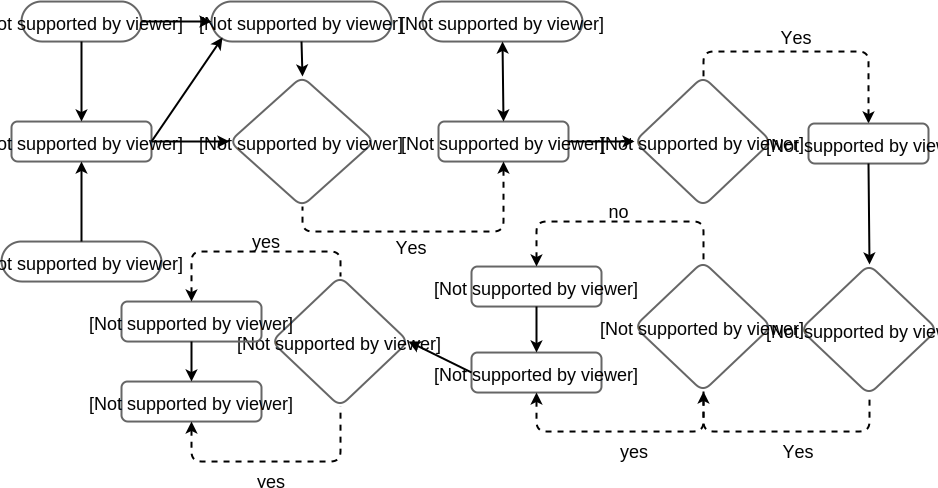
\includegraphics[width=\linewidth]{pipeline}
	\caption[Phonetic convergence algorithm pipeline]
		{Overview of the vocal accommodation pipeline.
		Rectangle nodes represent steps where an action is performed, round rectangles are inputs (either external or from the system), and diamond-shaped nodes stand for decision points.
		Nodes without a \enquote{no} edge indicate termination of the process at that point if their condition is not met (and therefore no accommodation occurs).
		The pipeline can only be successfully completed at the \enquote{Set feature's new value} node.}
		% However, if the \enquote{Add exemplar} action was performed prior to termination, the exemplar is not removed and will be taken into consideration the next time the pipeline is triggered for the feature with which it is associated.
		% The \enquote{feature definitions} come from the configuration file and can be changed by the user.}
	\label{fig:adaptation_module_pipeline}
\end{figure}

\subsection{Detect}
\label{subsec:detect}

This step stands for the human ability to identify phonemes in speech and analyze the way they are realized.
The input to this first step in the pipeline is the raw speech signal of the speaker and its output is a sequence of realizations that may contain phonetic changes.
The \ac{asr} component of the system is responsible for detecting these realizations and their timestamps in the signal.
With this information, various methods can be used to define and measure target features to take into consideration and pass forward.
\Cref{subsubsec:detecting_segment_exemplars} shows an example of such a definition and how it is used in a \ac{sds}.

An interlocutor cannot accommodate to features that are not present in a speaker's speech.
For changes on any level to happen, some pre-defined feature that is prone to change needs to be present and detected in the input speech stream.
Moreover, for the changes to register as a variation of a feature, the realization produced by the speaker must be prominent and distinctive enough to be perceived by the listener.
In the case of computers, that means a way to measure the difference between realizations and classify their distance from one another.
This difference can be categorical or continual, depending on the feature.
In addition, not only the features which introduce meaningful difference are language- and culture-dependent, but they might also differ based on the specific situation in which the interaction takes place.
For example, a segmental feature of a language where a phoneme can be realized in two alternative ways (as the allophonic alteration explained in \cref{subsubsec:target_features_HCIConv}) will probably be ignored by a speaker of a language where only one of these vowels exist in its repository.
In this case, the two vowels will simply be mentally merged into one, without causing any difficulties with comprehension.
Suprasegmental features, like \ac{f0} contour and \ac{ar}, occur globally across the speech signal and are more often cross-lingual.
Still, for a computer to be able to detect and track changes in those features, a way to measure and compare them is required.

\subsection{Filter}
\label{subsec:filter}

This step corresponds the human internal, often unconscious, linguistic knowledge, and how it is used to decide which detected realizations are valid new instances that will be stored in memory.
Its input is instances of a defined target feature detected in the previous step and it outputs those instances that should be stored as exemplars of their respective features.
\Cref{subsubsec:filtering_exemplars} demonstrates how a filter is applied based on a phonological rule and a feature definition with a target phoneme.

A target phoneme serves as an anchor for a rule that aims to capture a phonetic feature or a more evolved phonological rule.
For example, the German phonological rule of \textipa{[@]} elision at word-final \emph{-en} (as described by \cref{eq:schwa_elision_rule}) can be captured by the phoneme sequence /C\textipa{@n}/, where C represents a consonant (although in practice only a subset of the German consonants can be placed at this position).
The anchor phoneme is \textipa{[@]}, since this is the segment that is subject to the change, namely the length -- or complete absence -- of it.
therefore, for this phenomenon, the target phoneme would be \textipa{[@]} and the measured feature would be segment length.
Another target feature described in \cref{subsubsec:target_features_HCIConv} is \textipa{[e:]} vs.\ \textipa{[E:]} realization of the mid-word grapheme \emph{ä}, which is captured by the target anchor phoneme \textipa{[E]} in a non-final position of a word.
Any defined feature goes through two filters.
First, the phonological context of the detected sequence is matched against the one defined for the target feature; and secondly, the defined accepted value range that would make it an acceptable instance of that phenomenon, like \textipa{[@]} length between \SI{0}{\milli\second} and \SI{60}{\milli\second} or appropriate F$_1$ and F$_2$ values for the \textipa{[e:]} and \textipa{[E:]} vowels in the aforementioned features.
After applying these two filters, only those instances that truthfully capture the desired phonetic phenomenon are kept.
Another purpose of this step is to provide a way to integrate phonetic expertise to be used in the process.
This helps not only to be more accurate regarding language-specific knowledge, but also to prevent \ac{asr} errors to propagate further in the pipeline.

\subsection{Store}
\label{subsec:store}

\begin{figure}[t]
	\centering
	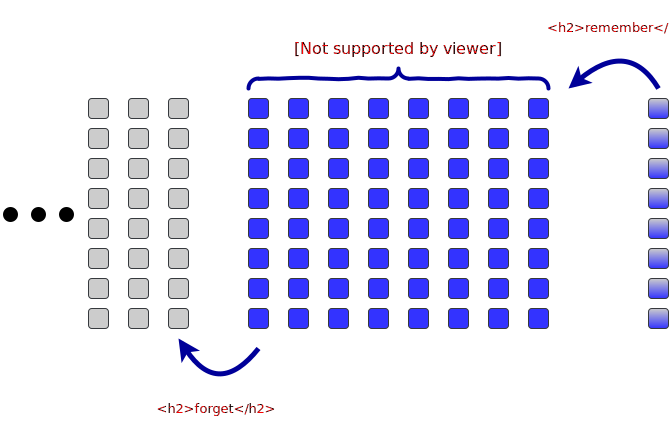
\includegraphics[width=0.8\textwidth]{pool}
	\caption[The exemplar pool]
		{Illustration of an exemplar pool.
		Each exemplar is represented by a column of squares (each representing a numeric value).
		A new exemplar is added to the feature's pool when encountered.
		Old exemplars are removed when the pool is full.
		Exemplars currently in the pool are taken into account when the realization of the feature is determined.}
	\label{fig:exemplar_pool}
\end{figure}
%
This step represents the mental phonetic memory of a speaker, here referred to as a \emph{pool} for a computer-based interlocutor.
The input to it is a feature's exemplars that passed the filtering step and its output is used for updating the feature's representation.
An illustration of an exemplar pool is shown in \cref{fig:exemplar_pool} and an implementation of it is described in \cref{subsubsec:collecting_exemplars}.

After an instance of a feature is detected and validated, it needs to be registered as an exemplar of the feature it is associated with.
This stands in parallel to the way such exemplars (and in other contexts also words, meanings, etc.) are mentally stored in the human's short- and long-term memories.
These accumulated exemplars of a feature determine how a speaker perceives it and shape its production when used in speech.
One of the complexities of modeling such internal representation is the interleaving influences of both long-term and short-term memory.
In spoken interaction, the long-term memory may define the typical productions of a user, while the short-term memory is used and changed within a single conversation.
Since this model aims to describe accommodation occurring within the scope of a single, isolated interaction (even if a long one), only the storage of exemplars encountered in this interaction is explicitly addressed in it.
However, long-term effects may be implicitly achieved by retaining values between interactions.
This step also defines how new exemplars are added, stored, and removed (cf.\ \cref{fig:exemplar_pool}).
Each feature has its own exemplar pool to which newly encountered exemplars are \enquote{memorized}, and each exemplar is a vector of the values measured for the target feature, e.g., formant values).
The pool functions in a first-in-first-out fashion, fitting the temporally linear progression of spoken interaction.
An exemplar is represented by a vector with cardinality $n$, where $n$ is the number of dimensions required for describing this feature.
Whenever an exemplar of the feature is encountered, a new exemplar is added to the pool.
The size of the pool determines the memory capacity, i.e., for how long exemplars are remembered during the interaction.
If the pool is already at full capacity, the oldest exemplar is \enquote{forgotten} when a new exemplar is added.
Ultimately, a pool of a feature can be used to determine which exemplars are still affecting the speaker's mental state of a feature.
As the order of the added exemplars is kept, it can be taken into account as well when determining each exemplar's weight, just like recent turns are more likely to influence the current utterance than turns from the beginning of the conversation.

\subsection{Update}
\label{subsec:update}

This step incorporates the process of changing the mental state of a feature based on its accumulated exemplars.
The input to it is the current state of a feature and it outputs a new value for it.

The core of the accommodation process is the change in a feature's state.
Many factors may influence this change, both internal and external.
The two main considerations in this step are one of each, namely the desired accommodation behavior and the exemplars collected from the user's speech input.
The latter is covered by the \enquote{store} step, and the former is defined using adjustable parameters that correspond to accommodation properties in humans (see \cref{tab:comp_model_parameters}).
For example, how prone is the speaker to be influenced by others' speech and how easily should the change be triggered.
The sensitivity can be constant or vary based, e.g., on how close are the speakers' productions to begin with.
A trigger might be exemplar-based, i.e., after a certain number of new exemplars were added, or time-based, i.e., every time a certain amount of turns had passed.
Another means to shape the behavior is the way the new state is computed based on the exemplars.
For example, newer exemplars or exemplars with greater distance from the current state may influence the change more.
Moreover, the general tendency to accommodate is defined in this step, e.g., converging or diverging from the user's speech, which is determined, among others, by the application and desired behavior.
A \ac{capt} system would probably not aim to align its speech to the user's, but rather diverge from it as a way to provide auditory feedback.
This computation can use simple mathematical operations (as demonstrated in \cref{subsubsec:calculating_changed_value}) or more involved data-driven statistical methods (as the one in \cref{chap:statistical_model}).

\subsection{Assign}
\label{subsec:assign}

This step mediates between the new state of a feature and its use in the system's speech output.
The input to it is the newly calculated state of a feature and it outputs a potentially altered version of this state to be used by the \ac{tts} component.

This final step of the pipeline is responsible for assigning the features' representations to the speech production of the system as an additional input to the system's \ac{tts} component.
For a \ac{tts} module that can directly control the speech output (as part of the model itself or on the outputted waveform, as discussed in \cref{subsec:speech_manipulation}),
this additional information can be used to manipulate the target features in a way that expresses the accommodative behavior of the system.
This closes the circle from a target feature produced by the user and up to the change it triggered in the system when it speaks back.
Since that means the user will now hear certain vocal characteristics that are based on their own speech, it is important to avoid a situation where the user feels imitated -- or even mocked -- by the systems.
This is an important issue that has not been considered in previous work.
To that end, this step introduces a limitation mechanism that limits the values given to the \ac{tts} component.
The values are re-evaluated if some threshold is bypassed (see \cref{eq:new_value}), to avoid such imitation from the system's side.
This mechanism also helps to prevent the system from diverging too sharply from the user.
For example, a \ac{capt} system might demotivate or frustrate the user if its speech is consistently considerably different from the user's.
From a human's perspective, this step corresponds to the natural degree to which a speakers would change their speech while talking to others.
As shown in \cref{chap:shadowing_in_sung_music_and_human_computer_interaction,chap:speech_variations_in_hhci}, this varies from feature to feature, and hence this parameter is set for each feature individually (see \cref{tab:comp_model_parameters}).
For this to work, it is important that the features are sufficiently distinguishable and clearly defined by the pipeline, so that the specified modification in the system's speech output can be properly applied in -- and only in -- the correct places, as illustrated in \cref{fig:adapted_synthesis_output}.
%
\begin{figure}[t]
	\centering
	\includegraphics[width=0.85\textwidth]{synthesis}
	\caption[Manipulated features on a synthesized waveform (illustration)]
		{Illustration of a manipulated output audio waveform.
		Each colored pin marks a phonetic features captured and processed by the pipeline.}
	\label{fig:adapted_synthesis_output}
\end{figure}

\section{Parameters}
\label{sec:parameters}

Several parameters are introduced into the pipeline described in \cref{sec:pipeline_representation} to grant degrees of freedom in shaping the accommodation behavior.
These parameters link between the theoretical, schematic model and its integration into a \ac{sds}, as demonstrated in \cref{chap:convergence_module_for_sdss}.
They are also the key to experimentation with different settings and scenarios for different applications.
The model's parameters are summarized in \cref{tab:comp_model_parameters} \citep[and cf.][]{Raveh2017Interspeech}.

\afterpage{%
	\begin{landscape}
		\begin{table}[t]
			\centering
			\vspace{1.5cm}
			\caption[Summary of computational model's parameters]
				{Computational model's parameters in their order of use.
				The colors mark parameters associates with the
				{\color{Violet}\textbf{detect}},
				{\color{BurntOrange}\textbf{filter}},
				{\color{ForestGreen}\textbf{store}},
				{\color{RoyalBlue}\textbf{update}}, and
				{\color{red}\textbf{assign}} steps.}
			\label{tab:comp_model_parameters}
			\begin{tabulary}{\linewidth}{lLL}
				\toprule
				\multicolumn{1}{c}{\textbf{Parameter}} & \multicolumn{1}{c}{\textbf{Description}} & \multicolumn{1}{c}{\textbf{Value}} \\
				
				{\color{Violet}\textbf{target phoneme}}*
				& the phoneme that triggers the feature's pipeline
				& a phoneme symbol\\\addlinespace[0.2cm]
				
				{\color{BurntOrange}\textbf{phonetic context}}*
				& the environment in which the feature instance is accepted
				& regex containing the of phoneme symbols containing target phoneme\\\addlinespace[0.2cm]
				
				{\color{BurntOrange}\textbf{allowed range}}*
				& the value range(s) in which new instances are accepted
				& two numeric values (min and max) per feature dimension\\\addlinespace[0.2cm]
				
				{\color{ForestGreen}\textbf{exemplar pool size}}
				& maximum number of exemplars in memory at a time, oldest exemplar removed when full
				& positive integer\\\addlinespace[0.2cm]
				
				{\color{RoyalBlue}\textbf{update frequency}}
				& how frequently a feature's value is recalculated, controlling the accommodation pace
				& non-negative integer; 0 for manual update\\\addlinespace[0.2cm]
				
				{\color{RoyalBlue}\textbf{calculation method}}*
				& the manner in which the pool value is calculated based on the values and order of the exemplars in pool
				& any $\mathbb{R}^{n \times m} \longrightarrow \mathbb{R}^{m}$ function; either implemented directly in code or sent to an external statistical model\\\addlinespace[0.2cm]
				
				{\color{RoyalBlue}\textbf{convergence rate}}
				& weight of the exemplar pool when updating the feature's state, controlling the impact of external input on the speaker's features states
				& real value; typically $n \in (0, 1) \subset \mathbb{R}$; 0 for ignoring the pool ; $> 1$ for over-weighting the pool value\\\addlinespace[0.2cm]
				
				{\color{red}\textbf{convergence limit}}*
				& the maximum degree of convergence allowed for the feature with respect to the input instances
				& real value; $n \in (0, 1] \subset \mathbb{R}$; 1 (\SI{100}{\percent}) for no limitation \\
				\bottomrule
			\end{tabulary}
			\flushleft{\footnotesize \emph{* denotes parameters that are defined individually for each feature}}
		\end{table}
	\end{landscape}
}

As shown in \cref{sec:convergence_to_natural_and_synthetic_stimuli}, not all participants showed the same \emph{sensitivity} toward changes in the stimuli.
Here, sensitivity refers to the degree of overall change toward external speech input.
Additionally, when one does converge, the sensitivity to changes (the \enquote{amount of differentiation}) toward a every single stimulus might differ as well.
These two aspects are jointly controlled by the \emph{convergence rate}, which represents the balance between the current and heard speech when calculating the accommodation outcome.
Generally, low convergence rate leads to a slow (and potentially unnoticeable) change, while a high rate would lead to sharper changes and that may overshoot the target, as demonstrated in \cref{tab:validation_baseline,fig:validation_sensitivity}.
To simulate the case where a speaker is not influenced by external speech input (the exemplars in the pool) at all, this rate can be set to zero.
In that case, the model will ignore the other interlocutor's speech and stick to the current speech style.
Another difference found among the participants was the total overall convergence degree toward the stimuli, i.e., where does the convergence process stop.
This is monitored by the \emph{convergence limit}, which defines the maximally allowed degree of similarity between the interlocutors.
When set to 1 (\SI{100}{\percent}), the model is allowed to change up to \SI{100}{\percent} toward the other interlocutor (complete convergence); when set to 0.8, up to \SI{80}{\percent}, and so on.
The parameter ensures that the model does not simply imitate the user's input, which is the approach often found in such system nowadays.
By limiting the change, the accommodation process is more gradual and restrained, avoiding peaks and abrupt changes.

Parameters defining the adaptation itself are not enough.
To properly model an accommodative behavior, some aspects that are not directly related to the speech output are required as well.
The accommodation process relies on the recent instances (\emph{exemplars}) of a speech sound.
How many exemplars are taken into account when the feature's state is updated depends on the interlocutor's mental memory of that sound.
This internal memory is a complex mechanism \citep{Baddeley2003working}, which is simplified here into a single parameter, namely the \emph{exemplar pool size}, which determines the number of exemplars the interlocutor currently remembers.
This exemplar history is managed on a first-in-first-out basis, so that the \emph{order} in which the exemplars were acquired is kept as well and can be used for weighting their influence.
This pool size can be tweaked to match the scenario and the expected interaction length.
The \emph{tendency to converge} toward other interlocutors also differs from speaker to speaker.
This likelihood is controlled by a parameter (a probabilistic approach for this property is discussed in \cref{chap:statistical_model}).
After an exemplar is added to a feature's pool, an update of the feature's value may be triggered.
Whether and how often this happens is determined by the \emph{update frequency}.
When set to 1, an update will occur every time an exemplar is added; if set to 2, every other exemplar, and so on.
When set to 0, however, updates will only take place when explicitly requested, e.g., after a pre-determined number of turns or a fixed amount of time.
This can be useful when all features are to be updated at the same time, regardless of how many exemplars have been accumulated for each of them.
Increasing the update interval means that each update will be affected by a higher number of new exemplars, which might result in a smoother converging process, depending on the calculation method used (see below).
Additionally, a longer update interval also means that accommodation will generally take longer, since the model's features are not being updated as frequently.
This is fitting for systems with which the user is expected to have long interactions.

Not only the frequency of updates plays a roll in the process, but also the manner in which the update is performed.
This manner is determined by the \emph{calculation method}.
Since the features in the model are represented by vectors, any function that takes a matrix as input and outputs a vector as output can be used, as demonstrated in \cref{subsubsec:calculating_changed_value}.
The method can be either statistical or deterministic, e.g., simply averaging the exemplars, but methods that can take order into account, like decaying average, might yield more realistic accommodative behaviors.
A different calculation method can be assigned to each feature, which can help to account for acoustic or psycholinguistic constraints.
This can also be influenced by the setting the system is purposed for, like experimental, exploratory, data collection, etc.

For each feature, a \emph{target phoneme} is defined, which has two purposes:
First, it tells the \ac{asr} component which phoneme is associated with this feature, so that it is forwarded for further analysis.
Secondly, it is used in the \emph{phonetic context} to filter instances of the phoneme that should not be associated with the feature.
The context is the environment in which the target phoneme should be found in the \ac{asr} output sequence for the instance to be considered\footnote{This requires an \ac{asr} engine that returns such a sequence in addition to textual output.
It is therefore crucial that the phoneme symbol set used in the model and by the \ac{asr} is the same and unambiguous, specifically when used in a regular expression.
This is the only part of the pipeline that is language-dependent (or rather symbol-dependent)
Using non-ASCII symbol sets, like IPA, may solve many of these issues, but is not recommended since \ac{asr} engines rarely use those and also due to other technical reasons.}.
For suprasegmental features -- or any other feature that is not bound to a specific phoneme or context -- the target phoneme can remain empty, so that the phonetic context would match any sequence.
The second parameter used to put constrains on the detected phones is the \emph{allowed range}, which defines the minimum and maximum acceptable values for the feature.
This parameter is important to obtain clean and sensible exemplars, as it introduces restrictions based on phonetic knowledge (e.g., reasonable \ac{f0} values for a human speaker), which at the same time also help to prevent \ac{asr} errors from meddling with the exemplars sent to the pool.
Since these values are feature-dependent, this parameter is set for each feature individually.
%\Cref{subsubsec:detecting_segment_exemplars} shows an example of a feature definition.
\chapter{Probabilistic Variational Model}
\label{chap:statistical_model}

\lettrine{I}{ntroduction} into this chapter\dots

\pagebreak

\section{Time series representation and \aclp{gp}}
\label{sec:time_series_analysis}

The approach presented here capitalizes on the temporal aspect of spoken interaction, specifically the evolution of the observed accommodation over the course of a conversation.
Hence, with the feature in question chronologically sampled along equal intervals in high temporal resolution, its values can be treated as a \emph{time series}.
Time series are used for both analysis and prediction in many field, like anomaly detection, econometrics, seismology, geophysics, and more.
Viewing accommodation as time series helps exploring it a process evolving over time and enables a range of analysis methods.
This approach is motivated by the arguments explained in \cref{subsec:temporal_analysis}, vis.\ that representing mutual changes by merely a few points throughout an interaction or directly comparing its beginning state to its end state is not very informative and draw a very simplistic picture (See \cref{subsec:limitations_of_did} and \cref{fig:accommodation_types} for more details about this motivation and the limitation of \ac{did} measures).

Whereas the computational model introduced in \cref{chap:computational_model} grants a \ac{sds} \emph{responsiveness} per the definition in \cref{subsec:accommodation_levels}, the approach here leads to a model that grants \emph{variability}.
It can also define a \emph{profile}, e.g., by taking the mean prediction as the core behavior (see \cref{fig:gp_vacc}), but this is not the goal pursued here.
Moreover, the generative model presented in \cref{sec:clustering_and_incremental_generation} can be combined with the aforementioned computational model, e.g., to limit the degree of accommodation or to control the change rate
This variability is achieved by fitting a \emph{\ac{gp}} to each speaker.
\Acp{gp} are stochastic processes with a multivariate normal distribution for each random variables.
Therefore, a \ac{gp} provides the joint distribution for infinitely many random variables, i.e., a \emph{distribution of functions} that match some given evidence.
Specifically \acp{gp} are used here for \emph{kriging} (\cref{subsec:interploating_data_using_kriging}), an interpolation technique, which is a technique used in application in various fields, like geostatistics, economics, and astronomy, to name a few.
The utilization of \acp{gp} provides not only a continuous line with likelihoods for the observed speech productions, but also an infinite number of potential alternatives -- the variations -- that describe the speaker's vocal behavior.

\subsection{Kernel building and tuning}
\label{subsec:covariance_functions}

\todo[inline]{current information taken from \url{http://scikit-learn.org/stable/modules/gaussian_process.html}. in the introduction add the reference(s) mention at the end of this page.}
\todo[inline]{also, there was a very detailed thesis/paper about kernels, check if there are more good details there}

Kernels (also called \textit{covariance functions} in the context of \acp{gp}) are a key in component \acp{gp}, as they define the statistical relationship between the input values.
In general, they represent describe the similarity $k(x, x')$ between each pair of input points, so that $k(\cdot, \cdot)$ determines how similar the outputs $y_*$ and $y_*'$ will be. 
More formally, a covariance function can be described as $\mathcal{K}(u, v) = \phi(u) \cdot \phi(v)$, where $\phi(\cdot)$ is a function that maps the input vectors into a transformed feature space.
Which function to use is a key question when modeling using a \ac{gp}, as it determines the behavior of the model and the quality of the predictions it will be able to make.
Naturally, some assumptions and decisions regarding the data must be made when choosing a kernel.
A kernel's parameters are optimized to achieve functions that better fit the data, the consistency of the resulted functions is measured using log maximum likelihood.

Since convergence analyses usually refer to the \textit{difference} between values in different production (as opposed to the values themselves), stationary kernels are more suitable for fitting \ac{gp} to them, as they are shaped by the distances between each pair of data point rather than merely their absolute values.
%That is, they fulfill $k(x_1, x_2) = k(x_1 - x_2)$.
%This list only covers a small subset of common covariance functions.
%Further kernels include the exp-sine squared, dot-product, linear, and more.
%\putref{put 2 references about kernels, or only 1 is the first is used above}
Kernels can also be chained using multiplication or addition to combine characteristics of multiple kernels.
Multiplication-based kernels are maximized when all of its kernel factors yield high values, whereas
addition-based kernels, are maximized when any of their addend kernels yield a high value.
%For example, multiplying a linear kernel by a periodic one will result in functions that are \textit{both} periodic \textit{and} with increasing amplitude as they move away from the origin.
For the modeling presented here, an additive kernel is used with constant, RBF, and noise terms (see \crefrange{eq:constant_kernel}{eq:RBF_kernel}).
The RBF term determines the general shape of the curve (see example in \cref{fig:RBF_prior_posterior}), the constant term enables shifting of the curve if necessary, and the noise term adds degrees of freedom in case the curve cannot completely fit the input signal.

The definitions of the individual kernels are as follows:

\begin{description}
	\item[Constant kernel -- ]
	This is a simple kernel that assigns the same value for all input pairs.
	Since by itself it does not offer a lot of characteristic to the covariance function, it is usually used as part of a product kernel, where which it scales the magnitude of the other factors, or as part of a sum kernel, in which it modifies the mean of the Gaussian process.
	It has a single parameter, the constant value, and it is defined as 
	%
	\begin{equation}
		\label{eq:constant_kernel}
		k_{constant}(C, x, x') = C\forall x_1, x_2,
	\end{equation}
	\eqname{Constant kernel}
	%
	where $C$ is the constant value parameter.
	
	\item[Noise kernel -- ]
	is a kernel used for capturing unexplained variation in the data, i.e., noise.
	It is typically based on the constant kernel as part of a sum kernel, in which it explains the noise component of a signal.
	In this context, the constant parameter is tuned to estimate the noise level.
	This is determined by
	%
	\begin{equation}
		\label{eq:noise_kernel}
		k_{noise}(\{noise\_level\}, x, x') =
		\begin{cases}
		C_{noise\_level}, & if\quad x_1 = x_2\\
		0, & otherwise,\\
		\end{cases}
	\end{equation}
	\eqname{Noise kernel}
	%
	where $noise\_level$ equals the variance of the noise found in the input signal.
	
	\item[Radial-basis function (RBF) kernel --]
	also known as \emph{squared exponential kernel}, the RBF kernel is a stationary kernel with one parameter, \emph{lengthscale} $l > 0$.
%	 which can either be a scalar (isotropic variant of the kernel) or a vector with the same number of dimensions as the inputs x (anisotropic variant of the kernel).
	This kernel typically results in generally smoothed functions, with the lengthscale being associated with the long-term smoothness and degree of variability on the time dimension.
	The RBF kernel is defined as
	%
	\begin{equation}
		\label{eq:RBF_kernel}
		k_{RBF}(\{\ell\}, x, x') = \sigma^2 exp\left(\frac{\lVert x_1 - x_2 \lVert ^2_d}{2\ell^2}\right),
	\end{equation}
	\eqname{Radial basis function (squared exponential) kernel}
	%
	where $\lVert x_1 - x_2 \lVert$ is the Euclidean distance between two $d$-dimensional input points and $\sigma^2$ is a scalar factor that determines the average distance of your function away from its mean.
	\cref{fig:RBF_prior_posterior} shows prior and posterior examples of the RBF kernel.
	
%	\item[Rational quadratic kernel]
%	This kernel can be seen as a scale mixture (infinite sum) of RBF kernels with different length scales.
%	Therefore, \acp{gp} priors with this kernel expect to see functions which vary smoothly across many length scales.
%	It has two parameters: length scale $l > 0$ and scale mixture $\alpha > 0$.
%	The parameter $\alpha$ determines the relative weighting of large-scale and small-scale variations.
%	When $\alpha$ $\lim$ $\inf$, the RQ kernel is identical to the SE kernel, as described by
%	
%	\begin{equation}
%		\label{eq:RQ_kernel}
%		k_{RQ}(\{\sigma, \alpha, \ell\}, x, x') = \sigma^2 \left( 1 + \frac{\lVert x_1 - x_2 \lVert ^2}{2\alpha \ell^2} \right)^{-\alpha}.
%	\end{equation}
%	\eqname{Rational quadratic kernel}
\end{description}

\subsection{Data interpolation using kriging}
\label{subsec:interploating_data_using_kriging}
	
\begin{figure}[t]
	\centering
	\subfigure[RBF kernel prior ($length scale = 1$)]
		{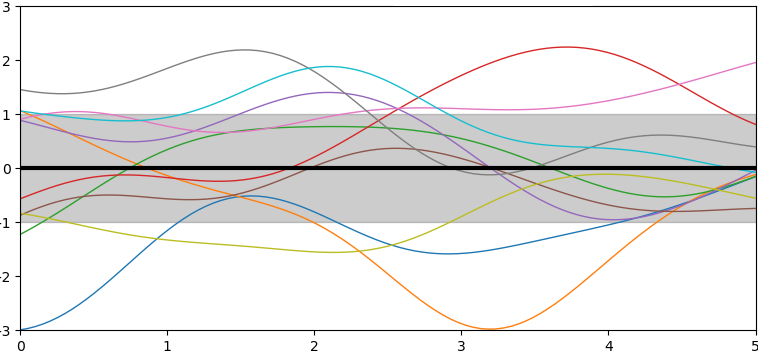
\includegraphics[width=0.45\textwidth]{RBF_prior}
	\label{fig:RBF_prior}}
	\hfill % no empty line here to avoid staring a new paragraph (figures will be vertically aligned)
	\subfigure
	[RBF kernel posterior ($length scale = 0.279$)]
	{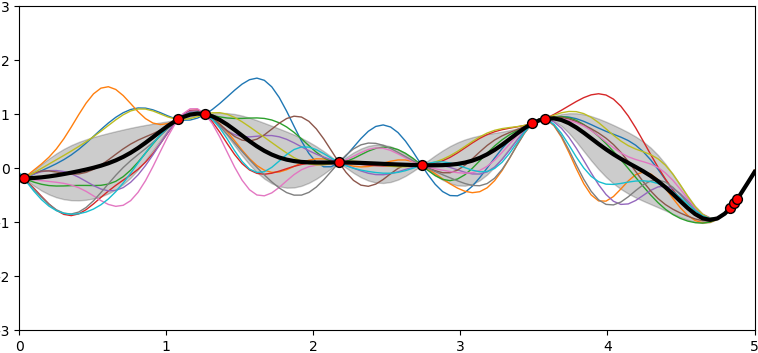
\includegraphics[width=0.45\textwidth]{RBF_posterior}
	\label{fig:RBF_posterior}}
	\caption[Prior and posterior of RBF kernel]
		{\hspace{-0.18cm}\footnotemark\ 
		Prior and posterior distributions of an RBF kernel with mean zero, resulted in a Gaussian process $\mathcal{GP}\left( 0 (\vec{x}), \Sigma(\vec{x}) \right)$.
		Each color line stands for a drawing (prediction) from the prior and posterior distributions, and the thicker black line shows the overall mean of the distributions.
		The red circles are the known data points on which the kernel was optimized to fit, and the gray areas mark the \SI{95}{\percent} confident intervals above and below the overall mean.
		The length scale parameter (in parentheses) determines the length of the \enquote{wiggles} of the functions}
	\label{fig:RBF_prior_posterior}
\end{figure}
\footnotetext{adapted from \url{https://scikit-learn.org/stable/_images/sphx_glr_plot_gpr_prior_posterior_001.png}}

As also motivated in \cref{subsec:limitations_of_did,subsec:temporal_analysis}, artificially splitting interactions into a fixed, pre-determined number of parts to measure accommodation results in a partial view on the process.
To avoid that, some interpolation method is required, with the goal of generating a more general behavior based on the observed productions.
This allows analysis on continuous series of values instead of point-by-point comparison, where the temporal gaps between data points might be greatly unbalanced.
One way of achieving that, using \ac{loess}, is shown in \cref{fig:hds_dds_time_pitch}.
A more evolve approach is presented here, where a speaker's vocal behavior is described as a distribution of functions that match the accumulated \textit{evidence} from the speaker's productions.
\todo{integrate these references}
\citet{Galvez2020unifiying}\\ % compare to the rather simplistic (and naive) approach taken here (based on TAMA) -- can refer to some of the specific methods there, specifically that they also use area under curve difference
\citet{Kousidis2008towards}\\ % original TAMA paper. read again, but seems like it's glorified moving average. say that my appraoch actually learns the curve of the speaker and doesn't just interpolate, which allows continuous predictions and more evolve description.
\citet{Kousidis2009monitoring}\\ % another TAMA paper, with an a bit more concrete example

Kriging (or \textit{\acl{gp} regression}) is an interpolation method that gives an optimally fitted and unbiased prediction of intermediate values.
Since this method fits a function distribution over the data, it not only yields mathematically more likely values, but also provides a curve that describes the characteristics of the interpolated curved, as opposed to more naive methods like linear interpolation or smoothing spline.
Another advantage of this method is that it offers a \textit{distribution over functions} rather than specific values.
Therefore, an infinite number of suitable values can be drawn from one fitted kernel and their likelihood can be evaluated.
Such interpolation is illustrated in \cref{fig:RBF_posterior}, where each line represents a mean regression prediction drawn from the posterior distribution based on the given data points.
To demonstrate this method, it was applied here on the dataset presented in \cref{sec:vacc}.
For simplicity, only the interactions in solo condition were used.
The \ac{gp} prediction for each speaker can be described by
%
\begin{equation}
	\label{eq:gp_function_prediction}
	f_*(\vec{x}) = \mathcal{GP}(\mu_{\vec{x}}, \Sigma_*),
\end{equation}
\eqname{Function predicted using a fitted Gaussian process}\noindent
%
where $\mu_{conv}$ is the mean feature value of a single speaker and $\Sigma_*$ is the fitted additive covariance function described in \cref{subsec:covariance_functions}.
It is important to note that the mean is not zeroed (as usually done in \ac{gp} regression) to maintain the original input values for the subsequent steps.
The kernel was initialized with the priors $C = 1$, $lengthscale = 1$, and no assumptions regarding noise level.
The search boundaries for the RBF and noise components were $1 < lengthscale < 100$ and $\num{1e-4} < \xi < 10$, respectively, with a maximum of six optimization iterations. % the initial one plus five allowed restarts (n_restarts_optimizer parameter in code)
% \xi is here the sign for noise
\todo[inline]{make sure these numbers are up to date}
\todo[inline]{write about how datapoints where selected from each turn to represent points of change}
With the fitted kernel, a continuous prediction can be made for each speaker over the entire conversation time span.
\Cref{fig:gp_vacc} shows an example of \ac{gp} predictions for one of the conversations. % 20171121A_Calendar_01 was used
%
\begin{figure}[t]
	\centering
	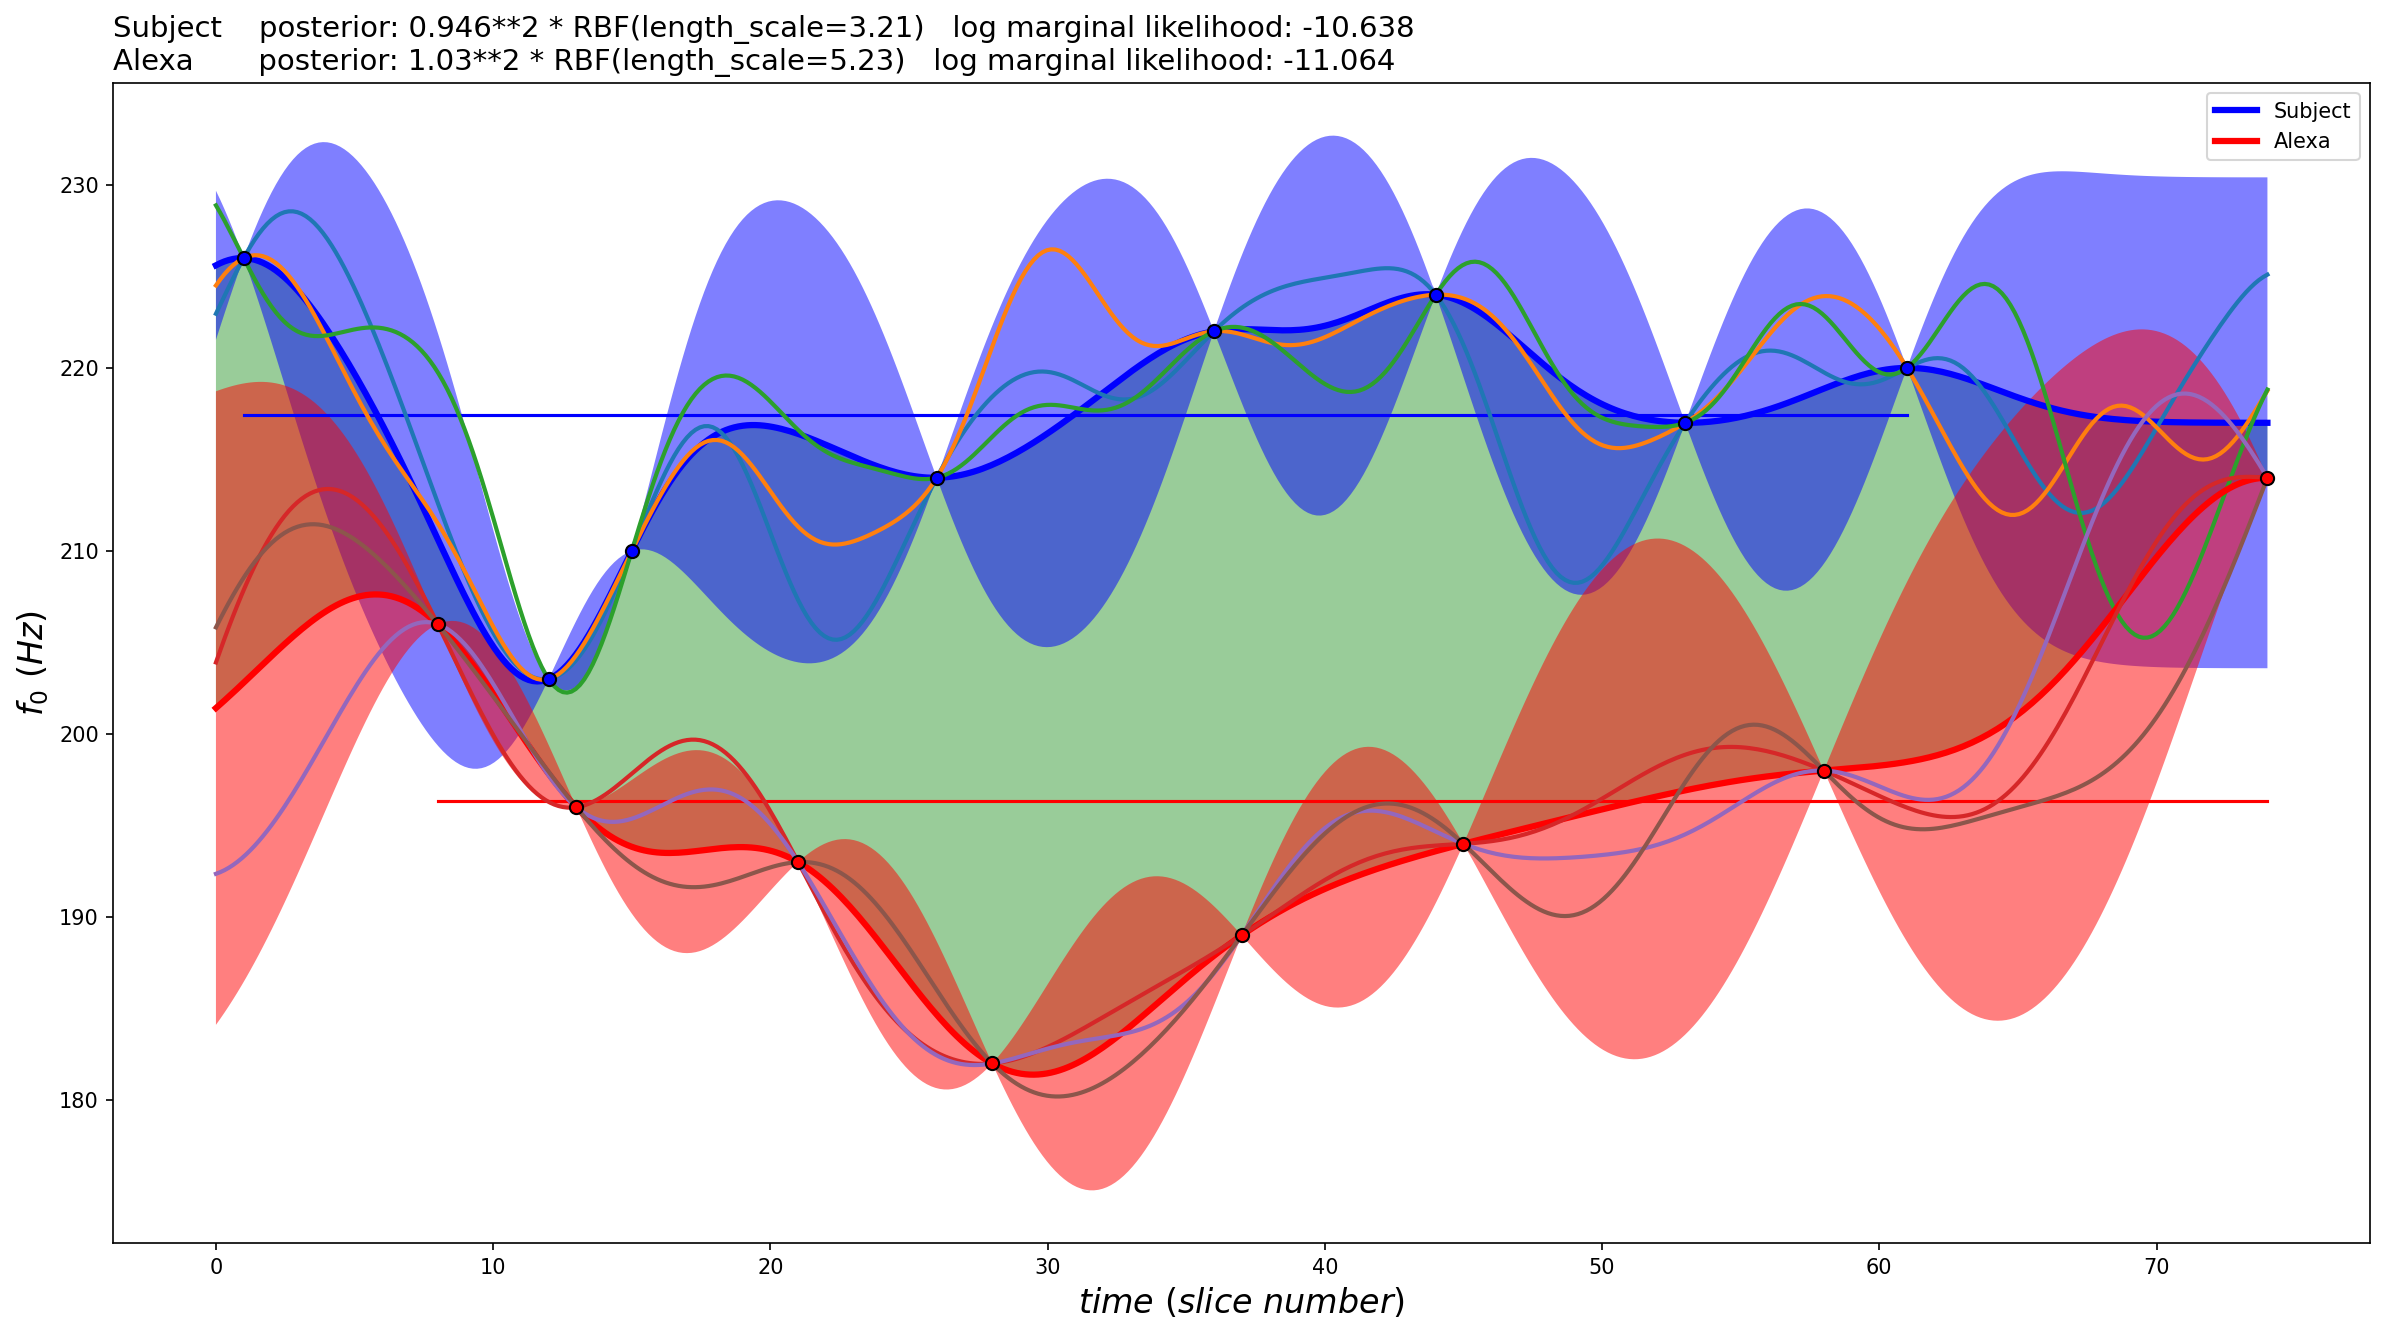
\includegraphics[width=\textwidth]{GP_VACC_with_draws}
	\caption[Gaussian process regression on a conversation with Alexa]
		{Gaussian process regression for an interaction of a subject with Alexa.
		 The thick blue and red lines show the predictions' mean.
		 The additional lines around the means are randomly drawn functions from the fitted kernel representing potential variational output.
		 The colored areas around the means lines show the \SI{95}{\percent} confident interval for the distributions of the same color.
		 The straight horizontal lines indicate the overall mean of each speaker's productions.
		 The posterior parameters and the log marginal likelihoods of the fitted distributions are stated at the top.}
	\label{fig:gp_vacc}
\end{figure}

\section{Marking degrees of change}
\label{sec:measuring_changes}

Once a regression line is drawn for each speaker from their respective distributions, the differences between the speakers' productions can be measured.
Furthermore, due to the higher temporal resolution, more fine-grained degrees of change over time can be calculated as well.
The differences are calculated by the subtracting the trapped areas between the two regression lines (see \cref{fig:gp_vacc})
%
\begin{equation}
	f_{diff} \equiv\Delta\vec{x}_* =
	\int_{\vec{x}_i}^{\vec{x}_{j}}\mu_{f_*subject} -
	\int_{\vec{x}_i}^{\vec{x}_{j}}\mu_{f_*alexa}
\end{equation}
%
and the directional derivatives of the resulted delta line to measure the degree of change
%
\begin{equation}
	\nabla\Delta\vec{x}_*' = \frac{d}{dx}f_{diff}
\end{equation}
%
along the difference line.
\Cref{fig:diff_and_derivatives} demonstrates this on the same conversation from \cref{fig:gp_vacc} using the mean predictions of each speaker.
%
\begin{figure}[t]
	\centering
	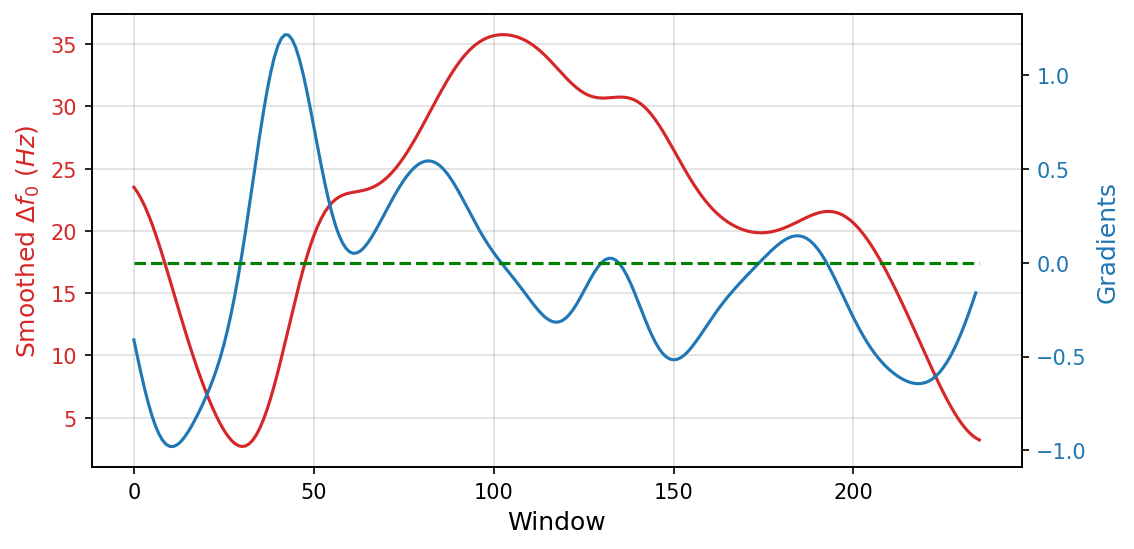
\includegraphics[width=\textwidth]{diff_and_derivatives}
	\caption[Continuous integral differences and derivatives in a \acl{hci}]
		{Continuous integral differences (red line) and their corresponding derivatives (blue line) of speakers' productions in a conversation.
		 The dashed green line shows the zero-gradient, , i.e., no change, threshold.}
	\label{fig:diff_and_derivatives}
\end{figure}
%
For building a generative model as described in \cref{sec:accommodation_as_a_lm,sec:clustering_and_incremental_generation}, the changes must be marked with pre-defined labels.
To that end, the derivative values were translated into a continuum of change ranging from \textit{divergence} to \textit{convergence}.
Based on this continuum, a discrete scale can be defined.
The more categories this discrete scale offers, the more specific the behavior descriptions can be.
\Cref{fig:cont_disc_scales} shows this process for a discrete scale of three categories: divergence, no (major) change, and convergence.
%
\begin{figure}[t]
	\centering
	\subfigure[Continuous scale]
		{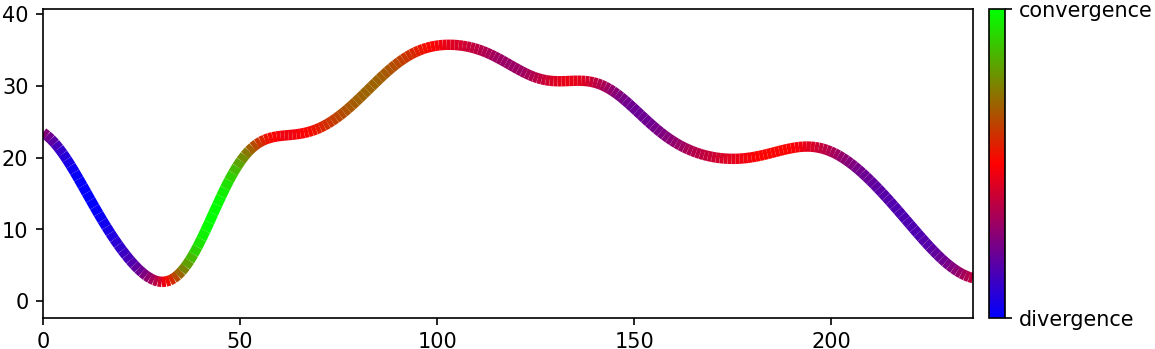
\includegraphics[width=0.47\textwidth]{cont_scale}
	\label{fig:continuous_scale}}
	\hfill
%	\vspace{-1cm}\hfill\hspace{-1cm}{\hbox{\LARGE $\Longrightarrow$}}\hfill
	\subfigure[Discrete scale]
		{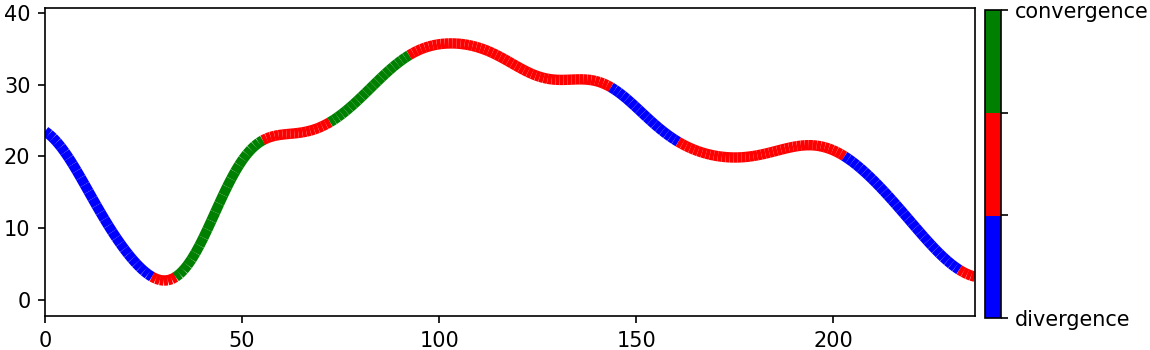
\includegraphics[width=0.47\textwidth]{discrete_scale}
	\label{fig:discrete_scale}}
	\caption[Continuous and discrete scales for labeling degrees of change]
		{Continuous and discrete color-coded scales for labeling degrees of change in a conversation.}
	\label{fig:cont_disc_scales}
\end{figure}
\todo[inline]{more details regarding how the discrete categories are defined}

\section{Accommodation as a language model} % Accommodation as an n-gram model
\label{sec:accommodation_as_a_lm}

In order to generate accommodation sequences, a model is needed, which can iteratively emits a label based on the seen labels history. 
Predictions of any model based on Markov decision process \citep{Bellman1957markovian} depend only on the current state of the conversation.
This neglects any temporal aspect of the conversation, which is a key component in spoken dialogue and accommodation \putref{cref to one or two places where this point is made}.
One way to overcome this is to extend the transition function of a Markov-based model, so that the previous $n$ states are somehow incorporated into the action $a$ of $P_a(s, s')$.
However, this violates the core idea of a Markov decision process and makes it cumbersome to use.
Therefore, an n-gram model is proposed here, which incorporates a portion of a sequence's history (or \emph{context}) into the decision making, without losing the Markov property.
The estimation of the element $e$ at position $i$ is therefore calculated by the probability term $P(e_i \mid e_{i-(n-1)},\ \ldots\ , e_{i-1})$.
N-gram models are traditionally used for describing sequences of some linguistic units, e.g., words in a language model \citep[e.g.,][]{Niesler1996variable}, and are used in applications like machine translation \citep{Marino2006ngram} and proteins identification \citep{Xu2015identification}.
The n-grams model here describes sequences of \emph{accommodation levels} across interactions.
These levels are represented by discretized values that are based on the degrees of change acquired in \cref{sec:measuring_changes}.
After computing the n-grams probabilities of the level, this model can be used for generating new sequences.
The resolution and variability of the model can be controlled by changing the n-grams' $n$ and the number of levels used to distinguish between the different accommodation levels.

\subsection{Dimensionality reduction and symbolic representation}
\label{subsec:dim_reduction_and_symbolic_rep}

The gradient time series extraction process described in \cref{sec:measuring_changes} (and see \cref{fig:diff_and_derivatives}) is greatly high dimensional, even for short interactions.
While this representation is useful for obtaining a fine-grained overview of the data, it is not practical for various analysis techniques that do not benefit (or are not designed to handle) such high dimensional data.
For instance, clustering algorithms, which need to iteratively compare between all points in a collection, scale better with lower dimensionality.
The dimensionality of the data in question here is reduced using \acf{paa} \citep{Keogh2001dimensionality}, which is a common dimensionality reduction technique for time series.
Each element $\vec{x}_i$ of the reduced vector is calculated by
%
\begin{equation}
	\label{eq:paa}
	\vec{x}_i = \frac{N}{n} \sum_{j=\frac{n}{N}(i-1)+1}^{i(\frac{n}{N})} S_j,
\end{equation}
\eqname{\Acl{paa} dimensionality reduction}\noindent
%
where $n$ is the dimensionality of the original times series, $1 \leq N \leq n$ is the dimensionality of the output vector, and $S_j$ is the $j$\textsuperscript{th} element of the original time series.
\Ac{paa} is suitable here, as the goal is to obtain vectors with fewer dimensions that still faithfully represent the data, and not, e.g., decompositions of the original data \citep[cf.\ method survey in][pp.\ 271-275]{Keogh2001dimensionality}.
As the goal here is to compare \emph{trends in change} within and across conversations rather than their absolute values, all gradient time series where z-normalized before applying the \ac{paa}.
Ultimately, \ac{paa} provides \textbf{continuous numeric values} that represent the overall shape of the original time series.
\todo{if eventually relevant, say that this normalization is reversed again when actual values are generated}
\Cref{fig:paa} illustrates \ac{paa} on the gradients of one of the interactions.

\begin{figure}[t]
	% 20171130A_Quiz_01 was used for these figures
	\centering
	\subfigure[\acs{paa} based on the original time seires.
			   The blue continuous line shows the original time series representing the mutual change gradients in a conversation, which was extracted as described in \cref{sec:measuring_changes}.
			   The organe circles show the \acs{paa} points created based on the continuous lines.
			   The dashed orange line is the linear interpolation between the \acs{paa} points.
			   Note that this lines is for illustration only and is not taken into account for any \acs{paa}-related analysis.]
		{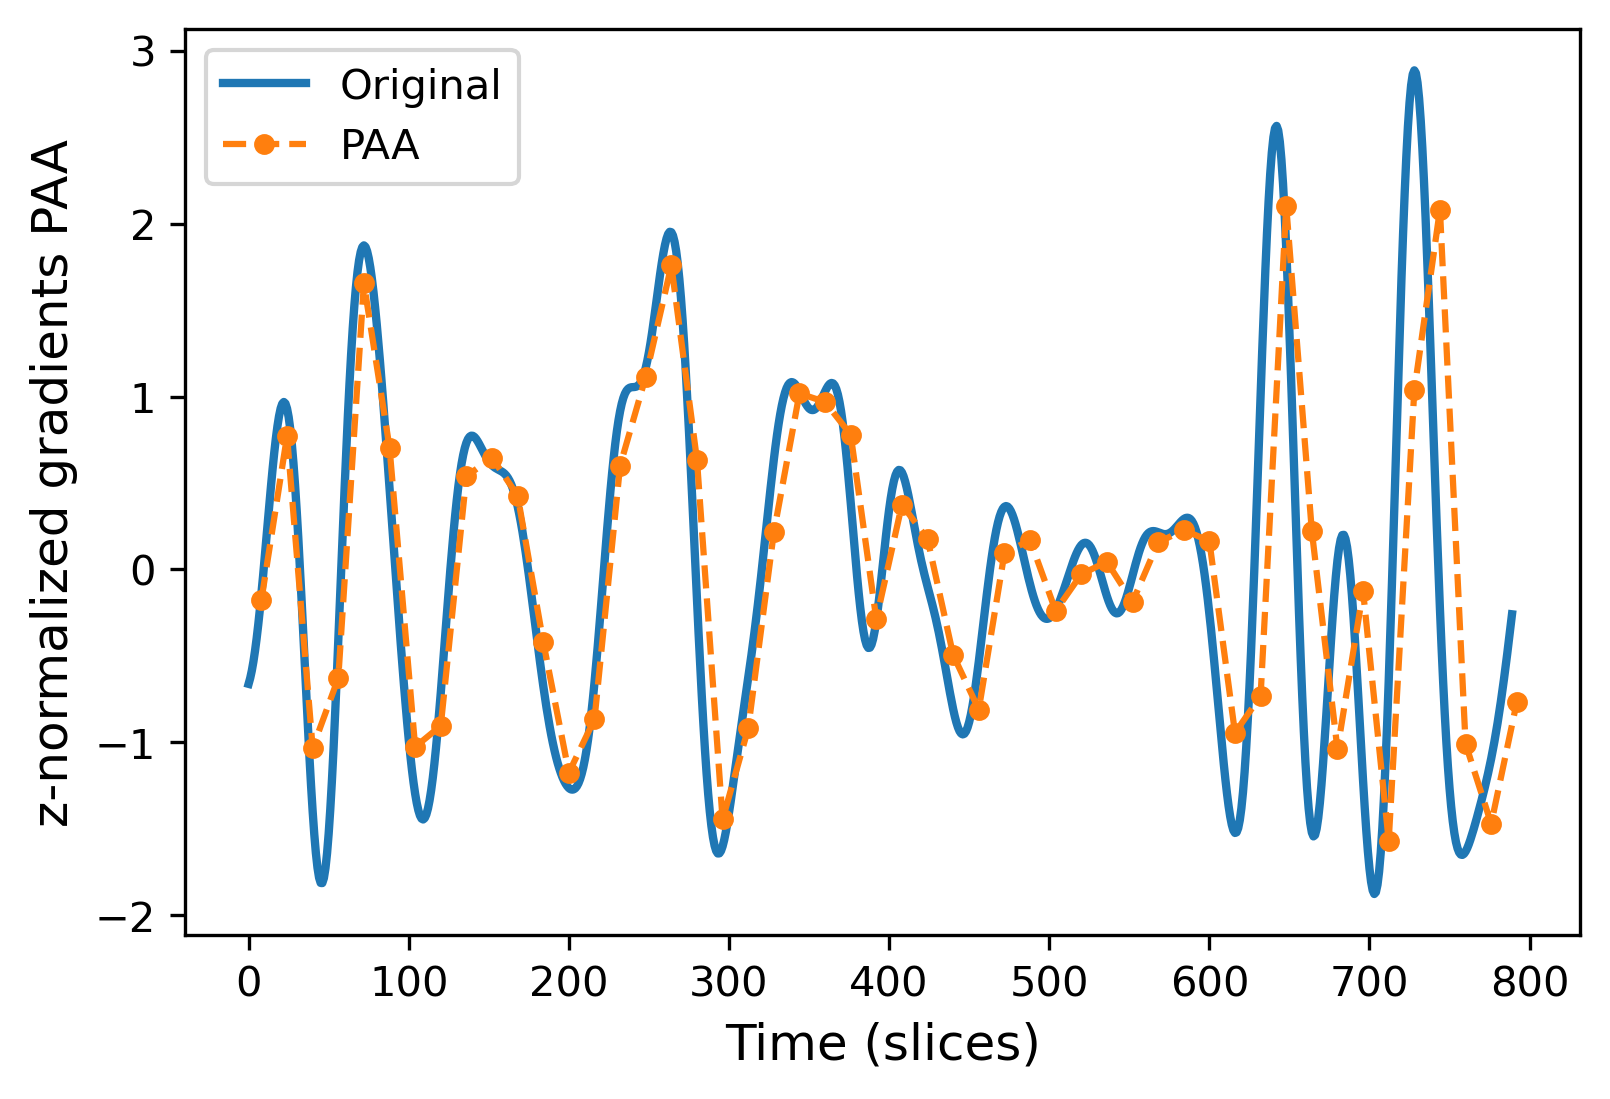
\includegraphics[width=0.47\textwidth]{PAA}
	\label{fig:paa}}
	\hfill
	\subfigure[\acs{sax} based on the \ac{paa} values.
			   The blue circles are the \acs{paa} points from \cref{fig:paa}.
			   The blue line visualizes the linearly interpolated trend of these points.
			   The horizontal green dashed lines show the margins of the five bins that split the points discrete categories derived from a normal distribution.
			   The organe labels (\enquote*{d+}, \enquote*{d}, \enquote*{n}, \enquote*{c}, and \enquote*{c+}) mark the classification of each point based on the bin it falls into.]
		{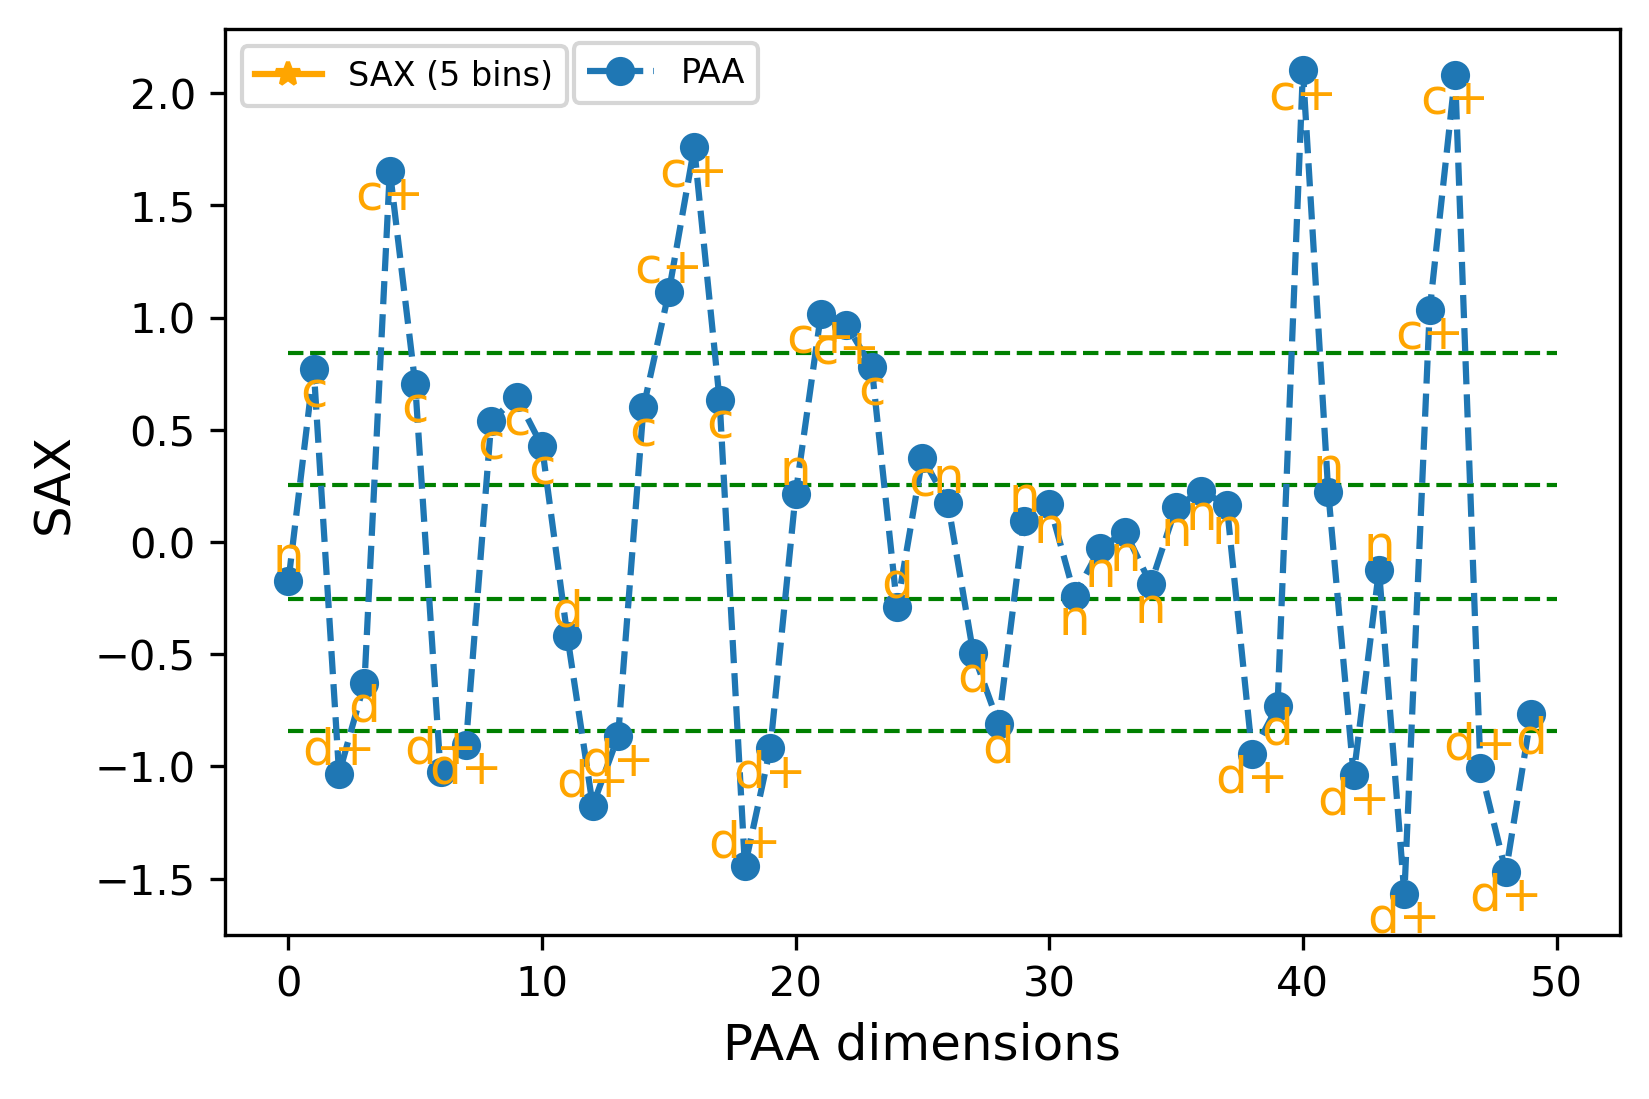
\includegraphics[width=0.47\textwidth]{SAX}
	\label{fig:sax}}
	\caption[\Acl{paa} and \acl{sax} for the time series representation of mutual change in a conversation]
		{\Ac{paa} and \ac{sax} for the time series representation of mutual change in a conversation.}
	\label{fig:paa_and_sax}
\end{figure}

\Ac{paa} is suitable for analyses of continuous numeric values.
However, discrete values are required for symbolic sequence-based processing, such as calculating probabilities of n-grams.
For converting the continuous \ac{paa} values, the \acf{sax} \citep{Lin2007experiencing} method was used.
\Ac{sax} assigns a string label to each of the pre-defined bins.
This is an advantage of \ac{sax}, as these labels provide a more meaningful and intuitive representation for humans.
As explained, e.g., by \citet{Apostolico2003monotony}, it is preferable to use a discretization technique that outputs a symbol set with equiprobability\footnote{It can be claimed that realistically equiprobability does not hold for the symbols in this kind of data.
While that may be true to some extent, neither the pre-processing nor the dimensionality reduction steps held any assumptions regarding the values in each \ac{paa} sequence.
Moreover, the data was z-normalized to avoid any bias stemming from specific numeric values.
For these reason, together with the fact that the participants were, in practice, free to speak in whatever way they wanted, equiprobability can be assumed in this analysis.
See \cref{subsec:word_extraction_and_seq_prob} for more information regarding the distribution of extracted symbol sequences}.
To that end, the \ac{sax} discretization was done using bins based on the normal distribution:
% this is defined by the method="normal" parameter in the SAX function (or `strategy` parameter internally)
\todo{can express the binning as a formula?}
Five categories (bins) are used here for categorizing degrees of change, labeled \enquote*{d+} for \emph{strong divergence}, \enquote*{d} for \emph{divergence}, \enquote*{n} for \emph{no (major) change}, \enquote*{c} for \emph{convergence}, and \enquote*{c+} for \emph{strong convergence}.
This number was found to adequately describe types of accommodation;
Three categories resulted in too unspecified sequences where all degrees of convergence or divergence are labeled similarly (as in \cref{fig:discrete_scale}), and seven or more categories did not add a substantial added value and often yielded in sparse sequences.
The motivation for choosing an odd number of categories is to have a \enquote{no-change} category.
However, an even number can be used as well, forcing each value to stand for either convergence or divergence while ignoring zero values.
Note that the term \emph{synchrony} is avoided here for describing steady distance between the speakers, per the definition introduced in \cref{subsec:variation_types}, which entails additional properties.
Ultimately, \ac{sax} provides \textbf{discrete textual labels}, which are a discretized version of the original time series.
\Cref{fig:sax} shows the \ac{sax} of mutual change time series based on the \ac{paa} points in \cref{fig:paa}.

\subsection{Sequence extraction and probability calculation}
\label{subsec:word_extraction_and_seq_prob}

After applying \ac{sax}, a sequence of accommodation labels was obtained for each corresponding interaction.
The count distribution of the labels was computed to examine their frequency.
As could be expected, the symbol $n$ (standing for no-change) had the highest frequency.
This frequency was about 2.5 times higher than the convergence and divergence labels $c$ and $d$, whose frequency, in turn, was roughly four times higher than the frequency of the strong convergence and strong divergence labels $c+$ and $d+$.
The same process was repeated for combinations of the labels as they appear in the \ac{sax} sequences.
The frequencies could be clearly separated into three groups:
Matching the single-label distribution, repeated $n$ labels were about three times more frequent than the second group, which consisted of most other combinations that included $n$.
Lastly, this group was followed by a longer tail of less frequent sequences, starting from counts three to four times lower, which included the rest of the symbol combinations.
Sequences with many repeated $c+$ or $d+$ labels (i.e., sustained convergence/divergence) always appeared at the end of the tail.
Increasingly smoother instances of the same overall distribution shape were found for all sequence lengths from two up to half the \ac{sax} sequence length (after which such frequencies become not as meaningful).
The percentage of covered n-grams of length $w$ found in the \ac{sax} sequences out of the $5^w$ theoretically possible combinations was exponentially lower the higher $w$ was.

\begin{table}[t]
	\centering
	\caption[Examples of probabilistically generated accommodation level label sequences]
		{Three examples of probabilistically generated accommodation level label sequences.
		 Each sequence consists of eight labels that were generated based on the initial context of the padding symbol $p$.
		 The first line of each example shows the generated symbols as introduced in \cref{subsec:dim_reduction_and_symbolic_rep} and their average variability (value between 0 and 1, higher number means more variability.).
		 The second line lists the scores (probabilities) of each corresponding generated label given the context seen up to that point and the overall probability of generating this entire sequence.
		 The third line lists the perplexity of the trigram ending with the corresponding generated label given the context at the time of the generation.
		 Note that the first two padding labels do not have score values, as they are given as the initial context.
		 Similarly, perplexity can only be calculated once the sequence is longer than the one trigram.}
		 % variability was calculated as the average "deviation", where c and d have value of 0.5, c+ and d+ value of 1, and n value of 0. for Example (c + c+ + n + n + d+ + c + n + n) / 8 = 0.375
	\label{tab:generated_symbol_sequences}
	\begin{tabularx}{\linewidth}{*{10}{c}l@{\hskip 0.1cm}l}
		\toprule
		p    & p    & n    & n    & n    & c    & n    & d    & d    & c    & variability: & \num{0.187}  \\
		---  & ---  & 0.44 & 0.46 & 0.55 & 0.18 & 0.32 & 0.29 & 0.25 & 0.35 & probability: & \num{1.63e-4}\\
		---  & ---  & ---  & 2.22 & 1.99 & 3.16 & 4.16 & 3.27 & 3.67 & 3.35 & perplexity: & \num{3.11}   \\[0.4cm]
		
		p    & p    & n    & d    & d    & c    & c+   & d+   & d+   & c+   & variability: & \num{0.687}  \\
		---  & ---  & 0.44 & 0.17 & 0.25 & 0.35 & 0.13 & 0.25 & 0.34 & 0.19 & probability: & \num{1.37e-5}\\
		---  & ---  & ---  & 3.67 & 4.88 & 3.35 & 4.69 & 5.62 & 3.46 & 3.96 & perplexity: & \num{4.23}   \\[0.4cm]
		
		p    & p    & c    & c+   & n    & n    & d+    & c     & n    & n    & variability: & \num{0.375}  \\
		---  & ---  & 0.30 & 0.25 & 0.25 & 0.16 & 00.04 & 00.20 & 0.22 & 0.41 & probability: & \num{2.16e-6}\\
		---  & ---  & ---  & 3.67 & 4.03 & 5.02 & 12.72 & 11.51 & 4.77 & 3.30 & perplexity: & \num{6.43}   \\
		\bottomrule
	\end{tabularx}
\end{table}

N-grams of $n = 3$, i.e., trigrams, were used here for computing the probabilities.
The size of the n-gram determines the amount of previously acquired evidence that can be use to calculate a subsequent value.
This fulfills the same role as the \emph{pool size} parameter of the computational model (see \cref{sec:parameters}).
In both cases, the goal is to account for the temporal evolution of the conversation for deciding on its continuation.
To account for conversation-initial sequences, the beginning of each symbol sequence was padded.
The end of the sequence was not padded, since, unlike a traditional language model, the generative model here lets the user decide on the end of the interaction (see \cref{sec:clustering_and_incremental_generation}).
This summed up to a collection of \num{2700} trigrams, which comprised 143 out of the $5^3$ level combinations~1~$\times$~5~two-padding combinations~+~5~$\times$~5~one-padding combinations~$= 155$~possible symbol combinations (\SI{92}{\percent}).
% 2700 is 54 solo interactions times 50 trigrams for each: the size of SAX used was 50, which gives 48 trigrams. with the 3 trigrams added from padding, it's 50. 50 times 54 = 2700
This shows a great variety in conversation dynamics.
% however, since not all possible combinations are used for training, unseen trigrams can still be seen during generation. we set the vocab to be all possible combinations (plus all initial padded trigrams)
% smoothing??
% probabilities for OOV trigrams?
Based on this n-grams model, sequences of symbols, representing accommodation levels in a conversation, can be probabilistically generated.
For example, the next accommodation level $l$ after two convergence labels is taken from the probability distribution $p(l \mid c,\ c)$.
\Cref{tab:generated_symbol_sequences} shows examples of such probabilistically generated sequences for the eight first accommodation labels of a conversation.
It is worth noticing that the third sequence in the table has lower variability than the second sequence, although its overall probability is lower and its mean perplexity is higher.
That means that, based on this model, interactions with lower variability are not necessarily more likely.
On the other hand, since in most context the probability of label $n$ is relatively high, sequences with many $n$ labels are more likely to appear, on average.

\section{Clustering and incremental variational generation}
\label{sec:clustering_and_incremental_generation}

After defining a unified representation of the mutual changes in interactions over time in \cref{subsec:dim_reduction_and_symbolic_rep}, the question arises whether clusters in these representation can be found to detect general similarities in behavioral patterns.
Two clustering methods are, namely \ac{knn} and hierarchical linkage, each offering a different angle and insights.
The former method is a top-down approach with a pre-defined number of clusters, which offer a more general view on the patterns, and latter a bottom-up approach with no prior assumptions, where more speaker-specific differences can be measured.
It cannot be expected to find completely distinct pattern for each speaker.
However, some separable clusters and general tendencies are expected to emerge, both when inspecting individual speakers and at the collection as a whole.

\todo[inline]{if it's not too much work, see how many subject end up having both their interactions in the same cluster}

\todo[inline]{try look into the clusters to see if they can be defined/described somehow (this is where Alexander's visualization can be used)}

\begin{figure}[t]
	\centering
	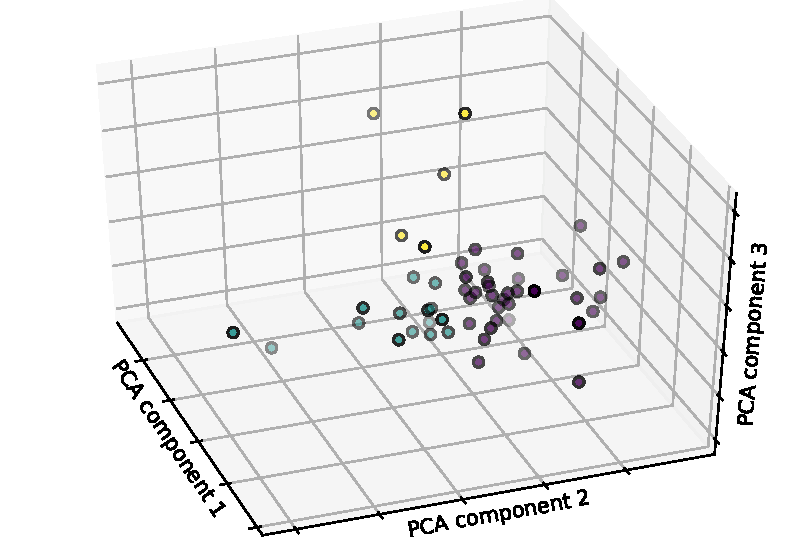
\includegraphics[width=\textwidth]{3d_clustering}
	\caption[3D \ac{knn} clustering of mutual changes \acs{pca} components]
		{\ac{knn} clustering of the first three \ac{pca} components of the interactions' \ac{paa} sequences.
		 Each circle represents one sequence in the three-dimensional space.
		 A circle's color indicates the cluster to which the datapoint belongs.}
		 % elevation is 40 azimuth is 160
	\label{fig:knn_clustering}
\end{figure}

Since the \ac{paa} representations created in \cref{subsec:dim_reduction_and_symbolic_rep} can be arbitrarily long and high dimensional, they are reduced here to their $n$ first \ac{pca} components for the purposes of visualizing their clustering.
The k-nearest neighbors algorithm was used for clustering.
the process was performed for 2, 3, and 5 clusters using the 2 or 3 first \ac{pca}, with the combination of 3 clusters and 3 components performing the best on average.
% on average since kNN is not deterministic and was run multiple times
The result is shown in \cref{fig:knn_clustering}.

\todo{need references for PCA and kNN?}

\begin{landscape}
	\begin{figure}[t]
		\centering
		\hspace*{-4cm}
		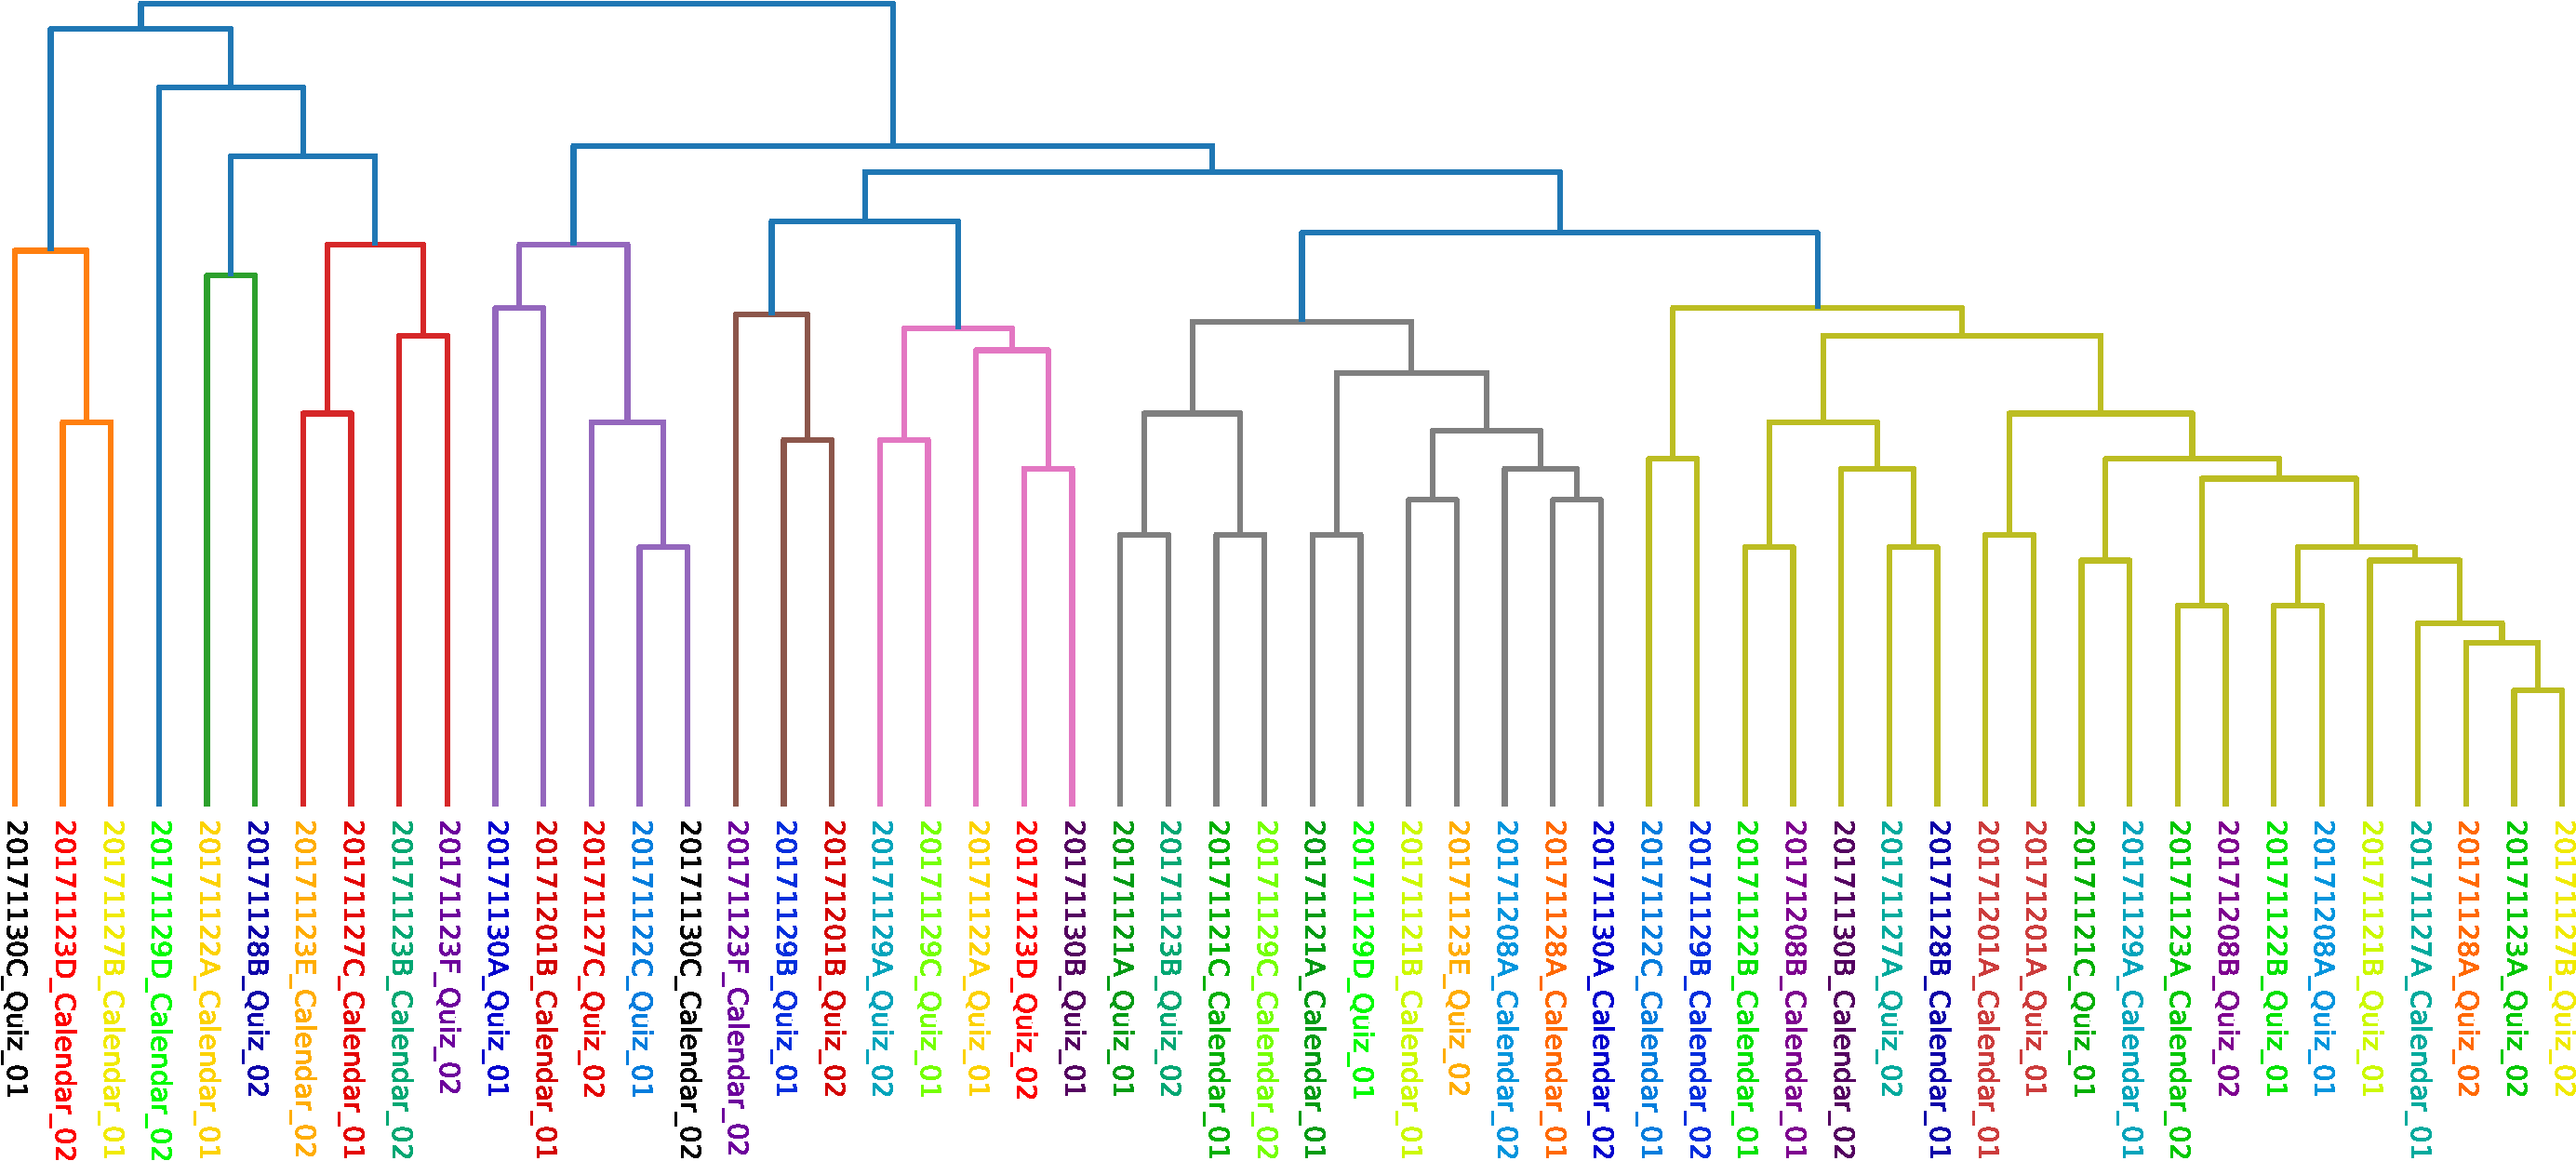
\includegraphics[width=1.7\textwidth]{paa_dist_dendrogram}
		\caption[Dendrogram of time series representation of interactions distances]
			{Dendrogram of the time series \ac{paa} representations of the solo condition interactions based on complete-link distances.
			 Each cluster is represented by a different color of lines.
			 Blue lines connect pairs of clusters that are most similar to each other, and similarly pairs of the closest subsequent sub-cluster and eventually leaves are connect directly to each other.
			 Each leaf represent the interaction indicated by its label.
			 Labels of the same color mark interaction with the same subject (two interactions per subject).
			 The leaf and cluster colors are \emph{not} related.
			 The leaves are order horizontally by their distance from left to right, so that the leaves of interactions that are more similar to each other (both inter- and within-cluster) are positioned closer.
			 For example, the two interactions of subject \emph{20171201A} (12\textsuperscript{th} and 13\textsuperscript{th} leaves from the right) are the closet to each, as they are positioned together and within the same smaller sub-cluster.}
		\label{fig:paa_dist_dendrogram}
	\end{figure}
\end{landscape}

While top-down clustering can uncover general grouping of elements, bottom-up hierarchical clustering can reveal structural relations between them and measure their degrees of similarity.
With numeric values assign to the degrees of changes along an interaction via the the \ac{paa} representations created in \cref{subsec:dim_reduction_and_symbolic_rep}, the distances between the 54 interactions can be measured and compared.
The calculation was done using \emph{complete link} (a.k.a.\ farthest point algorithm) agglomeration technique.
This kind of linkage is supported by the assumption that there are more general behavior patterns beyond the individual differences, as it searches the most dissimilar (and hence principally all) interactions in neighboring clusters and not only the closest one.
This method also allows using the entire \ac{paa} sequences.
\Cref{fig:paa_dist_dendrogram} shows the bottom-up distance clustering based on this linkage. 
Although, unsurprisingly, no definite order emerges, some general trends can be seen regarding the similarity between interactions of the same subject.
As the leaves are ordered horizontally based on their overall similarity, the distances between their positions be utilized to determine each subject's behavior consistency.
The average distance of the population is 16.5, far from the maximal possible average of 27.
% This is the maximal possible average, since this is when each interaction is half of the population away from its pair.
% With the largest possible distance between two leaves being 53, the space can be divided into three bins of 18 (rounded up).
Dividing the space into three equal bins of \enquote{short}, \enquote{medium}, and \enquote{long} distances shows that 16, 10, and 1 interaction(s) fall into these bins, respectively.
Moreover, this distribution has median of 16 and its second tertiles located at 19, far from the \enquote{long distance} bin.
Such skewness in the distribution indicates that interactions of the same speaker tend to be relatively similar in terms of accommodation trends, regardless of any other factor (interaction length, task, order, and other factors used in \cref{chap:speech_variations_in_hhci}).
Notably, the two interactions of one participant, 20171201A, even have the minimal possible distance of 1 between them (12\textsuperscript{th} and 13\textsuperscript{th} leaves in \cref{fig:paa_dist_dendrogram}) and they are located together in the smallest sub-cluster.

\todo[inline]{if the generation based on cluster really works decently, refer to this section when describing variational vocal behavior as one of the levels for accommodative SDS}

\todo[inline]{if it's not too much work, calculate how many subjects are in the same-color cluster}.

\part{Application}
\label{part:application}

\chapter[Accommodation Module for Spoken Dialogue Systems]{Accommodation Module for\\Spoken Dialogue Systems}
\label{chap:convergence_module_for_sdss}

\lettrine{T}{his} chapter introduces a computational model for measuring and applying phonetic convergence as well as a plug-and-use \acs{sds} module that integrates this model.

\pagebreak

\section{Modularization}
\label{sec:modularization}

%\begin{figure}[t]
%	\centering
%	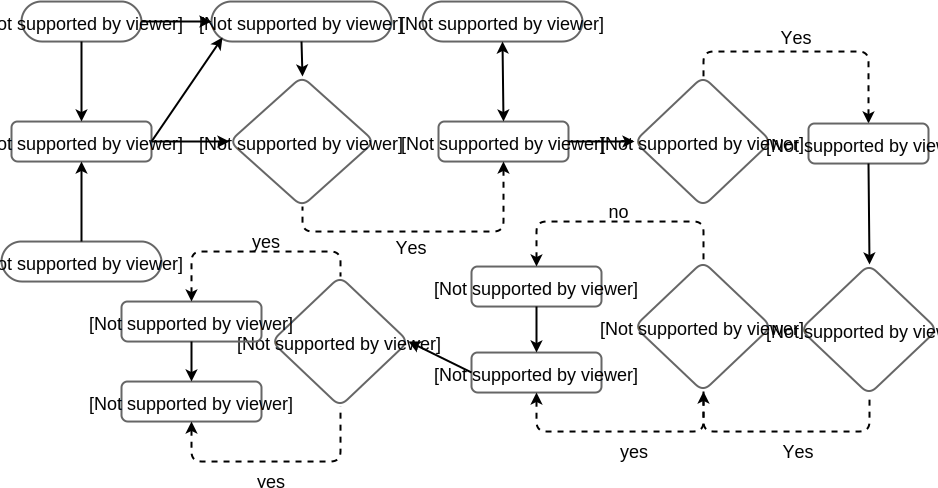
\includegraphics[width=\linewidth]{adaptation_module_pipeline}
%	\caption[Adaptataion pipeline for convergence module] {
%		Overview of the phonetic convergence pipeline used in the computational model. Rectangles
%		represent steps where an action is performed, round rectangles are inputs (either for external resources
%		or from the system), and diamonds stand for decision points. When a decision node does not have a “no”
%		outcome it means that the process is terminated (and therefore no convergence occurs) if the condition
%		is not met. The pipeline can only be successfully completed at the “Set feature’s new value” node.
%		However, if the “Add exemplar” action was performed prior to termination, the exemplar is not removed
%		and will be taken into consideration the next time the pipeline is triggered for the feature with which it is
%		associated. The “Feature definitions” come from the configuration file and can be changed by the user.
%	}
%	\label{fig:adaptation_module_pipeline}
%\end{figure}
\todo{here make an algorithm version of the pipeline (the figure comes later)}

\subsection{Computational model}
\label{subsec:computational_model}

\cref{sec:pipeline_representation}

\todo[inline]{in the intro and in each step add 1-2 sentences about the case of suprasegmental features and say that here the focus is on segmental because they are more complex to track and control and it's one of the novelties here.}

\todo[inline]{make sure that the SemDial paper is referred to.}

\todo[inline]{some intro. say that this is the implementation for the comp model}


The entire computational model is described in \cref{alg:comp_model}.
Further details about the model and all the steps can be found in \citet{Raveh2017Interspeech}.

These will be explained using the following feature definition example, which describes the feature \textit{@\_length}, i.e., length of a segment containing the phoneme schwa (\textipa{[@]}, and cf.\ \cref{subsec:target_features_HCIConv}):
%
\begin{Verbatim}[tabsize=4, commandchars=\\\{\}]
	- \textbf{`@\_length'}:
			\textbf{phoneme}: AX
			\textbf{context}: '.+ AX N'
			\textbf{initial}: 0
			\textbf{minimum}: 0 
			\textbf{maximum}: 80
			\textbf{measure}: duration
			\textbf{calculation}: decaying average
			\textbf{sensitivity}: 0.5
\end{Verbatim}

\subsubsection{Detecting segment exemplars}
\label{subsubsec:detecting segment exemplars}

The first step in the model's pipeline is detecting segments in the user's utterance that can be ascribed to target features defined for the system.
These features are defined in a configuration file that is loaded by the model.
For that, an \ac{asr} engine that emits phoneme times is required.
Here, CMU Sphinx\footnote{\url{https://cmusphinx.github.io/}} was used, with extended functionality to support emission of phoneme-level information.
This additional functionality was build specifically for this purpose (and as part of the system described in \cref{chap:web-based_responsive_spoken_dialogue_system}), with emphasis on phoneme-boundary accuracy.
Each feature is represented by a YAML\footnote{YAML Ain't Markup Language \url{http://yaml.org/}} dictionary entry, which in turn contains a dictionary itself, where each key-value pair refer to a property of that feature that is relevant for the system's accommodation.
Concretely, the phoneme \textipa{[@]} is labeled as \textit{AX} in the German CMU phonemeset, which was the phonemeset used in CMU Sphinx.
This is defined by the \texttt{phoneme} key in the feature definition above.
The key \texttt{measure} sets the measure by which this feature is evaluated; here, its duration.
Other measures are \enquote{formants} (for vowel quality), \enquote{category} (for categorical differences), and more.
This feature's initial value in the system's representation for it is set by the key \texttt{initial}.
This step is performed for each feature separately against each recognized phoneme (see \cref{alg:comp_model}).
Phonemes not ascribed to any defined feature are ignore.

\subsubsection{Filtering exemplars}
\label{subsubsec:filtering_exemplars}

Seeing that segmental features are detected merely based on a phoneme in which they \emph{may} occur, additional filtering is required to retain only those instances where they do.
For example, the target feature \textit{@\_length} introduced in \cref{subsubsec:detecting segment exemplars} aims to capture the German phonological process of elision or epenthesis of \textipa{@} in word-final \textit{<-en>}.
%
%(simplified version adapted from \citet[pp.\,142--143]{Benware1986phonetics}):
%
%\begin{equation}
%	\label{eq:schwa_elision_rule}
%	\text{\textipa{@}}\longrightarrow \varnothing \diagup
%	\left[\text{-son}\right] \ \_\_ \ \{\text{\#}, \left[\text{+const}\right]\}.
%	\todo{this rule is already defined in \cref{eq:}}
%\end{equation}
%\eqname{Phonological rule: schwa elision}
%
This filtering step comes to add any linguistic considerations related to the phonetic feature in question beside the phoneme itself.
Such considerations can be phonemic context, defined as a phoneme regular expression in the \texttt{context} property, a range of acceptable values, defined by the \texttt{minimum} and \texttt{maximum} keys, or both.
In the case of \textit{@\_length} feature above, only segments appearing in the phonemic context corresponds to a (simplified) context of the phonological rule described in \cref{eq:schwa_elision_rule} are considered, and the feature's representation cannot go above 80 (\si{\milli\second}).
The range's role is to filter out segments with unrealistic values (extremely long segment, unreliable formant values, etc.).
For example, a schwa segment longer than \SI{80}{\milli\second} would sound very unnatural.
Any linguistic knowledge about the feature nature can be reflected in this step.
This is important to make sure that all exemplars taken into account when calculating a new value for the feature (see \cref{subsubsec:calculating_changed_value} are sensible, to prevent unstable behavior of the model due to lack of linguistic knowledge or \ac{asr} errors.

\subsubsection{Storing exemplars}
\label{subsubsec:collecting_exemplars}

The remaining exemplars are stored and can be represented by a matrix, which contains the values of these exemplars.
Since each feature is tracked separately, each matrix $\mathcal{F}$ contains exemplars of a single feature, where each exemplar is a row and each column is a dimension of this feature (e.g., a formant in a vowel quality feature).
For instance, the matrix in
%
\begin{equation}
	\label{eq:feature_matrix}
	\mathcal{F} =
	\begin{bmatrix} 
		v_{11} & v_{12} & \dots  & v_{1m}\\
		v_{21} & v_{22} & \dots  & v_{2m}\\
		\vdots & \vdots & \ddots & \vdots\\
		v_{n1} & v_{n2} & \dots  & v_{nm} 
	\end{bmatrix},
\end{equation}
\eqname{A matrix of a phonetic feature}
\noindent
%
the value $v_{21}$ is the first dimension of the second exemplar of the feature.
The model also defines a \textit{pool size}, which determines how many exemplars are kept for each feature.
This parameter aims to represent short-term mental memory of a feature's pronunciation.
When a new exemplar is stored, it is added to the pool (a memory matrix).
When a feature's pool is reached its maximal size, the oldest exemplar is removed (forgotten) to make space for the newest one.
The exemplars in the pool are later used for calculating the system's change (\cref{subsubsec:calculating_changed_value}).
To calculate the change for each dimension, the feature matrix is first transposed, as in
%
\begin{equation}
	\label{eq:transposed_feature_matrix}
	\textbf{$\mathcal{F}$}^\top =
	\begin{bmatrix} 
		v_{11} & v_{21} & \dots  & v_{n1}\\
		v_{12} & v_{22} & \dots  & v_{n2} \\
		\vdots & \vdots & \ddots & \vdots \\
		v_{1m} & v_{2m} & \dots  & v_{nm} 
	\end{bmatrix},
\end{equation}
\noindent
%
where each row refers to a single \emph{dimension} of the feature, rather than an exemplar.

\subsubsection{Calculating a new value}
\label{subsubsec:calculating_changed_value}

The new value of a feature is calculated based on its exemplar pool.
The way the values in the pool are used to determine the change in the system's representation of the feature is a key aspect of the accommodation process.
A \textit{calculation method} is needed to define this relationship.
Different calculation methods can represent different types of relations and approaches.
For example, it can be simulated that people are more likely to converge to utterances they heard recently than to something they heard before.
A function $g$ is defined so that it maps a vector to a scalar (i.e., one feature dimension) and a function $\mathcal{G}$ which maps a matrix to a vector (the entire feature) by applying $g$ to all the row vectors in $\mathcal{F}$:
%
\begin{equation}
	\label{eq:matrix2vec}
	\mathcal{G}: \mathbb{Q}^{n \times m} \longrightarrow \mathbb{Q}^{m}, \qquad g: \mathbb{Q}^{m} \longrightarrow \mathbb{Q}.
\end{equation}
%
\textit{Decaying average} is used here as a simple way to simulate the effect on the exemplars in the pool.
This measure is similar to normal average, only that in this variation each value contributes exponentially less to the overall average, so that the last (newest) value contributes the most.
Adding such property to the measure gives more weight to new exemplars that were received chronologically closer to the current turn and thus makes the change more strongly influence by the productions closer to the accommodation change.
%Using this measure comes to support the analogy of the exemplar pool to short-term memory, which remembers recent event better than older ones.
Decaying average is defined here as
\begin{equation}
	\label{eq:decaying_average}
	\mu_n = \frac{1}{n}\sum_{i = 2}^{n}(\eta v_i + (1 - \eta )\mu_{i-1}),
\end{equation}
\eqname{Decaying average}
%
with $n$ being the number of elements in a row of the transposed feature matrix (\cref{eq:transposed_feature_matrix}), $v_i$ is the value of the $i$-th element, $\eta$ is the decay rate, and $\mu_{i-1}$ the previously calculated decaying average of the previous elements.
Importantly, any function that maps vectors to scalars can be used to experiment with different methods.
Before setting the updated value as the feature's value, the balance between the feature's current value and its calculated pool value needs to be set.
This is defined by the \texttt{sensitivity} (convergence rate), which determines the sensitivity of this feature (see \cref{sec:parameters}) and is implemented as
%
\begin{equation}
	\Upsilon \equiv \mathcal{C}_u = \rho \upsilon + \left(1 - \rho \right) \mathcal{C}_{u-1},
	\label{eq:convergence_rate}
\end{equation}
\eqname{Sensitivity (convergence rate)}
\noindent
%
where $\Upsilon$ is the new feature value, $\upsilon$ is the calculated pool after applying $\mathcal{G}$, $\mathcal{C}_{u-1}$ is the current value of the feature, and $\rho$ is the convergence rate.
A $\rho$ value of 0 means that no convergence occurs (the current value is retained), a value of 1 will result in complete convergence (the current value is ignored), and $\rho=0.5$ will result in an average between the two.
While the convergence rate is typically a value between 0 and 1, smaller and greater values could be meaningful in some applications to achieve over-divergence or over-convergence, respectively.
As shown in \cref{part:experiments}, peoples' accommodation may vary considerably in \acp{hhi} and \acp{hci} and in different settings.
This parameter can help tuning the system's behavior to achieve the desired behavior in the interaction.
For instance, in a tutoring system for pronunciation training, the desired behavior might be for the system to diverge from users' input when it detects that their pronunciation is wrong.
By reflecting the users' utterance with diverged pronunciation (instead of explicitly pointing out their mistake), the user receives auditory feedback in a more implicit, \enquote{conversational} learning process.

%\begin{equation}
%	\lambda\mathcal{M} = \lambda
%	\begin{pmatrix} 
%		v_{11} & v_{12} & \dots  & v_{n}\\
%		v_{21} & v_{22} & \dots  & v_{2n} \\
%		\vdots & \vdots & \ddots & \vdots \\
%		v_{e1} & v_{e2} & \dots  & v_{en} 
%	\end{pmatrix}
%\end{equation}
%
%\begin{equation}
%	\mathcal{M}_i' = g(\mathcal{M}^{\intercal}_{i \leq m})
%	\label{eq:value_calculation}
%\end{equation}
%\noindent
%where $\mathcal{M}^{\intercal} \in \mathbb{Q}^{m \times n}$ is the transposed exemplar matrix (which comprises vectors of dimension values instead of vectors of exemplar values), $g$ is the chosen calculation method to apply to each vector, $\mathcal{M}' \in \mathbb{Q}^{m \times n}$ is the matrix with the pool values for each dimension of the feature, $i$ is the vector index, and $m$ is the number of rows in $\mathcal{M}^{\intercal}$.

%$\lVert P \rVert $ refers to the Euclidean Norm (or vector's magnitude).

\subsubsection{Setting the new value}
\label{subsubsec:setting_the_new_value}

The final step is to set the newly calculated value as the new value for the feature in the system's representation.
After this step, this new value will be used whenever this feature is used by a system using this model (as shown in \cref{subsec:extended_sds}).
Although this step is fairly straight forward, there is still an important issue to take into consideration here, namely \textit{user imitation}.
After some turns, it might happen that the model calculated a value very close to the user's input and then continues to follow the user's production values, resulting in an imitation of the user.
To avoid imitation, the new value is limited in how close it is allowed to get to the exemplars.
This is done by the global property \texttt{ConvergenceThreshold}, which defines the maximally allowed proximity (in percentage) the new value is allowed to have:
Setting this property to 0.8 (\SI{80}{\percent} means that the new value is not allowed to be changed more than (\SI{80}{\percent} of the difference between the current value and the pool's value (and be set to (\SI{80}{\percent} in case it exceeded this threshold).
Of course, the limitation can also be set to 1 to allow the new value be as similar as \SI{100}{\percent} to the pool's value -- i.e., not limiting it.
The maximal value allowed by the limitation is defined by
%
\begin{equation}
	\label{eq:conv_limit}
	\Lambda = \delta \upsilon \left(1 - \lambda \right),
\end{equation}
\noindent
%
where $\Lambda$ is the maximum convergence value allowed, $\delta$ is set to 1 if the converging values are increasing or $-1$ in case they are decreasing (see \cref{eq:direction}), and $\lambda$ is the convergence limit parameter ($\lambda=0.8$ in the example above).
\noindent
Note that the actual value of this limit depends on the direction in which the convergence occurs, which is defined by
%
\begin{equation}
	\label{eq:direction}
	\delta = 		
	\begin{cases}
		\ \ \ 1 & \text{if } \upsilon \geq \mathcal{C}_t\\
		-1 & \text{otherwise}
	\end{cases}.
\end{equation}
\eqname{Determining accommodation direction}
\noindent
%
That is, if the converging values are increasing, the limit's value will be smaller than the pool value;
and if the values are decreasing toward the pool value, the limit's value will be greater than the pool value.
Ultimately, the final updated value for the feature is determined as follows:
%
\begin{equation}
	\label{eq:new_value}
	\Upsilon = 		
	\begin{cases}
		% newValue - (newValue - (newValue * convergenceThreshold)) * direction
		\upsilon - \Lambda & \text{if }\upsilon - \Upsilon \leq \delta\Lambda\\
		\Upsilon \text{ (unchanged)} & \text{otherwise}
	\end{cases}.
\end{equation}
\eqname{Setting accommodation limit}
\noindent
%
It is important to mention that this limitation not only comes to prevent situations where the model imitates the user's behavior, but is also loyal to empirically observed behaviors in \cref{chap:shadowing_experiment_with_natural_and_synthetic_voices,chap:speech_variations_in_hhci}, where participants typically converged only up to a certain limit.

\addtocounter{myequations}{1}
\begin{algorithm}[h!]
	\caption{Phonetic responsiveness}
	\label{alg:comp_model}
	\eqname{Phonetic responsiveness algorithm}
	\algorithmcaption{Note that \emph{ASRInput} (\cref{line:asrinput}) must not only contain the $n$-best hypotheses, but also their phoneme lists (in chronological order).
	For improving performance, using a single hypothesis is recommended for a small language model and/or when very short sentences are expected.
	Since only the target phonemes are treated (and suprasegmental features where the specific phonemes do not matter), it might not be crucial to get a completely correct \ac{asr} hypothesis if not required for continuing the interaction.
	For example, a \ac{capt} system might rely solely on the realization of specific phonemes, regardless of what the user said or should have said.}
	\DontPrintSemicolon
	\SetKwInOut{Input}{Inputs}
	\SetKwInOut{Output}{Output}
	
	\Input{\underline{$ASRInput$} -- recognized user speech\newline
		   \underline{$targetPhonemes$} -- convergence features\newline}
	\Output{list of feature vectors with converged values\newline}
	
	\ForEach {(phoneme $\in$ ASRInput) $\in$ targetPhonemes}{ \label{line:asrinput}
		$feature \gets$ $phoneme$.associatedFeature\;
		$context \gets feature$.phoneticContext\;
		\uIf {\textbf{not} matches(phoneme, context)}{ \tcp*{filter based on context}
			break\;}
		\uIf {inRange($phoneme$, $allowedRange$)}{ \tcp*{filter based on value range}
			\uIf {poolSize=maxPoolSize}{
				deleteOldestExemplar()\;}
			feature.addExemplar($phoneme$)\;}
		\uElse{
			break\;}
		\uIf {toUpdate $=0$}{
			$method \gets feature$.calculationMethod\;
			$poolValue \gets method$.calculate(pool)\;
			$newValue \gets rate\cdot poolValue + (1-rate)\cdot feature.$value\;
			$threshold \gets convergenceLimit \cdot poolValue$\;
			\uIf {$newValue > threshold$}{ \tcp*{limit convergence}
				$newValue \gets threshold$\;}
			$feature$.value $\gets newValue$\;
			{\em toUpdate $\gets$ updatefrequency}\;}
		\uElse{
			{\em toUpdate $\gets$ toUpdate - 1}\;}}
\end{algorithm}
\todo[inline]{make algorithm more readable, change, variable/method names, etc.}

\subsection{Statistical model}
\label{subsec:statistical_model}

\todo[inline]{this should be a short section to explain how the statistical model can be used together with the comp model to support variational change. emphasize that it is replacing only the update step, while all the rest can remain to enjoy advantages of both models. the comp one can help controlling the input for the stat, e.g., decide how the input to the stat model will be calculated (which is a design choice, as explain in that chapter)}

\section{Integration}
\label{sec:integration}

\subsection{Extended \acl{sds} architecture}
\label{subsec:extended_sds}

The accommodation process can now be utilized, using the implementation described in \Cref{sec:modularization}, and it can now be integrated into a \ac{sds} with a standard architecture (cf.\ \Cref{fig:sds_architecture}) as an separate module.
As this module relies on input from the \ac{asr} module and its output is consumed by the \ac{tts} module, it is inserted as a new, direct link between the two, in additional to their connections to the \ac{nlu} and from the \ac{nlg} modules, respectively.
\Cref{fig:adaptation_module_architecture} shows these connections.
The name of this module, \acf{asp}, doesn't not refer to accommodation, as it could, in principle, be used for other purposes as well.
This may include any processing relying on the user's speech signal, beside transcription.
Since the speech signal is discarded after the \ac{asr} module finishes its processing, not speech-related analysis can be sent as input to the other modules.
Here, this is leveraged by the \ac{tts} module, but such analyses could be useful for also for the \ac{dm} or \ac{nlg} modules, e.g., for matching the response content to the user's mood based on voice characteristics \citep{Braun2016assessing, Rothkrantz2004voice}.
%
\begin{figure}[t]
	\centering
	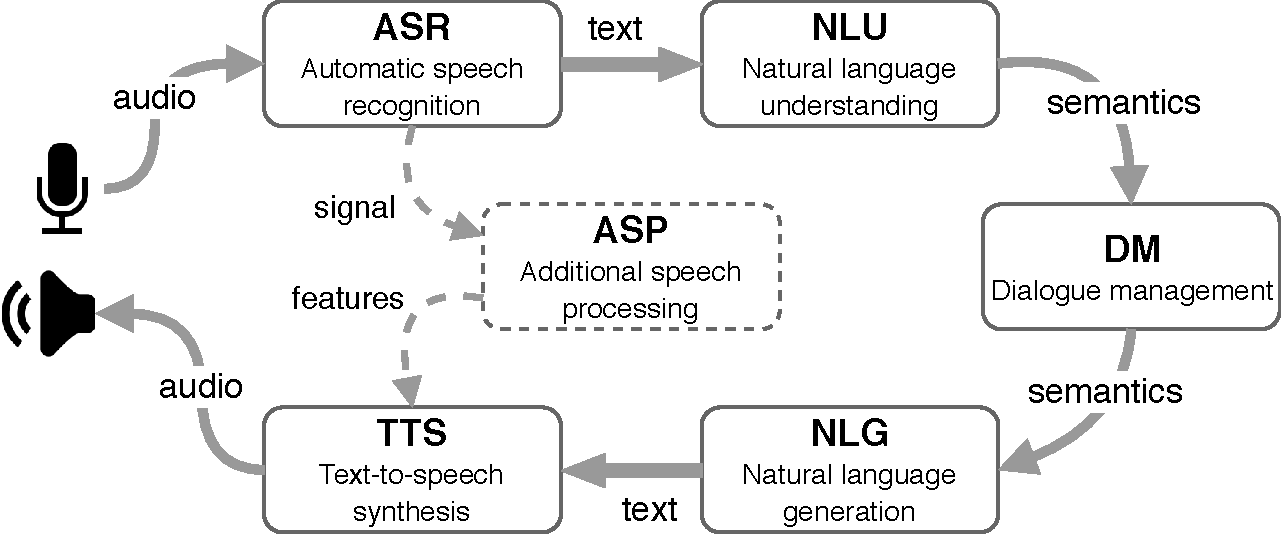
\includegraphics[width=\linewidth]{sds_architecture_ext}
	\caption[Proposed extended architecture of a spoken dialogue system]
		{Suggested architecture for a spoken dialogue system with the phonetic convergence module (cf.\ \cref{fig:sds_architecture}).
		The \acs{asp} module adds a direct link between the \ac{asr} and the \ac{tts} modules to perform additional speech processing used for phonetic accommodation.}
	\label{fig:adaptation_module_architecture}
\end{figure}

\subsection{Speech manipulation}
\label{subsec:speech_manipulation}

\todo[inline]{emphasize that it is real-time}

Although, as explained in \cref{subsec:extended_sds}, the \ac{asp} module is not responsible for the synthesis of the system's speech output, it is important to show that the information it provides could indeed be relevant for speech synthesis.
The examples given here are for segmental features, because real-time manipulation techniques for  them are less common than for supra-segmental features like \ac{f0} and \ac{ar}.
\todo{need reference for this?}
For segmental features, modifications are applied to specific sounds occurring within short time spans, as oppose to supra-segmental features where longer segments (or the entire utterance) are influenced.
The challenge is, therefore, to apply these modifications without distorting the surrounding segments, to maintain the overall smoothness of the synthesized speech.
First, it is required to obtain the time spans to manipulate.
These can be usually provided by the \ac{asr} component of the system (see \cref{subsubsec:detecting segment exemplars}).
Then, the manipulation itself takes place.
What aspect of the signal is modified depends on the target feature.
For instance, the first two formants or an allophone's categorical variant are targeted in the examples below.
Finally, the manipulated segment needs to be connected the rest of the segment while minimizing the distortion.
The way the latter two steps are executed depend on the technique used for the manipulation.
This is demonstrated here by two examples:
One for the \emph{\textipa{[e]} vs.\ \textipa{[E]}} feature, using an approach based on the source-filter theory \citep{Fant1970acoustic}; and one for the \emph{\textipa{[\c{c}]} vs.\ \textipa{[k]}} feature, using a neural approach (both feature are described in \cref{subsec:target_features_HCIConv}).
The main difference between the two approaches is when the manipulation is done.
In the former, the modifications are post-synthesis on an existing audio signal, while in the latter the desired modifications are sent to the synthesizer's as part of its input and can be directly taken into account.
The advantage of this approach is that the resulted signal is more likely to be smoother, as it is not changed after created.
However, the neural approach is prone to overall lesser quality if it is not adequately trained to support changes to the target features.
This would influence not only the time span of the manipulated feature, but the entire generated signal.
Additionally, such \ac{e2e} methods also lack the freedom of directly controlling the manipulation, which may be crucial for achieving the desired final output.
Moreover, for research and evaluation purposes, it is convenient to have both the original and modified signals for comparison and be able to directly control how the changes are applied.
%
\begin{landscape}
	\begin{figure}[t]
		\centering
		\hspace*{-2cm}
		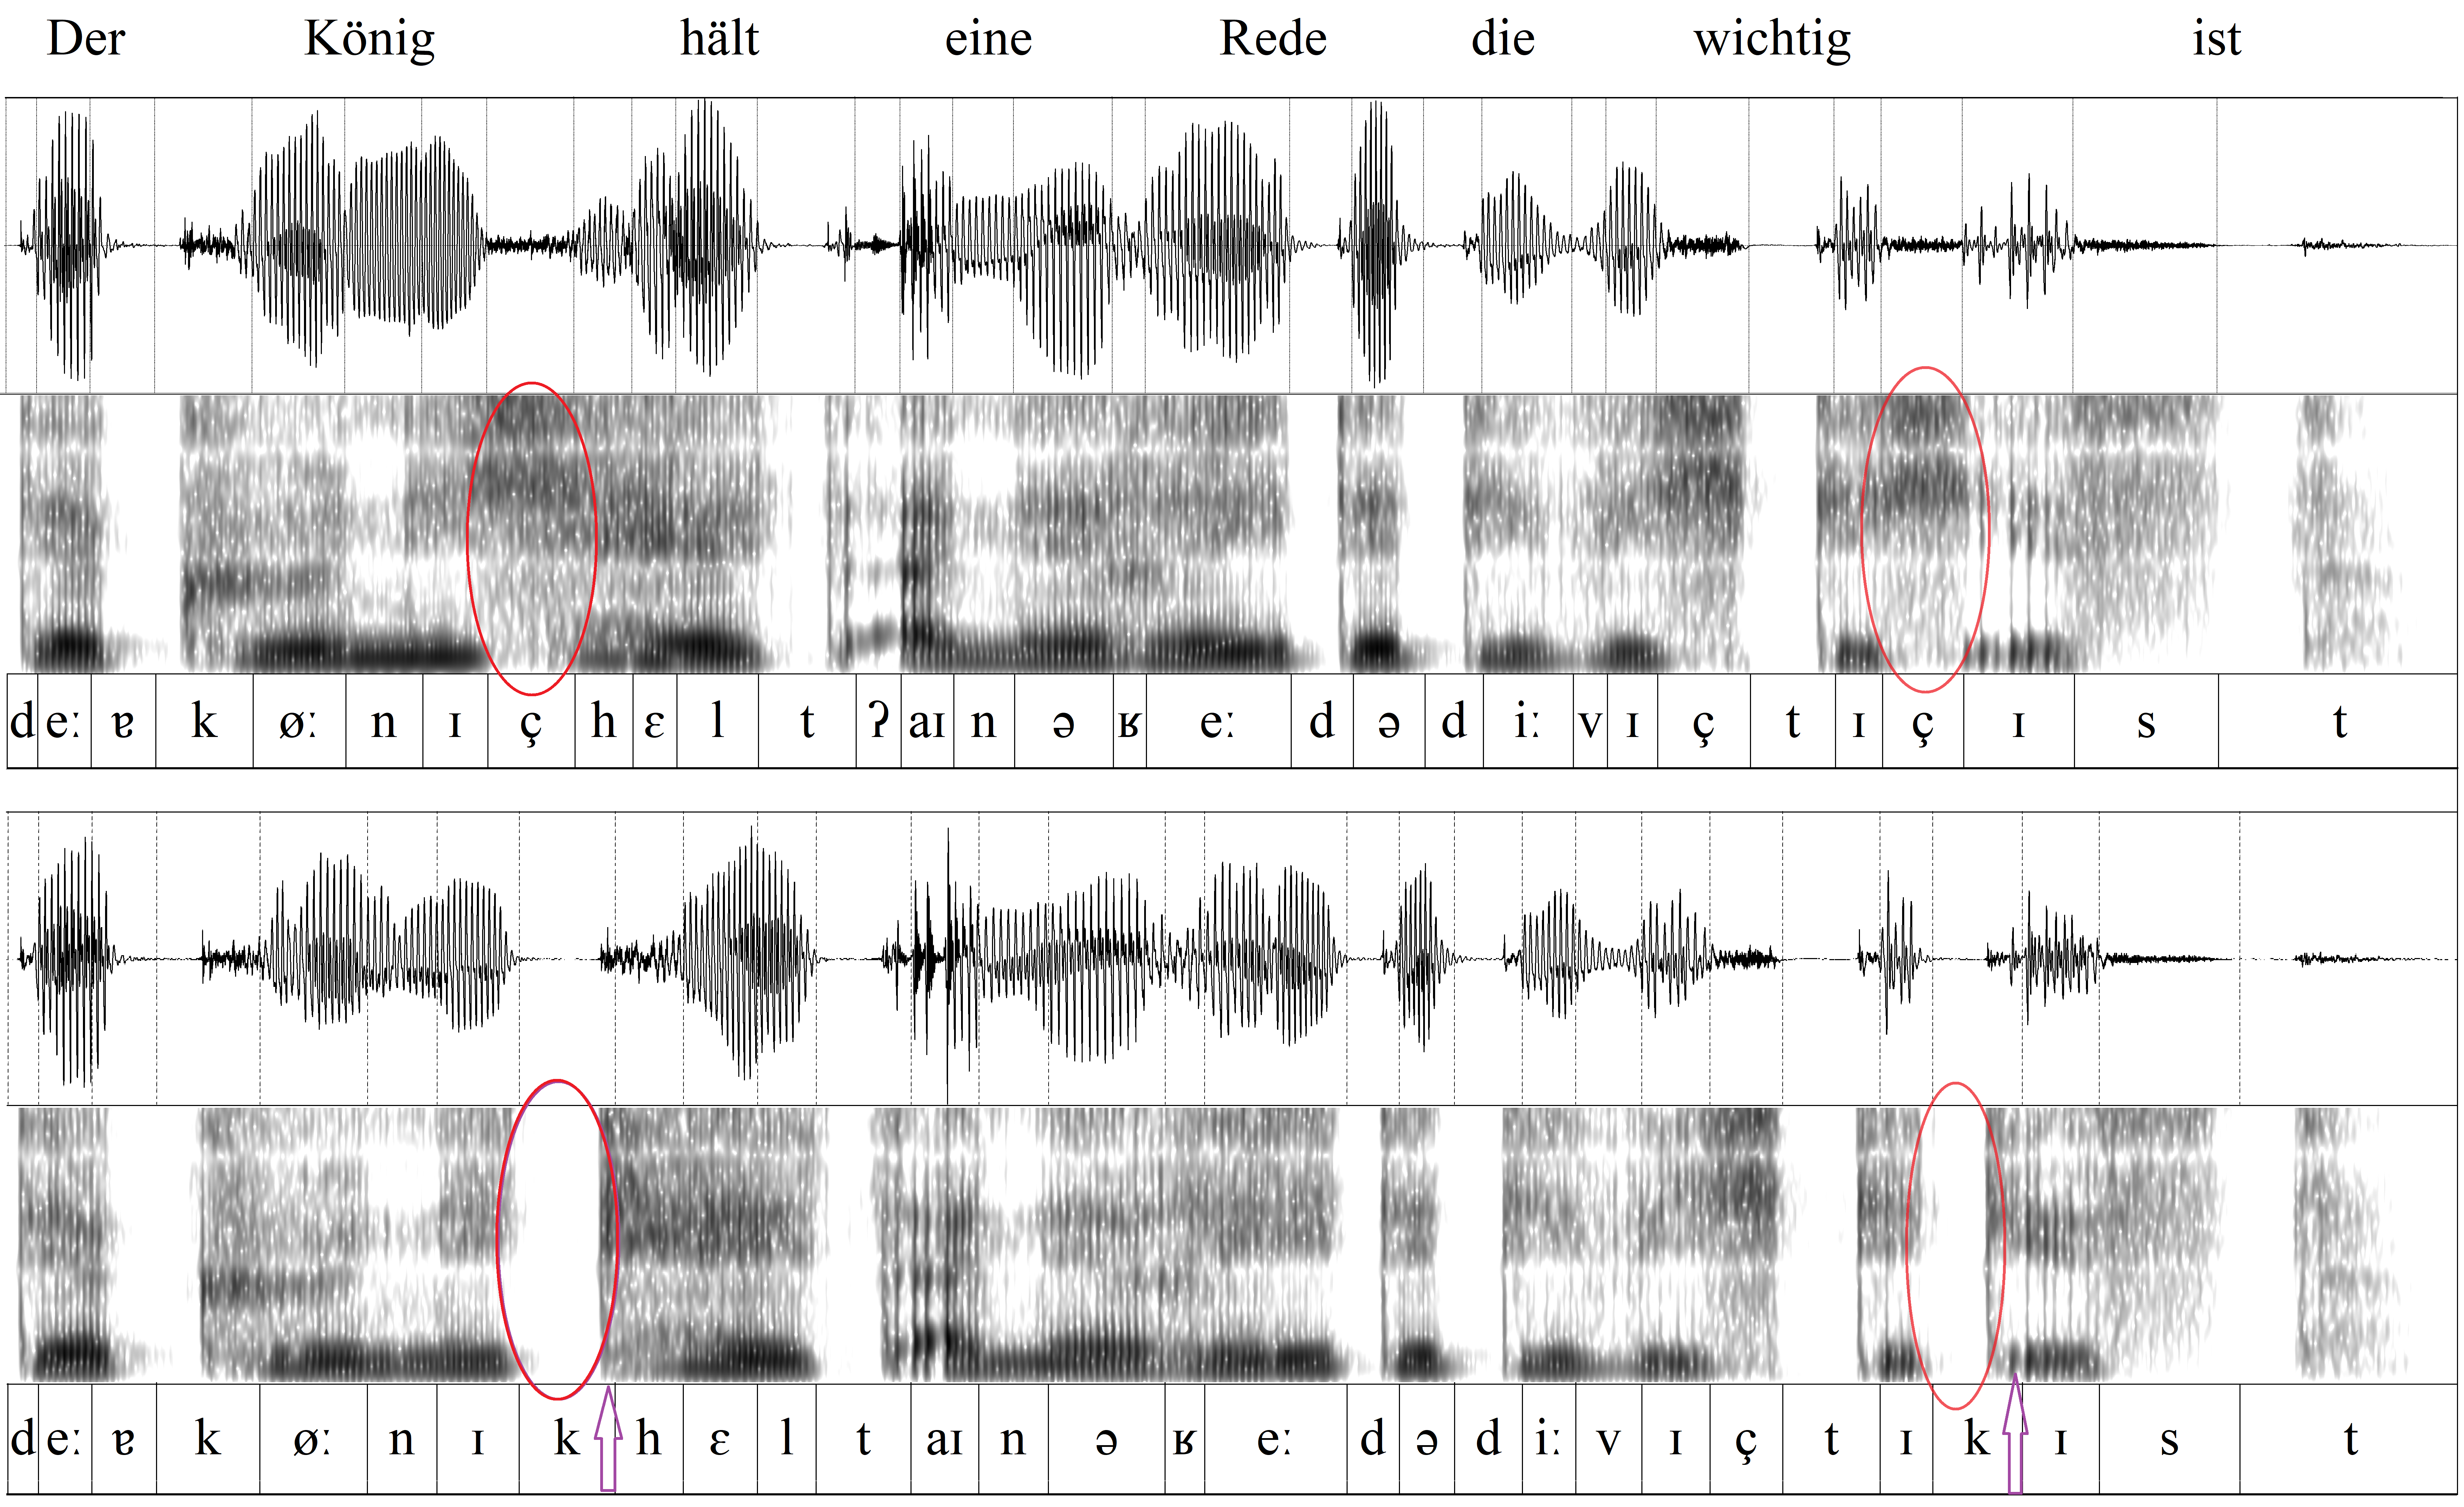
\includegraphics[width=1.5\textwidth]{ic_ik_manipulation}
		\caption[]
			{}
		\label{fig:spectrogram_e_E}
	\end{figure}
\end{landscape}
%

\todo[inline]{explanation of e/E feature}
\missingfigure{spectrogram comparison for e/E feature}

% For each analysis window, Praat applies a Gaussian-like window, and computes the LPC coefficients with the algorithm by Burg, as given by Childers (1978) and Press et al. (1992).

% for the first method, it is also necessary to re-synthesize the audio (overlap-add Moulines & Charpentier (1990), who called it Time-Domain Pitch-Synchronous Overlap-and-Add (TD-PSOLA))

\todo[inline]{explain that e/E is modified on a continuum while c/k is categorical}



The neural-based manipulation is based on Tacotron\footnote{Tacotron2 architecture based on the implementation in the repository \url{https://github.com/NVIDIA/tacotron2}} \citep{Shen2018natural}, which is trained to generate spectral information directly from textual input.
To capture the categorical phoneme variance of the feature \emph{\textipa{[\c{c}]} vs.\ \textipa{[k]}}, the system was trained on \emph{phoneme} input (as oppose to orthographic forms).
For this, the neutral voice subset of the PAVOQUE dataset\footnote{\url{https://github.com/marytts/pavoque-data}} \citep{Steiner2013pavoque} was used ($\sim$\SI{5.8}{\hour} of speech).
The phonetic transcriptions were done automatically based on the transcriptions provided with the dataset and were manually verified and corrected.
\todo{need more details?}
After training, the model was able to generate synthesized speech based on an input of an arbitrary phoneme sequence.
This opens many possibilities, one of them is alternating between \textipa{[\c{c}]} and \textipa{[k]} to express the variation of this feature.
It is important to note that that the other-category variant of a word was not included in any dictionary and was not seen by the model during training.
\Cref{fig:spectrogram_ic_ik}\ldots
%
\begin{landscape}
	\begin{figure}[t]
		\centering
		\hspace*{-2cm}
		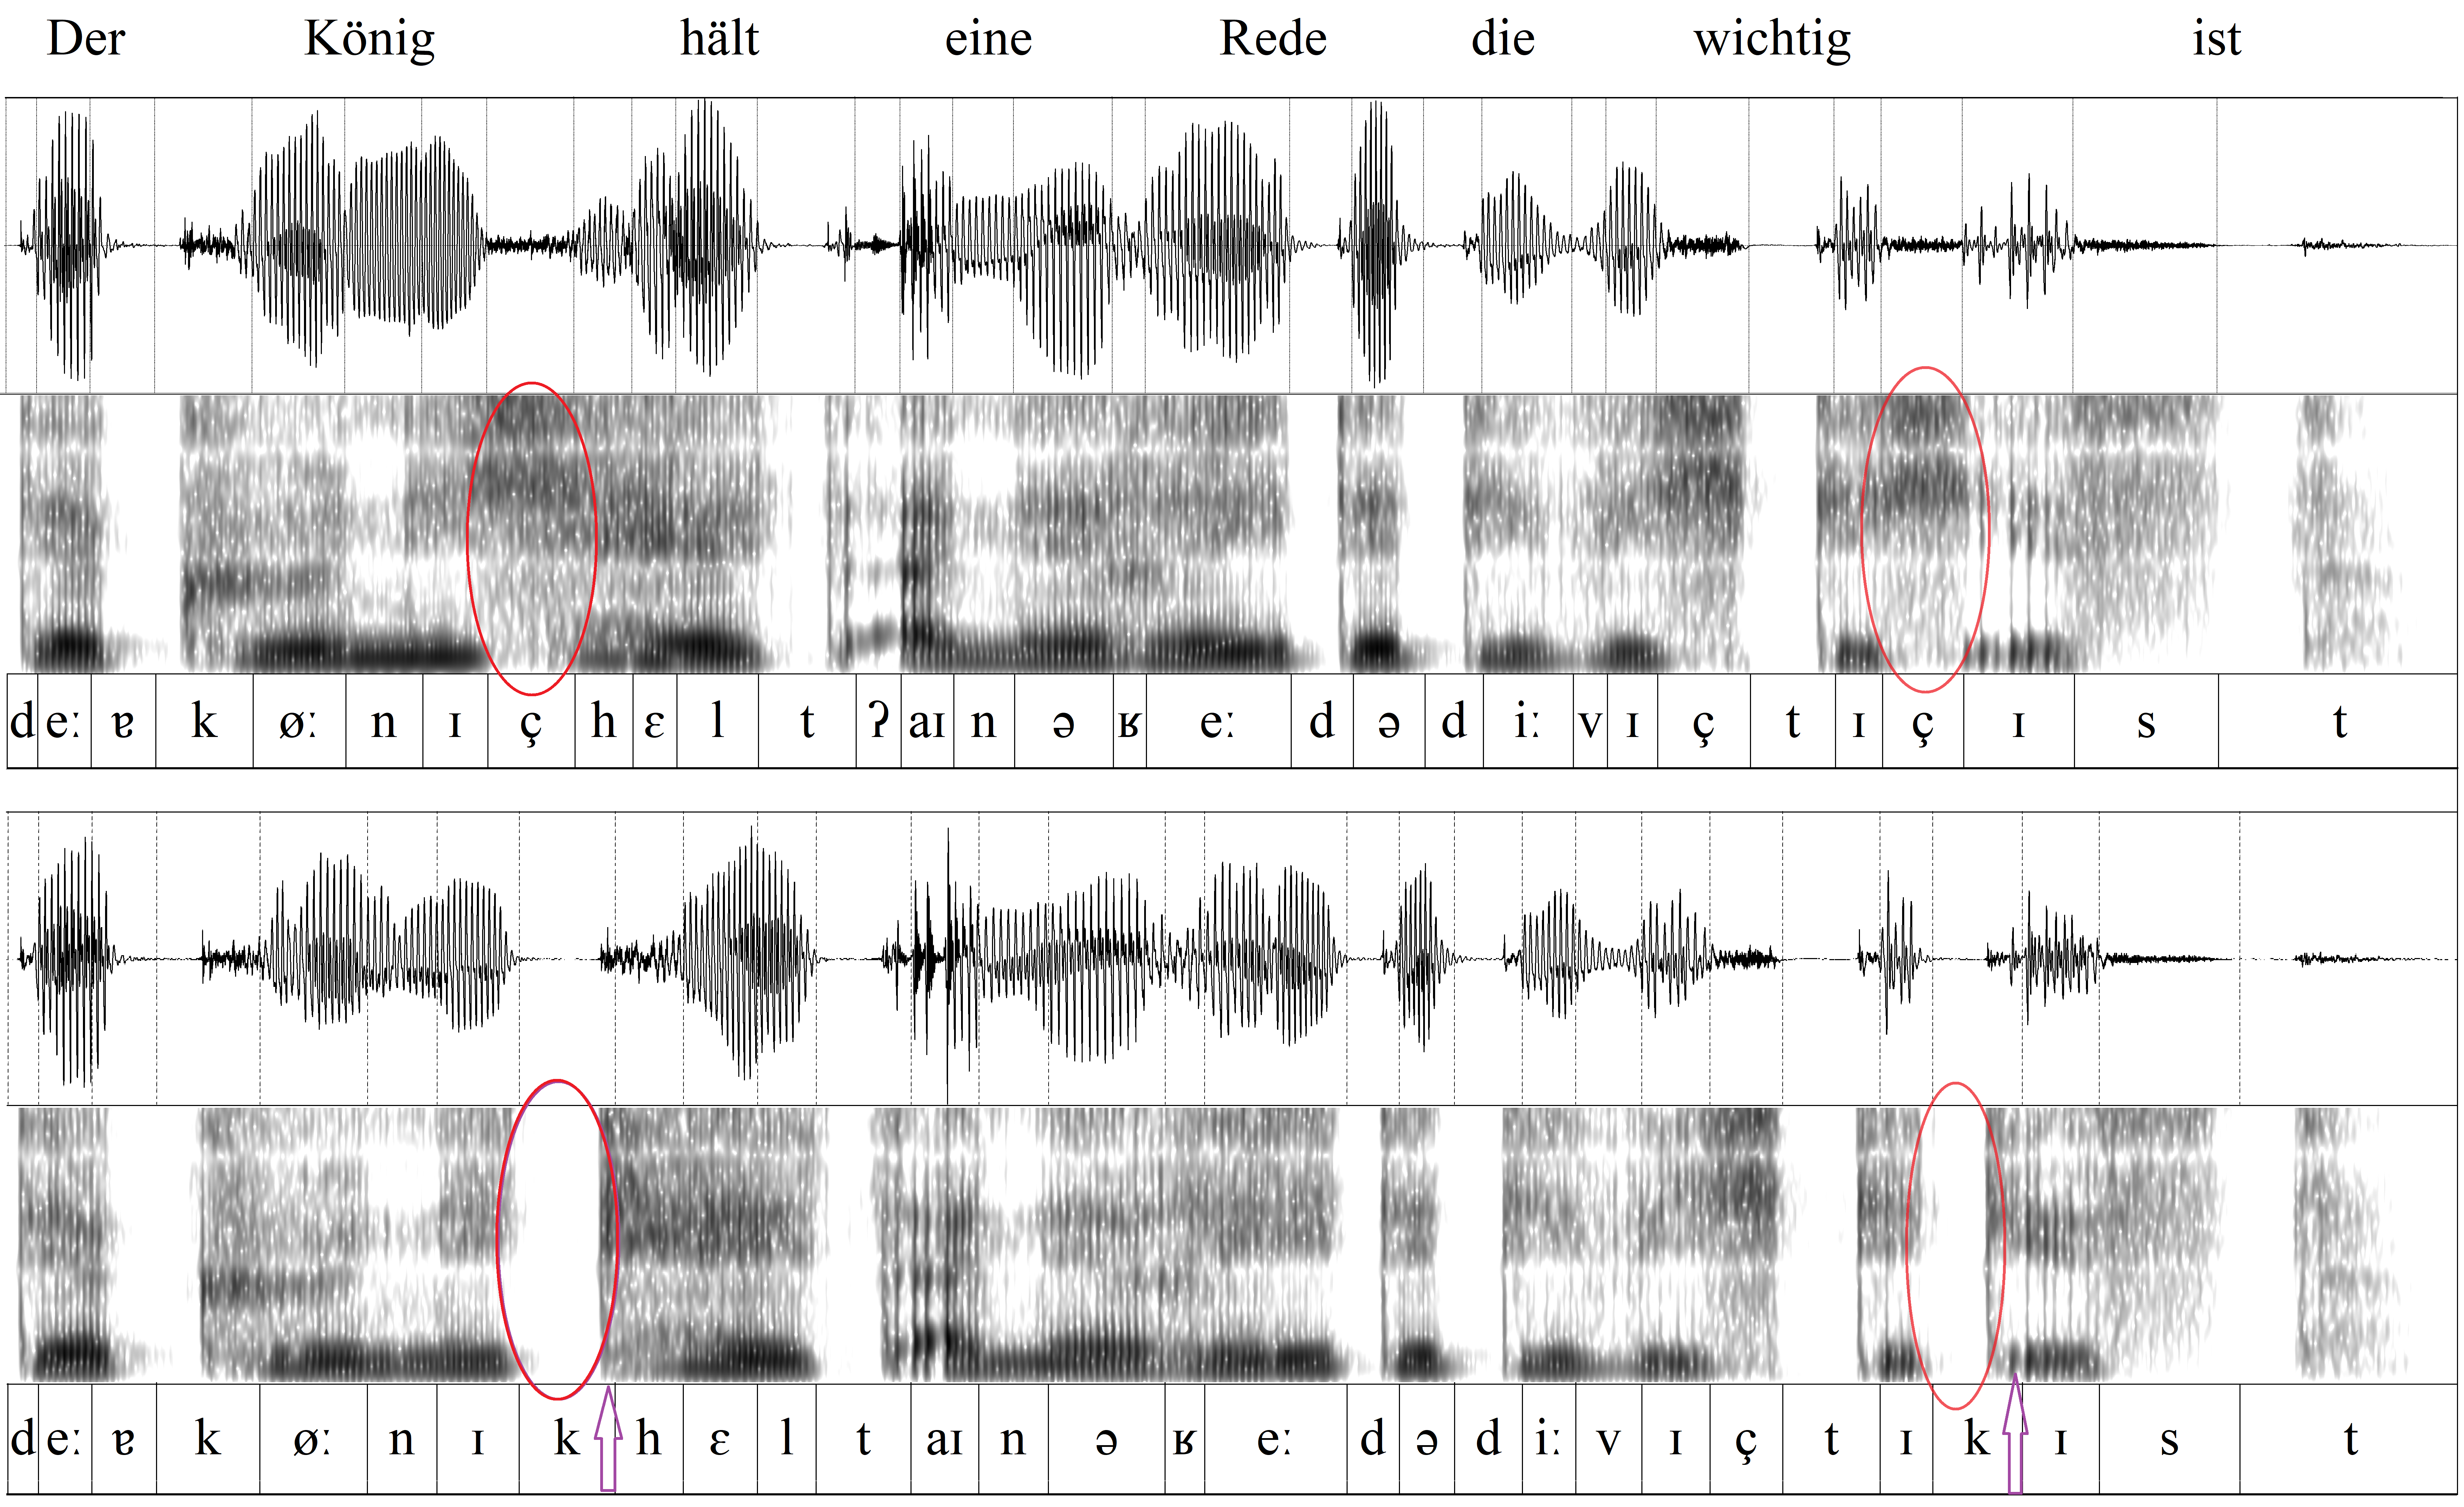
\includegraphics[width=1.5\textwidth]{ic_ik_manipulation}
		\caption[Oscillograms and spectrograms of categorical manipulation comparison]
			{Oscillograms and spectrograms of the word \emph{\enquote{König}} (king) and \emph{\enquote{wichtig}} (important) pronounced originally with \textipa{[\c{c}]} sounds, which were changed into \textipa{[k]} sounds.
			The x-axis shows the chronological phonetic transcription over time (\SI{2.3375}{\second} in total) and the spectrograms' y-axes show the frequencies up to \SI{5000}{\hertz}.
			The segments of the modified phonemes are marked with red circles.
			The purple arrows at the end of the \textipa{[k]} segments show that the model even captured the voicing assimilation a vowel.}
		\label{fig:spectrogram_ic_ik}
	\end{figure}
\end{landscape}
\chapter{Web-Based Responsive Spoken Dialogue System}
\label{chap:web-based_responsive_spoken_dialogue_system}

\lettrine{W}{ith} the ability to simulate accommodation, a complete accommodative \acl{sds} is introduced in this chapter.
Its architecture and various customization possibilities are explained.
The vocal changes are illustrated using dynamic visualizations in the system's \acl{gui}.
A replication of the \acl{hci} experiment is showcased to exhibit the system's capabilities and demonstrate its advantages.

\pagebreak

\acresetall

\section[Overview]{Overview and key aspects}
\label{sec:overview_and_key_aspects}

Simulating and triggering accommodation effects occurring in \ac{hhi} in \acp{sds} takes them one step further toward human-like communication.
The system presented in this chapter encapsulates the knowledge acquired from the experiments in \cref{part:experiments}, the behavior designs developed in \cref{part:modeling}, and the module introduced in \cref{chap:convergence_module_for_sdss}.
It contains mechanisms to track the states and changes of segment and suprasegmental phonetic features during a dialogue.
All analyses are automated and run in real-time, which not only saves a lot of time and manual work typically needed in accommodation studies, but also makes the system more suitable for use in other applications.
A user of the system may be a participant in an experiment, an experimenter designing an experiment or monitoring an ongoing experiment, or a researcher that uses it to analyze existing data.
The system was designed with the following key principles in mind:
%
\begin{description}
	\item[Focus on adaptation] --
	the main goal of the system is to offer a tool for investigating vocal accommodation in \ac{hci} for both online experiments and offline analyses.
	Putting vocal accommodation under the spotlight is the core novel contribution of the system, since very few systems offer such capabilities at all, and with control over the accommodative behavior in particular.
	
	\item[Customizability] --
	the system includes several components that can be modified, either for changing the accommodation behavior itself (features, parameters, etc.) or for changing the settings (e.g., for different experiments).
	This allows experimentation with customized scenarios and configurations that can be easily compared in a controlled, reproducible environment.
	
	\item[Online scalability] --
	the system can run in a web browser without any installations or additional files\footnote{Some features need to be enabled in the browser, like JavaScript and microphone access.
	However, any modern browser should not have any problem supporting all the necessary requirements.
	To increase performance, all speech analyses and processing are done on the server side.}.
	Since the system itself runs on a server, it is also possible to operate multiple instances, each with its own configurations and parameters.
	This makes it easy to distribute its use, e.g., for remotely conducting an experiment where a specific configurations can be given to each participant.
\end{description}
%
This customizable system is a tool that could help to deepen the experimental possibilities and to automate the processes typically involved in accommodation-related experiments.
The system's architecture, \ac{gui}, and functionality are described in \cref{sec:architecture,sec:online_and_offline_modes}.
The experiment presented in \cref{chap:shadowing_in_sung_music_and_human_computer_interaction} is replicated in \cref{sec:showcase} to demonstrate the system's utilization.

\section{Architecture}
\label{sec:architecture}

As the system aims to offer a customizable playground for studying phonetic adaptation in \ac{hci}, a key property of its architecture is the separation between client-side, server-side, and external resources (see \cref{fig:web-based_architecture}).
This separation makes it possible to run multiple clients on different machines at the same time with a single server collecting the data from all of them at the same time.
The server, ideally running on a dedicated machine, is operated by a person responsible for designing and configuring the interactions, e.g., an experimenter.
It collects information and audio recordings from all interactions with the system (which can be deleted afterwards for privacy purposes).
This separation of the server grants the experimenter a lot of freedom and flexibility, since resources like feature configurations and dialogue domain can be modified independently, even while users are using the system.
Additionally, multiple configurations can be prepared in advance (e.g., for different participant groups), regardless of the device the experiment will be performed on and without summoning the participants to the lab.
Configurations can even be changed over the course of the experiment if additional variations are required.
These configurations are transparent to the users, and no action is required from them aside from starting a new interaction with he system.
This flexibility makes it easier and quicker to create new scenarios of interaction and to experiment with different features and parameters.

In addition to the technical advantages, letting users to interact with the system on a separate machine broadens the usage possibilities.
For example, an experiment can be carried out remotely, without the need to invite participants to the recording studio one by one.
Furthermore, as the connection to the server is done via a web browser, participants can connect use the system with their own computers wherever and whenever it suits them, without any additional installation or technical configurations.
All of these make it possible to collect data from many users rapidly and easily.
%
\begin{figure}[t]
	\centering
	\includegraphics[width=\linewidth]{web-based_architecture_no-ajax}
	\caption[Architecture of the web-based system]
		{The architecture of the system.
		The background colors distinguish between client components, server components, and customizable external resources.
		The dashed line coming out of the convergence model's box indicates that the feature predictions may or may not be passed from the model to the system depending on the feature definition and update parameter (see \cref{sec:parameters}).}
	\label{fig:web-based_architecture}
\end{figure}
%
The main components of the system are the \ac{sds} with the accommodation module (\cref{subsec:dialogue_system}), the \ac{gui} (\cref{subsec:graphical_user_interface}), and the external resources and configuration (\cref{subsec:models_and_cusomizations}).

\subsection{Dialogue system}
\label{subsec:dialogue_system}

The core of the system is the dialogue system component (see green block in \cref{fig:web-based_architecture}), which controls the flow of the interaction, processes users' inputs, and generates the system's responses.
It uses the extended architecture presented in \cref{subsec:extended_sds}, which consists of traditional \ac{sds} components such as \ac{nlu} and a \ac{dm}, but also contains the \ac{asp} module that adds accommodation support \citep{Raveh2017SemDial}.
The implementation of this module in the system is as described in \cref{fig:adaptation_module_architecture}.
While the \ac{nlu} component uses merely the transcription provided by the \ac{asr}, the \ac{asp} module analyzes the speech signal itself.
Concretely, it tracks occurrences of the defined features and passes their measured values to the convergence model, as explained in \cref{subsubsec:tracked_features}, which, in turn, forwards the tracked feature parameters to the \ac{tts} synthesis component.
The \ac{tts} engine then takes the text generated by the \ac{nlg} component, and, if phonetic-level manipulation is supported by the \ac{tts} module, synthesizes the utterance using the values specified by the convergence model.
The connection between the dialogue system's modules is managed by the OpenDial framework \citep{Lison2016opendial, Lison2015developing}.
%The \ac{asr} module uses CMUSphinx \citep{Lamere2003sphinx} with additional customized functionality for obtaining the phonetic information required for the \ac{asp} module, and the \ac{tts} is driven by MaryTTS \citep{LeMaguer2017uprooted, Schroeder2003mary}.
The \ac{nlu} and \ac{nlg} modules are built using an OpenDial's domain file, as described in \cref{subsubsec:dialogue_domain}.
Importantly, each of these components can be replaced with another implementation, all time it takes the same input and provides the same type of output.

\subsection{Visualization and \acl{gui}}
\label{subsec:graphical_user_interface}

\afterpage{%
	\begin{landscape}
		\begin{figure}[t]
			\centering
			\vspace*{-4cm}
			\hspace*{-4.7cm}
			\includegraphics[width=1.65\textwidth]{gui}
			\caption[Web system in-browser \acs{gui}]
				{A screenshot of the system's \acl{gui}, with the chat area on the top left, the interaction area on the bottom left, the plot area on the top right, and the notification area on the bottom right.
				In both the chat area and the plot area, the user and system are represented by the colors blue and orange, respectively.}
			\label{fig:gui}
		\end{figure}
	\end{landscape}
}
%
The interaction with the system is done via an in-browser \ac{gui} (see screenshot example in \cref{fig:gui}).
At the top of the screen is a control bar, which offers the user an overview of the interaction and easy access to some general functionalities.
On the left-hand side of the bar, the user can view the list of the interaction's turn history and jump to a specific one.
It is also possible to see the list of tracked features and their current state.
Both lists can be reset using the Reset button (in red), which starts a new interaction using the current configurations (which may have been changed during the ongoing interaction).
On the other side of the bar, there are buttons for viewing on-screen how-to-use information window and changing various settings of the system, like convergence parameters, view options, resource location, etc.
The rest of the \ac{gui} is divided into four areas:
A \emph{chat area} displaying the dialogue turns,
an \emph{interaction area} in which the user provides input to the systems,
a \emph{plot area} with interactive dynamic visualization of the tracked features, and a \emph{notification area} where out-of-conversation messages for the user can be prompted.
The functionality of these areas is described in \crefrange{subsubsec:chat_area}{subsubsec:notification_area}

\subsubsection{Chat area}
\label{subsubsec:chat_area}

The interaction between the user and the system is shown in a chat-like format at the upper left part of the screen.
Each turn's utterance appears inside a bubble with the user's and system's turns represented by different colors.
A bubble always contains a single utterance, regardless of whether a floor change has taken place.
A turn can be replayed at any time using the Play button next to the turn number, corresponding to the turn order on the list accessible from the control bar.
Besides utterance bubbles, the system can also display general-purpose messages related to the interaction, which do not progress the dialogue flow and do count as system utterances.
These messages can be used, for example, to give a participant additional information or further instructions during an experiment.

\subsubsection{Interaction area}
\label{subsubsec:interaction_area}

The user can interact with the system with both written and spoken input using the controls at the bottom left of the screen.
Spoken input can be provided either by speaking \enquote{live} into the microphone or via audio files with pre-recorded speech.
These are typically useful for online and offline usage, respectively (as explained in \cref{sec:online_and_offline_modes}), but pre-recorded utterances can also be useful for reproducing previous experiments or comparing different accommodation configurations with the exact same user input, as done in \cref{app:system_examples}.
Text-based interactions progress through the dialogue (if applicable) and trigger any subsequent module, but will not affect the tracked features, as no vocal input is provided.
This can be useful for quickly going through specific parts of an experiment (like instructions or setup) or for continuing the dialogue without changing the system's representation of the tracked features.

\subsubsection{Plot area}
\label{subsubsec:plot_area}

\begin{figure}[t]
	\centering
	\includegraphics[width=\linewidth]{plot_area}
	\caption[Real-time dynamic visualization of phonetic changes]
		{The plot area showing the states of the feature \textipa{[E:]}~vs.~\textipa{[e:]} during an interaction.
		The system's (orange, bottom right) gradually adapts to the user's (blue, upper left) detected realizations.
		A prediction of the feature's current realization is given for both interlocutors.
		The text box shows the mouse-over annotation of the turn in which the system's realization changed its vowel category.}
	\label{fig:plot}
\end{figure}
%
Visualizations of the tracked features' changes over the course of the interaction are displayed in the upper right part of the screen.
Each feature is visualized separately, and new datapoints are dynamically added whenever applicable.
\Cref{fig:plot} shows an example of such a plot with several accumulated datapoints.
The type of a feature's plot can be defined based on its characteristics, e.g., bars for one-dimensional features and lined scatter plots for two-dimensional features.
These plots are generated using the Plotly library\footnote{\url{https://plot.ly}}, which provides some interactive functionalities.
Hovering over a datapoint in the plot reveals additional information, such as the turn in which it was added, or the realized variant of the feature produced in that turn, as predicted by its classifier (see \cref{subsec:classifiers_training}).

\subsubsection{Notification area}
\label{subsubsec:notification_area}

Whenever a message outside the content of the interaction needs to reach the user, it can be shown at the bottom right part of the screen.
Such messages may include indications of the system's activity, e.g., successful initialization of the interaction, warnings and errors while uploading files, etc.
The notifications can be colored blue, green, orange, or red to indicate the type of the message.

%\subsubsection{Settings and help}
%\label{subsubsec:settings_and_help}
%
%An additional modal window can be called, in which various settings can be changed, and some usage information is provided.
%Configurable settings include the convergence model parameters, domain file, \ac{gui} tweaks, and more.
%These settings can be modified at any point during the interaction, so that it is possible to experiment with different configurations in real-time.
%For persistent changes, it is also possible to edit the configuration file itself, which is loaded when the system starts.
%The usage tab explains the various functionalities of the system and how each area of the \ac{gui} works.
%It also lists special commands that can be executed from text field (used for simulating the user's input, as mentioned in \cref{subsubsec:interaction_area}).
%These commands include printing a short or detailed summary of the phonetic changes throughout the interaction, extracting the data from the features' plots (e.g., for further analysis), and more.
%\todo{screenshot with the settings tab}

\subsection{Customizations}
\label{subsec:models_and_cusomizations}

The system aims to offer a platform for \acp{sds} with convergence support that can be modified and customized according to the user's needs.
All of the aforementioned system components can be customized, at least to some extent.
This includes, among others, the phonetic convergence model, the features tracked by the system, and the dialogue domain.

\subsubsection{Tracked features}
\label{subsubsec:tracked_features}

The accommodation process is initiated by the phonetic features defined in the textual configuration file.
The process is triggered whenever a phoneme associated with a segmental phonetic feature is detected in a segment by the \ac{asr} or for a suprasegmental feature that potentially occurs for in segment.
The feature definitions may capture, for example, general tendencies or specific phonological rules, like schwa elision in German (see \cref{eq:schwa_elision_rule}).
As explained in \cref{subsec:computational_model}, each feature is detected and filtered based on its definition.
This definition can be easily changed to experiment with different accommodation effects.
An example for a feature definition is presented in \cref{subsec:setup_adjustments}.

\subsubsection{Dialogue domain}
\label{subsubsec:dialogue_domain}

The dialogue's flow is specified using OpenDial's XML-based format\footnote{\url{http://www.opendial-toolkit.net/user-manual/dialogue-domains}}.
This format offers a structure for building models, rules, and conditions, which define the \ac{dm} logic.
The rules connect between intents provided by the \ac{nlu} component to the output generated by the \ac{nlg} component.
Additional parameters are used to trigger processing for other modules of the \ac{sds}, like the \ac{asp} module in the system discussed here.
More details about building a domain file can be found in \citet{Lison2016opendial}.
The format of the domain file makes it easy to define new scenarios for the system, like different experimental settings.
Rules are written mostly using regular expressions, which makes it relatively easy also for non-technical users to modify the system's logic.
Since the \ac{dm} keeps track of parameters from all modules, the system's output can even be influenced by the state of the accommodation state in the \ac{asp} module.

\subsubsection{Speech processing}
\label{subsubsec:speech_processing}

Multiple components of the system deal with different aspects of speech processing.
As each module in the system can be replaced independently, different engines and models can be used.
For example, the \ac{asr} engine can be replaced for improving performance or adding support for additional languages.
The \ac{tts} component can be replaced as well, e.g., for changing the voice of the system or offering better control over phonetic manipulations.
The tool used for the phonetic analysis can be changed as well to improve accuracy or performance.
The models and tools described here are those that were used for the showcase presented in \cref{sec:showcase}.
The \ac{asr} component uses CMUSphinx\footnote{Sphinx4 version 5prealpha, \url{https://cmusphinx.github.io/}} \citep{Lamere2003sphinx}, with an extension to the phoneme emission functionality to provide the \ac{asp} module the phonetic input information it needs (see \cref{subsec:computational_model}).
The acoustic model and pronunciation dictionary were taken from CMUSphinx models\footnote{\url{https://sourceforge.net/projects/cmusphinx/files/Acoustic\%20and\%20Language\%20Models/German/}}.
A new language model was created especially for this purposes using SRILM \citep{Stolcke2002SRILM}.
All the segmental and suprasegmental analyses required for the measuring accommodation were done using Praat \citep{Boersma2018praat}.
MaryTTS \citep{LeMaguer2017uprooted, Schroeder2003mary} was used as the \ac{tts} engine of the system, with \texttt{bits1-hsmm} and \texttt{bits3-hsmm} for its female and male voices, respectively.

\section{Online and offline modes}
\label{sec:online_and_offline_modes}

\begin{figure}[t]
	\centering
	\includegraphics[width=0.85\linewidth]{online_offline_small}
	\caption[Online and offline modes of the responsive \acl{sds}]
		{Online (orange) and offline (blue) modes of the system.}
	\label{fig:online_offline_modes}
\end{figure}

The system can operate in two modes, as shown in \cref{fig:online_offline_modes}:
Online -- turn-based real-time interaction via the \ac{gui} (\cref{subsec:graphical_user_interface}); and offline -- on-demand analysis of existing interaction data, either from a recorded online session or a pre-recorded dataset.
The accommodation-related parts of the system (roughly corresponding to the \emph{server} and \emph{resources} blocks in \cref{fig:web-based_architecture}) are common to the two modes, which makes it easy to switch between the two.
The differences are in how the data is fed to the system and how the output is processed and visualized.
The main difference is that in the online mode the process is recurrent and both the user's input and the system's current state are acquired on the fly.
Depending on the scenario defined in the domain file, in online mode there could always be another turn, either of the user or the system, that will continue the interaction.
In the offline mode, the data scope is, by definition, finite.
Technically, the dataset is represented and processed the same way as online interactions, but there is no need to output the system's state to a user.
The common representation also makes it easy to compare pre-recorded interactions with live ones.
However, the output of the accommodation model after each turn is handled differently in both modes.
In online interactions, the output is sent on a turn-by-turn basis to both the web-based \ac{gui} for visualization (as in \cref{fig:plot}) and back to the user as auditory response from the system.
The offline mode doesn't need to interact with a user, so the entire analysis is saved together, along with some additional analyses that can only be preformed with complete interactions.
This output can then be used for further statistical analysis and be visualized separately using other tools (like those in \cref{fig:hds_dds_time,fig:synchrony_switchboard}).
For using the online mode, the system needs to run as a server and be accessed via a web browser.
The offline mode can be used either directly from the command line or programmatically from another application.
A mid-way usage is to manually load pre-recorded files via the \ac{gui} to simulate a live interaction, as explained in \cref{subsubsec:interaction_area}.
While this requires more time and manual effort, it lets the user observe the visualized gradual phonetic changes.

\section{Showcase: replicating a shadowing experiment}
\label{sec:showcase}

As a showcase of the system capabilities, it was utilized to replicate the shadowing experiment described in \cref{sec:convergence_to_natural_and_synthetic_stimuli}.
The experiment is designed to trigger phonetic convergence by confronting the participants with stimuli in which certain phonetic features are realized in a way different from their natural production.
This was done using the offline mode of the system, to simulate a real experiment and automate certain parts of it that would otherwise be performed manually.
The replication used the original stimuli and utterances of the participants.
However, analyses originally done post facto and to different extents manually, like detecting the realized variant, measuring the features' values, etc., are now done automatically.
This demonstrates an automated, reproducible execution, and also offers additional insights via classification of feature realizations and dynamic real-time visualizations.
Finally, using the system the experiment becomes more of a fluent dialogue rather than a experimental simulated interaction, which enhances its \ac{hci} nature.

\subsection{Setup}
\label{subsec:setup_adjustments}

For the experiment replication, two of the three segmental features investigated in the original experiment were used.
In addition to the \textipa{@}-length feature shown in \cref{subsec:computational_model} the feature \textipa{[E:]}~vs.~\textipa{[e:]} was included.
Both features are described in detail in \cref{subsubsec:target_features_HCIConv}, and \cref{tab:target_features} shows example stimulus sentences containing them.
As in the original experiment, the word containing the target features were embedded into 15 short carrier sentences and 25 filler sentences, in which none of the features occur (see \cref{app:shadow_experiment_stimul} for the full stimulus list).
Although both features' underlying values are gradual, they are perceived as two-way categorical variations.
To map these underlying values to a specific variant, a classifier was associated with each feature, as explained in \cref{subsec:classifiers_training}.
The definition of the \textipa{[E:]}~vs.~\textipa{[e:]} features was as follows:
%
%\begin{description}[labelindent=1.5cm, labelwidth=\widthof{\quad \bfseries calculation}]
%	\item[name]	ee\_E
%	\item[phoneme] EHH
%	\item[context] .* EHH .*
%	\item[initial] 451, 2116, 2763
%	\item[minimum] 300, 1500, 2500
%	\item[maximum] 750, 2900, 4800
%	\item[measure] formants
%	\item[calculation] decaying average
%	\item[sensitivity] 0.3
%\end{description}
%
\begin{Verbatim}[tabsize=4, commandchars=\\\{\}]
	- \textbf{`e\_E\_vowel'}:
			\textbf{phoneme}: EHH
			\textbf{context}: '.* EHH .*'
			\textbf{initial}: 450 2100
			\textbf{minimum}: 300 1500
			\textbf{maximum}: 750 2900
			\textbf{measure}: formants
			\textbf{calculation}: decaying average
			\textbf{sensitivity}: 0.3
\end{Verbatim}
%
%The value of the key \emph{measure} is \enquote{formants}, which means that this feature is evaluated by the segment's formant values (as specified in the corresponding signal processing script).
%The values of the \emph{minimum} and \emph{maximum} keys stand for the acceptable value range for this feature.
%This avoids distorted values due to \ac{asr} error and lets the user put their phonetic expertise to use.
\noindent
The values of the keys \texttt{minimum}, \texttt{maximum}, and \texttt{initial} stand for the first two formant frequencies.
The \texttt{calculation} method for this feature is \emph{decaying average} (\cref{eq:decaying_average}), which is similar to the regular average but with each value contributing exponentially less to the final value, so that the last (newest) exemplar contributes the most.
Adding such property to the measure gives more weight to new exemplars that were received chronologically closer to the current turn and thus makes the change more strongly influenced by the productions closer to the accommodation change.
Using this measure comes to support the analogy of the exemplar pool to short-term memory, which remembers recent events better than older ones.

Even though further aspects of the experiment could be automated, the experimental procedure stayed as faithful as possible to the procedure of the original experiment.
The domain file created for the showcase was designed to substitute the role of the experimenter in the shadowing phase (cf.\ \cref{fig:HCIConvFlow}), i.e., mainly presenting and playing the stimuli to the participant.
The stimulus order from the original experiment's baseline phase was preserved and semi-randomized in the shadowing phase using the same logic as in the original.
It was also configured to perform the transitions between the phases.
Although it should be assumed that the user indeed repeats the presented utterance, the system nonetheless verifies that the user's utterance matches the current stimulus using the customized language model described in \cref{subsubsec:speech_processing} before presenting the next stimulus.

% A shortened example of the shadowing phase's flow is shown in \cref{app:dialogue_example}.

%\begin{description}[labelindent=1.3cm, labelwidth=\widthof{\quad \textipa{[I\c{c}]}~vs.~\textipa{[Ik]}}]
%	\item [\textipa{[E:]}~vs.~\textipa{[e:]}] in word-medial $\langle$ä$\rangle$
%	\item [\textipa{[I\c{c}]}~vs.~\textipa{[Ik]}] in word-final $\langle$-ig$\rangle$
%	\item [\textipa{[\s{n}]}~vs.~\textipa{[@n]}] in word-final $\langle$-en$\rangle$
%\end{description}
%\noindent
%
\begin{table}[t]
	\centering
	\begin{tabularx}{\linewidth}{@{}*{5}{l}}
		\toprule
		
		War          	& das          			& Ger\textbf{\underline{ä}}t	& sehr          	& teuer? \\
		\emph{Was} 		& \emph{the} 			& \emph{device}           		& \emph{very} 		& \emph{expensive?} \\[0.3cm]
		
%		Ich          	& bin         			& sücht\textbf{\underline{ig}}	& nach				& Schokolade. \\
%		\emph{I}   		& \emph{am} 			& \emph{addicted}				& \emph{to} 		& \emph{chocolate.} \\[0.1cm]
		
		Wir         	& besuch\textbf{\underline{en}} 						& euch				& bald          & wieder. \\
		\emph{We} 		& \emph{will visit}		& \emph{you} 					& \emph{soon} 		& \emph{again.} \\
		\bottomrule
	\end{tabularx}
	\caption[Example sentence for selected phonetic features]
		{Examples of stimuli containing the target features.
		 Each sentence contains only one feature.
		 A list with all target and filler stimuli can be found in \cref{app:shadow_experiment_stimul} }
	\label{tab:target_features}
\end{table}

\subsection{Classifiers training}
\label{subsec:classifiers_training}

As mentioned above, a classifier can be defined for each tracked feature to let the system determine to which realization category each encountered belongs.
This automates the annotation otherwise done manually by the experimenter during or after the experiment.
In the original shadowing experiment, this includes both the determination of the participants' preferred variation in the baseline phase and the annotation of the participants' realizations in the shadowing phase.
To that end, the associated classifier provides real-time classifications for both the user's and the system's realizations of that feature.
This not only saves time, but also helps to prevent inconsistencies that on-the-fly manual annotation might yield.
With this information available, more meaningful insights can be gained into the variation dynamics over the course of the interaction.
In other applications, like \acp{capt}, this information may be taken into account when deciding on the system's next turn.
The classifiers for the replicated experiment were trained on datasets corresponding to the target features' ranges.
The \textipa{@}-length classifier trained to classify segments shorter and longer than \SI{30}{\milli\second}, and the \textipa{e:/E:} classifier was trained on F1 and F2 values of these vowels produced by female speakers (since for the replication a female participant was chosen as well as a female voice for the system).
While training prior to the interactions is generally sufficient, online fine-tuning is also possible to update a feature's classifier whenever requested by the user, e.g., every time the accommodation model is updated.

Here, a \ac{smo} \citep{Platt1999fast, Platt1998sequential} implementation of the \ac{svm} classifier \citep{Vapnik1998support, Joachims2005support} was used, as the two-way categories of these features are expected to be linearly separable.
Each turn's predictions dynamically added as interactive annotations to the visualization of the relevant features, as illustrated in \cref{fig:plot}.
The training data used for each classifier contains only the productions of the corresponding target feature from a single stimulus set, since these are the productions to which the participants were exposed during the experiment.
This provides relatively few -- but at the same time very precise -- datapoints for each classifier,
which were obtained using the same signal processing technique as the data collected in the experiment.
As explained in \cref{subsubsec:stimuli_participant_hci}, multiple stimulus sets were used in the experiment.
The classification of the system's production was performed based on the stimulus type the participant listened to.
For instance, a classifier trained on the natural stimuli was used when the participant was listening to this stimulus set.

\subsection{Validation}
\label{subsec:validation}

\begin{table}[t]
	\centering
	\begin{tabularx}{\linewidth}{X*{4}{S[table-format=2.1]}}
		\toprule
		sensitivity (\numrange{0}{1}) &  0.2 &  0.3 &  0.4 &  0.5 \\
		adoption (\si{\percent})      & 79   & 86   & 75   & 69   \\
		\bottomrule
	\end{tabularx}
	\caption{The system's convergence degree with different degrees of sensitivity.}
	\label{tab:validation_baseline}
\end{table}

%The validation for the feature \textipa{[E:]}~vs.~\textipa{[e:]} is shown here as a representative example for the phonetic adaptation capability of the system.
For the baseline phase, the degree to which the underlying convergence model accumulated enough data to adopt the user's variant of the feature was examined.
Higher adoption rate indicates a more stable preferred variant of the participant.
The participant's preferred variants was determined based on the majority vote at the end of this phase, as in the original experiment.
For example, if the user realized one variant twice and another three times, the latter was considered the preferred one.
\Cref{tab:validation_baseline} shows the adoption rates of the user's preferred variant as percentages of the mean preferred variant using different values of the \emph{convergence rate} parameter (see \cref{sec:parameters}).
Interestingly, higher values do not necessarily result in higher percentages, due to systematic over-shooting the participant's production in each utterance.
The value 0.3 provided the highest results and was therefore used through the rest of the replication.
See \cref{fig:validation_sensitivity} for visualized examples of the convergence rate's influence.
%
\begin{figure}[t]
	\centering
	\subfigure[The effect of different convergence rates on the change of
			   the system's representation toward the participant's \emph{mean value} for the two-dimensional feature \textipa{[e:]} vs.\ \textipa{[E:]} using decaying average ($\mu = 0.3$).
			   The points represent the calculation steps of the rates 0.1 (red circles), 0.5 (yellow tiranlges), and 0.9 (green rectangles).
			   Each point is the new value calculated after encountering a new exemplar.
			   The common starting point at the top left is the feature's defined initial value.
			   The ellipses represent confidence levels of \SI{90}{\percent}, \SI{50}{\percent}, and \SI{10}{\percent}.]
		{\includegraphics[width=0.47\textwidth]{ee_E_decaying_0.3}
	\label{fig:e_E_bullseye}}
	\hfill
	\subfigure[The effect of different convergence rates for the one-dimensional feature \textipa{@}-length.
			   The bars' height represent the feature's values on the y-axis with the calculation method set to simple average.
			   The x-axis enumerates the feature's updates.
			   The \emph{exemplar} bar shows the feature’s last added exemplar, and the \emph{average} bar
			   is the value of the feature after adding the last exemplar to the pool.
			   Note that the 0-th update appears empty since the initial value of the feature was set to 0.]
		{\includegraphics[width=0.47\textwidth]{schwa_comp_010509}
	\label{fig:schwa_length_bars}}
	\caption[Influence of difference convergence rates on the system's accommodation]
		{Illustration of the effect of different convergence rates on the updates of the system's realization of a two-dimensional feature (left) and a one-dimensional feature (right).}
	\label{fig:validation_sensitivity}
\end{figure}
%
After obtaining the preference of each participant, the degree of convergence was examined per utterance in the shadowing phase.
The participants were grouped based on their convergence behavior in the original experiment:
One group of participants showed low to no tendency to converge (converged in \SI{\le 10}{\percent} of their utterances),
the second had varying degrees of convergence (\SIrange{10}{90}{\percent}),
and the third group of participants who were very sensitive to the stimuli (\SI{\ge 90}{\percent}).
This grouping enables analyses based on collective vocal behaviors instead of individual differences.
The groups were labeled \emph{Low} (\SI{23}{\percent} of participants), \emph{Mid} (\SI{50}{\percent}), and \emph{High} (\SI{27}{\percent}), respectively.
For validation purposes, the shadowing phase was treated as an annotation task of the realized variation in the participants' utterances, where a correct annotation (system produces same variation as the participant) indicates convergence.
The three \enquote{annotators} are the stimuli themselves (\emph{Stim}), the online classification of the system's representation of the feature (\emph{Sys}), and labels from the training dataset used as references (\emph{Ref}).
The Cohen's kappa ($\kappa$) values\footnote{Calculated by the \texttt{kappa2} command of the \texttt{irr} R package, \url{https://cran.r-project.org/package=irr}} are shown in \cref{tab:showcase_results}.
%As expected, the \emph{Low} group has the lowest scores, since these are the participants that converged the least as a whole.
%As \cref{tab:showcase_results} shows, convergence was found in \SI{48}{\percent} of the utterances for \emph{Sys-Stim} and \emph{Ref-Stim} but only in \SI{66}{\percent} for \emph{Ref-Sys}, which means that convergence was found in different instances.
%\todo{not clear what the sentence above wants to say}
\cref{tab:showcase_results} shows that \emph{Ref-Sys} has $\kappa = 0.27$ (fair agreement) for the \emph{Mid} group, but lower scores for the two other groups.
This indicates that the reference values, which supposedly represent some universal average of the feature, indeed match the production of the participants that didn't deviate too greatly from their base production values, which reinforces the fact that the stimuli's influence on them was limited to either direction.
The $\kappa$ values for \emph{Sys-Stim} describe how the system's representations matched the stimuli presented to the participants.
Since the system accommodates to the participants' performance, these values exhibit how similarly the system's productions were to the productions of each participant group.
The \emph{High} group has $\kappa = 0.81$ (strong agreement), indicating a high similarity between these participants and the system, as expected.
Contrarily, the $\kappa$ value for the \emph{Low} group is -0.57 (moderate negative agreement), showing that no convergence -- and potentially even divergence -- occurred with these participants.
% kappa itepratation classes taken from http://www.statisticshowto.com/cohens-kappa-statistic/
These results show that the online predictions made by the system presented here are capable of providing additional insights regarding the accommodation degrees occurring in an interaction.
%
\begin{table}[t]
	\centering
	\caption[Cohen's Kappa scores of system's validation]
		{Percentage of convergence cases and $\kappa$ scores of the three-way convergence comparison for the three participant groups.
		Positive $\kappa$ scores mean agreement between the annotations (here, the feature's realization category) and negative scores indicate disagreement.
		Scores close to zero point to an agreement occurring by chance.}
	\label{tab:showcase_results}
	\begin{tabularx}{\linewidth}{X
								 *{3}{S[table-format=2.0]}
								 @{\hskip 1.4cm}
								 *{3}{S[table-format=1.2, table-space-text-pre={$-$}, table-space-text-post={\,***}]}}
		\toprule
		\multirow{2}{*}{Group} &
		\multicolumn{3}{c}{Convergence cases (\si{\percent})} &
		\multicolumn{3}{c}{Cohen's Kappa ($\kappa$)}\\[0.2cm]
		&
		{\emph{Sys}-\emph{Stim}} & {\emph{Ref}-\emph{Stim}} & {\emph{Ref}-\emph{Sys}} &
		{\emph{Sys}-\emph{Stim}} & {\emph{Ref}-\emph{Stim}} & {\emph{Ref}-\emph{Sys}}\\
		\midrule
		Low		& {<1} &  7 & 16 & -0.57\,*** & -0.08		& 0.17		\\
		Mid		&  22  & 23 & 32 & -0.15\,*   & -0.15\,*	& 0.27\,***	\\
		High	&  26  & 18 & 18 &  0.81\,*** & -0.04		& 0.03		\\[0.2cm]
		All		&  48  & 48 & 66 & -0.11\,*   & -0.13\,**	& 0.21\,***	\\
		\bottomrule
	\end{tabularx}
	\flushleft{\footnotesize \emph{* $p < 0.05$, ** $p < 0.01$, *** $p < 0.001$}}
\end{table}

\chapter*{General discussion}
\label{chap:general_discussion}

\addcontentsline{toc}{chapter}{General discussion}

\acresetall

this is general discussion





\todo[inline]{a part about evaluating accommodation: people are usually not aware of accommodation happening, and if they do, they can't evaluate it in a consistent and reliable way, as it is not necessarily related to measurable features in the acoustic signal}

\citet{Babel2012role} % she says that accommodation evaluation by humans is "holistic" and does not necessarily correlate with specific features in the signal


\citet{Levitan2016implementing} % that's the paper about Levitan's system that entrains in a relatively simple matter. take this as as a baseline when talking about sophistication of system behavior

\todo[inline]{somewhere say that temporal and mutual aspects are emphasized and are usually not in the focus of accommodation research}

%%%%%%%%%%%%%%%%%%%%
% taken from System chapter. use this after talking about what the system can do and maybe some limitations, then this is potential extensions / directions for improvement
Future work will pursue two independent directions:
regarding phonetic convergence, supporting more features will make the system more comprehensive and useful for studying a wider range of phenomena.
Specifically, adding support for supra-segmental (i.e., prosodic) features will enable replication of experiments similar to, e.g., \citet{Levitan2014acoustic, Levitan2016implementing} in the same manner as in \cref{sec:showcase}.

Regarding user acceptance, it would be interesting to examine whether users show any preference toward an \ac{sds} that converges to their speech on the phonetic level, and whether they would change their speaking style based on the system's output, forming an interaction with mutual and dynamic convergence.
The first research question can be tested by comparing user interaction with a baseline system and one with convergence capabilities, and evaluating the users' performance and satisfaction.
The second research question can be investigated by comparing the users' speech when interacting with either system configuration.
Additionally, to test the system's influence on users' speech, the users can train with an intelligent \acf{call} or \acf{capt} system, which will change its learner model based on their input.
Task completion rate, performance accuracy, and completion time metrics can be used to evaluate how helpful the system is.
%%%%%%%%%%%%%%%%%%%%

\todo[inline]{start with saying that accommodation in HCI is still a relatively new research area and there are no common methods for measuring and evaluating this. reasons -- maybe because there is no defined measuring unit, specifically when is comes to changes overtime and not only point vs. point. also, since there is no "correct" and "incorrect" answers, it is hard to compare against some gold standard and say whether results are good.}

\todo[inline]{having common terminology can be a first step toward comparable and common research methods. part of this work is to define some of the terms used to describe the various types of accommodation that could occur and the relations between them (cref).}










\todo[inline]{[1-2 introduction sentences saying that this thesis shows the connection between accommodation in humans, modeling, and technical aspects of accommodation and that they are all important for its understanding]. more often than not, the technical parts of HCI (e.g., ASR accuracy or TTS quality) are designed and developed separately from the user perspective. while this is understandable when the goal is purely the engineering improvements, this is problematic when addressing dialogue-related problems. [1 more connecting sentence]. Since accommodation in HCI involves both computers and humans, both these two sides of the same coin should be considered in the research and development of such systems. [1 more sentence that those need to work together]. In the case of accommodation, investigating effects in humans that are not relevant or cannot be implemented in computers doesn't contribute to the advancement toward accommodative HCI. Similarly, achieving technical goals that are not perceivable by humans or are not based on any human-centric modeling don't provide any added values as well. [give example of MFCC-matching accommodation (can find paper from Specom 2018?)]. [here continue a few more sentences about thinking about accommodation as one large process with several components in it (cref to roadmap figure) and say this encourage closer collaboration of researchers from human, dialogue, and technical areas]}







\todo[inline]{[as a continuation to the technical challenges in modeling accommodation in computers]. not all accommodation capabilities are born equal. this work distinguishes between several \enquote{levels} accommodation capabilities in computers [cref], as demonstrated and discussed in chapters 7 and 8. this concept is not only motivated by the different layers of accommodative behaviors in humans, but also allows for more or less complex design depending in the target application. [2-3 sentences with examples from work and how they can be used and how it is parallel to human behaviors.]}





\todo[inline]{[toward the end, when talking about potential future research directions]. As full, human-like accommodation capabilities still do not exist, it remains to be seen whether and how they will influence end users. First, like in the case of other human-inspired capabilities in computers, not all users might like such capability that makes computer behave more like humans. [a sentence saying that it might be very good but still flawed, leading to the negative effect known as the uncanny valley (reference).] Secondly, as in HHI, some speakers are naturally less sensitive to phonetic changes and might not notice such variations in computers if they produce them. While accommodation effect might still occur, this rises the questions whether this would improve user experience nonetheless and whether developers would want to invest in features that users might not even realize and appreciate. Somewhat ironically, this could only be tested once such systems exist. Finally, even when computers will have achieved advanced accommodation capabilities (vocal and otherwise), they might not be desired by users. Depending on the application and type of agent, people might not \emph{want} their computers to demonstrate such human-like behaviors, especially if they don't necessarily explicitly follow the user's preference. [2-3 more sentence about examples of when this could be indeed useful and desired, e.g., social chatbots or avatars that are designed to closely accompany a person for a long time.]}

% remove header and header line
\fancyhead{}
\renewcommand{\headrulewidth}{0pt}

% Bibliography
% ------------

\newrefcontext[sorting=nyt] % sort entries by (last) name
\printbibliography[heading=bibintoc, title={Bibliography}]

% Appendices
% ----------

\appendix

% re-configure title style for appendices
%\titleformat{\section}{\large\bfseries}{\appendixname~\thesection .}{0.5em}{}
\renewcommand{\thesection}{\Roman{section}}
\renewcommand{\thesubsection}{\thesection.\Roman{subsection}}

\part{Appendices}
\label{part:appendices}

\chapter{Shadowing Experiment Stimuli}
\label{app:shadow_experiment_stimul}

\section*{Recording Fillers}
\begin{enumerate}
	\item Der Schrank wird heute geliefert. (\textit{The cabinet will be delivered today.})
	\item Wo finde ich ein neues Glas. (\textit{Where do I find a new glass?})
	\item Der Markt findet donnerstags statt. (\textit{The market takes place on Thursday.})
	\item Sie wirkt recht gut informiert. (\textit{She seems to be very well informed.})
	\item Ist das der Weg zu dir nach Hause? (\textit{Is this the way to your home?})
\end{enumerate}

\section*{Baseline Fillers}
\begin{enumerate}[resume]
	\item Der Eimer ist aus Plastik. (\textit{The bucket is made of plastik.})
	\item Im Kühlschrank liegt ein Pfirsich. (\textit{There is a peach in the fridge.})
	\item Diese Technik wird noch entwickelt. (\textit{This technique will be further developed.})
	\item Das war sehr höflich von dir. (\textit{That was very nice of you.})
	\item Lena geht heute früher ins Bett. (\textit{Lena goes today early to bed.})
\end{enumerate}

\section*{Experiment Fillers}
\begin{enumerate}[resume]
	\item Die Katze weckt mich immer auf. (\textit{The cat always wakes me up.})
	\item Der Kaffee war ja schon kalt. (\textit{The coffee was already cold.})
	\item Wer fliegt heute in den Urlaub? (\textit{Who flies today on vacation?})
	\item Warum regt er sich denn so auf? (\textit{Why is he so upset?})
	\item Das wird ein schönes Geschenk. (\textit{This will be a pretty present.})
	\item Ich hätte gern zwei kleine Brüder. (\textit{I would gladly have two brothers.})
	\item Das Heft war gestern noch da. (\textit{Yesterday the notebook was still here.})
	\item Die Glühbirne ist leider kaputt. (\textit{Unfortunately the light bulb is  broken.})
	\item Sucht sich Karin eine neue Arbeit? (\textit{Is Karin looking for a new job?})
	\item Wird die Wohnung noch renoviert? (\textit{Will the apartment be renovated?})
	\item Sara hat eine andere Meinung. (\textit{Sara has another opinion.})
	\item Habt ihr das rote Auto erkannt. (\textit{Have you recognized the red car?})
	\item Ich täusche mich so gut wie nie. (\textit{I never delude myself.})
	\item Keiner glaubt diese Geschichte. (\textit{No one believes this story.})
	\item Kommt Fabian auch zu dem Fest. (\textit{Does Fabian come to the festival as well?})
\end{enumerate}

\section*{\textipa{[\c{c}]} vs.\ \textipa{[k]}}
\begin{enumerate}[resume]
	\item Kommt Essig in den Salat? (\textit{Does vinegar come into the salad?})
	\item Der König hält eine Rede. (\textit{The king speaks.})
	\item Kommt Ludwig heute Abend mit? (\textit{Does Ludwig join today evening?})
	\item Es ist ganz schön staubig im Keller. (\textit{It is pretty dusty in the basement.})
	\item Ich bin süchtig nach Schokolade. (\textit{I am addicted to chocolate.})
\end{enumerate}

\section*{\textipa{[e]} vs.\ \textipa{[E]}}
\begin{enumerate}[resume]
	\item Die Bestätigung ist für Tanja. (\textit{The confirmation is for Tanja.})
	\item War das Gerät sehr teuer? (\textit{Was the device very expensive?})
	\item Ich mag die Qualität deiner Tasche. (\textit{I like the quality of your bag.})
	\item Der Schädling sieht aber komisch aus. (\textit{The pest looks funny.})
	\item Wie viel Verspätung hat der Zug? (\textit{How much delay does the train have?})
\end{enumerate}

\section*{\textipa{[@n]} vs.\ \textipa{[\s{n}]}}
\begin{enumerate}[resume]
	\item Sie begleiten dich zur Taufe. (\textit{They are accompanying you to the baptism.})
	\item Wir besuchen euch bald wieder. (\textit{We will visit you soon again.})
	\item Sind die Küchen immer so groß? (\textit{Are the kitchens always so big?})
	\item Wir reden ohne Unterbrechung. (\textit{We are talking without interruption.})
	\item Sind die Affen denn zutraulich? (\textit{Are the monkeys trustful?})
\end{enumerate}

\chapter{System Visualization Examples}
\label{app:system_examples}

The examples presented here are screenshots of the \acl{gui} of the responsive system presented in \cref{chap:web-based_responsive_spoken_dialogue_system}. These examples compare the state of the system's representation of the \textipa{[e]} vs.\ \textipa{[E]} feature after processing the same user input but using different parameter values (see \cref{sec:parameters,tab:comp_model_parameters}).
It can be seen, for example, how higher sensitivity (top right) leads to faster -- but somewhat unstable -- convergence process that generally imitates the user's productions.
In contrast, the convergence at the top left is too slow to be representative of the user's production.
The two bottom examples demonstrate how taking a larger number of previous exemplars into account leads to a more smoothed convergence process toward some global mean (bottom right) as opposed to more rapidly changing productions that follow only the last encountered exemplar (bottom left).

\begin{landscape}
	\begin{figure}[H]
		\centering
		\hspace*{-4.7cm}
		\scalebox{1.5}{%
			\begin{minipage}{.45\linewidth}
				\centering
				\includegraphics[width=\linewidth]{e_E_01_01_10}
			\end{minipage}%
			\hfill
			\begin{minipage}{.45\linewidth}
				\centering
				\includegraphics[width=\linewidth]{e_E_09_09_10}
			\end{minipage}
		}
	\end{figure}
	\begin{figure}[H]
		\centering
		\hspace*{-4.7cm}
		\scalebox{1.5}{%
			\begin{minipage}{.45\linewidth}
				\centering
				\includegraphics[width=\linewidth]{e_E_05_05_1}
			\end{minipage}%
			\hfill
			\begin{minipage}{.45\linewidth}
				\centering
				\includegraphics[width=\linewidth]{e_E_05_05_10}
			\end{minipage}
		}
	\end{figure}
\end{landscape}

\acuseall % mark all acronyms as used (although they were reset at the beginning of each chapter)

% To-Do list
% ----------

\listoftodos[TODO List]

\end{document}